\documentclass[twoside]{book}

% Packages required by doxygen
\usepackage{fixltx2e}
\usepackage{calc}
\usepackage{doxygen}
\usepackage[export]{adjustbox} % also loads graphicx
\usepackage{graphicx}
\usepackage[utf8]{inputenc}
\usepackage{makeidx}
\usepackage{multicol}
\usepackage{multirow}
\PassOptionsToPackage{warn}{textcomp}
\usepackage{textcomp}
\usepackage[nointegrals]{wasysym}
\usepackage[table]{xcolor}

% Font selection
\usepackage[T1]{fontenc}
\usepackage[scaled=.90]{helvet}
\usepackage{courier}
\usepackage{amssymb}
\usepackage{sectsty}
\renewcommand{\familydefault}{\sfdefault}
\allsectionsfont{%
  \fontseries{bc}\selectfont%
  \color{darkgray}%
}
\renewcommand{\DoxyLabelFont}{%
  \fontseries{bc}\selectfont%
  \color{darkgray}%
}
\newcommand{\+}{\discretionary{\mbox{\scriptsize$\hookleftarrow$}}{}{}}

% Page & text layout
\usepackage{geometry}
\geometry{%
  a4paper,%
  top=2.5cm,%
  bottom=2.5cm,%
  left=2.5cm,%
  right=2.5cm%
}
\tolerance=750
\hfuzz=15pt
\hbadness=750
\setlength{\emergencystretch}{15pt}
\setlength{\parindent}{0cm}
\setlength{\parskip}{3ex plus 2ex minus 2ex}
\makeatletter
\renewcommand{\paragraph}{%
  \@startsection{paragraph}{4}{0ex}{-1.0ex}{1.0ex}{%
    \normalfont\normalsize\bfseries\SS@parafont%
  }%
}
\renewcommand{\subparagraph}{%
  \@startsection{subparagraph}{5}{0ex}{-1.0ex}{1.0ex}{%
    \normalfont\normalsize\bfseries\SS@subparafont%
  }%
}
\makeatother

% Headers & footers
\usepackage{fancyhdr}
\pagestyle{fancyplain}
\fancyhead[LE]{\fancyplain{}{\bfseries\thepage}}
\fancyhead[CE]{\fancyplain{}{}}
\fancyhead[RE]{\fancyplain{}{\bfseries\leftmark}}
\fancyhead[LO]{\fancyplain{}{\bfseries\rightmark}}
\fancyhead[CO]{\fancyplain{}{}}
\fancyhead[RO]{\fancyplain{}{\bfseries\thepage}}
\fancyfoot[LE]{\fancyplain{}{}}
\fancyfoot[CE]{\fancyplain{}{}}
\fancyfoot[RE]{\fancyplain{}{\bfseries\scriptsize Generated by Doxygen }}
\fancyfoot[LO]{\fancyplain{}{\bfseries\scriptsize Generated by Doxygen }}
\fancyfoot[CO]{\fancyplain{}{}}
\fancyfoot[RO]{\fancyplain{}{}}
\renewcommand{\footrulewidth}{0.4pt}
\renewcommand{\chaptermark}[1]{%
  \markboth{#1}{}%
}
\renewcommand{\sectionmark}[1]{%
  \markright{\thesection\ #1}%
}

% Indices & bibliography
\usepackage{natbib}
\usepackage[titles]{tocloft}
\setcounter{tocdepth}{3}
\setcounter{secnumdepth}{5}
\makeindex

% Hyperlinks (required, but should be loaded last)
\usepackage{ifpdf}
\ifpdf
  \usepackage[pdftex,pagebackref=true]{hyperref}
\else
  \usepackage[ps2pdf,pagebackref=true]{hyperref}
\fi
\hypersetup{%
  colorlinks=true,%
  linkcolor=blue,%
  citecolor=blue,%
  unicode%
}

% Custom commands
\newcommand{\clearemptydoublepage}{%
  \newpage{\pagestyle{empty}\cleardoublepage}%
}

\usepackage{caption}
\captionsetup{labelsep=space,justification=centering,font={bf},singlelinecheck=off,skip=4pt,position=top}

%===== C O N T E N T S =====

\begin{document}

% Titlepage & ToC
\hypersetup{pageanchor=false,
             bookmarksnumbered=true,
             pdfencoding=unicode
            }
\pagenumbering{alph}
\begin{titlepage}
\vspace*{7cm}
\begin{center}%
{\Large T\+FP Game\+Engine }\\
\vspace*{1cm}
{\large Generated by Doxygen 1.8.14}\\
\end{center}
\end{titlepage}
\clearemptydoublepage
\pagenumbering{roman}
\tableofcontents
\clearemptydoublepage
\pagenumbering{arabic}
\hypersetup{pageanchor=true}

%--- Begin generated contents ---
\chapter{Namespace Index}
\section{Namespace List}
Here is a list of all documented namespaces with brief descriptions\+:\begin{DoxyCompactList}
\item\contentsline{section}{\mbox{\hyperlink{namespacetfp}{tfp}} \\*Ddata i czas Date\+And\+Time }{\pageref{namespacetfp}}{}
\end{DoxyCompactList}

\chapter{Hierarchical Index}
\section{Class Hierarchy}
This inheritance list is sorted roughly, but not completely, alphabetically\+:\begin{DoxyCompactList}
\item \contentsline{section}{tfp\+:\+:Animation}{\pageref{classtfp_1_1_animation}}{}
\item \contentsline{section}{tfp\+:\+:Area\+List\+Class}{\pageref{classtfp_1_1_area_list_class}}{}
\item \contentsline{section}{rapidxml\+:\+:attribute\+\_\+iterator$<$ Ch $>$}{\pageref{classrapidxml_1_1attribute__iterator}}{}
\item \contentsline{section}{tfp\+:\+:Button}{\pageref{classtfp_1_1_button}}{}
\item \contentsline{section}{tfp\+:\+:Camera}{\pageref{classtfp_1_1_camera}}{}
\item \contentsline{section}{tfp\+:\+:Character\+Stats}{\pageref{classtfp_1_1_character_stats}}{}
\begin{DoxyCompactList}
\item \contentsline{section}{tfp\+:\+:Player}{\pageref{classtfp_1_1_player}}{}
\end{DoxyCompactList}
\item \contentsline{section}{tfp\+:\+:Clickable\+Area}{\pageref{classtfp_1_1_clickable_area}}{}
\item \contentsline{section}{tfp\+:\+:Clock\+Class}{\pageref{classtfp_1_1_clock_class}}{}
\item \contentsline{section}{tfp\+:\+:Command\+Block}{\pageref{classtfp_1_1_command_block}}{}
\item \contentsline{section}{tfp\+:\+:Debug\+Class}{\pageref{classtfp_1_1_debug_class}}{}
\item \contentsline{section}{tfp\+:\+:Dragable\+Area}{\pageref{classtfp_1_1_dragable_area}}{}
\item exception\begin{DoxyCompactList}
\item \contentsline{section}{rapidxml\+:\+:parse\+\_\+error}{\pageref{classrapidxml_1_1parse__error}}{}
\end{DoxyCompactList}
\item \contentsline{section}{rapidxml\+:\+:file$<$ Ch $>$}{\pageref{classrapidxml_1_1file}}{}
\item \contentsline{section}{tfp\+:\+:Focus\+Area}{\pageref{classtfp_1_1_focus_area}}{}
\item \contentsline{section}{tfp\+:\+:Font}{\pageref{structtfp_1_1_font}}{}
\item \contentsline{section}{tfp\+:\+:Font\+List\+Class}{\pageref{classtfp_1_1_font_list_class}}{}
\item \contentsline{section}{tfp\+:\+:Game}{\pageref{classtfp_1_1_game}}{}
\item \contentsline{section}{tfp\+:\+:Game\+Manager\+Class}{\pageref{classtfp_1_1_game_manager_class}}{}
\item \contentsline{section}{tfp\+:\+:Generator\+Class}{\pageref{classtfp_1_1_generator_class}}{}
\item \contentsline{section}{tfp\+:\+:Gif}{\pageref{classtfp_1_1_gif}}{}
\item \contentsline{section}{tfp\+:\+:Gif\+List\+Class}{\pageref{classtfp_1_1_gif_list_class}}{}
\item \contentsline{section}{tfp\+:\+:Input\+Area}{\pageref{classtfp_1_1_input_area}}{}
\item \contentsline{section}{tfp\+:\+:Input\+Bar}{\pageref{classtfp_1_1_input_bar}}{}
\item \contentsline{section}{tfp\+:\+:Interface}{\pageref{classtfp_1_1_interface}}{}
\item \contentsline{section}{tfp\+:\+:Item}{\pageref{structtfp_1_1_item}}{}
\item \contentsline{section}{tfp\+:\+:Item\+List\+Class}{\pageref{classtfp_1_1_item_list_class}}{}
\item \contentsline{section}{tfp\+:\+:Item\+Stats}{\pageref{structtfp_1_1_item_stats}}{}
\item \contentsline{section}{tfp\+:\+:Key\+Config\+Class}{\pageref{classtfp_1_1_key_config_class}}{}
\item \contentsline{section}{tfp\+:\+:Language\+Class}{\pageref{classtfp_1_1_language_class}}{}
\item \contentsline{section}{tfp\+:\+:Loading\+Bar}{\pageref{classtfp_1_1_loading_bar}}{}
\item \contentsline{section}{tfp\+:\+:Loading\+Screen\+Class}{\pageref{classtfp_1_1_loading_screen_class}}{}
\item \contentsline{section}{tfp\+:\+:Map}{\pageref{classtfp_1_1_map}}{}
\item \contentsline{section}{rapidxml\+:\+:memory\+\_\+pool$<$ Ch $>$}{\pageref{classrapidxml_1_1memory__pool}}{}
\begin{DoxyCompactList}
\item \contentsline{section}{rapidxml\+:\+:xml\+\_\+document$<$ Ch $>$}{\pageref{classrapidxml_1_1xml__document}}{}
\end{DoxyCompactList}
\item \contentsline{section}{tfp\+:\+:Mouse}{\pageref{classtfp_1_1_mouse}}{}
\item \contentsline{section}{tfp\+:\+:Network\+Client}{\pageref{classtfp_1_1_network_client}}{}
\item \contentsline{section}{tfp\+:\+:Network\+Server}{\pageref{classtfp_1_1_network_server}}{}
\item \contentsline{section}{tfp\+:\+:specialeffects\+:\+:Night}{\pageref{classtfp_1_1specialeffects_1_1_night}}{}
\item \contentsline{section}{tfp\+:\+:Key\+Config\+Class\+:\+:Node}{\pageref{structtfp_1_1_key_config_class_1_1_node}}{}
\item \contentsline{section}{tfp\+:\+:Area\+List\+Class\+:\+:Node}{\pageref{structtfp_1_1_area_list_class_1_1_node}}{}
\item \contentsline{section}{rapidxml\+:\+:node\+\_\+iterator$<$ Ch $>$}{\pageref{classrapidxml_1_1node__iterator}}{}
\item \contentsline{section}{tfp\+:\+:specialeffects\+:\+:Rain}{\pageref{classtfp_1_1specialeffects_1_1_rain}}{}
\item \contentsline{section}{tfp\+:\+:Screen}{\pageref{classtfp_1_1_screen}}{}
\item \contentsline{section}{tfp\+:\+:specialeffects\+:\+:Snow}{\pageref{classtfp_1_1specialeffects_1_1_snow}}{}
\item \contentsline{section}{tfp\+:\+:Sprite\+Creator}{\pageref{classtfp_1_1_sprite_creator}}{}
\item \contentsline{section}{tfp\+:\+:specialeffects\+:\+:Storm}{\pageref{classtfp_1_1specialeffects_1_1_storm}}{}
\item \contentsline{section}{tfp\+:\+:Terrain}{\pageref{structtfp_1_1_terrain}}{}
\item \contentsline{section}{tfp\+:\+:Terrain\+List\+Class}{\pageref{classtfp_1_1_terrain_list_class}}{}
\item \contentsline{section}{tfp\+:\+:Terrain\+Position\+Swap\+Save}{\pageref{structtfp_1_1_terrain_position_swap_save}}{}
\item \contentsline{section}{tfp\+:\+:Text\+Creator}{\pageref{classtfp_1_1_text_creator}}{}
\item \contentsline{section}{tfp\+:\+:Window}{\pageref{classtfp_1_1_window}}{}
\item \contentsline{section}{tfp\+:\+:Window\+Global\+Data\+Class}{\pageref{classtfp_1_1_window_global_data_class}}{}
\item \contentsline{section}{rapidxml\+:\+:xml\+\_\+base$<$ Ch $>$}{\pageref{classrapidxml_1_1xml__base}}{}
\begin{DoxyCompactList}
\item \contentsline{section}{rapidxml\+:\+:xml\+\_\+attribute$<$ Ch $>$}{\pageref{classrapidxml_1_1xml__attribute}}{}
\item \contentsline{section}{rapidxml\+:\+:xml\+\_\+node$<$ Ch $>$}{\pageref{classrapidxml_1_1xml__node}}{}
\begin{DoxyCompactList}
\item \contentsline{section}{rapidxml\+:\+:xml\+\_\+document$<$ Ch $>$}{\pageref{classrapidxml_1_1xml__document}}{}
\end{DoxyCompactList}
\end{DoxyCompactList}
\end{DoxyCompactList}

\chapter{Class Index}
\section{Class List}
Here are the classes, structs, unions and interfaces with brief descriptions\+:\begin{DoxyCompactList}
\item\contentsline{section}{\mbox{\hyperlink{classtfp_1_1_animation}{tfp\+::\+Animation}} }{\pageref{classtfp_1_1_animation}}{}
\item\contentsline{section}{\mbox{\hyperlink{classtfp_1_1_area_list_class}{tfp\+::\+Area\+List\+Class}} }{\pageref{classtfp_1_1_area_list_class}}{}
\item\contentsline{section}{\mbox{\hyperlink{classrapidxml_1_1attribute__iterator}{rapidxml\+::attribute\+\_\+iterator$<$ Ch $>$}} \\*Iterator of child attributes of \mbox{\hyperlink{classrapidxml_1_1xml__node}{xml\+\_\+node}} }{\pageref{classrapidxml_1_1attribute__iterator}}{}
\item\contentsline{section}{\mbox{\hyperlink{classtfp_1_1_button}{tfp\+::\+Button}} }{\pageref{classtfp_1_1_button}}{}
\item\contentsline{section}{\mbox{\hyperlink{classtfp_1_1_camera}{tfp\+::\+Camera}} }{\pageref{classtfp_1_1_camera}}{}
\item\contentsline{section}{\mbox{\hyperlink{classtfp_1_1_character_stats}{tfp\+::\+Character\+Stats}} }{\pageref{classtfp_1_1_character_stats}}{}
\item\contentsline{section}{\mbox{\hyperlink{classtfp_1_1_clickable_area}{tfp\+::\+Clickable\+Area}} }{\pageref{classtfp_1_1_clickable_area}}{}
\item\contentsline{section}{\mbox{\hyperlink{classtfp_1_1_clock_class}{tfp\+::\+Clock\+Class}} }{\pageref{classtfp_1_1_clock_class}}{}
\item\contentsline{section}{\mbox{\hyperlink{classtfp_1_1_command_block}{tfp\+::\+Command\+Block}} }{\pageref{classtfp_1_1_command_block}}{}
\item\contentsline{section}{\mbox{\hyperlink{classtfp_1_1_debug_class}{tfp\+::\+Debug\+Class}} }{\pageref{classtfp_1_1_debug_class}}{}
\item\contentsline{section}{\mbox{\hyperlink{classtfp_1_1_dragable_area}{tfp\+::\+Dragable\+Area}} }{\pageref{classtfp_1_1_dragable_area}}{}
\item\contentsline{section}{\mbox{\hyperlink{classrapidxml_1_1file}{rapidxml\+::file$<$ Ch $>$}} \\*Represents data loaded from a file }{\pageref{classrapidxml_1_1file}}{}
\item\contentsline{section}{\mbox{\hyperlink{classtfp_1_1_focus_area}{tfp\+::\+Focus\+Area}} }{\pageref{classtfp_1_1_focus_area}}{}
\item\contentsline{section}{\mbox{\hyperlink{structtfp_1_1_font}{tfp\+::\+Font}} }{\pageref{structtfp_1_1_font}}{}
\item\contentsline{section}{\mbox{\hyperlink{classtfp_1_1_font_list_class}{tfp\+::\+Font\+List\+Class}} }{\pageref{classtfp_1_1_font_list_class}}{}
\item\contentsline{section}{\mbox{\hyperlink{classtfp_1_1_game}{tfp\+::\+Game}} }{\pageref{classtfp_1_1_game}}{}
\item\contentsline{section}{\mbox{\hyperlink{classtfp_1_1_game_manager_class}{tfp\+::\+Game\+Manager\+Class}} }{\pageref{classtfp_1_1_game_manager_class}}{}
\item\contentsline{section}{\mbox{\hyperlink{classtfp_1_1_generator_class}{tfp\+::\+Generator\+Class}} }{\pageref{classtfp_1_1_generator_class}}{}
\item\contentsline{section}{\mbox{\hyperlink{classtfp_1_1_gif}{tfp\+::\+Gif}} }{\pageref{classtfp_1_1_gif}}{}
\item\contentsline{section}{\mbox{\hyperlink{classtfp_1_1_gif_list_class}{tfp\+::\+Gif\+List\+Class}} }{\pageref{classtfp_1_1_gif_list_class}}{}
\item\contentsline{section}{\mbox{\hyperlink{classtfp_1_1_input_area}{tfp\+::\+Input\+Area}} }{\pageref{classtfp_1_1_input_area}}{}
\item\contentsline{section}{\mbox{\hyperlink{classtfp_1_1_input_bar}{tfp\+::\+Input\+Bar}} }{\pageref{classtfp_1_1_input_bar}}{}
\item\contentsline{section}{\mbox{\hyperlink{classtfp_1_1_interface}{tfp\+::\+Interface}} }{\pageref{classtfp_1_1_interface}}{}
\item\contentsline{section}{\mbox{\hyperlink{structtfp_1_1_item}{tfp\+::\+Item}} }{\pageref{structtfp_1_1_item}}{}
\item\contentsline{section}{\mbox{\hyperlink{classtfp_1_1_item_list_class}{tfp\+::\+Item\+List\+Class}} }{\pageref{classtfp_1_1_item_list_class}}{}
\item\contentsline{section}{\mbox{\hyperlink{structtfp_1_1_item_stats}{tfp\+::\+Item\+Stats}} }{\pageref{structtfp_1_1_item_stats}}{}
\item\contentsline{section}{\mbox{\hyperlink{classtfp_1_1_key_config_class}{tfp\+::\+Key\+Config\+Class}} }{\pageref{classtfp_1_1_key_config_class}}{}
\item\contentsline{section}{\mbox{\hyperlink{classtfp_1_1_language_class}{tfp\+::\+Language\+Class}} }{\pageref{classtfp_1_1_language_class}}{}
\item\contentsline{section}{\mbox{\hyperlink{classtfp_1_1_loading_bar}{tfp\+::\+Loading\+Bar}} }{\pageref{classtfp_1_1_loading_bar}}{}
\item\contentsline{section}{\mbox{\hyperlink{classtfp_1_1_loading_screen_class}{tfp\+::\+Loading\+Screen\+Class}} }{\pageref{classtfp_1_1_loading_screen_class}}{}
\item\contentsline{section}{\mbox{\hyperlink{classtfp_1_1_map}{tfp\+::\+Map}} }{\pageref{classtfp_1_1_map}}{}
\item\contentsline{section}{\mbox{\hyperlink{classrapidxml_1_1memory__pool}{rapidxml\+::memory\+\_\+pool$<$ Ch $>$}} }{\pageref{classrapidxml_1_1memory__pool}}{}
\item\contentsline{section}{\mbox{\hyperlink{classtfp_1_1_mouse}{tfp\+::\+Mouse}} }{\pageref{classtfp_1_1_mouse}}{}
\item\contentsline{section}{\mbox{\hyperlink{classtfp_1_1_network_client}{tfp\+::\+Network\+Client}} }{\pageref{classtfp_1_1_network_client}}{}
\item\contentsline{section}{\mbox{\hyperlink{classtfp_1_1_network_server}{tfp\+::\+Network\+Server}} }{\pageref{classtfp_1_1_network_server}}{}
\item\contentsline{section}{\mbox{\hyperlink{classtfp_1_1specialeffects_1_1_night}{tfp\+::specialeffects\+::\+Night}} }{\pageref{classtfp_1_1specialeffects_1_1_night}}{}
\item\contentsline{section}{\mbox{\hyperlink{structtfp_1_1_key_config_class_1_1_node}{tfp\+::\+Key\+Config\+Class\+::\+Node}} }{\pageref{structtfp_1_1_key_config_class_1_1_node}}{}
\item\contentsline{section}{\mbox{\hyperlink{structtfp_1_1_area_list_class_1_1_node}{tfp\+::\+Area\+List\+Class\+::\+Node}} }{\pageref{structtfp_1_1_area_list_class_1_1_node}}{}
\item\contentsline{section}{\mbox{\hyperlink{classrapidxml_1_1node__iterator}{rapidxml\+::node\+\_\+iterator$<$ Ch $>$}} \\*Iterator of child nodes of \mbox{\hyperlink{classrapidxml_1_1xml__node}{xml\+\_\+node}} }{\pageref{classrapidxml_1_1node__iterator}}{}
\item\contentsline{section}{\mbox{\hyperlink{classrapidxml_1_1parse__error}{rapidxml\+::parse\+\_\+error}} }{\pageref{classrapidxml_1_1parse__error}}{}
\item\contentsline{section}{\mbox{\hyperlink{classtfp_1_1_player}{tfp\+::\+Player}} }{\pageref{classtfp_1_1_player}}{}
\item\contentsline{section}{\mbox{\hyperlink{classtfp_1_1specialeffects_1_1_rain}{tfp\+::specialeffects\+::\+Rain}} }{\pageref{classtfp_1_1specialeffects_1_1_rain}}{}
\item\contentsline{section}{\mbox{\hyperlink{classtfp_1_1_screen}{tfp\+::\+Screen}} }{\pageref{classtfp_1_1_screen}}{}
\item\contentsline{section}{\mbox{\hyperlink{classtfp_1_1specialeffects_1_1_snow}{tfp\+::specialeffects\+::\+Snow}} }{\pageref{classtfp_1_1specialeffects_1_1_snow}}{}
\item\contentsline{section}{\mbox{\hyperlink{classtfp_1_1_sprite_creator}{tfp\+::\+Sprite\+Creator}} }{\pageref{classtfp_1_1_sprite_creator}}{}
\item\contentsline{section}{\mbox{\hyperlink{classtfp_1_1specialeffects_1_1_storm}{tfp\+::specialeffects\+::\+Storm}} }{\pageref{classtfp_1_1specialeffects_1_1_storm}}{}
\item\contentsline{section}{\mbox{\hyperlink{structtfp_1_1_terrain}{tfp\+::\+Terrain}} }{\pageref{structtfp_1_1_terrain}}{}
\item\contentsline{section}{\mbox{\hyperlink{classtfp_1_1_terrain_list_class}{tfp\+::\+Terrain\+List\+Class}} }{\pageref{classtfp_1_1_terrain_list_class}}{}
\item\contentsline{section}{\mbox{\hyperlink{structtfp_1_1_terrain_position_swap_save}{tfp\+::\+Terrain\+Position\+Swap\+Save}} }{\pageref{structtfp_1_1_terrain_position_swap_save}}{}
\item\contentsline{section}{\mbox{\hyperlink{classtfp_1_1_text_creator}{tfp\+::\+Text\+Creator}} }{\pageref{classtfp_1_1_text_creator}}{}
\item\contentsline{section}{\mbox{\hyperlink{classtfp_1_1_window}{tfp\+::\+Window}} }{\pageref{classtfp_1_1_window}}{}
\item\contentsline{section}{\mbox{\hyperlink{classtfp_1_1_window_global_data_class}{tfp\+::\+Window\+Global\+Data\+Class}} }{\pageref{classtfp_1_1_window_global_data_class}}{}
\item\contentsline{section}{\mbox{\hyperlink{classrapidxml_1_1xml__attribute}{rapidxml\+::xml\+\_\+attribute$<$ Ch $>$}} }{\pageref{classrapidxml_1_1xml__attribute}}{}
\item\contentsline{section}{\mbox{\hyperlink{classrapidxml_1_1xml__base}{rapidxml\+::xml\+\_\+base$<$ Ch $>$}} }{\pageref{classrapidxml_1_1xml__base}}{}
\item\contentsline{section}{\mbox{\hyperlink{classrapidxml_1_1xml__document}{rapidxml\+::xml\+\_\+document$<$ Ch $>$}} }{\pageref{classrapidxml_1_1xml__document}}{}
\item\contentsline{section}{\mbox{\hyperlink{classrapidxml_1_1xml__node}{rapidxml\+::xml\+\_\+node$<$ Ch $>$}} }{\pageref{classrapidxml_1_1xml__node}}{}
\end{DoxyCompactList}

\chapter{File Index}
\section{File List}
Here is a list of all documented files with brief descriptions\+:\begin{DoxyCompactList}
\item\contentsline{section}{{\bfseries animation.\+hpp} }{\pageref{animation_8hpp}}{}
\item\contentsline{section}{{\bfseries area.\+hpp} }{\pageref{area_8hpp}}{}
\item\contentsline{section}{{\bfseries button.\+hpp} }{\pageref{button_8hpp}}{}
\item\contentsline{section}{{\bfseries camera.\+hpp} }{\pageref{camera_8hpp}}{}
\item\contentsline{section}{{\bfseries character.\+hpp} }{\pageref{character_8hpp}}{}
\item\contentsline{section}{{\bfseries classpredeclaration.\+hpp} }{\pageref{classpredeclaration_8hpp}}{}
\item\contentsline{section}{{\bfseries client.\+hpp} }{\pageref{client_8hpp}}{}
\item\contentsline{section}{{\bfseries clock.\+hpp} }{\pageref{clock_8hpp}}{}
\item\contentsline{section}{{\bfseries commandblock.\+hpp} }{\pageref{commandblock_8hpp}}{}
\item\contentsline{section}{{\bfseries datatypes.\+hpp} }{\pageref{datatypes_8hpp}}{}
\item\contentsline{section}{{\bfseries dateandtime.\+hpp} }{\pageref{dateandtime_8hpp}}{}
\item\contentsline{section}{{\bfseries debug.\+hpp} }{\pageref{debug_8hpp}}{}
\item\contentsline{section}{{\bfseries defines.\+hpp} }{\pageref{defines_8hpp}}{}
\item\contentsline{section}{{\bfseries filesystem.\+hpp} }{\pageref{filesystem_8hpp}}{}
\item\contentsline{section}{{\bfseries font.\+hpp} }{\pageref{font_8hpp}}{}
\item\contentsline{section}{{\bfseries game.\+hpp} }{\pageref{game_8hpp}}{}
\item\contentsline{section}{{\bfseries gamemanager.\+hpp} }{\pageref{gamemanager_8hpp}}{}
\item\contentsline{section}{{\bfseries generator.\+hpp} }{\pageref{generator_8hpp}}{}
\item\contentsline{section}{{\bfseries globalobjects.\+hpp} }{\pageref{globalobjects_8hpp}}{}
\item\contentsline{section}{{\bfseries includes.\+hpp} }{\pageref{includes_8hpp}}{}
\item\contentsline{section}{{\bfseries interface.\+hpp} }{\pageref{interface_8hpp}}{}
\item\contentsline{section}{{\bfseries interfaceffects.\+hpp} }{\pageref{interfaceffects_8hpp}}{}
\item\contentsline{section}{{\bfseries item.\+hpp} }{\pageref{item_8hpp}}{}
\item\contentsline{section}{{\bfseries keyconfiguration.\+hpp} }{\pageref{keyconfiguration_8hpp}}{}
\item\contentsline{section}{{\bfseries language.\+hpp} }{\pageref{language_8hpp}}{}
\item\contentsline{section}{{\bfseries loading.\+hpp} }{\pageref{loading_8hpp}}{}
\item\contentsline{section}{{\bfseries map.\+hpp} }{\pageref{map_8hpp}}{}
\item\contentsline{section}{{\bfseries mouse.\+hpp} }{\pageref{mouse_8hpp}}{}
\item\contentsline{section}{{\bfseries notes.\+hpp} }{\pageref{notes_8hpp}}{}
\item\contentsline{section}{{\bfseries pixelperfectcollision.\+hpp} }{\pageref{pixelperfectcollision_8hpp}}{}
\item\contentsline{section}{{\bfseries popupwindow.\+hpp} }{\pageref{popupwindow_8hpp}}{}
\item\contentsline{section}{\mbox{\hyperlink{rapidxml_8hpp}{rapidxml.\+hpp}} \\*This file contains rapidxml parser and D\+OM implementation }{\pageref{rapidxml_8hpp}}{}
\item\contentsline{section}{\mbox{\hyperlink{rapidxml__iterators_8hpp}{rapidxml\+\_\+iterators.\+hpp}} \\*This file contains rapidxml iterators }{\pageref{rapidxml__iterators_8hpp}}{}
\item\contentsline{section}{\mbox{\hyperlink{rapidxml__print_8hpp}{rapidxml\+\_\+print.\+hpp}} \\*This file contains rapidxml printer implementation }{\pageref{rapidxml__print_8hpp}}{}
\item\contentsline{section}{\mbox{\hyperlink{rapidxml__utils_8hpp}{rapidxml\+\_\+utils.\+hpp}} }{\pageref{rapidxml__utils_8hpp}}{}
\item\contentsline{section}{{\bfseries screen.\+hpp} }{\pageref{screen_8hpp}}{}
\item\contentsline{section}{{\bfseries server.\+hpp} }{\pageref{server_8hpp}}{}
\item\contentsline{section}{{\bfseries sprite.\+hpp} }{\pageref{sprite_8hpp}}{}
\item\contentsline{section}{{\bfseries terrain.\+hpp} }{\pageref{terrain_8hpp}}{}
\item\contentsline{section}{{\bfseries text.\+hpp} }{\pageref{text_8hpp}}{}
\item\contentsline{section}{{\bfseries textmanipulation.\+hpp} }{\pageref{textmanipulation_8hpp}}{}
\item\contentsline{section}{{\bfseries tfpstl.\+hpp} }{\pageref{tfpstl_8hpp}}{}
\item\contentsline{section}{{\bfseries window.\+hpp} }{\pageref{window_8hpp}}{}
\end{DoxyCompactList}

\chapter{Namespace Documentation}
\hypertarget{namespacetfp}{}\section{tfp Namespace Reference}
\label{namespacetfp}\index{tfp@{tfp}}


Ddata i czas Date\+And\+Time.  


\subsection*{Classes}
\begin{DoxyCompactItemize}
\item 
class \mbox{\hyperlink{classtfp_1_1_animation}{Animation}}
\item 
class \mbox{\hyperlink{classtfp_1_1_area_list_class}{Area\+List\+Class}}
\item 
class \mbox{\hyperlink{classtfp_1_1_button}{Button}}
\item 
class \mbox{\hyperlink{classtfp_1_1_camera}{Camera}}
\item 
class \mbox{\hyperlink{classtfp_1_1_character_stats}{Character\+Stats}}
\item 
class \mbox{\hyperlink{classtfp_1_1_clickable_area}{Clickable\+Area}}
\item 
class \mbox{\hyperlink{classtfp_1_1_clock_class}{Clock\+Class}}
\item 
class \mbox{\hyperlink{classtfp_1_1_command_block}{Command\+Block}}
\item 
class \mbox{\hyperlink{classtfp_1_1_debug_class}{Debug\+Class}}
\item 
class \mbox{\hyperlink{classtfp_1_1_dragable_area}{Dragable\+Area}}
\item 
class \mbox{\hyperlink{classtfp_1_1_focus_area}{Focus\+Area}}
\item 
struct \mbox{\hyperlink{structtfp_1_1_font}{Font}}
\item 
class \mbox{\hyperlink{classtfp_1_1_font_list_class}{Font\+List\+Class}}
\item 
class \mbox{\hyperlink{classtfp_1_1_game}{Game}}
\item 
class \mbox{\hyperlink{classtfp_1_1_game_manager_class}{Game\+Manager\+Class}}
\item 
class \mbox{\hyperlink{classtfp_1_1_generator_class}{Generator\+Class}}
\item 
class \mbox{\hyperlink{classtfp_1_1_gif}{Gif}}
\item 
class \mbox{\hyperlink{classtfp_1_1_gif_list_class}{Gif\+List\+Class}}
\item 
class \mbox{\hyperlink{classtfp_1_1_input_area}{Input\+Area}}
\item 
class \mbox{\hyperlink{classtfp_1_1_input_bar}{Input\+Bar}}
\item 
class \mbox{\hyperlink{classtfp_1_1_interface}{Interface}}
\item 
struct \mbox{\hyperlink{structtfp_1_1_item}{Item}}
\item 
class \mbox{\hyperlink{classtfp_1_1_item_list_class}{Item\+List\+Class}}
\item 
struct \mbox{\hyperlink{structtfp_1_1_item_stats}{Item\+Stats}}
\item 
class \mbox{\hyperlink{classtfp_1_1_key_config_class}{Key\+Config\+Class}}
\item 
class \mbox{\hyperlink{classtfp_1_1_language_class}{Language\+Class}}
\item 
class \mbox{\hyperlink{classtfp_1_1_loading_bar}{Loading\+Bar}}
\item 
class \mbox{\hyperlink{classtfp_1_1_loading_screen_class}{Loading\+Screen\+Class}}
\item 
class \mbox{\hyperlink{classtfp_1_1_map}{Map}}
\item 
class \mbox{\hyperlink{classtfp_1_1_mouse}{Mouse}}
\item 
class \mbox{\hyperlink{classtfp_1_1_network_client}{Network\+Client}}
\item 
class \mbox{\hyperlink{classtfp_1_1_network_server}{Network\+Server}}
\item 
class \mbox{\hyperlink{classtfp_1_1_player}{Player}}
\item 
class \mbox{\hyperlink{classtfp_1_1_screen}{Screen}}
\item 
class \mbox{\hyperlink{classtfp_1_1_sprite_creator}{Sprite\+Creator}}
\item 
struct \mbox{\hyperlink{structtfp_1_1_terrain}{Terrain}}
\item 
class \mbox{\hyperlink{classtfp_1_1_terrain_list_class}{Terrain\+List\+Class}}
\item 
struct \mbox{\hyperlink{structtfp_1_1_terrain_position_swap_save}{Terrain\+Position\+Swap\+Save}}
\item 
class \mbox{\hyperlink{classtfp_1_1_text_creator}{Text\+Creator}}
\item 
class \mbox{\hyperlink{classtfp_1_1_window}{Window}}
\item 
class \mbox{\hyperlink{classtfp_1_1_window_global_data_class}{Window\+Global\+Data\+Class}}
\end{DoxyCompactItemize}
\subsection*{Enumerations}
\begin{DoxyCompactItemize}
\item 
\mbox{\Hypertarget{namespacetfp_a830afe4d34d5aece65b0ca6ab314ff55}\label{namespacetfp_a830afe4d34d5aece65b0ca6ab314ff55}} 
enum {\bfseries Alignment} \{ {\bfseries Align\+Left}, 
{\bfseries Align\+Center}, 
{\bfseries Align\+Right}
 \}
\item 
\mbox{\Hypertarget{namespacetfp_abbe207404383a3069f9ce155ce91f007}\label{namespacetfp_abbe207404383a3069f9ce155ce91f007}} 
enum {\bfseries Direction} \{ {\bfseries Dir\+Top}, 
{\bfseries Dir\+Down}, 
{\bfseries Dir\+Left}, 
{\bfseries Dir\+Right}
 \}
\item 
\mbox{\Hypertarget{namespacetfp_ac199658ccc07707523b27b2607e2682e}\label{namespacetfp_ac199658ccc07707523b27b2607e2682e}} 
enum {\bfseries Text\+Type} \{ {\bfseries Text\+Type\+String}, 
{\bfseries Text\+Type\+Int}, 
{\bfseries Text\+Type\+Float}, 
{\bfseries Text\+Type\+Key}
 \}
\end{DoxyCompactItemize}
\subsection*{Functions}
\begin{DoxyCompactItemize}
\item 
\mbox{\Hypertarget{namespacetfp_a335f3090b47c35efa78618ed7442a989}\label{namespacetfp_a335f3090b47c35efa78618ed7442a989}} 
time\+\_\+t \mbox{\hyperlink{namespacetfp_a335f3090b47c35efa78618ed7442a989}{Seconds}} ()
\begin{DoxyCompactList}\small\item\em Zwraca ilosc sekund od 1970 roku. \end{DoxyCompactList}\item 
std\+::string \mbox{\hyperlink{namespacetfp_aab9c5625cca52707bd8c9c24f331a564}{Date}} (std\+::string Format, time\+\_\+t Time=time(nullptr))
\item 
\mbox{\Hypertarget{namespacetfp_ac66771aedc99f0fc562224858438c628}\label{namespacetfp_ac66771aedc99f0fc562224858438c628}} 
void {\bfseries List\+Files\+In\+Directory} (std\+::string Directory, std\+::string To\+File\+Path)
\item 
\mbox{\Hypertarget{namespacetfp_afc55660d969aade0a42d8ba7d871a63f}\label{namespacetfp_afc55660d969aade0a42d8ba7d871a63f}} 
std\+::string \mbox{\hyperlink{namespacetfp_afc55660d969aade0a42d8ba7d871a63f}{Open\+File\+Name}} (\mbox{\hyperlink{classtfp_1_1_game}{tfp\+::\+Game}} $\ast$Game\+Handle, std\+::string Filter=\char`\"{}\textbackslash{}.$\ast$\textbackslash{}, std\+::string Directory=\char`\"{}.\textbackslash{}\char`\"{})
\begin{DoxyCompactList}\small\item\em Wyswietla okno do wyboru pliku i zwraca do niego sciezke. \end{DoxyCompactList}\item 
std\+::string \mbox{\hyperlink{namespacetfp_aaa8d845d24a60e21835915c3c0a93403}{Save\+File\+Name}} (\mbox{\hyperlink{classtfp_1_1_game}{tfp\+::\+Game}} $\ast$Game\+Handle, std\+::string Filter=\char`\"{}\textbackslash{}.$\ast$\textbackslash{}, std\+::string Directory=\char`\"{}.\textbackslash{}\char`\"{})
\item 
\mbox{\Hypertarget{namespacetfp_a4074a9f0c34b856a2a13259868265f1d}\label{namespacetfp_a4074a9f0c34b856a2a13259868265f1d}} 
std\+::string \mbox{\hyperlink{namespacetfp_a4074a9f0c34b856a2a13259868265f1d}{Split\+String}} (std\+::string Text, int Index=0, char Symbol=\textquotesingle{}\+:\textquotesingle{}, bool Delete\+Spaces=true)
\begin{DoxyCompactList}\small\item\em Zwraca (Index) czesc tekstu rozdzielonego przez (Symbol). (Delete\+Spaces) -\/ bez spacji. \end{DoxyCompactList}\item 
\mbox{\Hypertarget{namespacetfp_af6353d7e02382f39ba26a052352f5dce}\label{namespacetfp_af6353d7e02382f39ba26a052352f5dce}} 
std\+::wstring \mbox{\hyperlink{namespacetfp_af6353d7e02382f39ba26a052352f5dce}{Split\+String}} (std\+::wstring Text, int Index=0, wchar\+\_\+t Symbol=\textquotesingle{}\+:\textquotesingle{}, bool Delete\+Spaces=true)
\begin{DoxyCompactList}\small\item\em Zwraca (Index) czesc tekstu rozdzielonego przez (Symbol). (Delete\+Spaces) -\/ bez spacji. \end{DoxyCompactList}\item 
\mbox{\Hypertarget{namespacetfp_a409a47f2671919ba24c3ef50093d319d}\label{namespacetfp_a409a47f2671919ba24c3ef50093d319d}} 
int \mbox{\hyperlink{namespacetfp_a409a47f2671919ba24c3ef50093d319d}{Count\+Symbols\+In\+Text}} (std\+::string Text, char Symbol)
\begin{DoxyCompactList}\small\item\em Liczy ilosc wystapien znaku w tekscie. \end{DoxyCompactList}\item 
\mbox{\Hypertarget{namespacetfp_a4a9bca3c9918632353b2fd0352905ab5}\label{namespacetfp_a4a9bca3c9918632353b2fd0352905ab5}} 
int \mbox{\hyperlink{namespacetfp_a4a9bca3c9918632353b2fd0352905ab5}{String\+To\+Int}} (std\+::string Text)
\begin{DoxyCompactList}\small\item\em Zamienia tekst na liczbe. \end{DoxyCompactList}\item 
\mbox{\Hypertarget{namespacetfp_a420b66c3cd495c5fd989453612d6c9e7}\label{namespacetfp_a420b66c3cd495c5fd989453612d6c9e7}} 
bool \mbox{\hyperlink{namespacetfp_a420b66c3cd495c5fd989453612d6c9e7}{String\+To\+Bool}} (std\+::string Text)
\begin{DoxyCompactList}\small\item\em Zamienia tekst na wartosc logiczna. \end{DoxyCompactList}\item 
\mbox{\Hypertarget{namespacetfp_abc839272dd008084fd2daa83b491c172}\label{namespacetfp_abc839272dd008084fd2daa83b491c172}} 
float \mbox{\hyperlink{namespacetfp_abc839272dd008084fd2daa83b491c172}{String\+To\+Float}} (std\+::string Text)
\begin{DoxyCompactList}\small\item\em Zamienia tekst na liczbe calkowita. \end{DoxyCompactList}\item 
\mbox{\Hypertarget{namespacetfp_a5da5969f0f2e019962f1f834fbcfa83b}\label{namespacetfp_a5da5969f0f2e019962f1f834fbcfa83b}} 
std\+::string \mbox{\hyperlink{namespacetfp_a5da5969f0f2e019962f1f834fbcfa83b}{Int\+To\+String}} (int Value, int Digits=0)
\begin{DoxyCompactList}\small\item\em Zamienia liczbe na string. \end{DoxyCompactList}\item 
\mbox{\Hypertarget{namespacetfp_a1ceb3266b9bcd9486adbfae817185b7d}\label{namespacetfp_a1ceb3266b9bcd9486adbfae817185b7d}} 
std\+::string \mbox{\hyperlink{namespacetfp_a1ceb3266b9bcd9486adbfae817185b7d}{Float\+To\+String}} (float Value)
\begin{DoxyCompactList}\small\item\em Zamienia liczbe calkowita na tekst. \end{DoxyCompactList}\item 
\mbox{\Hypertarget{namespacetfp_ae10c558c42e3f48c1fe23ad91ead0ff0}\label{namespacetfp_ae10c558c42e3f48c1fe23ad91ead0ff0}} 
std\+::string \mbox{\hyperlink{namespacetfp_ae10c558c42e3f48c1fe23ad91ead0ff0}{Bool\+To\+String}} (bool Value)
\begin{DoxyCompactList}\small\item\em Zamienia wartosc logiczna na tekst. \end{DoxyCompactList}\item 
\mbox{\Hypertarget{namespacetfp_a54df9fae9794eaf9123b325e3702d1f3}\label{namespacetfp_a54df9fae9794eaf9123b325e3702d1f3}} 
unsigned \mbox{\hyperlink{namespacetfp_a54df9fae9794eaf9123b325e3702d1f3}{Not\+Below\+Zero}} (int Value)
\begin{DoxyCompactList}\small\item\em Zmienia liczbe na zero jesli jest ujemna. \end{DoxyCompactList}\item 
\mbox{\Hypertarget{namespacetfp_af7c8e06f5300a8910e06bed36b41204d}\label{namespacetfp_af7c8e06f5300a8910e06bed36b41204d}} 
std\+::string \mbox{\hyperlink{namespacetfp_af7c8e06f5300a8910e06bed36b41204d}{Path\+To\+File\+Title}} (std\+::string Path)
\begin{DoxyCompactList}\small\item\em Zamiana sciezki na nazwe pliku bez rozszerzenia. \end{DoxyCompactList}\item 
\mbox{\Hypertarget{namespacetfp_af3bc59c9f806ada997379c19f65a4f6f}\label{namespacetfp_af3bc59c9f806ada997379c19f65a4f6f}} 
std\+::string \mbox{\hyperlink{namespacetfp_af3bc59c9f806ada997379c19f65a4f6f}{Path\+To\+File\+Title\+With\+Extension}} (std\+::string Path)
\begin{DoxyCompactList}\small\item\em Zamiana sciezki na nazwe pliku z rozszezeniem. \end{DoxyCompactList}\item 
\mbox{\Hypertarget{namespacetfp_a0efd3fff12615ec230cfa57ab642c18c}\label{namespacetfp_a0efd3fff12615ec230cfa57ab642c18c}} 
std\+::string \mbox{\hyperlink{namespacetfp_a0efd3fff12615ec230cfa57ab642c18c}{Ignore\+Words}} (std\+::string Value, int Number\+Of\+Words, bool From\+End=false)
\begin{DoxyCompactList}\small\item\em Pomija x pierwszych wyrazow. \end{DoxyCompactList}\item 
\mbox{\Hypertarget{namespacetfp_abe331eca3bd2a3593e3712e987c5ebc7}\label{namespacetfp_abe331eca3bd2a3593e3712e987c5ebc7}} 
std\+::wstring \mbox{\hyperlink{namespacetfp_abe331eca3bd2a3593e3712e987c5ebc7}{String\+To\+W\+String}} (const std\+::string \&s)
\begin{DoxyCompactList}\small\item\em Zamienia tekst ascii na szeroki tekst. \end{DoxyCompactList}\item 
\mbox{\Hypertarget{namespacetfp_af6cc54f41646f819fef58d36e9feac61}\label{namespacetfp_af6cc54f41646f819fef58d36e9feac61}} 
std\+::string \mbox{\hyperlink{namespacetfp_af6cc54f41646f819fef58d36e9feac61}{W\+String\+To\+String}} (const std\+::wstring \&s)
\begin{DoxyCompactList}\small\item\em Zamienia szeroki tekst na tekst ascii. \end{DoxyCompactList}\item 
\mbox{\Hypertarget{namespacetfp_a39bfabc484bbb8655cec59fbf992bc10}\label{namespacetfp_a39bfabc484bbb8655cec59fbf992bc10}} 
int \mbox{\hyperlink{namespacetfp_a39bfabc484bbb8655cec59fbf992bc10}{Lesser}} (int Value1, int Value2)
\begin{DoxyCompactList}\small\item\em Zwraca mniejsza liczbe. \end{DoxyCompactList}\item 
\mbox{\Hypertarget{namespacetfp_a3e2e2d80cbd9c55a2893f360938adfd7}\label{namespacetfp_a3e2e2d80cbd9c55a2893f360938adfd7}} 
int \mbox{\hyperlink{namespacetfp_a3e2e2d80cbd9c55a2893f360938adfd7}{Greater}} (int Value1, int Value2)
\begin{DoxyCompactList}\small\item\em Zwraca wieksza liczbe. \end{DoxyCompactList}\item 
\mbox{\Hypertarget{namespacetfp_ac736147975b0d3aa813aae396c97a634}\label{namespacetfp_ac736147975b0d3aa813aae396c97a634}} 
int \mbox{\hyperlink{namespacetfp_ac736147975b0d3aa813aae396c97a634}{Round\+To\+Int}} (float Value)
\begin{DoxyCompactList}\small\item\em Zaokragla liczbe. \end{DoxyCompactList}\item 
\mbox{\Hypertarget{namespacetfp_a3bc61c69f76d16db9078c7683e678124}\label{namespacetfp_a3bc61c69f76d16db9078c7683e678124}} 
float \mbox{\hyperlink{namespacetfp_a3bc61c69f76d16db9078c7683e678124}{Round\+To\+Float}} (float Value)
\begin{DoxyCompactList}\small\item\em Zaokragla liczbe. \end{DoxyCompactList}\item 
\mbox{\Hypertarget{namespacetfp_a07f8fa4f6455ae0af190205812ca1206}\label{namespacetfp_a07f8fa4f6455ae0af190205812ca1206}} 
void \mbox{\hyperlink{namespacetfp_a07f8fa4f6455ae0af190205812ca1206}{Swap\+If\+Greater}} (int \&Left, int \&Right)
\begin{DoxyCompactList}\small\item\em Zamienia liczby ze soba jesli pierwsza jest wieksza od drugiej. \end{DoxyCompactList}\item 
\mbox{\Hypertarget{namespacetfp_a1d506bf9f00fa39a077a1c443c777684}\label{namespacetfp_a1d506bf9f00fa39a077a1c443c777684}} 
std\+::string \mbox{\hyperlink{namespacetfp_a1d506bf9f00fa39a077a1c443c777684}{Sfml\+Event\+To\+String}} (sf\+::\+Event Event)
\begin{DoxyCompactList}\small\item\em Zamienia smfl event na string. \end{DoxyCompactList}\item 
\mbox{\Hypertarget{namespacetfp_a51384eb5f1f1cff1121f6fc3581aecb5}\label{namespacetfp_a51384eb5f1f1cff1121f6fc3581aecb5}} 
std\+::string \mbox{\hyperlink{namespacetfp_a51384eb5f1f1cff1121f6fc3581aecb5}{Sfml\+Event\+I\+D\+To\+String}} (int ID)
\begin{DoxyCompactList}\small\item\em Zamienia smfl event id na string. \end{DoxyCompactList}\end{DoxyCompactItemize}


\subsection{Detailed Description}
Ddata i czas Date\+And\+Time. 

Klasa mapy. 

\subsection{Function Documentation}
\mbox{\Hypertarget{namespacetfp_aab9c5625cca52707bd8c9c24f331a564}\label{namespacetfp_aab9c5625cca52707bd8c9c24f331a564}} 
\index{tfp@{tfp}!Date@{Date}}
\index{Date@{Date}!tfp@{tfp}}
\subsubsection{\texorpdfstring{Date()}{Date()}}
{\footnotesize\ttfamily std\+::string tfp\+::\+Date (\begin{DoxyParamCaption}\item[{std\+::string}]{Format,  }\item[{time\+\_\+t}]{Time = {\ttfamily time(nullptr)} }\end{DoxyParamCaption})}

Zwraca date w wybranym formacie np \char`\"{}\+Y.\+M.\+D h\+:m\+:s\char`\"{} Zwraca date w podanum formacie aktualnego czasu lub podanego jako drugi parametr Format\+: Y -\/ rok M -\/ miesiac D -\/ dzien h -\/ godzina m -\/ minuta s -\/ sekunda  -\/ Y  -\/ M itd. \mbox{\Hypertarget{namespacetfp_aaa8d845d24a60e21835915c3c0a93403}\label{namespacetfp_aaa8d845d24a60e21835915c3c0a93403}} 
\index{tfp@{tfp}!Save\+File\+Name@{Save\+File\+Name}}
\index{Save\+File\+Name@{Save\+File\+Name}!tfp@{tfp}}
\subsubsection{\texorpdfstring{Save\+File\+Name()}{SaveFileName()}}
{\footnotesize\ttfamily std\+::string tfp\+::\+Save\+File\+Name (\begin{DoxyParamCaption}\item[{\mbox{\hyperlink{classtfp_1_1_game}{tfp\+::\+Game}} $\ast$}]{Game\+Handle,  }\item[{std\+::string}]{Filter = {\ttfamily \char`\"{}\textbackslash{}0$\ast$.$\ast$\textbackslash{}0\char`\"{}},  }\item[{std\+::string}]{Directory = {\ttfamily \char`\"{}.\textbackslash{}\textbackslash{}\char`\"{}} }\end{DoxyParamCaption})}

Przykladowy Filter = \char`\"{}\+Text files\textbackslash{}0$\ast$.\+T\+X\+T\textbackslash{}0\+All files\textbackslash{}0$\ast$.$\ast$\textbackslash{}0\char`\"{} Wyswietla okno do wyboru pliku do zapisu i zwraca do niego sciezke 
\chapter{Class Documentation}
\hypertarget{classtfp_1_1_animation}{}\section{tfp\+:\+:Animation Class Reference}
\label{classtfp_1_1_animation}\index{tfp\+::\+Animation@{tfp\+::\+Animation}}
\subsection*{Public Types}
\begin{DoxyCompactItemize}
\item 
\mbox{\Hypertarget{classtfp_1_1_animation_a42e68c7dc28f80cc952fa0e990928c68}\label{classtfp_1_1_animation_a42e68c7dc28f80cc952fa0e990928c68}} 
enum {\bfseries Animation\+Type} \{ \newline
{\bfseries Object\+Animation}, 
{\bfseries Spell\+Animation}, 
{\bfseries Character\+Animation}, 
{\bfseries Mob\+Animation}, 
\newline
{\bfseries Special\+Object\+Animation}
 \}
\end{DoxyCompactItemize}
\subsection*{Public Member Functions}
\begin{DoxyCompactItemize}
\item 
\mbox{\Hypertarget{classtfp_1_1_animation_ae31001fa6ab26330b5d6c43e6549afec}\label{classtfp_1_1_animation_ae31001fa6ab26330b5d6c43e6549afec}} 
bool {\bfseries operator$<$} (\mbox{\hyperlink{classtfp_1_1_animation}{tfp\+::\+Animation}} \&Right)
\item 
\mbox{\Hypertarget{classtfp_1_1_animation_aa54d7ccfad800079987f466fded835ea}\label{classtfp_1_1_animation_aa54d7ccfad800079987f466fded835ea}} 
bool {\bfseries operator$<$=} (\mbox{\hyperlink{classtfp_1_1_animation}{tfp\+::\+Animation}} \&Right)
\item 
\mbox{\Hypertarget{classtfp_1_1_animation_a528d7c85a2fec87e5e1e2dadb659ef76}\label{classtfp_1_1_animation_a528d7c85a2fec87e5e1e2dadb659ef76}} 
bool {\bfseries operator$>$} (\mbox{\hyperlink{classtfp_1_1_animation}{tfp\+::\+Animation}} \&Right)
\item 
\mbox{\Hypertarget{classtfp_1_1_animation_a78c7dbd522d5b3cfc80bbcc5f9c9a195}\label{classtfp_1_1_animation_a78c7dbd522d5b3cfc80bbcc5f9c9a195}} 
bool {\bfseries operator$>$=} (\mbox{\hyperlink{classtfp_1_1_animation}{tfp\+::\+Animation}} \&Right)
\item 
\mbox{\Hypertarget{classtfp_1_1_animation_a2bf659aea5b93da99f2b8dc07ddc71c4}\label{classtfp_1_1_animation_a2bf659aea5b93da99f2b8dc07ddc71c4}} 
bool {\bfseries operator==} (\mbox{\hyperlink{classtfp_1_1_animation}{tfp\+::\+Animation}} \&Right)
\item 
\mbox{\Hypertarget{classtfp_1_1_animation_ac3675ed07d0da7d1607eec32c3999c21}\label{classtfp_1_1_animation_ac3675ed07d0da7d1607eec32c3999c21}} 
bool {\bfseries operator!=} (\mbox{\hyperlink{classtfp_1_1_animation}{tfp\+::\+Animation}} \&Right)
\item 
\mbox{\Hypertarget{classtfp_1_1_animation_a6627561deb11c487c50c7550dc38d8ab}\label{classtfp_1_1_animation_a6627561deb11c487c50c7550dc38d8ab}} 
\mbox{\hyperlink{classtfp_1_1_animation_a6627561deb11c487c50c7550dc38d8ab}{Animation}} ()
\begin{DoxyCompactList}\small\item\em Konstruktor. \end{DoxyCompactList}\item 
\mbox{\Hypertarget{classtfp_1_1_animation_ae4effa49553ca4b1a40926e333713efe}\label{classtfp_1_1_animation_ae4effa49553ca4b1a40926e333713efe}} 
\mbox{\hyperlink{classtfp_1_1_animation_ae4effa49553ca4b1a40926e333713efe}{Animation}} (std\+::string Animation\+Name, Animation\+Type Type)
\begin{DoxyCompactList}\small\item\em Konstruktor uruchamiajacy funkcje wczytania animacji do Gif\+List. \end{DoxyCompactList}\item 
\mbox{\Hypertarget{classtfp_1_1_animation_a76e1adadb809791647dd94cbe6f96a93}\label{classtfp_1_1_animation_a76e1adadb809791647dd94cbe6f96a93}} 
\mbox{\hyperlink{classtfp_1_1_animation_a76e1adadb809791647dd94cbe6f96a93}{$\sim$\+Animation}} ()
\begin{DoxyCompactList}\small\item\em Destruktor. \end{DoxyCompactList}\item 
\mbox{\Hypertarget{classtfp_1_1_animation_ab77e7c5225657cdda6b0c9fba49168fb}\label{classtfp_1_1_animation_ab77e7c5225657cdda6b0c9fba49168fb}} 
void \mbox{\hyperlink{classtfp_1_1_animation_ab77e7c5225657cdda6b0c9fba49168fb}{Load\+Animation}} (std\+::string Animation\+Name, Animation\+Type Type)
\begin{DoxyCompactList}\small\item\em Wczytuje animacje o nazwie z Gif\+List. \end{DoxyCompactList}\item 
\mbox{\Hypertarget{classtfp_1_1_animation_a5f5719838392da69c4dd50b3d5195aec}\label{classtfp_1_1_animation_a5f5719838392da69c4dd50b3d5195aec}} 
sf\+::\+Texture \& \mbox{\hyperlink{classtfp_1_1_animation_a5f5719838392da69c4dd50b3d5195aec}{Get\+Texture}} (float Delta\+Time, float Animation\+Speed=1.\+0f, int Frame=-\/1)
\begin{DoxyCompactList}\small\item\em Zwraca teksture animacji. Jako parametry podane sa miniony czas w sekundach, predkosc animacji, ktora klatke wyswietlic (-\/1 oznacza wyliczona) \end{DoxyCompactList}\item 
\mbox{\Hypertarget{classtfp_1_1_animation_a565246c3b670790b8dda399f93fed707}\label{classtfp_1_1_animation_a565246c3b670790b8dda399f93fed707}} 
sf\+::\+Image \& \mbox{\hyperlink{classtfp_1_1_animation_a565246c3b670790b8dda399f93fed707}{Get\+Colider\+Image}} (float Delta\+Time, float Animation\+Speed=1.\+0f, int Frame=-\/1)
\begin{DoxyCompactList}\small\item\em Zwraca obraz kolidera do sprawdzania kolizji. \end{DoxyCompactList}\item 
\mbox{\Hypertarget{classtfp_1_1_animation_a4fdc8748e4ea1c7a44a80b971a41676b}\label{classtfp_1_1_animation_a4fdc8748e4ea1c7a44a80b971a41676b}} 
void \mbox{\hyperlink{classtfp_1_1_animation_a4fdc8748e4ea1c7a44a80b971a41676b}{Restart}} ()
\begin{DoxyCompactList}\small\item\em Restartuje animacje. \end{DoxyCompactList}\end{DoxyCompactItemize}


The documentation for this class was generated from the following files\+:\begin{DoxyCompactItemize}
\item 
animation.\+hpp\item 
animation.\+cpp\end{DoxyCompactItemize}

\hypertarget{classtfp_1_1_area_list_class}{}\section{tfp\+:\+:Area\+List\+Class Class Reference}
\label{classtfp_1_1_area_list_class}\index{tfp\+::\+Area\+List\+Class@{tfp\+::\+Area\+List\+Class}}
\subsection*{Classes}
\begin{DoxyCompactItemize}
\item 
struct \mbox{\hyperlink{structtfp_1_1_area_list_class_1_1_node}{Node}}
\end{DoxyCompactItemize}
\subsection*{Public Member Functions}
\begin{DoxyCompactItemize}
\item 
\mbox{\Hypertarget{classtfp_1_1_area_list_class_a9e47bb9ce47041d33a73a88e71a4350e}\label{classtfp_1_1_area_list_class_a9e47bb9ce47041d33a73a88e71a4350e}} 
\mbox{\hyperlink{classtfp_1_1_area_list_class_a9e47bb9ce47041d33a73a88e71a4350e}{Area\+List\+Class}} ()
\begin{DoxyCompactList}\small\item\em Konstruktor. \end{DoxyCompactList}\item 
\mbox{\Hypertarget{classtfp_1_1_area_list_class_aa53838a627b15e1988980be05a896620}\label{classtfp_1_1_area_list_class_aa53838a627b15e1988980be05a896620}} 
\mbox{\hyperlink{classtfp_1_1_area_list_class_aa53838a627b15e1988980be05a896620}{$\sim$\+Area\+List\+Class}} ()
\begin{DoxyCompactList}\small\item\em Destruktor. \end{DoxyCompactList}\item 
void \mbox{\hyperlink{classtfp_1_1_area_list_class_a3c71f74eefdaa9751bcbe185899f905b}{Check\+Active}} ()
\begin{DoxyCompactList}\small\item\em Sprawdza aktywnosc wszystkich zarejestrowanych przyciskow. \end{DoxyCompactList}\item 
\mbox{\Hypertarget{classtfp_1_1_area_list_class_ab9cc46b4a7f4400512b84200b049e564}\label{classtfp_1_1_area_list_class_ab9cc46b4a7f4400512b84200b049e564}} 
void \mbox{\hyperlink{classtfp_1_1_area_list_class_ab9cc46b4a7f4400512b84200b049e564}{Register}} (\mbox{\hyperlink{classtfp_1_1_focus_area}{tfp\+::\+Focus\+Area}} $\ast$Handle)
\begin{DoxyCompactList}\small\item\em Dodaje \mbox{\hyperlink{classtfp_1_1_focus_area}{Focus\+Area}} do listy. \end{DoxyCompactList}\item 
\mbox{\Hypertarget{classtfp_1_1_area_list_class_a4c2d3c40101633251cd50aae1fb4cc8d}\label{classtfp_1_1_area_list_class_a4c2d3c40101633251cd50aae1fb4cc8d}} 
void \mbox{\hyperlink{classtfp_1_1_area_list_class_a4c2d3c40101633251cd50aae1fb4cc8d}{Register}} (\mbox{\hyperlink{classtfp_1_1_dragable_area}{tfp\+::\+Dragable\+Area}} $\ast$Handle)
\begin{DoxyCompactList}\small\item\em Dodaje \mbox{\hyperlink{classtfp_1_1_dragable_area}{Dragable\+Area}} do listy. \end{DoxyCompactList}\item 
\mbox{\Hypertarget{classtfp_1_1_area_list_class_a9af30e9861d1b7f5cb6c0d62c03c1871}\label{classtfp_1_1_area_list_class_a9af30e9861d1b7f5cb6c0d62c03c1871}} 
void \mbox{\hyperlink{classtfp_1_1_area_list_class_a9af30e9861d1b7f5cb6c0d62c03c1871}{Register}} (\mbox{\hyperlink{classtfp_1_1_clickable_area}{tfp\+::\+Clickable\+Area}} $\ast$Handle)
\begin{DoxyCompactList}\small\item\em Dodaje \mbox{\hyperlink{classtfp_1_1_clickable_area}{Clickable\+Area}} do listy. \end{DoxyCompactList}\item 
\mbox{\Hypertarget{classtfp_1_1_area_list_class_ac86f13eac461d3d52e8b6516648a6896}\label{classtfp_1_1_area_list_class_ac86f13eac461d3d52e8b6516648a6896}} 
void \mbox{\hyperlink{classtfp_1_1_area_list_class_ac86f13eac461d3d52e8b6516648a6896}{Register}} (\mbox{\hyperlink{classtfp_1_1_input_area}{tfp\+::\+Input\+Area}} $\ast$Handle)
\begin{DoxyCompactList}\small\item\em Dodaje \mbox{\hyperlink{classtfp_1_1_input_area}{Input\+Area}} do listy. \end{DoxyCompactList}\item 
\mbox{\Hypertarget{classtfp_1_1_area_list_class_af55d0bdba2079646ab12efed965e1c58}\label{classtfp_1_1_area_list_class_af55d0bdba2079646ab12efed965e1c58}} 
void \mbox{\hyperlink{classtfp_1_1_area_list_class_af55d0bdba2079646ab12efed965e1c58}{Unregister}} (\mbox{\hyperlink{classtfp_1_1_focus_area}{tfp\+::\+Focus\+Area}} $\ast$Handle)
\begin{DoxyCompactList}\small\item\em Usuwa \mbox{\hyperlink{classtfp_1_1_focus_area}{Focus\+Area}} z listy. \end{DoxyCompactList}\item 
\mbox{\Hypertarget{classtfp_1_1_area_list_class_a563e67d72f7e57c4870ce848dcf6aba6}\label{classtfp_1_1_area_list_class_a563e67d72f7e57c4870ce848dcf6aba6}} 
void \mbox{\hyperlink{classtfp_1_1_area_list_class_a563e67d72f7e57c4870ce848dcf6aba6}{Unregister}} (\mbox{\hyperlink{classtfp_1_1_dragable_area}{tfp\+::\+Dragable\+Area}} $\ast$Handle)
\begin{DoxyCompactList}\small\item\em Usuwa \mbox{\hyperlink{classtfp_1_1_dragable_area}{Dragable\+Area}} z listy. \end{DoxyCompactList}\item 
\mbox{\Hypertarget{classtfp_1_1_area_list_class_a329bbd6e39da431298b30030bf1aede9}\label{classtfp_1_1_area_list_class_a329bbd6e39da431298b30030bf1aede9}} 
void \mbox{\hyperlink{classtfp_1_1_area_list_class_a329bbd6e39da431298b30030bf1aede9}{Unregister}} (\mbox{\hyperlink{classtfp_1_1_clickable_area}{tfp\+::\+Clickable\+Area}} $\ast$Handle)
\begin{DoxyCompactList}\small\item\em Usuwa \mbox{\hyperlink{classtfp_1_1_clickable_area}{Clickable\+Area}} z listy. \end{DoxyCompactList}\item 
\mbox{\Hypertarget{classtfp_1_1_area_list_class_a5cfb1fe8816f0e9ab5ce93959b61b352}\label{classtfp_1_1_area_list_class_a5cfb1fe8816f0e9ab5ce93959b61b352}} 
void \mbox{\hyperlink{classtfp_1_1_area_list_class_a5cfb1fe8816f0e9ab5ce93959b61b352}{Unregister}} (\mbox{\hyperlink{classtfp_1_1_input_area}{tfp\+::\+Input\+Area}} $\ast$Handle)
\begin{DoxyCompactList}\small\item\em Usuwa \mbox{\hyperlink{classtfp_1_1_input_area}{Input\+Area}} z listy. \end{DoxyCompactList}\item 
\mbox{\Hypertarget{classtfp_1_1_area_list_class_a4bfdd8b999eef40ae17c11080171fd2e}\label{classtfp_1_1_area_list_class_a4bfdd8b999eef40ae17c11080171fd2e}} 
void \mbox{\hyperlink{classtfp_1_1_area_list_class_a4bfdd8b999eef40ae17c11080171fd2e}{Unregister\+Game}} (\mbox{\hyperlink{classtfp_1_1_game}{tfp\+::\+Game}} $\ast$Game\+Handle)
\begin{DoxyCompactList}\small\item\em Usuwa wszystkie area o podnym wskazniku do gry. \end{DoxyCompactList}\item 
\mbox{\Hypertarget{classtfp_1_1_area_list_class_ac47571d4a8bc9b9a0be9e89f0c115cd6}\label{classtfp_1_1_area_list_class_ac47571d4a8bc9b9a0be9e89f0c115cd6}} 
void \mbox{\hyperlink{classtfp_1_1_area_list_class_ac47571d4a8bc9b9a0be9e89f0c115cd6}{Send\+Event}} (sf\+::\+Event \&Event)
\begin{DoxyCompactList}\small\item\em Wysyla event do listy area. \end{DoxyCompactList}\item 
\mbox{\Hypertarget{classtfp_1_1_area_list_class_ac3aae0d5a779a014bc27b26473c71a67}\label{classtfp_1_1_area_list_class_ac3aae0d5a779a014bc27b26473c71a67}} 
bool \& \mbox{\hyperlink{classtfp_1_1_area_list_class_ac3aae0d5a779a014bc27b26473c71a67}{Is\+Input\+Area\+Active}} ()
\begin{DoxyCompactList}\small\item\em Zwraca czy jakikolwiek \mbox{\hyperlink{classtfp_1_1_input_area}{Input\+Area}} jest aktywny. \end{DoxyCompactList}\item 
\mbox{\Hypertarget{classtfp_1_1_area_list_class_a807ceddb8e2e6b6e9a6ac357e54a6146}\label{classtfp_1_1_area_list_class_a807ceddb8e2e6b6e9a6ac357e54a6146}} 
std\+::vector$<$ \mbox{\hyperlink{structtfp_1_1_area_list_class_1_1_node}{tfp\+::\+Area\+List\+Class\+::\+Node}} $>$ \& \mbox{\hyperlink{classtfp_1_1_area_list_class_a807ceddb8e2e6b6e9a6ac357e54a6146}{Get\+List}} ()
\begin{DoxyCompactList}\small\item\em Zwraca liste zarejestrowanych area. \end{DoxyCompactList}\item 
\mbox{\Hypertarget{classtfp_1_1_area_list_class_af45964e5d51eee5ad7933408c843e468}\label{classtfp_1_1_area_list_class_af45964e5d51eee5ad7933408c843e468}} 
int \mbox{\hyperlink{classtfp_1_1_area_list_class_af45964e5d51eee5ad7933408c843e468}{Get\+Registered\+Area\+Count}} ()
\begin{DoxyCompactList}\small\item\em Zwraca ilosc zarejestrowanych area. \end{DoxyCompactList}\end{DoxyCompactItemize}


\subsection{Member Function Documentation}
\mbox{\Hypertarget{classtfp_1_1_area_list_class_a3c71f74eefdaa9751bcbe185899f905b}\label{classtfp_1_1_area_list_class_a3c71f74eefdaa9751bcbe185899f905b}} 
\index{tfp\+::\+Area\+List\+Class@{tfp\+::\+Area\+List\+Class}!Check\+Active@{Check\+Active}}
\index{Check\+Active@{Check\+Active}!tfp\+::\+Area\+List\+Class@{tfp\+::\+Area\+List\+Class}}
\subsubsection{\texorpdfstring{Check\+Active()}{CheckActive()}}
{\footnotesize\ttfamily void tfp\+::\+Area\+List\+Class\+::\+Check\+Active (\begin{DoxyParamCaption}{ }\end{DoxyParamCaption})}



Sprawdza aktywnosc wszystkich zarejestrowanych przyciskow. 

A przyciski?

Jesli jest jakies dragable aktywne to wylaczamy reszte 

The documentation for this class was generated from the following files\+:\begin{DoxyCompactItemize}
\item 
area.\+hpp\item 
area.\+cpp\end{DoxyCompactItemize}

\hypertarget{classrapidxml_1_1attribute__iterator}{}\section{rapidxml\+:\+:attribute\+\_\+iterator$<$ Ch $>$ Class Template Reference}
\label{classrapidxml_1_1attribute__iterator}\index{rapidxml\+::attribute\+\_\+iterator$<$ Ch $>$@{rapidxml\+::attribute\+\_\+iterator$<$ Ch $>$}}


Iterator of child attributes of \mbox{\hyperlink{classrapidxml_1_1xml__node}{xml\+\_\+node}}.  




{\ttfamily \#include $<$rapidxml\+\_\+iterators.\+hpp$>$}

\subsection*{Public Types}
\begin{DoxyCompactItemize}
\item 
\mbox{\Hypertarget{classrapidxml_1_1attribute__iterator_ad4280d358828ad9c3eb1a787decb162e}\label{classrapidxml_1_1attribute__iterator_ad4280d358828ad9c3eb1a787decb162e}} 
typedef \mbox{\hyperlink{classrapidxml_1_1xml__attribute}{xml\+\_\+attribute}}$<$ Ch $>$ {\bfseries value\+\_\+type}
\item 
\mbox{\Hypertarget{classrapidxml_1_1attribute__iterator_a097343e44557de14de86b470d3f917d9}\label{classrapidxml_1_1attribute__iterator_a097343e44557de14de86b470d3f917d9}} 
typedef \mbox{\hyperlink{classrapidxml_1_1xml__attribute}{xml\+\_\+attribute}}$<$ Ch $>$ \& {\bfseries reference}
\item 
\mbox{\Hypertarget{classrapidxml_1_1attribute__iterator_a69acc2e60270d6a062c03c9cb1cf2aa7}\label{classrapidxml_1_1attribute__iterator_a69acc2e60270d6a062c03c9cb1cf2aa7}} 
typedef \mbox{\hyperlink{classrapidxml_1_1xml__attribute}{xml\+\_\+attribute}}$<$ Ch $>$ $\ast$ {\bfseries pointer}
\item 
\mbox{\Hypertarget{classrapidxml_1_1attribute__iterator_accfd6d8527d32b427496b42f71a2e37a}\label{classrapidxml_1_1attribute__iterator_accfd6d8527d32b427496b42f71a2e37a}} 
typedef std\+::ptrdiff\+\_\+t {\bfseries difference\+\_\+type}
\item 
\mbox{\Hypertarget{classrapidxml_1_1attribute__iterator_a97ac5d8b98f5b03c68cc566f5ac0a9e0}\label{classrapidxml_1_1attribute__iterator_a97ac5d8b98f5b03c68cc566f5ac0a9e0}} 
typedef std\+::bidirectional\+\_\+iterator\+\_\+tag {\bfseries iterator\+\_\+category}
\end{DoxyCompactItemize}
\subsection*{Public Member Functions}
\begin{DoxyCompactItemize}
\item 
\mbox{\Hypertarget{classrapidxml_1_1attribute__iterator_a1109344dead88533ae4dd68cea5d9613}\label{classrapidxml_1_1attribute__iterator_a1109344dead88533ae4dd68cea5d9613}} 
{\bfseries attribute\+\_\+iterator} (\mbox{\hyperlink{classrapidxml_1_1xml__node}{xml\+\_\+node}}$<$ Ch $>$ $\ast$node)
\item 
\mbox{\Hypertarget{classrapidxml_1_1attribute__iterator_aa15f5f06d2a6199467a33aa19f4357aa}\label{classrapidxml_1_1attribute__iterator_aa15f5f06d2a6199467a33aa19f4357aa}} 
\mbox{\hyperlink{classrapidxml_1_1xml__attribute}{reference}} {\bfseries operator$\ast$} () const
\item 
\mbox{\Hypertarget{classrapidxml_1_1attribute__iterator_a499c7ed0e1835f029585d0a9ba25f446}\label{classrapidxml_1_1attribute__iterator_a499c7ed0e1835f029585d0a9ba25f446}} 
\mbox{\hyperlink{classrapidxml_1_1xml__attribute}{pointer}} {\bfseries operator-\/$>$} () const
\item 
\mbox{\Hypertarget{classrapidxml_1_1attribute__iterator_afe7d15a4a1b228f97f1d4ebd4f3f6cca}\label{classrapidxml_1_1attribute__iterator_afe7d15a4a1b228f97f1d4ebd4f3f6cca}} 
\mbox{\hyperlink{classrapidxml_1_1attribute__iterator}{attribute\+\_\+iterator}} \& {\bfseries operator++} ()
\item 
\mbox{\Hypertarget{classrapidxml_1_1attribute__iterator_a82c8859b9eebd45caa3afc25b9e78c36}\label{classrapidxml_1_1attribute__iterator_a82c8859b9eebd45caa3afc25b9e78c36}} 
\mbox{\hyperlink{classrapidxml_1_1attribute__iterator}{attribute\+\_\+iterator}} {\bfseries operator++} (int)
\item 
\mbox{\Hypertarget{classrapidxml_1_1attribute__iterator_af22f1ad3c11d3269b43b49e29b89d7d1}\label{classrapidxml_1_1attribute__iterator_af22f1ad3c11d3269b43b49e29b89d7d1}} 
\mbox{\hyperlink{classrapidxml_1_1attribute__iterator}{attribute\+\_\+iterator}} \& {\bfseries operator-\/-\/} ()
\item 
\mbox{\Hypertarget{classrapidxml_1_1attribute__iterator_af52a8562ab1b2c0391cdde79f55e4a6f}\label{classrapidxml_1_1attribute__iterator_af52a8562ab1b2c0391cdde79f55e4a6f}} 
\mbox{\hyperlink{classrapidxml_1_1attribute__iterator}{attribute\+\_\+iterator}} {\bfseries operator-\/-\/} (int)
\item 
\mbox{\Hypertarget{classrapidxml_1_1attribute__iterator_ab1dc8dd11d21e145a4e3f76d46aead0d}\label{classrapidxml_1_1attribute__iterator_ab1dc8dd11d21e145a4e3f76d46aead0d}} 
bool {\bfseries operator==} (const \mbox{\hyperlink{classrapidxml_1_1attribute__iterator}{attribute\+\_\+iterator}}$<$ Ch $>$ \&rhs)
\item 
\mbox{\Hypertarget{classrapidxml_1_1attribute__iterator_a39e8cf336c324521fd9c720abf280d88}\label{classrapidxml_1_1attribute__iterator_a39e8cf336c324521fd9c720abf280d88}} 
bool {\bfseries operator!=} (const \mbox{\hyperlink{classrapidxml_1_1attribute__iterator}{attribute\+\_\+iterator}}$<$ Ch $>$ \&rhs)
\end{DoxyCompactItemize}


\subsection{Detailed Description}
\subsubsection*{template$<$class Ch$>$\newline
class rapidxml\+::attribute\+\_\+iterator$<$ Ch $>$}

Iterator of child attributes of \mbox{\hyperlink{classrapidxml_1_1xml__node}{xml\+\_\+node}}. 

The documentation for this class was generated from the following file\+:\begin{DoxyCompactItemize}
\item 
\mbox{\hyperlink{rapidxml__iterators_8hpp}{rapidxml\+\_\+iterators.\+hpp}}\end{DoxyCompactItemize}

\hypertarget{classtfp_1_1_button}{}\section{tfp\+:\+:Button Class Reference}
\label{classtfp_1_1_button}\index{tfp\+::\+Button@{tfp\+::\+Button}}
\subsection*{Public Member Functions}
\begin{DoxyCompactItemize}
\item 
\mbox{\Hypertarget{classtfp_1_1_button_ab0b32e85a6c970f104efa34ec722fe1b}\label{classtfp_1_1_button_ab0b32e85a6c970f104efa34ec722fe1b}} 
\mbox{\hyperlink{classtfp_1_1_button_ab0b32e85a6c970f104efa34ec722fe1b}{Button}} (sf\+::\+Vector2f Position=sf\+::\+Vector2f(0.\+0f, 0.\+0f), sf\+::\+Vector2f Size=sf\+::\+Vector2f(0.\+0f, 0.\+0f), std\+::string Text=\char`\"{}\char`\"{})
\begin{DoxyCompactList}\small\item\em Konstruktor. \end{DoxyCompactList}\item 
\mbox{\Hypertarget{classtfp_1_1_button_ac1c0edee3421e233e8381b22835d88bf}\label{classtfp_1_1_button_ac1c0edee3421e233e8381b22835d88bf}} 
\mbox{\hyperlink{classtfp_1_1_button_ac1c0edee3421e233e8381b22835d88bf}{$\sim$\+Button}} ()
\begin{DoxyCompactList}\small\item\em Destruktor. \end{DoxyCompactList}\item 
void \mbox{\hyperlink{classtfp_1_1_button_a6d939faf2c819275923bc088e371767f}{Display}} ()
\begin{DoxyCompactList}\small\item\em Wyswietlenie przycisku. \end{DoxyCompactList}\item 
\mbox{\Hypertarget{classtfp_1_1_button_a562099868b6a1a30399c22ff67560fa5}\label{classtfp_1_1_button_a562099868b6a1a30399c22ff67560fa5}} 
void \mbox{\hyperlink{classtfp_1_1_button_a562099868b6a1a30399c22ff67560fa5}{Set\+Position}} (float PositionX, float PositionY)
\begin{DoxyCompactList}\small\item\em Ustawienie pozycji przycisku. \end{DoxyCompactList}\item 
\mbox{\Hypertarget{classtfp_1_1_button_a3aac1fa8da8f084fb1b845f5f4ea1ae0}\label{classtfp_1_1_button_a3aac1fa8da8f084fb1b845f5f4ea1ae0}} 
void \mbox{\hyperlink{classtfp_1_1_button_a3aac1fa8da8f084fb1b845f5f4ea1ae0}{Move}} (float PositionX, float PositionY)
\begin{DoxyCompactList}\small\item\em Przesuniecie przysicku. \end{DoxyCompactList}\item 
\mbox{\Hypertarget{classtfp_1_1_button_a72b4a2a0618c6eec992278186512366a}\label{classtfp_1_1_button_a72b4a2a0618c6eec992278186512366a}} 
void \mbox{\hyperlink{classtfp_1_1_button_a72b4a2a0618c6eec992278186512366a}{Set\+Size}} (float Width, float Height)
\begin{DoxyCompactList}\small\item\em Ustawienie wymierow przysicku. \end{DoxyCompactList}\item 
\mbox{\Hypertarget{classtfp_1_1_button_ad85364244c9006f657106e8e34197538}\label{classtfp_1_1_button_ad85364244c9006f657106e8e34197538}} 
void \mbox{\hyperlink{classtfp_1_1_button_ad85364244c9006f657106e8e34197538}{Set\+Game\+Handle}} (\mbox{\hyperlink{classtfp_1_1_game}{tfp\+::\+Game}} $\ast$Handle)
\begin{DoxyCompactList}\small\item\em Ustawienie wskaznika na okno gry. \end{DoxyCompactList}\item 
\mbox{\Hypertarget{classtfp_1_1_button_a07bd1a5d37abc673e50eaeb16c34f25a}\label{classtfp_1_1_button_a07bd1a5d37abc673e50eaeb16c34f25a}} 
void \mbox{\hyperlink{classtfp_1_1_button_a07bd1a5d37abc673e50eaeb16c34f25a}{Set\+Command}} (std\+::string Command)
\begin{DoxyCompactList}\small\item\em Ustawienie komendy do wywolania po wcisnieciu przysicku. \end{DoxyCompactList}\item 
\mbox{\Hypertarget{classtfp_1_1_button_a30a46c1262b2da213c3bea32946a92df}\label{classtfp_1_1_button_a30a46c1262b2da213c3bea32946a92df}} 
void \mbox{\hyperlink{classtfp_1_1_button_a30a46c1262b2da213c3bea32946a92df}{Set\+Text}} (std\+::string Text)
\begin{DoxyCompactList}\small\item\em Ustawienie napisu na przycisku. \end{DoxyCompactList}\end{DoxyCompactItemize}
\subsection*{Public Attributes}
\begin{DoxyCompactItemize}
\item 
\mbox{\Hypertarget{classtfp_1_1_button_a6a63688a207e9198e7484c27f5d44dc8}\label{classtfp_1_1_button_a6a63688a207e9198e7484c27f5d44dc8}} 
\mbox{\hyperlink{classtfp_1_1_clickable_area}{tfp\+::\+Clickable\+Area}} {\bfseries Area}
\end{DoxyCompactItemize}


\subsection{Member Function Documentation}
\mbox{\Hypertarget{classtfp_1_1_button_a6d939faf2c819275923bc088e371767f}\label{classtfp_1_1_button_a6d939faf2c819275923bc088e371767f}} 
\index{tfp\+::\+Button@{tfp\+::\+Button}!Display@{Display}}
\index{Display@{Display}!tfp\+::\+Button@{tfp\+::\+Button}}
\subsubsection{\texorpdfstring{Display()}{Display()}}
{\footnotesize\ttfamily void tfp\+::\+Button\+::\+Display (\begin{DoxyParamCaption}{ }\end{DoxyParamCaption})}



Wyswietlenie przycisku. 

Trzeba ustawic ten tekst na srodku,czcionka a potem \mbox{\hyperlink{classtfp_1_1_clickable_area}{tfp\+::\+Clickable\+Area}}

Odpalanie komendy 

The documentation for this class was generated from the following files\+:\begin{DoxyCompactItemize}
\item 
button.\+hpp\item 
button.\+cpp\end{DoxyCompactItemize}

\hypertarget{classtfp_1_1_camera}{}\section{tfp\+:\+:Camera Class Reference}
\label{classtfp_1_1_camera}\index{tfp\+::\+Camera@{tfp\+::\+Camera}}
\subsection*{Public Member Functions}
\begin{DoxyCompactItemize}
\item 
\mbox{\Hypertarget{classtfp_1_1_camera_a9d0ed540630dbb0cfe14ebde50695301}\label{classtfp_1_1_camera_a9d0ed540630dbb0cfe14ebde50695301}} 
\mbox{\hyperlink{classtfp_1_1_camera_a9d0ed540630dbb0cfe14ebde50695301}{Camera}} ()
\begin{DoxyCompactList}\small\item\em Konstruktor. \end{DoxyCompactList}\item 
\mbox{\Hypertarget{classtfp_1_1_camera_a92dd247d1ec0dc12065eabcbba7a046a}\label{classtfp_1_1_camera_a92dd247d1ec0dc12065eabcbba7a046a}} 
\mbox{\hyperlink{classtfp_1_1_camera_a92dd247d1ec0dc12065eabcbba7a046a}{$\sim$\+Camera}} ()
\begin{DoxyCompactList}\small\item\em Destruktor. \end{DoxyCompactList}\item 
\mbox{\Hypertarget{classtfp_1_1_camera_a2f371c02cb5d8da89ddfff4509ef6091}\label{classtfp_1_1_camera_a2f371c02cb5d8da89ddfff4509ef6091}} 
void \mbox{\hyperlink{classtfp_1_1_camera_a2f371c02cb5d8da89ddfff4509ef6091}{Set\+Game\+Handle}} (\mbox{\hyperlink{classtfp_1_1_game}{tfp\+::\+Game}} $\ast$Handle)
\begin{DoxyCompactList}\small\item\em Ustawienie uchwytu gry. \end{DoxyCompactList}\item 
\mbox{\Hypertarget{classtfp_1_1_camera_a7766106c616d7ca54b110957aef55d4d}\label{classtfp_1_1_camera_a7766106c616d7ca54b110957aef55d4d}} 
const sf\+::\+Vector2f \mbox{\hyperlink{classtfp_1_1_camera_a7766106c616d7ca54b110957aef55d4d}{Get\+Position}} () const
\begin{DoxyCompactList}\small\item\em Zwraca pozycje kamery. \end{DoxyCompactList}\item 
\mbox{\Hypertarget{classtfp_1_1_camera_aa88cf34ddd512447d4cbf56fa6a5131d}\label{classtfp_1_1_camera_aa88cf34ddd512447d4cbf56fa6a5131d}} 
void \mbox{\hyperlink{classtfp_1_1_camera_aa88cf34ddd512447d4cbf56fa6a5131d}{Set\+Position}} (float PositionX, float PositionY)
\begin{DoxyCompactList}\small\item\em Ustawia pozycje kamery. \end{DoxyCompactList}\item 
\mbox{\Hypertarget{classtfp_1_1_camera_aca1637b610cda9d73f0d66e9a515b34e}\label{classtfp_1_1_camera_aca1637b610cda9d73f0d66e9a515b34e}} 
void \mbox{\hyperlink{classtfp_1_1_camera_aca1637b610cda9d73f0d66e9a515b34e}{Set\+Position}} (sf\+::\+Vector2f Coordinates)
\begin{DoxyCompactList}\small\item\em Ustawia pozycje kamery. \end{DoxyCompactList}\item 
\mbox{\Hypertarget{classtfp_1_1_camera_ac4d8000360ea9cca17dc0370a18f311c}\label{classtfp_1_1_camera_ac4d8000360ea9cca17dc0370a18f311c}} 
void \mbox{\hyperlink{classtfp_1_1_camera_ac4d8000360ea9cca17dc0370a18f311c}{Move}} (float PositionX, float PositionY)
\begin{DoxyCompactList}\small\item\em Przesuwa pozycje kamery. \end{DoxyCompactList}\item 
\mbox{\Hypertarget{classtfp_1_1_camera_a68ce38eb1f85a58bdc6a6aa6e18a77d8}\label{classtfp_1_1_camera_a68ce38eb1f85a58bdc6a6aa6e18a77d8}} 
void \mbox{\hyperlink{classtfp_1_1_camera_a68ce38eb1f85a58bdc6a6aa6e18a77d8}{Move}} (sf\+::\+Vector2f Coordinates)
\begin{DoxyCompactList}\small\item\em Przesuwa pozycje kamery. \end{DoxyCompactList}\item 
\mbox{\Hypertarget{classtfp_1_1_camera_a9f91e7e762a879f62301789b357d3a11}\label{classtfp_1_1_camera_a9f91e7e762a879f62301789b357d3a11}} 
void \mbox{\hyperlink{classtfp_1_1_camera_a9f91e7e762a879f62301789b357d3a11}{Set\+Borders}} (sf\+::\+Rect$<$ float $>$ Camera\+Borders)
\begin{DoxyCompactList}\small\item\em Ustawia granice przesuwania kamery. \end{DoxyCompactList}\item 
\mbox{\Hypertarget{classtfp_1_1_camera_aae1ded237ac36f87d0a7683a43c1f35b}\label{classtfp_1_1_camera_aae1ded237ac36f87d0a7683a43c1f35b}} 
void \mbox{\hyperlink{classtfp_1_1_camera_aae1ded237ac36f87d0a7683a43c1f35b}{Set\+Borders}} (float PositionX, float PositionY, float Width, float Height)
\begin{DoxyCompactList}\small\item\em Ustawia granice przesuwania kamery. \end{DoxyCompactList}\item 
\mbox{\Hypertarget{classtfp_1_1_camera_af97e9e2a41c5a7959e06c7e5b18c506e}\label{classtfp_1_1_camera_af97e9e2a41c5a7959e06c7e5b18c506e}} 
void \mbox{\hyperlink{classtfp_1_1_camera_af97e9e2a41c5a7959e06c7e5b18c506e}{Lock}} ()
\begin{DoxyCompactList}\small\item\em Blokuje kamere na postaci i w granicach przesuwania. \end{DoxyCompactList}\item 
\mbox{\Hypertarget{classtfp_1_1_camera_ae4c7557444ff495751d96cd267d2d647}\label{classtfp_1_1_camera_ae4c7557444ff495751d96cd267d2d647}} 
void \mbox{\hyperlink{classtfp_1_1_camera_ae4c7557444ff495751d96cd267d2d647}{Unlock}} ()
\begin{DoxyCompactList}\small\item\em Pozycja kamery moze byc dowolna. \end{DoxyCompactList}\item 
\mbox{\Hypertarget{classtfp_1_1_camera_aa4c30ce798359c845f8355367a5eb799}\label{classtfp_1_1_camera_aa4c30ce798359c845f8355367a5eb799}} 
const bool \mbox{\hyperlink{classtfp_1_1_camera_aa4c30ce798359c845f8355367a5eb799}{Is\+Locked}} ()
\begin{DoxyCompactList}\small\item\em Zwraca czy kamera jest zablokowana. \end{DoxyCompactList}\item 
\mbox{\Hypertarget{classtfp_1_1_camera_a2250ca9f3e536c9b14986a7b04d19324}\label{classtfp_1_1_camera_a2250ca9f3e536c9b14986a7b04d19324}} 
void \mbox{\hyperlink{classtfp_1_1_camera_a2250ca9f3e536c9b14986a7b04d19324}{Shake\+Camera}} ()
\begin{DoxyCompactList}\small\item\em Shakes camera. \end{DoxyCompactList}\item 
\mbox{\Hypertarget{classtfp_1_1_camera_ad2b6fd1f47f96755e5cb5053cf295808}\label{classtfp_1_1_camera_ad2b6fd1f47f96755e5cb5053cf295808}} 
void \mbox{\hyperlink{classtfp_1_1_camera_ad2b6fd1f47f96755e5cb5053cf295808}{Calculate\+Shake}} ()
\begin{DoxyCompactList}\small\item\em Calculates camera shake. \end{DoxyCompactList}\end{DoxyCompactItemize}


The documentation for this class was generated from the following files\+:\begin{DoxyCompactItemize}
\item 
camera.\+hpp\item 
camera.\+cpp\end{DoxyCompactItemize}

\hypertarget{classtfp_1_1_character_stats}{}\section{tfp\+:\+:Character\+Stats Class Reference}
\label{classtfp_1_1_character_stats}\index{tfp\+::\+Character\+Stats@{tfp\+::\+Character\+Stats}}
Inheritance diagram for tfp\+:\+:Character\+Stats\+:\begin{figure}[H]
\begin{center}
\leavevmode
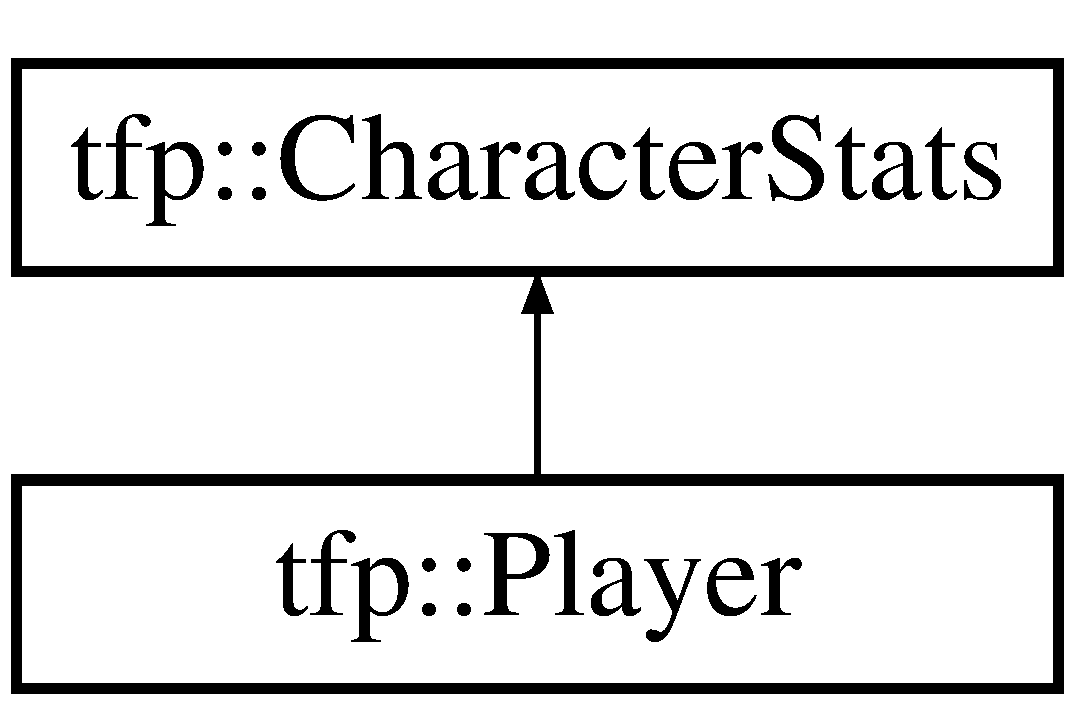
\includegraphics[height=2.000000cm]{classtfp_1_1_character_stats}
\end{center}
\end{figure}
\subsection*{Public Attributes}
\begin{DoxyCompactItemize}
\item 
\mbox{\Hypertarget{classtfp_1_1_character_stats_a9084ddc35e7df706a3a0c9fa5d17683c}\label{classtfp_1_1_character_stats_a9084ddc35e7df706a3a0c9fa5d17683c}} 
int \mbox{\hyperlink{classtfp_1_1_character_stats_a9084ddc35e7df706a3a0c9fa5d17683c}{Minimum\+Damage}}
\begin{DoxyCompactList}\small\item\em Podstawowe. \end{DoxyCompactList}\item 
\mbox{\Hypertarget{classtfp_1_1_character_stats_ae7171947f09e7d88e5c7e300839d319c}\label{classtfp_1_1_character_stats_ae7171947f09e7d88e5c7e300839d319c}} 
int {\bfseries Maximum\+Damage}
\item 
\mbox{\Hypertarget{classtfp_1_1_character_stats_ae4340d3ff6685ae764ba3dcf2629e883}\label{classtfp_1_1_character_stats_ae4340d3ff6685ae764ba3dcf2629e883}} 
int {\bfseries Strenght}
\item 
\mbox{\Hypertarget{classtfp_1_1_character_stats_a6242fbc2863be6959d9dd5ec459562af}\label{classtfp_1_1_character_stats_a6242fbc2863be6959d9dd5ec459562af}} 
int {\bfseries Vitality}
\item 
\mbox{\Hypertarget{classtfp_1_1_character_stats_af9b3f77488d5d4d7cd79dc6d74fa59e5}\label{classtfp_1_1_character_stats_af9b3f77488d5d4d7cd79dc6d74fa59e5}} 
int {\bfseries Dexterity}
\item 
\mbox{\Hypertarget{classtfp_1_1_character_stats_a8fb6030a1bdc0f5e6f7a40958976158d}\label{classtfp_1_1_character_stats_a8fb6030a1bdc0f5e6f7a40958976158d}} 
int {\bfseries Intelligence}
\item 
\mbox{\Hypertarget{classtfp_1_1_character_stats_a201f78d52c9132631ca49ff2b70df694}\label{classtfp_1_1_character_stats_a201f78d52c9132631ca49ff2b70df694}} 
float {\bfseries Attack\+Speed}
\item 
\mbox{\Hypertarget{classtfp_1_1_character_stats_ad5c8dbbc0c4328fba92d2df1cff18af8}\label{classtfp_1_1_character_stats_ad5c8dbbc0c4328fba92d2df1cff18af8}} 
float {\bfseries Movement\+Speed}
\item 
\mbox{\Hypertarget{classtfp_1_1_character_stats_a5affcf5a1191bded765ce2d3cb7cdc5c}\label{classtfp_1_1_character_stats_a5affcf5a1191bded765ce2d3cb7cdc5c}} 
float {\bfseries Life\+Steal}
\item 
\mbox{\Hypertarget{classtfp_1_1_character_stats_ae97b45a4fdc573b9c0f3154335da9efd}\label{classtfp_1_1_character_stats_ae97b45a4fdc573b9c0f3154335da9efd}} 
int \mbox{\hyperlink{classtfp_1_1_character_stats_ae97b45a4fdc573b9c0f3154335da9efd}{Ice\+Element}}
\begin{DoxyCompactList}\small\item\em Elementy. \end{DoxyCompactList}\item 
\mbox{\Hypertarget{classtfp_1_1_character_stats_a19ccc70a3ad3d84159a0efb3fc4bba05}\label{classtfp_1_1_character_stats_a19ccc70a3ad3d84159a0efb3fc4bba05}} 
int {\bfseries Darkness\+Element}
\item 
\mbox{\Hypertarget{classtfp_1_1_character_stats_ad8501dcb263619c49315cf6c1f091825}\label{classtfp_1_1_character_stats_ad8501dcb263619c49315cf6c1f091825}} 
int {\bfseries Fire\+Element}
\item 
\mbox{\Hypertarget{classtfp_1_1_character_stats_ab2ff404f8e5b8aab197acb3e401155bf}\label{classtfp_1_1_character_stats_ab2ff404f8e5b8aab197acb3e401155bf}} 
int {\bfseries Water\+Element}
\item 
\mbox{\Hypertarget{classtfp_1_1_character_stats_aeffe8b1ca891acd6fe8b81a1be9aaafa}\label{classtfp_1_1_character_stats_aeffe8b1ca891acd6fe8b81a1be9aaafa}} 
int {\bfseries Light\+Element}
\item 
\mbox{\Hypertarget{classtfp_1_1_character_stats_a31252ccf17f7fe0952f6296a5233d2a9}\label{classtfp_1_1_character_stats_a31252ccf17f7fe0952f6296a5233d2a9}} 
int {\bfseries Earth\+Element}
\item 
\mbox{\Hypertarget{classtfp_1_1_character_stats_ac002b63572e064781e92007bdf22ead3}\label{classtfp_1_1_character_stats_ac002b63572e064781e92007bdf22ead3}} 
int \mbox{\hyperlink{classtfp_1_1_character_stats_ac002b63572e064781e92007bdf22ead3}{Ice\+Resistance}}
\begin{DoxyCompactList}\small\item\em Resy. \end{DoxyCompactList}\item 
\mbox{\Hypertarget{classtfp_1_1_character_stats_a017c5848e4a15d4dacce824f2035c5fe}\label{classtfp_1_1_character_stats_a017c5848e4a15d4dacce824f2035c5fe}} 
int {\bfseries Darkness\+Resistance}
\item 
\mbox{\Hypertarget{classtfp_1_1_character_stats_a75935ab08be1cca4d184074d34ded6c8}\label{classtfp_1_1_character_stats_a75935ab08be1cca4d184074d34ded6c8}} 
int {\bfseries Fire\+Resistance}
\item 
\mbox{\Hypertarget{classtfp_1_1_character_stats_a27446f202901ac013c41c1d84f4e148a}\label{classtfp_1_1_character_stats_a27446f202901ac013c41c1d84f4e148a}} 
int {\bfseries Water\+Resistance}
\item 
\mbox{\Hypertarget{classtfp_1_1_character_stats_a22e81c081bc0bc319db4cacb3008d2ae}\label{classtfp_1_1_character_stats_a22e81c081bc0bc319db4cacb3008d2ae}} 
int {\bfseries Light\+Resistance}
\item 
\mbox{\Hypertarget{classtfp_1_1_character_stats_a045ac10e9bd1295a14aa7c0ececd94ae}\label{classtfp_1_1_character_stats_a045ac10e9bd1295a14aa7c0ececd94ae}} 
int {\bfseries Earth\+Resistance}
\end{DoxyCompactItemize}


The documentation for this class was generated from the following file\+:\begin{DoxyCompactItemize}
\item 
character.\+hpp\end{DoxyCompactItemize}

\hypertarget{classtfp_1_1_clickable_area}{}\section{tfp\+:\+:Clickable\+Area Class Reference}
\label{classtfp_1_1_clickable_area}\index{tfp\+::\+Clickable\+Area@{tfp\+::\+Clickable\+Area}}
\subsection*{Public Member Functions}
\begin{DoxyCompactItemize}
\item 
\mbox{\Hypertarget{classtfp_1_1_clickable_area_a430e91404b609c35d883c2259ea34fdf}\label{classtfp_1_1_clickable_area_a430e91404b609c35d883c2259ea34fdf}} 
\mbox{\hyperlink{classtfp_1_1_clickable_area_a430e91404b609c35d883c2259ea34fdf}{Clickable\+Area}} ()
\begin{DoxyCompactList}\small\item\em Konstruktor. \end{DoxyCompactList}\item 
\mbox{\Hypertarget{classtfp_1_1_clickable_area_a7352d983d6b4847ba14dbf934154c578}\label{classtfp_1_1_clickable_area_a7352d983d6b4847ba14dbf934154c578}} 
\mbox{\hyperlink{classtfp_1_1_clickable_area_a7352d983d6b4847ba14dbf934154c578}{Clickable\+Area}} (\mbox{\hyperlink{classtfp_1_1_game}{tfp\+::\+Game}} $\ast$Handle, sf\+::\+Vector2f Position, sf\+::\+Vector2f Size, bool Relative\+Size)
\begin{DoxyCompactList}\small\item\em Konstruktor z parametrami. Jesli Handle = nullptr nalezy uzyc \mbox{\hyperlink{classtfp_1_1_clickable_area_ad2384603fab60ebb57c9f07d81885294}{Set\+Game\+Handle()}};. \end{DoxyCompactList}\item 
\mbox{\Hypertarget{classtfp_1_1_clickable_area_acfc318db2a45a07e8e8c31418aeceeca}\label{classtfp_1_1_clickable_area_acfc318db2a45a07e8e8c31418aeceeca}} 
\mbox{\hyperlink{classtfp_1_1_clickable_area_acfc318db2a45a07e8e8c31418aeceeca}{$\sim$\+Clickable\+Area}} ()
\begin{DoxyCompactList}\small\item\em Destruktor. \end{DoxyCompactList}\item 
\mbox{\Hypertarget{classtfp_1_1_clickable_area_ab642055e04ace78218510c42a97f0f01}\label{classtfp_1_1_clickable_area_ab642055e04ace78218510c42a97f0f01}} 
void \mbox{\hyperlink{classtfp_1_1_clickable_area_ab642055e04ace78218510c42a97f0f01}{Reset}} (\mbox{\hyperlink{classtfp_1_1_game}{tfp\+::\+Game}} $\ast$Handle, sf\+::\+Vector2f Position, sf\+::\+Vector2f Size, bool Relative\+Size)
\begin{DoxyCompactList}\small\item\em Resetuje rozmiar i pozycje. \end{DoxyCompactList}\item 
\mbox{\Hypertarget{classtfp_1_1_clickable_area_ad2384603fab60ebb57c9f07d81885294}\label{classtfp_1_1_clickable_area_ad2384603fab60ebb57c9f07d81885294}} 
void \mbox{\hyperlink{classtfp_1_1_clickable_area_ad2384603fab60ebb57c9f07d81885294}{Set\+Game\+Handle}} (\mbox{\hyperlink{classtfp_1_1_game}{tfp\+::\+Game}} $\ast$Handle)
\begin{DoxyCompactList}\small\item\em Jesli nie ma mozliwosci ustawienia w konstruktorze. \end{DoxyCompactList}\item 
void \mbox{\hyperlink{classtfp_1_1_clickable_area_afeeaa98f916febd990f3a382612c8e34}{Check\+Active\+System}} ()
\begin{DoxyCompactList}\small\item\em Tylko do Button\+Global\+List. Sprawdza czy obszar zostal aktywowany. \end{DoxyCompactList}\item 
\mbox{\Hypertarget{classtfp_1_1_clickable_area_a318bfa23da7f0dd58489219e38663c0a}\label{classtfp_1_1_clickable_area_a318bfa23da7f0dd58489219e38663c0a}} 
const bool \& \mbox{\hyperlink{classtfp_1_1_clickable_area_a318bfa23da7f0dd58489219e38663c0a}{Is\+Disabled}} () const
\begin{DoxyCompactList}\small\item\em Zwraca czy obszar jest zablokowany. \end{DoxyCompactList}\item 
\mbox{\Hypertarget{classtfp_1_1_clickable_area_a102396d3a1af3a9f969f463b8b4b02e6}\label{classtfp_1_1_clickable_area_a102396d3a1af3a9f969f463b8b4b02e6}} 
void \mbox{\hyperlink{classtfp_1_1_clickable_area_a102396d3a1af3a9f969f463b8b4b02e6}{Set\+Disabled}} (bool State)
\begin{DoxyCompactList}\small\item\em Wylacza dzialane obszaru. \end{DoxyCompactList}\item 
\mbox{\Hypertarget{classtfp_1_1_clickable_area_a8112c2b80c5f0c87064037c7e545c8c2}\label{classtfp_1_1_clickable_area_a8112c2b80c5f0c87064037c7e545c8c2}} 
void \mbox{\hyperlink{classtfp_1_1_clickable_area_a8112c2b80c5f0c87064037c7e545c8c2}{Move}} (sf\+::\+Vector2f Distance)
\begin{DoxyCompactList}\small\item\em Przesuwanie obszaru. \end{DoxyCompactList}\item 
\mbox{\Hypertarget{classtfp_1_1_clickable_area_a2331a669fbbaf2bc14b5931c89efd277}\label{classtfp_1_1_clickable_area_a2331a669fbbaf2bc14b5931c89efd277}} 
void \mbox{\hyperlink{classtfp_1_1_clickable_area_a2331a669fbbaf2bc14b5931c89efd277}{Set\+Position}} (sf\+::\+Vector2f Position)
\begin{DoxyCompactList}\small\item\em Ustawia pozycje obszaru. \end{DoxyCompactList}\item 
\mbox{\Hypertarget{classtfp_1_1_clickable_area_af118a1882b577a097728c615395b6cfd}\label{classtfp_1_1_clickable_area_af118a1882b577a097728c615395b6cfd}} 
void \mbox{\hyperlink{classtfp_1_1_clickable_area_af118a1882b577a097728c615395b6cfd}{Set\+Size}} (sf\+::\+Vector2f Size)
\begin{DoxyCompactList}\small\item\em Ustawia wymiary obszaru. \end{DoxyCompactList}\item 
\mbox{\Hypertarget{classtfp_1_1_clickable_area_a5f195520a56f10ffe940fe98215a7f9b}\label{classtfp_1_1_clickable_area_a5f195520a56f10ffe940fe98215a7f9b}} 
\mbox{\hyperlink{classtfp_1_1_game}{tfp\+::\+Game}} $\ast$ \mbox{\hyperlink{classtfp_1_1_clickable_area_a5f195520a56f10ffe940fe98215a7f9b}{Get\+Game\+Handle}} ()
\begin{DoxyCompactList}\small\item\em Zwraca uchwyt na gre. \end{DoxyCompactList}\item 
\mbox{\Hypertarget{classtfp_1_1_clickable_area_afdd473c2814b40ae47a6d64c08809cd7}\label{classtfp_1_1_clickable_area_afdd473c2814b40ae47a6d64c08809cd7}} 
bool \mbox{\hyperlink{classtfp_1_1_clickable_area_afdd473c2814b40ae47a6d64c08809cd7}{Is\+Button\+Down}} ()
\begin{DoxyCompactList}\small\item\em Zwraca czy jest wciskany. \end{DoxyCompactList}\item 
\mbox{\Hypertarget{classtfp_1_1_clickable_area_add58fcc4eca0a7c0c0d533e54e380f5b}\label{classtfp_1_1_clickable_area_add58fcc4eca0a7c0c0d533e54e380f5b}} 
bool \mbox{\hyperlink{classtfp_1_1_clickable_area_add58fcc4eca0a7c0c0d533e54e380f5b}{Is\+Button\+Pressed}} ()
\begin{DoxyCompactList}\small\item\em Zwraca czy jest nacisniety. \end{DoxyCompactList}\item 
\mbox{\Hypertarget{classtfp_1_1_clickable_area_a3fb5bb723bff9e60248f33721b04460e}\label{classtfp_1_1_clickable_area_a3fb5bb723bff9e60248f33721b04460e}} 
void \mbox{\hyperlink{classtfp_1_1_clickable_area_a3fb5bb723bff9e60248f33721b04460e}{Set\+Active}} (bool State)
\begin{DoxyCompactList}\small\item\em Ustawia obszar jako aktywny. \end{DoxyCompactList}\item 
\mbox{\Hypertarget{classtfp_1_1_clickable_area_a059b79306eb4aa372e515ae68e872b2b}\label{classtfp_1_1_clickable_area_a059b79306eb4aa372e515ae68e872b2b}} 
sf\+::\+Vector2f \& \mbox{\hyperlink{classtfp_1_1_clickable_area_a059b79306eb4aa372e515ae68e872b2b}{Get\+Position}} ()
\begin{DoxyCompactList}\small\item\em Zwraca pozycje area. \end{DoxyCompactList}\item 
\mbox{\Hypertarget{classtfp_1_1_clickable_area_a1acb675c98f351065e33a248cd6893ed}\label{classtfp_1_1_clickable_area_a1acb675c98f351065e33a248cd6893ed}} 
sf\+::\+Vector2f \& \mbox{\hyperlink{classtfp_1_1_clickable_area_a1acb675c98f351065e33a248cd6893ed}{Get\+Size}} ()
\begin{DoxyCompactList}\small\item\em Zwraca rozmiar area. \end{DoxyCompactList}\end{DoxyCompactItemize}


\subsection{Member Function Documentation}
\mbox{\Hypertarget{classtfp_1_1_clickable_area_afeeaa98f916febd990f3a382612c8e34}\label{classtfp_1_1_clickable_area_afeeaa98f916febd990f3a382612c8e34}} 
\index{tfp\+::\+Clickable\+Area@{tfp\+::\+Clickable\+Area}!Check\+Active\+System@{Check\+Active\+System}}
\index{Check\+Active\+System@{Check\+Active\+System}!tfp\+::\+Clickable\+Area@{tfp\+::\+Clickable\+Area}}
\subsubsection{\texorpdfstring{Check\+Active\+System()}{CheckActiveSystem()}}
{\footnotesize\ttfamily void tfp\+::\+Clickable\+Area\+::\+Check\+Active\+System (\begin{DoxyParamCaption}{ }\end{DoxyParamCaption})}



Tylko do Button\+Global\+List. Sprawdza czy obszar zostal aktywowany. 

Klikniecie w przycisk

Left\+Button\+Up in rect

Left\+Button\+Up outside rect

Klikniecie w przycisk

Left\+Button\+Up in rect

Left\+Button\+Up outside rect 

The documentation for this class was generated from the following files\+:\begin{DoxyCompactItemize}
\item 
area.\+hpp\item 
area.\+cpp\end{DoxyCompactItemize}

\hypertarget{classtfp_1_1_clock_class}{}\section{tfp\+:\+:Clock\+Class Class Reference}
\label{classtfp_1_1_clock_class}\index{tfp\+::\+Clock\+Class@{tfp\+::\+Clock\+Class}}
\subsection*{Public Member Functions}
\begin{DoxyCompactItemize}
\item 
\mbox{\Hypertarget{classtfp_1_1_clock_class_adde3feaf78998365d896233c55ee7afa}\label{classtfp_1_1_clock_class_adde3feaf78998365d896233c55ee7afa}} 
\mbox{\hyperlink{classtfp_1_1_clock_class_adde3feaf78998365d896233c55ee7afa}{Clock\+Class}} ()
\begin{DoxyCompactList}\small\item\em Konstruktor. \end{DoxyCompactList}\item 
\mbox{\Hypertarget{classtfp_1_1_clock_class_abfb7964af48bf2a5bc7a99025b47f798}\label{classtfp_1_1_clock_class_abfb7964af48bf2a5bc7a99025b47f798}} 
\mbox{\hyperlink{classtfp_1_1_clock_class_abfb7964af48bf2a5bc7a99025b47f798}{$\sim$\+Clock\+Class}} ()
\begin{DoxyCompactList}\small\item\em Destruktor. \end{DoxyCompactList}\item 
\mbox{\Hypertarget{classtfp_1_1_clock_class_a1ab26448019bb72f368ce49d5db8f743}\label{classtfp_1_1_clock_class_a1ab26448019bb72f368ce49d5db8f743}} 
void \mbox{\hyperlink{classtfp_1_1_clock_class_a1ab26448019bb72f368ce49d5db8f743}{Restart}} ()
\begin{DoxyCompactList}\small\item\em Restartuje zegar. \end{DoxyCompactList}\item 
\mbox{\Hypertarget{classtfp_1_1_clock_class_a2d29510591ec634222b118aa2ef598f2}\label{classtfp_1_1_clock_class_a2d29510591ec634222b118aa2ef598f2}} 
const float \mbox{\hyperlink{classtfp_1_1_clock_class_a2d29510591ec634222b118aa2ef598f2}{Get\+Delta\+Time}} () const
\begin{DoxyCompactList}\small\item\em Zwraca miniony czas w sekundach. \end{DoxyCompactList}\end{DoxyCompactItemize}


The documentation for this class was generated from the following files\+:\begin{DoxyCompactItemize}
\item 
clock.\+hpp\item 
clock.\+cpp\end{DoxyCompactItemize}

\hypertarget{classtfp_1_1_command_block}{}\section{tfp\+:\+:Command\+Block Class Reference}
\label{classtfp_1_1_command_block}\index{tfp\+::\+Command\+Block@{tfp\+::\+Command\+Block}}
\subsection*{Public Member Functions}
\begin{DoxyCompactItemize}
\item 
\mbox{\Hypertarget{classtfp_1_1_command_block_a153df72580c2a88ff78c8bbf54e3930a}\label{classtfp_1_1_command_block_a153df72580c2a88ff78c8bbf54e3930a}} 
\mbox{\hyperlink{classtfp_1_1_command_block_a153df72580c2a88ff78c8bbf54e3930a}{Command\+Block}} ()
\begin{DoxyCompactList}\small\item\em Konstruktor. \end{DoxyCompactList}\item 
\mbox{\Hypertarget{classtfp_1_1_command_block_a6236bd155b13d4233688958377ca82fe}\label{classtfp_1_1_command_block_a6236bd155b13d4233688958377ca82fe}} 
\mbox{\hyperlink{classtfp_1_1_command_block_a6236bd155b13d4233688958377ca82fe}{$\sim$\+Command\+Block}} ()
\begin{DoxyCompactList}\small\item\em Destruktor. \end{DoxyCompactList}\item 
\mbox{\Hypertarget{classtfp_1_1_command_block_af4459526fcd977acf5f7b0805042a6ad}\label{classtfp_1_1_command_block_af4459526fcd977acf5f7b0805042a6ad}} 
void \mbox{\hyperlink{classtfp_1_1_command_block_af4459526fcd977acf5f7b0805042a6ad}{Set\+Game\+Handle}} (\mbox{\hyperlink{classtfp_1_1_game}{tfp\+::\+Game}} $\ast$Handle)
\begin{DoxyCompactList}\small\item\em Ustawia wskaznik na gre ktora obsluguje. \end{DoxyCompactList}\item 
void \mbox{\hyperlink{classtfp_1_1_command_block_ab87816104ea217209676d5e6788921a1}{Run\+Command}} (std\+::string Command)
\begin{DoxyCompactList}\small\item\em Wykonuje podana komende. \end{DoxyCompactList}\item 
\mbox{\Hypertarget{classtfp_1_1_command_block_a84298fbd9c4515d4c4fd4cb6c2bc4320}\label{classtfp_1_1_command_block_a84298fbd9c4515d4c4fd4cb6c2bc4320}} 
std\+::string \mbox{\hyperlink{classtfp_1_1_command_block_a84298fbd9c4515d4c4fd4cb6c2bc4320}{Get\+Game\+Manager\+Command}} ()
\begin{DoxyCompactList}\small\item\em Zwraca komende dla menedzera gier. \end{DoxyCompactList}\item 
\mbox{\Hypertarget{classtfp_1_1_command_block_ad7b89f3ab84cbf4ce59e39bb499ed95b}\label{classtfp_1_1_command_block_ad7b89f3ab84cbf4ce59e39bb499ed95b}} 
const bool \mbox{\hyperlink{classtfp_1_1_command_block_ad7b89f3ab84cbf4ce59e39bb499ed95b}{Is\+Game\+Manager\+Command\+List\+Empty}} () const
\begin{DoxyCompactList}\small\item\em Zwraca czy lista komend dla menedzera jest pusta. \end{DoxyCompactList}\end{DoxyCompactItemize}


\subsection{Member Function Documentation}
\mbox{\Hypertarget{classtfp_1_1_command_block_ab87816104ea217209676d5e6788921a1}\label{classtfp_1_1_command_block_ab87816104ea217209676d5e6788921a1}} 
\index{tfp\+::\+Command\+Block@{tfp\+::\+Command\+Block}!Run\+Command@{Run\+Command}}
\index{Run\+Command@{Run\+Command}!tfp\+::\+Command\+Block@{tfp\+::\+Command\+Block}}
\subsubsection{\texorpdfstring{Run\+Command()}{RunCommand()}}
{\footnotesize\ttfamily void tfp\+::\+Command\+Block\+::\+Run\+Command (\begin{DoxyParamCaption}\item[{std\+::string}]{Command }\end{DoxyParamCaption})}



Wykonuje podana komende. 

Macrodefinitions

Commands

Rodzaje

Unlisted commands 

The documentation for this class was generated from the following files\+:\begin{DoxyCompactItemize}
\item 
commandblock.\+hpp\item 
commandblock.\+cpp\end{DoxyCompactItemize}

\hypertarget{classtfp_1_1_debug_class}{}\section{tfp\+:\+:Debug\+Class Class Reference}
\label{classtfp_1_1_debug_class}\index{tfp\+::\+Debug\+Class@{tfp\+::\+Debug\+Class}}
\subsection*{Public Member Functions}
\begin{DoxyCompactItemize}
\item 
\mbox{\Hypertarget{classtfp_1_1_debug_class_a504eef6b38440a5ab98d1b44a22c5b7d}\label{classtfp_1_1_debug_class_a504eef6b38440a5ab98d1b44a22c5b7d}} 
void \mbox{\hyperlink{classtfp_1_1_debug_class_a504eef6b38440a5ab98d1b44a22c5b7d}{Error}} (std\+::string Message)
\begin{DoxyCompactList}\small\item\em Wiadomosc o bledzie. \end{DoxyCompactList}\item 
\mbox{\Hypertarget{classtfp_1_1_debug_class_ae0a7705a4594cec104ebea2300881551}\label{classtfp_1_1_debug_class_ae0a7705a4594cec104ebea2300881551}} 
void \mbox{\hyperlink{classtfp_1_1_debug_class_ae0a7705a4594cec104ebea2300881551}{Info}} (std\+::string Message)
\begin{DoxyCompactList}\small\item\em Informacja do testow. \end{DoxyCompactList}\item 
\mbox{\Hypertarget{classtfp_1_1_debug_class_a44446f2e6062113d16ee1c9c8bb4e812}\label{classtfp_1_1_debug_class_a44446f2e6062113d16ee1c9c8bb4e812}} 
void \mbox{\hyperlink{classtfp_1_1_debug_class_a44446f2e6062113d16ee1c9c8bb4e812}{Warning}} (std\+::string Message)
\begin{DoxyCompactList}\small\item\em Wiadomosc o ostrzezeniu. \end{DoxyCompactList}\item 
\mbox{\Hypertarget{classtfp_1_1_debug_class_abfe06ba8dd78d2e8430325c70c1fa32e}\label{classtfp_1_1_debug_class_abfe06ba8dd78d2e8430325c70c1fa32e}} 
void \mbox{\hyperlink{classtfp_1_1_debug_class_abfe06ba8dd78d2e8430325c70c1fa32e}{Command}} (std\+::string Message)
\begin{DoxyCompactList}\small\item\em Wiadomosc o uzytej komendzie. \end{DoxyCompactList}\item 
\mbox{\Hypertarget{classtfp_1_1_debug_class_a01b47eb735ae9a2309df1095321e4776}\label{classtfp_1_1_debug_class_a01b47eb735ae9a2309df1095321e4776}} 
void \mbox{\hyperlink{classtfp_1_1_debug_class_a01b47eb735ae9a2309df1095321e4776}{Log}} (std\+::string Text)
\begin{DoxyCompactList}\small\item\em Zapisuje wiadomosc do logu. \end{DoxyCompactList}\item 
\mbox{\Hypertarget{classtfp_1_1_debug_class_ab0f6da60a7cb6b8840f6249206d03d8c}\label{classtfp_1_1_debug_class_ab0f6da60a7cb6b8840f6249206d03d8c}} 
void \mbox{\hyperlink{classtfp_1_1_debug_class_ab0f6da60a7cb6b8840f6249206d03d8c}{Add\+To\+History}} (std\+::string Text)
\begin{DoxyCompactList}\small\item\em Dodaje wiadomosc do historii. \end{DoxyCompactList}\item 
\mbox{\Hypertarget{classtfp_1_1_debug_class_aad5bf085bdaf254997dfe45cb4557f2b}\label{classtfp_1_1_debug_class_aad5bf085bdaf254997dfe45cb4557f2b}} 
std\+::string \mbox{\hyperlink{classtfp_1_1_debug_class_aad5bf085bdaf254997dfe45cb4557f2b}{Get\+Debug\+Message}} (int Number)
\begin{DoxyCompactList}\small\item\em Zwraca wiadomisc o numerze. \end{DoxyCompactList}\item 
\mbox{\Hypertarget{classtfp_1_1_debug_class_a5d7c1e5c227fbf1a189c797c772a73cc}\label{classtfp_1_1_debug_class_a5d7c1e5c227fbf1a189c797c772a73cc}} 
const bool \mbox{\hyperlink{classtfp_1_1_debug_class_a5d7c1e5c227fbf1a189c797c772a73cc}{Is\+Debug\+Message\+Availiable}} (int Number)
\begin{DoxyCompactList}\small\item\em Zwraca czy dany numer wiadomosci jest dostepny. \end{DoxyCompactList}\item 
\mbox{\Hypertarget{classtfp_1_1_debug_class_a06f935f8abee02e5633fc26e6b0b380e}\label{classtfp_1_1_debug_class_a06f935f8abee02e5633fc26e6b0b380e}} 
int \mbox{\hyperlink{classtfp_1_1_debug_class_a06f935f8abee02e5633fc26e6b0b380e}{What\+Is\+The\+Lowest\+Debug\+Message\+Number}} ()
\begin{DoxyCompactList}\small\item\em Zwraca najnizszsy numer wiadomosci. \end{DoxyCompactList}\item 
\mbox{\Hypertarget{classtfp_1_1_debug_class_a5d24ffb7e8f56955fcc00672186f0615}\label{classtfp_1_1_debug_class_a5d24ffb7e8f56955fcc00672186f0615}} 
\mbox{\hyperlink{classtfp_1_1_debug_class_a5d24ffb7e8f56955fcc00672186f0615}{Debug\+Class}} ()
\begin{DoxyCompactList}\small\item\em Konstruktor. \end{DoxyCompactList}\item 
\mbox{\Hypertarget{classtfp_1_1_debug_class_aa475e7cd69f8f9ee8e20a2539aa5ea1c}\label{classtfp_1_1_debug_class_aa475e7cd69f8f9ee8e20a2539aa5ea1c}} 
\mbox{\hyperlink{classtfp_1_1_debug_class_aa475e7cd69f8f9ee8e20a2539aa5ea1c}{$\sim$\+Debug\+Class}} ()
\begin{DoxyCompactList}\small\item\em Destruktor. \end{DoxyCompactList}\end{DoxyCompactItemize}


The documentation for this class was generated from the following files\+:\begin{DoxyCompactItemize}
\item 
debug.\+hpp\item 
debug.\+cpp\end{DoxyCompactItemize}

\hypertarget{classtfp_1_1_dragable_area}{}\section{tfp\+:\+:Dragable\+Area Class Reference}
\label{classtfp_1_1_dragable_area}\index{tfp\+::\+Dragable\+Area@{tfp\+::\+Dragable\+Area}}
\subsection*{Public Member Functions}
\begin{DoxyCompactItemize}
\item 
\mbox{\Hypertarget{classtfp_1_1_dragable_area_a45f053c1097a1b98d077b155e19840e0}\label{classtfp_1_1_dragable_area_a45f053c1097a1b98d077b155e19840e0}} 
\mbox{\hyperlink{classtfp_1_1_dragable_area_a45f053c1097a1b98d077b155e19840e0}{Dragable\+Area}} ()
\begin{DoxyCompactList}\small\item\em Konstruktor bez parametru wymaga uzycia funkcji \mbox{\hyperlink{classtfp_1_1_dragable_area_a3142a5b247faf918af0b2bbc557707db}{Reset()}} \end{DoxyCompactList}\item 
\mbox{\Hypertarget{classtfp_1_1_dragable_area_a093621d902ca03b14c499d7d3b9a45ac}\label{classtfp_1_1_dragable_area_a093621d902ca03b14c499d7d3b9a45ac}} 
\mbox{\hyperlink{classtfp_1_1_dragable_area_a093621d902ca03b14c499d7d3b9a45ac}{Dragable\+Area}} (\mbox{\hyperlink{classtfp_1_1_game}{tfp\+::\+Game}} $\ast$Handle, sf\+::\+Vector2f Position, sf\+::\+Vector2f Size, bool Relative\+Size)
\begin{DoxyCompactList}\small\item\em Konstruktor z parametrami. Jesli Handle = nullptr nalezy uzyc \mbox{\hyperlink{classtfp_1_1_dragable_area_a8b699f79826c5225ffe3e58e2ebda12a}{Set\+Game\+Handle()}};. \end{DoxyCompactList}\item 
\mbox{\Hypertarget{classtfp_1_1_dragable_area_ade01cf321c7f81ce585addb89ed06919}\label{classtfp_1_1_dragable_area_ade01cf321c7f81ce585addb89ed06919}} 
\mbox{\hyperlink{classtfp_1_1_dragable_area_ade01cf321c7f81ce585addb89ed06919}{$\sim$\+Dragable\+Area}} ()
\begin{DoxyCompactList}\small\item\em Destruktor. \end{DoxyCompactList}\item 
\mbox{\Hypertarget{classtfp_1_1_dragable_area_a3142a5b247faf918af0b2bbc557707db}\label{classtfp_1_1_dragable_area_a3142a5b247faf918af0b2bbc557707db}} 
void \mbox{\hyperlink{classtfp_1_1_dragable_area_a3142a5b247faf918af0b2bbc557707db}{Reset}} (\mbox{\hyperlink{classtfp_1_1_game}{tfp\+::\+Game}} $\ast$Handle, sf\+::\+Vector2f Position, sf\+::\+Vector2f Size, bool Relative\+Size)
\begin{DoxyCompactList}\small\item\em Resetuje rozmiar i pozycje. \end{DoxyCompactList}\item 
\mbox{\Hypertarget{classtfp_1_1_dragable_area_a1cd099aa0da737d1497e15d65c215ff6}\label{classtfp_1_1_dragable_area_a1cd099aa0da737d1497e15d65c215ff6}} 
void \mbox{\hyperlink{classtfp_1_1_dragable_area_a1cd099aa0da737d1497e15d65c215ff6}{Check\+Active\+System}} ()
\begin{DoxyCompactList}\small\item\em Tylko do Button\+Global\+List. Sprawdza czy obszar zostal aktywowany. \end{DoxyCompactList}\item 
\mbox{\Hypertarget{classtfp_1_1_dragable_area_a8d768756ed7fe3184e54c53967c6b6da}\label{classtfp_1_1_dragable_area_a8d768756ed7fe3184e54c53967c6b6da}} 
const bool \mbox{\hyperlink{classtfp_1_1_dragable_area_a8d768756ed7fe3184e54c53967c6b6da}{Is\+Active}} () const
\begin{DoxyCompactList}\small\item\em Zwraca czy obszar jest aktywny. \end{DoxyCompactList}\item 
\mbox{\Hypertarget{classtfp_1_1_dragable_area_a49875c6c9c67aced70cbdf5e5b2cec75}\label{classtfp_1_1_dragable_area_a49875c6c9c67aced70cbdf5e5b2cec75}} 
const bool \& \mbox{\hyperlink{classtfp_1_1_dragable_area_a49875c6c9c67aced70cbdf5e5b2cec75}{Is\+Disabled}} () const
\begin{DoxyCompactList}\small\item\em Zwraca czy obszar jest zablokowany. \end{DoxyCompactList}\item 
\mbox{\Hypertarget{classtfp_1_1_dragable_area_a94fb0516e10190084215ab8db4d37b61}\label{classtfp_1_1_dragable_area_a94fb0516e10190084215ab8db4d37b61}} 
void \mbox{\hyperlink{classtfp_1_1_dragable_area_a94fb0516e10190084215ab8db4d37b61}{Set\+Active}} (bool State)
\begin{DoxyCompactList}\small\item\em Ustawia obszar jako aktywny. \end{DoxyCompactList}\item 
\mbox{\Hypertarget{classtfp_1_1_dragable_area_a1890d67de00cadb22cf64b8960f65eb4}\label{classtfp_1_1_dragable_area_a1890d67de00cadb22cf64b8960f65eb4}} 
void \mbox{\hyperlink{classtfp_1_1_dragable_area_a1890d67de00cadb22cf64b8960f65eb4}{Set\+Disabled}} (bool State)
\begin{DoxyCompactList}\small\item\em Wylacza dzialane obszaru. \end{DoxyCompactList}\item 
\mbox{\Hypertarget{classtfp_1_1_dragable_area_a8b699f79826c5225ffe3e58e2ebda12a}\label{classtfp_1_1_dragable_area_a8b699f79826c5225ffe3e58e2ebda12a}} 
void \mbox{\hyperlink{classtfp_1_1_dragable_area_a8b699f79826c5225ffe3e58e2ebda12a}{Set\+Game\+Handle}} (\mbox{\hyperlink{classtfp_1_1_game}{tfp\+::\+Game}} $\ast$Handle)
\begin{DoxyCompactList}\small\item\em Dragable. \end{DoxyCompactList}\item 
\mbox{\Hypertarget{classtfp_1_1_dragable_area_accb4f33f1ce170e33fcc35dcece72963}\label{classtfp_1_1_dragable_area_accb4f33f1ce170e33fcc35dcece72963}} 
void \mbox{\hyperlink{classtfp_1_1_dragable_area_accb4f33f1ce170e33fcc35dcece72963}{Move}} (sf\+::\+Vector2f Distance)
\begin{DoxyCompactList}\small\item\em Przesuwanie obszaru. \end{DoxyCompactList}\item 
\mbox{\Hypertarget{classtfp_1_1_dragable_area_a03f05c8bdfbb80d53ecb1f437e52ea04}\label{classtfp_1_1_dragable_area_a03f05c8bdfbb80d53ecb1f437e52ea04}} 
void \mbox{\hyperlink{classtfp_1_1_dragable_area_a03f05c8bdfbb80d53ecb1f437e52ea04}{Set\+Position}} (sf\+::\+Vector2f Position)
\begin{DoxyCompactList}\small\item\em Ustawia pozycje obszaru. \end{DoxyCompactList}\item 
\mbox{\Hypertarget{classtfp_1_1_dragable_area_a3bf6adac8b6c43d2cb0d20a5bae34bc7}\label{classtfp_1_1_dragable_area_a3bf6adac8b6c43d2cb0d20a5bae34bc7}} 
\mbox{\hyperlink{classtfp_1_1_game}{tfp\+::\+Game}} $\ast$ \mbox{\hyperlink{classtfp_1_1_dragable_area_a3bf6adac8b6c43d2cb0d20a5bae34bc7}{Get\+Game\+Handle}} ()
\begin{DoxyCompactList}\small\item\em Zwraca uchwyt na gre. \end{DoxyCompactList}\item 
\mbox{\Hypertarget{classtfp_1_1_dragable_area_ab6c1e015b34271a22cef709bb8041218}\label{classtfp_1_1_dragable_area_ab6c1e015b34271a22cef709bb8041218}} 
sf\+::\+Vector2f \& \mbox{\hyperlink{classtfp_1_1_dragable_area_ab6c1e015b34271a22cef709bb8041218}{Get\+Position}} ()
\begin{DoxyCompactList}\small\item\em Zwraca pozycje area. \end{DoxyCompactList}\item 
\mbox{\Hypertarget{classtfp_1_1_dragable_area_a7f936c9b861f023899adf8bf5b0a8cb8}\label{classtfp_1_1_dragable_area_a7f936c9b861f023899adf8bf5b0a8cb8}} 
sf\+::\+Vector2f \& \mbox{\hyperlink{classtfp_1_1_dragable_area_a7f936c9b861f023899adf8bf5b0a8cb8}{Get\+Size}} ()
\begin{DoxyCompactList}\small\item\em Zwraca rozmiar area. \end{DoxyCompactList}\end{DoxyCompactItemize}


The documentation for this class was generated from the following files\+:\begin{DoxyCompactItemize}
\item 
area.\+hpp\item 
area.\+cpp\end{DoxyCompactItemize}

\hypertarget{classrapidxml_1_1file}{}\section{rapidxml\+:\+:file$<$ Ch $>$ Class Template Reference}
\label{classrapidxml_1_1file}\index{rapidxml\+::file$<$ Ch $>$@{rapidxml\+::file$<$ Ch $>$}}


Represents data loaded from a file.  




{\ttfamily \#include $<$rapidxml\+\_\+utils.\+hpp$>$}

\subsection*{Public Member Functions}
\begin{DoxyCompactItemize}
\item 
\mbox{\hyperlink{classrapidxml_1_1file_ae881a3cab1fe7152d45c92a8d7606cb3}{file}} (const char $\ast$filename)
\item 
\mbox{\hyperlink{classrapidxml_1_1file_a90707ccd991cc392dcf4bef37eed9d1f}{file}} (std\+::basic\+\_\+istream$<$ Ch $>$ \&stream)
\item 
Ch $\ast$ \mbox{\hyperlink{classrapidxml_1_1file_af1c71d65862c7af14e4708e32a80c1de}{data}} ()
\item 
const Ch $\ast$ \mbox{\hyperlink{classrapidxml_1_1file_a044bdd99e59157b8a5a1b28c2f32da4d}{data}} () const
\item 
std\+::size\+\_\+t \mbox{\hyperlink{classrapidxml_1_1file_aacd451b3def3ad056fe8342dccee35cd}{size}} () const
\end{DoxyCompactItemize}


\subsection{Detailed Description}
\subsubsection*{template$<$class Ch = char$>$\newline
class rapidxml\+::file$<$ Ch $>$}

Represents data loaded from a file. 

\subsection{Constructor \& Destructor Documentation}
\mbox{\Hypertarget{classrapidxml_1_1file_ae881a3cab1fe7152d45c92a8d7606cb3}\label{classrapidxml_1_1file_ae881a3cab1fe7152d45c92a8d7606cb3}} 
\index{rapidxml\+::file@{rapidxml\+::file}!file@{file}}
\index{file@{file}!rapidxml\+::file@{rapidxml\+::file}}
\subsubsection{\texorpdfstring{file()}{file()}\hspace{0.1cm}{\footnotesize\ttfamily [1/2]}}
{\footnotesize\ttfamily template$<$class Ch  = char$>$ \\
\mbox{\hyperlink{classrapidxml_1_1file}{rapidxml\+::file}}$<$ Ch $>$\+::\mbox{\hyperlink{classrapidxml_1_1file}{file}} (\begin{DoxyParamCaption}\item[{const char $\ast$}]{filename }\end{DoxyParamCaption})\hspace{0.3cm}{\ttfamily [inline]}}

Loads file into the memory. Data will be automatically destroyed by the destructor. 
\begin{DoxyParams}{Parameters}
{\em filename} & Filename to load. \\
\hline
\end{DoxyParams}
\mbox{\Hypertarget{classrapidxml_1_1file_a90707ccd991cc392dcf4bef37eed9d1f}\label{classrapidxml_1_1file_a90707ccd991cc392dcf4bef37eed9d1f}} 
\index{rapidxml\+::file@{rapidxml\+::file}!file@{file}}
\index{file@{file}!rapidxml\+::file@{rapidxml\+::file}}
\subsubsection{\texorpdfstring{file()}{file()}\hspace{0.1cm}{\footnotesize\ttfamily [2/2]}}
{\footnotesize\ttfamily template$<$class Ch  = char$>$ \\
\mbox{\hyperlink{classrapidxml_1_1file}{rapidxml\+::file}}$<$ Ch $>$\+::\mbox{\hyperlink{classrapidxml_1_1file}{file}} (\begin{DoxyParamCaption}\item[{std\+::basic\+\_\+istream$<$ Ch $>$ \&}]{stream }\end{DoxyParamCaption})\hspace{0.3cm}{\ttfamily [inline]}}

Loads file into the memory. Data will be automatically destroyed by the destructor 
\begin{DoxyParams}{Parameters}
{\em stream} & Stream to load from \\
\hline
\end{DoxyParams}


\subsection{Member Function Documentation}
\mbox{\Hypertarget{classrapidxml_1_1file_af1c71d65862c7af14e4708e32a80c1de}\label{classrapidxml_1_1file_af1c71d65862c7af14e4708e32a80c1de}} 
\index{rapidxml\+::file@{rapidxml\+::file}!data@{data}}
\index{data@{data}!rapidxml\+::file@{rapidxml\+::file}}
\subsubsection{\texorpdfstring{data()}{data()}\hspace{0.1cm}{\footnotesize\ttfamily [1/2]}}
{\footnotesize\ttfamily template$<$class Ch  = char$>$ \\
Ch$\ast$ \mbox{\hyperlink{classrapidxml_1_1file}{rapidxml\+::file}}$<$ Ch $>$\+::data (\begin{DoxyParamCaption}{ }\end{DoxyParamCaption})\hspace{0.3cm}{\ttfamily [inline]}}

Gets file data. \begin{DoxyReturn}{Returns}
Pointer to data of file. 
\end{DoxyReturn}
\mbox{\Hypertarget{classrapidxml_1_1file_a044bdd99e59157b8a5a1b28c2f32da4d}\label{classrapidxml_1_1file_a044bdd99e59157b8a5a1b28c2f32da4d}} 
\index{rapidxml\+::file@{rapidxml\+::file}!data@{data}}
\index{data@{data}!rapidxml\+::file@{rapidxml\+::file}}
\subsubsection{\texorpdfstring{data()}{data()}\hspace{0.1cm}{\footnotesize\ttfamily [2/2]}}
{\footnotesize\ttfamily template$<$class Ch  = char$>$ \\
const Ch$\ast$ \mbox{\hyperlink{classrapidxml_1_1file}{rapidxml\+::file}}$<$ Ch $>$\+::data (\begin{DoxyParamCaption}{ }\end{DoxyParamCaption}) const\hspace{0.3cm}{\ttfamily [inline]}}

Gets file data. \begin{DoxyReturn}{Returns}
Pointer to data of file. 
\end{DoxyReturn}
\mbox{\Hypertarget{classrapidxml_1_1file_aacd451b3def3ad056fe8342dccee35cd}\label{classrapidxml_1_1file_aacd451b3def3ad056fe8342dccee35cd}} 
\index{rapidxml\+::file@{rapidxml\+::file}!size@{size}}
\index{size@{size}!rapidxml\+::file@{rapidxml\+::file}}
\subsubsection{\texorpdfstring{size()}{size()}}
{\footnotesize\ttfamily template$<$class Ch  = char$>$ \\
std\+::size\+\_\+t \mbox{\hyperlink{classrapidxml_1_1file}{rapidxml\+::file}}$<$ Ch $>$\+::size (\begin{DoxyParamCaption}{ }\end{DoxyParamCaption}) const\hspace{0.3cm}{\ttfamily [inline]}}

Gets file data size. \begin{DoxyReturn}{Returns}
Size of file data, in characters. 
\end{DoxyReturn}


The documentation for this class was generated from the following file\+:\begin{DoxyCompactItemize}
\item 
\mbox{\hyperlink{rapidxml__utils_8hpp}{rapidxml\+\_\+utils.\+hpp}}\end{DoxyCompactItemize}

\hypertarget{classtfp_1_1_focus_area}{}\section{tfp\+:\+:Focus\+Area Class Reference}
\label{classtfp_1_1_focus_area}\index{tfp\+::\+Focus\+Area@{tfp\+::\+Focus\+Area}}
\subsection*{Public Member Functions}
\begin{DoxyCompactItemize}
\item 
\mbox{\Hypertarget{classtfp_1_1_focus_area_af46f704ef1548e51e678e134f8f92ec5}\label{classtfp_1_1_focus_area_af46f704ef1548e51e678e134f8f92ec5}} 
\mbox{\hyperlink{classtfp_1_1_focus_area_af46f704ef1548e51e678e134f8f92ec5}{Focus\+Area}} ()
\begin{DoxyCompactList}\small\item\em Konstruktor bez parametru wymaga uzycia funkcji \mbox{\hyperlink{classtfp_1_1_focus_area_a23c05868f070600b214c113e3705b4c9}{Reset()}} \end{DoxyCompactList}\item 
\mbox{\Hypertarget{classtfp_1_1_focus_area_ad9989ba0ff51d9c07d7581b93714eb7f}\label{classtfp_1_1_focus_area_ad9989ba0ff51d9c07d7581b93714eb7f}} 
\mbox{\hyperlink{classtfp_1_1_focus_area_ad9989ba0ff51d9c07d7581b93714eb7f}{Focus\+Area}} (\mbox{\hyperlink{classtfp_1_1_game}{tfp\+::\+Game}} $\ast$Handle, sf\+::\+Vector2f Position, sf\+::\+Vector2f Size, bool Relative\+Size)
\begin{DoxyCompactList}\small\item\em Konstruktor z parametrami. Jesli Handle = nullptr nalezy uzyc Set\+Game\+Handle();. \end{DoxyCompactList}\item 
\mbox{\Hypertarget{classtfp_1_1_focus_area_a80671cf059958c45fe92d9878bbc74a2}\label{classtfp_1_1_focus_area_a80671cf059958c45fe92d9878bbc74a2}} 
\mbox{\hyperlink{classtfp_1_1_focus_area_a80671cf059958c45fe92d9878bbc74a2}{$\sim$\+Focus\+Area}} ()
\begin{DoxyCompactList}\small\item\em Destruktor. \end{DoxyCompactList}\item 
\mbox{\Hypertarget{classtfp_1_1_focus_area_a23c05868f070600b214c113e3705b4c9}\label{classtfp_1_1_focus_area_a23c05868f070600b214c113e3705b4c9}} 
void \mbox{\hyperlink{classtfp_1_1_focus_area_a23c05868f070600b214c113e3705b4c9}{Reset}} (\mbox{\hyperlink{classtfp_1_1_game}{tfp\+::\+Game}} $\ast$Handle, sf\+::\+Vector2f Position, sf\+::\+Vector2f Size, bool Relative\+Size)
\begin{DoxyCompactList}\small\item\em Resetuje rozmiar i pozycje. \end{DoxyCompactList}\item 
\mbox{\Hypertarget{classtfp_1_1_focus_area_a8845bdc93312122866358dde785c9520}\label{classtfp_1_1_focus_area_a8845bdc93312122866358dde785c9520}} 
void \mbox{\hyperlink{classtfp_1_1_focus_area_a8845bdc93312122866358dde785c9520}{Check\+Active\+System}} ()
\begin{DoxyCompactList}\small\item\em Tylko do Button\+Global\+List. Sprawdza czy obszar zostal aktywowany. \end{DoxyCompactList}\item 
\mbox{\Hypertarget{classtfp_1_1_focus_area_a688762f6b1eaaea4adb66db42ea7ec75}\label{classtfp_1_1_focus_area_a688762f6b1eaaea4adb66db42ea7ec75}} 
const bool \mbox{\hyperlink{classtfp_1_1_focus_area_a688762f6b1eaaea4adb66db42ea7ec75}{Is\+Active}} () const
\begin{DoxyCompactList}\small\item\em Zwraca czy obszar jest aktywny. \end{DoxyCompactList}\item 
\mbox{\Hypertarget{classtfp_1_1_focus_area_a1f96773c225358d61f052781fa94f119}\label{classtfp_1_1_focus_area_a1f96773c225358d61f052781fa94f119}} 
const bool \& \mbox{\hyperlink{classtfp_1_1_focus_area_a1f96773c225358d61f052781fa94f119}{Is\+Disabled}} () const
\begin{DoxyCompactList}\small\item\em Zwraca czy obszar jest zablokowany. \end{DoxyCompactList}\item 
\mbox{\Hypertarget{classtfp_1_1_focus_area_aafb2d16bbd9559d94426423220a09881}\label{classtfp_1_1_focus_area_aafb2d16bbd9559d94426423220a09881}} 
void \mbox{\hyperlink{classtfp_1_1_focus_area_aafb2d16bbd9559d94426423220a09881}{Set\+Active}} (bool State)
\begin{DoxyCompactList}\small\item\em Ustawia obszar jako aktywny. \end{DoxyCompactList}\item 
\mbox{\Hypertarget{classtfp_1_1_focus_area_ad16347bcf04432d4b7273d8322245bf9}\label{classtfp_1_1_focus_area_ad16347bcf04432d4b7273d8322245bf9}} 
void \mbox{\hyperlink{classtfp_1_1_focus_area_ad16347bcf04432d4b7273d8322245bf9}{Set\+Disabled}} (bool State)
\begin{DoxyCompactList}\small\item\em Wylacza dzialane obszaru. \end{DoxyCompactList}\item 
\mbox{\Hypertarget{classtfp_1_1_focus_area_aaf3a182051fbe50eefab80f05ab6a834}\label{classtfp_1_1_focus_area_aaf3a182051fbe50eefab80f05ab6a834}} 
void {\bfseries Set\+Game\+Handle} (\mbox{\hyperlink{classtfp_1_1_game}{tfp\+::\+Game}} $\ast$Handle)
\item 
\mbox{\Hypertarget{classtfp_1_1_focus_area_a5fa3c9facfc21e8d1cb42ac62cd39034}\label{classtfp_1_1_focus_area_a5fa3c9facfc21e8d1cb42ac62cd39034}} 
void \mbox{\hyperlink{classtfp_1_1_focus_area_a5fa3c9facfc21e8d1cb42ac62cd39034}{Set\+Position}} (sf\+::\+Vector2f New\+Position)
\begin{DoxyCompactList}\small\item\em Ustawia pozycje. \end{DoxyCompactList}\item 
\mbox{\Hypertarget{classtfp_1_1_focus_area_a0c6b2e7532797ca17daa7116c23f14d6}\label{classtfp_1_1_focus_area_a0c6b2e7532797ca17daa7116c23f14d6}} 
void \mbox{\hyperlink{classtfp_1_1_focus_area_a0c6b2e7532797ca17daa7116c23f14d6}{Move}} (sf\+::\+Vector2f Distance)
\begin{DoxyCompactList}\small\item\em Przesuwanie obszaru. \end{DoxyCompactList}\item 
\mbox{\Hypertarget{classtfp_1_1_focus_area_ae9e1cd1259092103f03940c16a58e2ef}\label{classtfp_1_1_focus_area_ae9e1cd1259092103f03940c16a58e2ef}} 
\mbox{\hyperlink{classtfp_1_1_game}{tfp\+::\+Game}} $\ast$ \mbox{\hyperlink{classtfp_1_1_focus_area_ae9e1cd1259092103f03940c16a58e2ef}{Get\+Game\+Handle}} ()
\begin{DoxyCompactList}\small\item\em Zwraca uchwyt na gre. \end{DoxyCompactList}\item 
\mbox{\Hypertarget{classtfp_1_1_focus_area_ab91af5b64947deae136419eae0d98986}\label{classtfp_1_1_focus_area_ab91af5b64947deae136419eae0d98986}} 
sf\+::\+Vector2f \& \mbox{\hyperlink{classtfp_1_1_focus_area_ab91af5b64947deae136419eae0d98986}{Get\+Position}} ()
\begin{DoxyCompactList}\small\item\em Zwraca pozycje area. \end{DoxyCompactList}\item 
\mbox{\Hypertarget{classtfp_1_1_focus_area_aa90b166b997ea1d1f1e9a208d9d1f219}\label{classtfp_1_1_focus_area_aa90b166b997ea1d1f1e9a208d9d1f219}} 
sf\+::\+Vector2f \& \mbox{\hyperlink{classtfp_1_1_focus_area_aa90b166b997ea1d1f1e9a208d9d1f219}{Get\+Size}} ()
\begin{DoxyCompactList}\small\item\em Zwraca rozmiar area. \end{DoxyCompactList}\end{DoxyCompactItemize}


The documentation for this class was generated from the following files\+:\begin{DoxyCompactItemize}
\item 
area.\+hpp\item 
area.\+cpp\end{DoxyCompactItemize}

\hypertarget{structtfp_1_1_font}{}\section{tfp\+:\+:Font Struct Reference}
\label{structtfp_1_1_font}\index{tfp\+::\+Font@{tfp\+::\+Font}}
\subsection*{Public Attributes}
\begin{DoxyCompactItemize}
\item 
\mbox{\Hypertarget{structtfp_1_1_font_a76a1c07acbe4c3417dba7be0e16ea25c}\label{structtfp_1_1_font_a76a1c07acbe4c3417dba7be0e16ea25c}} 
std\+::string {\bfseries Name}
\item 
\mbox{\Hypertarget{structtfp_1_1_font_aaa43a70c6a4c40c8bfaa9ef121862639}\label{structtfp_1_1_font_aaa43a70c6a4c40c8bfaa9ef121862639}} 
std\+::string {\bfseries Font\+Path}
\item 
\mbox{\Hypertarget{structtfp_1_1_font_aeb2340a0f6200a08e788ed927d4c10c6}\label{structtfp_1_1_font_aeb2340a0f6200a08e788ed927d4c10c6}} 
sf\+::\+Font {\bfseries Font\+Data}
\item 
\mbox{\Hypertarget{structtfp_1_1_font_a685edfd7caab1ace61507823e184f692}\label{structtfp_1_1_font_a685edfd7caab1ace61507823e184f692}} 
sf\+::\+Color {\bfseries Font\+Color}
\item 
\mbox{\Hypertarget{structtfp_1_1_font_a4205c267bb8225e393cc389bf2807f4e}\label{structtfp_1_1_font_a4205c267bb8225e393cc389bf2807f4e}} 
sf\+::\+Color {\bfseries Font\+Outline\+Color}
\item 
\mbox{\Hypertarget{structtfp_1_1_font_a3f519d8af144564534f726d59aa648e0}\label{structtfp_1_1_font_a3f519d8af144564534f726d59aa648e0}} 
float {\bfseries Outline\+Thickness}
\item 
\mbox{\Hypertarget{structtfp_1_1_font_a9cda49fc72073b3efe557988b4135e53}\label{structtfp_1_1_font_a9cda49fc72073b3efe557988b4135e53}} 
int {\bfseries Character\+Size}
\item 
\mbox{\Hypertarget{structtfp_1_1_font_ac1c985c69291ec7336c99bcddf7434ed}\label{structtfp_1_1_font_ac1c985c69291ec7336c99bcddf7434ed}} 
std\+::string {\bfseries Style}
\end{DoxyCompactItemize}


The documentation for this struct was generated from the following files\+:\begin{DoxyCompactItemize}
\item 
font.\+hpp\item 
font.\+cpp\end{DoxyCompactItemize}

\hypertarget{classtfp_1_1_font_list_class}{}\section{tfp\+:\+:Font\+List\+Class Class Reference}
\label{classtfp_1_1_font_list_class}\index{tfp\+::\+Font\+List\+Class@{tfp\+::\+Font\+List\+Class}}
\subsection*{Public Member Functions}
\begin{DoxyCompactItemize}
\item 
\mbox{\Hypertarget{classtfp_1_1_font_list_class_a5d74138fdb0eaa2d1befc02e7875769d}\label{classtfp_1_1_font_list_class_a5d74138fdb0eaa2d1befc02e7875769d}} 
\mbox{\hyperlink{classtfp_1_1_font_list_class_a5d74138fdb0eaa2d1befc02e7875769d}{Font\+List\+Class}} ()
\begin{DoxyCompactList}\small\item\em Konstruktor. \end{DoxyCompactList}\item 
\mbox{\Hypertarget{classtfp_1_1_font_list_class_a4c5d67e6794feff648b8a3eadf1ad13c}\label{classtfp_1_1_font_list_class_a4c5d67e6794feff648b8a3eadf1ad13c}} 
\mbox{\hyperlink{classtfp_1_1_font_list_class_a4c5d67e6794feff648b8a3eadf1ad13c}{$\sim$\+Font\+List\+Class}} ()
\begin{DoxyCompactList}\small\item\em Destruktor. \end{DoxyCompactList}\item 
\mbox{\Hypertarget{classtfp_1_1_font_list_class_a25091f2e31d9b64b66ce8fe4e75f410a}\label{classtfp_1_1_font_list_class_a25091f2e31d9b64b66ce8fe4e75f410a}} 
const \mbox{\hyperlink{structtfp_1_1_font}{tfp\+::\+Font}} \& \mbox{\hyperlink{classtfp_1_1_font_list_class_a25091f2e31d9b64b66ce8fe4e75f410a}{Find\+Font\+With\+Name}} (std\+::string Font\+Name)
\begin{DoxyCompactList}\small\item\em Zwraca czcionke o podanej nazwie. \end{DoxyCompactList}\item 
\mbox{\Hypertarget{classtfp_1_1_font_list_class_a27e095986544760464e5990e4a0f5dae}\label{classtfp_1_1_font_list_class_a27e095986544760464e5990e4a0f5dae}} 
const bool \mbox{\hyperlink{classtfp_1_1_font_list_class_a27e095986544760464e5990e4a0f5dae}{Load\+Font}} (std\+::string Font\+Name)
\begin{DoxyCompactList}\small\item\em Wczytuje czcionke. \end{DoxyCompactList}\item 
\mbox{\Hypertarget{classtfp_1_1_font_list_class_af2f83612a751cb6d80eebe8dbe640311}\label{classtfp_1_1_font_list_class_af2f83612a751cb6d80eebe8dbe640311}} 
const bool \mbox{\hyperlink{classtfp_1_1_font_list_class_af2f83612a751cb6d80eebe8dbe640311}{Load\+Font\+Data}} (std\+::string Font\+Name)
\begin{DoxyCompactList}\small\item\em Wczytuje informacje o czcionce. \end{DoxyCompactList}\item 
void \mbox{\hyperlink{classtfp_1_1_font_list_class_aa47acbb4435595a46d5b9c1af8904a09}{Load\+All\+Fonts}} (\mbox{\hyperlink{classtfp_1_1_game}{tfp\+::\+Game}} $\ast$Game\+Handle)
\begin{DoxyCompactList}\small\item\em Wczytuje wszystkie informacje o czcionkach. \end{DoxyCompactList}\item 
\mbox{\Hypertarget{classtfp_1_1_font_list_class_a60de9c4a5e4251d987a77bf656efc9ce}\label{classtfp_1_1_font_list_class_a60de9c4a5e4251d987a77bf656efc9ce}} 
void \mbox{\hyperlink{classtfp_1_1_font_list_class_a60de9c4a5e4251d987a77bf656efc9ce}{Unload\+All}} ()
\begin{DoxyCompactList}\small\item\em Czysci liste czcionek. \end{DoxyCompactList}\item 
\mbox{\Hypertarget{classtfp_1_1_font_list_class_a2abfed8d8bd9a1e05c76e9db2a5b3cde}\label{classtfp_1_1_font_list_class_a2abfed8d8bd9a1e05c76e9db2a5b3cde}} 
bool \mbox{\hyperlink{classtfp_1_1_font_list_class_a2abfed8d8bd9a1e05c76e9db2a5b3cde}{Is\+All\+Loaded}} ()
\begin{DoxyCompactList}\small\item\em Zwraca czy wszystkie czcionki sa zaladowane. \end{DoxyCompactList}\end{DoxyCompactItemize}


\subsection{Member Function Documentation}
\mbox{\Hypertarget{classtfp_1_1_font_list_class_aa47acbb4435595a46d5b9c1af8904a09}\label{classtfp_1_1_font_list_class_aa47acbb4435595a46d5b9c1af8904a09}} 
\index{tfp\+::\+Font\+List\+Class@{tfp\+::\+Font\+List\+Class}!Load\+All\+Fonts@{Load\+All\+Fonts}}
\index{Load\+All\+Fonts@{Load\+All\+Fonts}!tfp\+::\+Font\+List\+Class@{tfp\+::\+Font\+List\+Class}}
\subsubsection{\texorpdfstring{Load\+All\+Fonts()}{LoadAllFonts()}}
{\footnotesize\ttfamily void tfp\+::\+Font\+List\+Class\+::\+Load\+All\+Fonts (\begin{DoxyParamCaption}\item[{\mbox{\hyperlink{classtfp_1_1_game}{tfp\+::\+Game}} $\ast$}]{Game\+Handle }\end{DoxyParamCaption})}



Wczytuje wszystkie informacje o czcionkach. 

Ladowanie czcionek 

The documentation for this class was generated from the following files\+:\begin{DoxyCompactItemize}
\item 
font.\+hpp\item 
font.\+cpp\end{DoxyCompactItemize}

\hypertarget{classtfp_1_1_game}{}\section{tfp\+:\+:Game Class Reference}
\label{classtfp_1_1_game}\index{tfp\+::\+Game@{tfp\+::\+Game}}
\subsection*{Public Member Functions}
\begin{DoxyCompactItemize}
\item 
\mbox{\Hypertarget{classtfp_1_1_game_a2fb3e11c981234aa538acf6354215c06}\label{classtfp_1_1_game_a2fb3e11c981234aa538acf6354215c06}} 
\mbox{\hyperlink{classtfp_1_1_game_a2fb3e11c981234aa538acf6354215c06}{Game}} (std\+::string Game\+Type)
\begin{DoxyCompactList}\small\item\em Konstruktor. \end{DoxyCompactList}\item 
\mbox{\Hypertarget{classtfp_1_1_game_a777184f7f1e916aa5d41c0b8777d2954}\label{classtfp_1_1_game_a777184f7f1e916aa5d41c0b8777d2954}} 
\mbox{\hyperlink{classtfp_1_1_game_a777184f7f1e916aa5d41c0b8777d2954}{$\sim$\+Game}} ()
\begin{DoxyCompactList}\small\item\em Destruktor. \end{DoxyCompactList}\item 
void \mbox{\hyperlink{classtfp_1_1_game_ae5554bf120f7ee523be08ea14efe6be2}{Render\+Frame}} ()
\begin{DoxyCompactList}\small\item\em Renderowanie okna gry. \end{DoxyCompactList}\item 
\mbox{\Hypertarget{classtfp_1_1_game_aae070860eee820757b78f1465b2f7916}\label{classtfp_1_1_game_aae070860eee820757b78f1465b2f7916}} 
void \mbox{\hyperlink{classtfp_1_1_game_aae070860eee820757b78f1465b2f7916}{Loop\+Frames}} ()
\begin{DoxyCompactList}\small\item\em Renderuje okno gry do poki nie zostanie zamkniete. \end{DoxyCompactList}\item 
void \mbox{\hyperlink{classtfp_1_1_game_a2ada50634779cf906814188793bc6fd3}{Draw\+Terrain}} ()
\begin{DoxyCompactList}\small\item\em Renderuje teren. \end{DoxyCompactList}\item 
\mbox{\Hypertarget{classtfp_1_1_game_a21edf8383926979f8d2c96704c19c791}\label{classtfp_1_1_game_a21edf8383926979f8d2c96704c19c791}} 
void \mbox{\hyperlink{classtfp_1_1_game_a21edf8383926979f8d2c96704c19c791}{Draw\+Interface}} ()
\begin{DoxyCompactList}\small\item\em Renderuje interface. \end{DoxyCompactList}\item 
void \mbox{\hyperlink{classtfp_1_1_game_ace5f19e68b37a3fc6be123a94ee898c7}{Events}} ()
\begin{DoxyCompactList}\small\item\em Sprawdza eventy okna. \end{DoxyCompactList}\item 
\mbox{\Hypertarget{classtfp_1_1_game_ae4f8dfe1e226a6241173ecdcdd2068f8}\label{classtfp_1_1_game_ae4f8dfe1e226a6241173ecdcdd2068f8}} 
void \mbox{\hyperlink{classtfp_1_1_game_ae4f8dfe1e226a6241173ecdcdd2068f8}{Set\+Game\+Type}} (std\+::string Game\+Type)
\begin{DoxyCompactList}\small\item\em Ustawia typ gry. \end{DoxyCompactList}\item 
\mbox{\Hypertarget{classtfp_1_1_game_a7eed64d1b9d87adf55effc5defe2f5b7}\label{classtfp_1_1_game_a7eed64d1b9d87adf55effc5defe2f5b7}} 
const std\+::string \& \mbox{\hyperlink{classtfp_1_1_game_a7eed64d1b9d87adf55effc5defe2f5b7}{Get\+Game\+Type}} () const
\begin{DoxyCompactList}\small\item\em Zwraca typ gry. \end{DoxyCompactList}\item 
\mbox{\Hypertarget{classtfp_1_1_game_abc3ff8b0706cd9582cc4ecbc83311431}\label{classtfp_1_1_game_abc3ff8b0706cd9582cc4ecbc83311431}} 
void \mbox{\hyperlink{classtfp_1_1_game_abc3ff8b0706cd9582cc4ecbc83311431}{Draw\+Objects}} ()
\begin{DoxyCompactList}\small\item\em Renderuje obiekty i postacie. \end{DoxyCompactList}\end{DoxyCompactItemize}
\subsection*{Public Attributes}
\begin{DoxyCompactItemize}
\item 
\mbox{\Hypertarget{classtfp_1_1_game_a05fa73aac03a542bc641898a33d1f0d2}\label{classtfp_1_1_game_a05fa73aac03a542bc641898a33d1f0d2}} 
\mbox{\hyperlink{classtfp_1_1_player}{tfp\+::\+Player}} \mbox{\hyperlink{classtfp_1_1_game_a05fa73aac03a542bc641898a33d1f0d2}{Controlled\+Player}}
\begin{DoxyCompactList}\small\item\em Nasza postac. \end{DoxyCompactList}\item 
\mbox{\Hypertarget{classtfp_1_1_game_a3eb3d7a1a65acd1f4c11cb08978651db}\label{classtfp_1_1_game_a3eb3d7a1a65acd1f4c11cb08978651db}} 
\mbox{\hyperlink{classtfp_1_1_mouse}{tfp\+::\+Mouse}} \mbox{\hyperlink{classtfp_1_1_game_a3eb3d7a1a65acd1f4c11cb08978651db}{Game\+Mouse}}
\begin{DoxyCompactList}\small\item\em Myszka. \end{DoxyCompactList}\item 
\mbox{\Hypertarget{classtfp_1_1_game_afe3f83f925774da1f1a3b950d42c9e36}\label{classtfp_1_1_game_afe3f83f925774da1f1a3b950d42c9e36}} 
\mbox{\hyperlink{classtfp_1_1_screen}{tfp\+::\+Screen}} \mbox{\hyperlink{classtfp_1_1_game_afe3f83f925774da1f1a3b950d42c9e36}{Game\+Screen}}
\begin{DoxyCompactList}\small\item\em Ekran. \end{DoxyCompactList}\item 
\mbox{\Hypertarget{classtfp_1_1_game_a88e5544c89c79a3d3e65b6ef104b9a33}\label{classtfp_1_1_game_a88e5544c89c79a3d3e65b6ef104b9a33}} 
\mbox{\hyperlink{classtfp_1_1_interface}{tfp\+::\+Interface}} \mbox{\hyperlink{classtfp_1_1_game_a88e5544c89c79a3d3e65b6ef104b9a33}{Game\+Interface}}
\begin{DoxyCompactList}\small\item\em Interfejs. \end{DoxyCompactList}\item 
\mbox{\Hypertarget{classtfp_1_1_game_af421520dd3fd4544175ff8fff7508666}\label{classtfp_1_1_game_af421520dd3fd4544175ff8fff7508666}} 
\mbox{\hyperlink{classtfp_1_1_map}{tfp\+::\+Map}} \mbox{\hyperlink{classtfp_1_1_game_af421520dd3fd4544175ff8fff7508666}{Game\+Map}}
\begin{DoxyCompactList}\small\item\em Mapa. \end{DoxyCompactList}\item 
\mbox{\Hypertarget{classtfp_1_1_game_a73e9069bd2f851e7cfad4af9debfd848}\label{classtfp_1_1_game_a73e9069bd2f851e7cfad4af9debfd848}} 
\mbox{\hyperlink{classtfp_1_1_camera}{tfp\+::\+Camera}} \mbox{\hyperlink{classtfp_1_1_game_a73e9069bd2f851e7cfad4af9debfd848}{Game\+Camera}}
\begin{DoxyCompactList}\small\item\em Kamera. \end{DoxyCompactList}\item 
\mbox{\Hypertarget{classtfp_1_1_game_a5d8e9aff5037e0aba99f040920449e0b}\label{classtfp_1_1_game_a5d8e9aff5037e0aba99f040920449e0b}} 
\mbox{\hyperlink{classtfp_1_1_command_block}{tfp\+::\+Command\+Block}} \mbox{\hyperlink{classtfp_1_1_game_a5d8e9aff5037e0aba99f040920449e0b}{Game\+Command\+Block}}
\begin{DoxyCompactList}\small\item\em Blok komend. \end{DoxyCompactList}\item 
\mbox{\Hypertarget{classtfp_1_1_game_aa4fe17aa09e433f1ef9859dd489cb738}\label{classtfp_1_1_game_aa4fe17aa09e433f1ef9859dd489cb738}} 
\mbox{\hyperlink{classtfp_1_1_network_client}{tfp\+::\+Network\+Client}} \mbox{\hyperlink{classtfp_1_1_game_aa4fe17aa09e433f1ef9859dd489cb738}{Game\+Network\+Client}}
\begin{DoxyCompactList}\small\item\em Klient. \end{DoxyCompactList}\item 
\mbox{\Hypertarget{classtfp_1_1_game_a698429c010b023c66047b8eab53fd189}\label{classtfp_1_1_game_a698429c010b023c66047b8eab53fd189}} 
\mbox{\hyperlink{classtfp_1_1_network_server}{tfp\+::\+Network\+Server}} \mbox{\hyperlink{classtfp_1_1_game_a698429c010b023c66047b8eab53fd189}{Game\+Network\+Server}}
\begin{DoxyCompactList}\small\item\em Server. \end{DoxyCompactList}\end{DoxyCompactItemize}


\subsection{Member Function Documentation}
\mbox{\Hypertarget{classtfp_1_1_game_a2ada50634779cf906814188793bc6fd3}\label{classtfp_1_1_game_a2ada50634779cf906814188793bc6fd3}} 
\index{tfp\+::\+Game@{tfp\+::\+Game}!Draw\+Terrain@{Draw\+Terrain}}
\index{Draw\+Terrain@{Draw\+Terrain}!tfp\+::\+Game@{tfp\+::\+Game}}
\subsubsection{\texorpdfstring{Draw\+Terrain()}{DrawTerrain()}}
{\footnotesize\ttfamily void tfp\+::\+Game\+::\+Draw\+Terrain (\begin{DoxyParamCaption}{ }\end{DoxyParamCaption})}



Renderuje teren. 

Boost \mbox{\Hypertarget{classtfp_1_1_game_ace5f19e68b37a3fc6be123a94ee898c7}\label{classtfp_1_1_game_ace5f19e68b37a3fc6be123a94ee898c7}} 
\index{tfp\+::\+Game@{tfp\+::\+Game}!Events@{Events}}
\index{Events@{Events}!tfp\+::\+Game@{tfp\+::\+Game}}
\subsubsection{\texorpdfstring{Events()}{Events()}}
{\footnotesize\ttfamily void tfp\+::\+Game\+::\+Events (\begin{DoxyParamCaption}{ }\end{DoxyParamCaption})}



Sprawdza eventy okna. 

\mbox{\hyperlink{classtfp_1_1_window}{Window}} controling

Key pressed

Text entered \mbox{\Hypertarget{classtfp_1_1_game_ae5554bf120f7ee523be08ea14efe6be2}\label{classtfp_1_1_game_ae5554bf120f7ee523be08ea14efe6be2}} 
\index{tfp\+::\+Game@{tfp\+::\+Game}!Render\+Frame@{Render\+Frame}}
\index{Render\+Frame@{Render\+Frame}!tfp\+::\+Game@{tfp\+::\+Game}}
\subsubsection{\texorpdfstring{Render\+Frame()}{RenderFrame()}}
{\footnotesize\ttfamily void tfp\+::\+Game\+::\+Render\+Frame (\begin{DoxyParamCaption}{ }\end{DoxyParamCaption})}



Renderowanie okna gry. 

Drawing 

The documentation for this class was generated from the following files\+:\begin{DoxyCompactItemize}
\item 
game.\+hpp\item 
game.\+cpp\end{DoxyCompactItemize}

\hypertarget{classtfp_1_1_game_manager_class}{}\section{tfp\+:\+:Game\+Manager\+Class Class Reference}
\label{classtfp_1_1_game_manager_class}\index{tfp\+::\+Game\+Manager\+Class@{tfp\+::\+Game\+Manager\+Class}}
\subsection*{Public Member Functions}
\begin{DoxyCompactItemize}
\item 
\mbox{\Hypertarget{classtfp_1_1_game_manager_class_a50390d0e19c105ac7f4afc1c37b57311}\label{classtfp_1_1_game_manager_class_a50390d0e19c105ac7f4afc1c37b57311}} 
\mbox{\hyperlink{classtfp_1_1_game_manager_class_a50390d0e19c105ac7f4afc1c37b57311}{Game\+Manager\+Class}} ()
\begin{DoxyCompactList}\small\item\em Konstruktor. \end{DoxyCompactList}\item 
\mbox{\Hypertarget{classtfp_1_1_game_manager_class_ae5e17ee81f5369c6fc1f3516a726321a}\label{classtfp_1_1_game_manager_class_ae5e17ee81f5369c6fc1f3516a726321a}} 
\mbox{\hyperlink{classtfp_1_1_game_manager_class_ae5e17ee81f5369c6fc1f3516a726321a}{$\sim$\+Game\+Manager\+Class}} ()
\begin{DoxyCompactList}\small\item\em Destruktor. \end{DoxyCompactList}\item 
\mbox{\Hypertarget{classtfp_1_1_game_manager_class_a8ac02490731b416cea638750bfc81672}\label{classtfp_1_1_game_manager_class_a8ac02490731b416cea638750bfc81672}} 
const bool \mbox{\hyperlink{classtfp_1_1_game_manager_class_a8ac02490731b416cea638750bfc81672}{Is\+Any\+Window\+Open}} () const
\begin{DoxyCompactList}\small\item\em Zwraca czy jakies okno gry jest otwarte. \end{DoxyCompactList}\item 
\mbox{\Hypertarget{classtfp_1_1_game_manager_class_a552a2c6c23c8d17b4aa998bef585ce31}\label{classtfp_1_1_game_manager_class_a552a2c6c23c8d17b4aa998bef585ce31}} 
void \mbox{\hyperlink{classtfp_1_1_game_manager_class_a552a2c6c23c8d17b4aa998bef585ce31}{Create\+Game}} (std\+::string Option=\char`\"{}game\char`\"{}, std\+::string Command=\char`\"{}\char`\"{})
\begin{DoxyCompactList}\small\item\em Tworzenie nowej gry. \end{DoxyCompactList}\item 
\mbox{\Hypertarget{classtfp_1_1_game_manager_class_ab4ccbd9de670aa51f0cd5dd32638dc91}\label{classtfp_1_1_game_manager_class_ab4ccbd9de670aa51f0cd5dd32638dc91}} 
const int \mbox{\hyperlink{classtfp_1_1_game_manager_class_ab4ccbd9de670aa51f0cd5dd32638dc91}{Games\+Open}} () const
\begin{DoxyCompactList}\small\item\em Zwraca ile gier jest otwartych. \end{DoxyCompactList}\item 
\mbox{\Hypertarget{classtfp_1_1_game_manager_class_ac3d26a4d05d5609afdaefd053cfcc08b}\label{classtfp_1_1_game_manager_class_ac3d26a4d05d5609afdaefd053cfcc08b}} 
\mbox{\hyperlink{classtfp_1_1_game}{tfp\+::\+Game}} \& \mbox{\hyperlink{classtfp_1_1_game_manager_class_ac3d26a4d05d5609afdaefd053cfcc08b}{Get\+Game}} (unsigned Index) const
\begin{DoxyCompactList}\small\item\em Zwraca gre o indexie. \end{DoxyCompactList}\item 
\mbox{\Hypertarget{classtfp_1_1_game_manager_class_ab3d3568ea84a74d211038f73864701ed}\label{classtfp_1_1_game_manager_class_ab3d3568ea84a74d211038f73864701ed}} 
void \mbox{\hyperlink{classtfp_1_1_game_manager_class_ab3d3568ea84a74d211038f73864701ed}{Render\+Frames}} ()
\begin{DoxyCompactList}\small\item\em Renderuje okna wszystkich gier. \end{DoxyCompactList}\item 
\mbox{\Hypertarget{classtfp_1_1_game_manager_class_acc79a765fc50a7f10fd01d8065e1058a}\label{classtfp_1_1_game_manager_class_acc79a765fc50a7f10fd01d8065e1058a}} 
void \mbox{\hyperlink{classtfp_1_1_game_manager_class_acc79a765fc50a7f10fd01d8065e1058a}{Set\+Frame\+Limit}} (int Frames)
\begin{DoxyCompactList}\small\item\em Ustawia limit klatek. \end{DoxyCompactList}\item 
\mbox{\Hypertarget{classtfp_1_1_game_manager_class_aebda2fc50d3a9d4593a92da9b8b425de}\label{classtfp_1_1_game_manager_class_aebda2fc50d3a9d4593a92da9b8b425de}} 
const int \mbox{\hyperlink{classtfp_1_1_game_manager_class_aebda2fc50d3a9d4593a92da9b8b425de}{Get\+Frame\+Limit}} () const
\begin{DoxyCompactList}\small\item\em Zwraca limit klatek. \end{DoxyCompactList}\item 
\mbox{\Hypertarget{classtfp_1_1_game_manager_class_a0170069612e7be58e7e32b9db8993d81}\label{classtfp_1_1_game_manager_class_a0170069612e7be58e7e32b9db8993d81}} 
bool \mbox{\hyperlink{classtfp_1_1_game_manager_class_a0170069612e7be58e7e32b9db8993d81}{Get\+Vertical\+Sync}} ()
\begin{DoxyCompactList}\small\item\em Zwraca czy vertical sync jest wlaczony. \end{DoxyCompactList}\item 
\mbox{\Hypertarget{classtfp_1_1_game_manager_class_abaf59b5c37b5b9182d22e9fbe73c619f}\label{classtfp_1_1_game_manager_class_abaf59b5c37b5b9182d22e9fbe73c619f}} 
void \mbox{\hyperlink{classtfp_1_1_game_manager_class_abaf59b5c37b5b9182d22e9fbe73c619f}{Set\+Vertical\+Sync}} (bool State)
\begin{DoxyCompactList}\small\item\em Wlacza lub wylacza vertical sync. \end{DoxyCompactList}\item 
\mbox{\Hypertarget{classtfp_1_1_game_manager_class_a8b23f467f8f9400e600ccfbd90e61cc8}\label{classtfp_1_1_game_manager_class_a8b23f467f8f9400e600ccfbd90e61cc8}} 
void \mbox{\hyperlink{classtfp_1_1_game_manager_class_a8b23f467f8f9400e600ccfbd90e61cc8}{Destroy\+Closed\+Games}} ()
\begin{DoxyCompactList}\small\item\em Usuwa wylaczone gry. \end{DoxyCompactList}\item 
\mbox{\Hypertarget{classtfp_1_1_game_manager_class_ac5f5c8aa8476a664aec59cd40e39586b}\label{classtfp_1_1_game_manager_class_ac5f5c8aa8476a664aec59cd40e39586b}} 
void \mbox{\hyperlink{classtfp_1_1_game_manager_class_ac5f5c8aa8476a664aec59cd40e39586b}{Reset\+Window\+Titles}} ()
\begin{DoxyCompactList}\small\item\em Resetuje tytuly okien. \end{DoxyCompactList}\end{DoxyCompactItemize}


The documentation for this class was generated from the following files\+:\begin{DoxyCompactItemize}
\item 
gamemanager.\+hpp\item 
gamemanager.\+cpp\end{DoxyCompactItemize}

\hypertarget{classtfp_1_1_generator_class}{}\section{tfp\+:\+:Generator\+Class Class Reference}
\label{classtfp_1_1_generator_class}\index{tfp\+::\+Generator\+Class@{tfp\+::\+Generator\+Class}}
\subsection*{Public Member Functions}
\begin{DoxyCompactItemize}
\item 
\mbox{\Hypertarget{classtfp_1_1_generator_class_a56bdbe6f2d3d7a411f435c45a26ff267}\label{classtfp_1_1_generator_class_a56bdbe6f2d3d7a411f435c45a26ff267}} 
\mbox{\hyperlink{classtfp_1_1_generator_class_a56bdbe6f2d3d7a411f435c45a26ff267}{Generator\+Class}} ()
\begin{DoxyCompactList}\small\item\em Constructor. \end{DoxyCompactList}\item 
\mbox{\Hypertarget{classtfp_1_1_generator_class_a6d6c10b7debf2044a546e5c983f23c42}\label{classtfp_1_1_generator_class_a6d6c10b7debf2044a546e5c983f23c42}} 
\mbox{\hyperlink{classtfp_1_1_generator_class_a6d6c10b7debf2044a546e5c983f23c42}{$\sim$\+Generator\+Class}} ()
\begin{DoxyCompactList}\small\item\em Destructor. \end{DoxyCompactList}\item 
\mbox{\Hypertarget{classtfp_1_1_generator_class_a0c059d92cf17315e09005e414aa82651}\label{classtfp_1_1_generator_class_a0c059d92cf17315e09005e414aa82651}} 
int \mbox{\hyperlink{classtfp_1_1_generator_class_a0c059d92cf17315e09005e414aa82651}{Random\+Int}} (int Min, int Max)
\begin{DoxyCompactList}\small\item\em Generates random int in a given range. \end{DoxyCompactList}\item 
\mbox{\Hypertarget{classtfp_1_1_generator_class_a1b89b4a00f74ed18e0c321cb675594aa}\label{classtfp_1_1_generator_class_a1b89b4a00f74ed18e0c321cb675594aa}} 
float \mbox{\hyperlink{classtfp_1_1_generator_class_a1b89b4a00f74ed18e0c321cb675594aa}{Random\+Float}} (float Min, float Max)
\begin{DoxyCompactList}\small\item\em Generates random float in a given range. \end{DoxyCompactList}\item 
\mbox{\Hypertarget{classtfp_1_1_generator_class_a68ff86933098f9b809b25a63a10f7b9f}\label{classtfp_1_1_generator_class_a68ff86933098f9b809b25a63a10f7b9f}} 
float \mbox{\hyperlink{classtfp_1_1_generator_class_a68ff86933098f9b809b25a63a10f7b9f}{Random\+Float}} ()
\begin{DoxyCompactList}\small\item\em Generates random float in range \mbox{[}0,1\mbox{]}. \end{DoxyCompactList}\item 
\mbox{\Hypertarget{classtfp_1_1_generator_class_aa20d471d4608e04c30533cda1253af2c}\label{classtfp_1_1_generator_class_aa20d471d4608e04c30533cda1253af2c}} 
bool \mbox{\hyperlink{classtfp_1_1_generator_class_aa20d471d4608e04c30533cda1253af2c}{Random\+Bool}} (int Chance, int Out\+Of)
\begin{DoxyCompactList}\small\item\em Generates random bool with a given chance. \end{DoxyCompactList}\end{DoxyCompactItemize}


The documentation for this class was generated from the following files\+:\begin{DoxyCompactItemize}
\item 
generator.\+hpp\item 
generator.\+cpp\end{DoxyCompactItemize}

\hypertarget{classtfp_1_1_gif}{}\section{tfp\+:\+:Gif Class Reference}
\label{classtfp_1_1_gif}\index{tfp\+::\+Gif@{tfp\+::\+Gif}}
\subsection*{Public Member Functions}
\begin{DoxyCompactItemize}
\item 
\mbox{\Hypertarget{classtfp_1_1_gif_a654b4e222b4591461ac7aacdaad189d0}\label{classtfp_1_1_gif_a654b4e222b4591461ac7aacdaad189d0}} 
{\bfseries Gif} (std\+::string Gif\+Name, std\+::string Folder)
\item 
void \mbox{\hyperlink{classtfp_1_1_gif_a8311dffa4df0ec1c6f2ed6d88451aae8}{Load}} (std\+::string Gif\+Name, std\+::string Folder)
\end{DoxyCompactItemize}
\subsection*{Public Attributes}
\begin{DoxyCompactItemize}
\item 
\mbox{\Hypertarget{classtfp_1_1_gif_a794c9ba2f050622fed495954d1a94a83}\label{classtfp_1_1_gif_a794c9ba2f050622fed495954d1a94a83}} 
std\+::string {\bfseries Gif\+Name}
\item 
\mbox{\Hypertarget{classtfp_1_1_gif_a4fae34894d4c3900ceb97c682ea91b79}\label{classtfp_1_1_gif_a4fae34894d4c3900ceb97c682ea91b79}} 
std\+::string {\bfseries Folder}
\item 
\mbox{\Hypertarget{classtfp_1_1_gif_a0185ad09789814120cf68b000de0bbb6}\label{classtfp_1_1_gif_a0185ad09789814120cf68b000de0bbb6}} 
std\+::string {\bfseries Gif\+Path}
\item 
\mbox{\Hypertarget{classtfp_1_1_gif_a3d4aa8466af8586198106b2544ddf1a8}\label{classtfp_1_1_gif_a3d4aa8466af8586198106b2544ddf1a8}} 
std\+::vector$<$ sf\+::\+Texture $>$ {\bfseries Gif\+Texture}
\item 
\mbox{\Hypertarget{classtfp_1_1_gif_ac6fc233a49b74b58b1bc4e1e641f92e5}\label{classtfp_1_1_gif_ac6fc233a49b74b58b1bc4e1e641f92e5}} 
std\+::vector$<$ sf\+::\+Texture $>$ {\bfseries Gif\+Collider\+Texture}
\item 
\mbox{\Hypertarget{classtfp_1_1_gif_a474ff90b1c9211e21cda8911dbd3f1c5}\label{classtfp_1_1_gif_a474ff90b1c9211e21cda8911dbd3f1c5}} 
std\+::vector$<$ sf\+::\+Image $>$ {\bfseries Gif\+Collider\+Image}
\item 
\mbox{\Hypertarget{classtfp_1_1_gif_a6e8a9174e56bf516a6f8f1f24b7539f5}\label{classtfp_1_1_gif_a6e8a9174e56bf516a6f8f1f24b7539f5}} 
std\+::vector$<$ sf\+::\+Image $>$ {\bfseries Gif\+Image}
\item 
\mbox{\Hypertarget{classtfp_1_1_gif_aaf99e8005cec4d6eae331627abeb4144}\label{classtfp_1_1_gif_aaf99e8005cec4d6eae331627abeb4144}} 
bool {\bfseries Collider}
\item 
\mbox{\Hypertarget{classtfp_1_1_gif_aac9b1814f7f6a8722f2dbbd3dd994278}\label{classtfp_1_1_gif_aac9b1814f7f6a8722f2dbbd3dd994278}} 
float {\bfseries Seconds\+Per\+Frame}
\item 
\mbox{\Hypertarget{classtfp_1_1_gif_adb66cb98d6e88ef1bbb433f132746403}\label{classtfp_1_1_gif_adb66cb98d6e88ef1bbb433f132746403}} 
int {\bfseries Frame\+Width}
\item 
\mbox{\Hypertarget{classtfp_1_1_gif_a47b0b3fb28fb8abb1348a045658b7fcc}\label{classtfp_1_1_gif_a47b0b3fb28fb8abb1348a045658b7fcc}} 
int {\bfseries Frame\+Height}
\item 
\mbox{\Hypertarget{classtfp_1_1_gif_a125b8576dedf046a93d5a24f77dc4575}\label{classtfp_1_1_gif_a125b8576dedf046a93d5a24f77dc4575}} 
int {\bfseries Frames}
\end{DoxyCompactItemize}


\subsection{Member Function Documentation}
\mbox{\Hypertarget{classtfp_1_1_gif_a8311dffa4df0ec1c6f2ed6d88451aae8}\label{classtfp_1_1_gif_a8311dffa4df0ec1c6f2ed6d88451aae8}} 
\index{tfp\+::\+Gif@{tfp\+::\+Gif}!Load@{Load}}
\index{Load@{Load}!tfp\+::\+Gif@{tfp\+::\+Gif}}
\subsubsection{\texorpdfstring{Load()}{Load()}}
{\footnotesize\ttfamily void tfp\+::\+Gif\+::\+Load (\begin{DoxyParamCaption}\item[{std\+::string}]{Gif\+Name,  }\item[{std\+::string}]{Folder }\end{DoxyParamCaption})}

Loadin animation

Loading textures

\mbox{\hyperlink{classtfp_1_1_gif}{Gif}} colider image

\mbox{\hyperlink{classtfp_1_1_gif}{Gif}} texture 

The documentation for this class was generated from the following files\+:\begin{DoxyCompactItemize}
\item 
animation.\+hpp\item 
animation.\+cpp\end{DoxyCompactItemize}

\hypertarget{classtfp_1_1_gif_list_class}{}\section{tfp\+:\+:Gif\+List\+Class Class Reference}
\label{classtfp_1_1_gif_list_class}\index{tfp\+::\+Gif\+List\+Class@{tfp\+::\+Gif\+List\+Class}}
\subsection*{Public Member Functions}
\begin{DoxyCompactItemize}
\item 
\mbox{\Hypertarget{classtfp_1_1_gif_list_class_aaa04627faa7844b2e00f2e4320376a2a}\label{classtfp_1_1_gif_list_class_aaa04627faa7844b2e00f2e4320376a2a}} 
\mbox{\hyperlink{classtfp_1_1_gif_list_class_aaa04627faa7844b2e00f2e4320376a2a}{Gif\+List\+Class}} (std\+::string Folder=\char`\"{}Object\+Animation\char`\"{})
\begin{DoxyCompactList}\small\item\em Konstruktor. \end{DoxyCompactList}\item 
\mbox{\Hypertarget{classtfp_1_1_gif_list_class_a2e06b6ff607ecec7b3bc8027dc5b18a1}\label{classtfp_1_1_gif_list_class_a2e06b6ff607ecec7b3bc8027dc5b18a1}} 
\mbox{\hyperlink{classtfp_1_1_gif_list_class_a2e06b6ff607ecec7b3bc8027dc5b18a1}{$\sim$\+Gif\+List\+Class}} ()
\begin{DoxyCompactList}\small\item\em Destruktor. \end{DoxyCompactList}\item 
\mbox{\Hypertarget{classtfp_1_1_gif_list_class_add16a1441f28dc6158953746275fe2d4}\label{classtfp_1_1_gif_list_class_add16a1441f28dc6158953746275fe2d4}} 
\mbox{\hyperlink{classtfp_1_1_gif}{tfp\+::\+Gif}} \& \mbox{\hyperlink{classtfp_1_1_gif_list_class_add16a1441f28dc6158953746275fe2d4}{Find\+Gif\+With\+Name}} (std\+::string Gif\+Name)
\begin{DoxyCompactList}\small\item\em Zwraca gif o podanej nazwie. \end{DoxyCompactList}\item 
void \mbox{\hyperlink{classtfp_1_1_gif_list_class_abf690db9e0de251abdfc8f5550f2b32b}{Load\+Gif\+Files}} (\mbox{\hyperlink{classtfp_1_1_game}{tfp\+::\+Game}} $\ast$Game\+Handle)
\begin{DoxyCompactList}\small\item\em Wczytuje wszystkie nazwy gifow. \end{DoxyCompactList}\item 
\mbox{\Hypertarget{classtfp_1_1_gif_list_class_a85be81017a36df487204c00cde949969}\label{classtfp_1_1_gif_list_class_a85be81017a36df487204c00cde949969}} 
void \mbox{\hyperlink{classtfp_1_1_gif_list_class_a85be81017a36df487204c00cde949969}{Unload\+All}} ()
\begin{DoxyCompactList}\small\item\em Czysci liste gifow. \end{DoxyCompactList}\item 
\mbox{\Hypertarget{classtfp_1_1_gif_list_class_aa2a0875f8c697b743c7af810b09bf99f}\label{classtfp_1_1_gif_list_class_aa2a0875f8c697b743c7af810b09bf99f}} 
bool \mbox{\hyperlink{classtfp_1_1_gif_list_class_aa2a0875f8c697b743c7af810b09bf99f}{Is\+Loaded}} ()
\begin{DoxyCompactList}\small\item\em Zwraca czy sa zaladowane. \end{DoxyCompactList}\end{DoxyCompactItemize}


\subsection{Member Function Documentation}
\mbox{\Hypertarget{classtfp_1_1_gif_list_class_abf690db9e0de251abdfc8f5550f2b32b}\label{classtfp_1_1_gif_list_class_abf690db9e0de251abdfc8f5550f2b32b}} 
\index{tfp\+::\+Gif\+List\+Class@{tfp\+::\+Gif\+List\+Class}!Load\+Gif\+Files@{Load\+Gif\+Files}}
\index{Load\+Gif\+Files@{Load\+Gif\+Files}!tfp\+::\+Gif\+List\+Class@{tfp\+::\+Gif\+List\+Class}}
\subsubsection{\texorpdfstring{Load\+Gif\+Files()}{LoadGifFiles()}}
{\footnotesize\ttfamily void tfp\+::\+Gif\+List\+Class\+::\+Load\+Gif\+Files (\begin{DoxyParamCaption}\item[{\mbox{\hyperlink{classtfp_1_1_game}{tfp\+::\+Game}} $\ast$}]{Game\+Handle }\end{DoxyParamCaption})}



Wczytuje wszystkie nazwy gifow. 

Ladowanie terenu 

The documentation for this class was generated from the following files\+:\begin{DoxyCompactItemize}
\item 
animation.\+hpp\item 
animation.\+cpp\end{DoxyCompactItemize}

\hypertarget{classtfp_1_1_input_area}{}\section{tfp\+:\+:Input\+Area Class Reference}
\label{classtfp_1_1_input_area}\index{tfp\+::\+Input\+Area@{tfp\+::\+Input\+Area}}
\subsection*{Public Member Functions}
\begin{DoxyCompactItemize}
\item 
\mbox{\Hypertarget{classtfp_1_1_input_area_a4626f006411eb43975f151dbfeedbad9}\label{classtfp_1_1_input_area_a4626f006411eb43975f151dbfeedbad9}} 
\mbox{\hyperlink{classtfp_1_1_input_area_a4626f006411eb43975f151dbfeedbad9}{Input\+Area}} ()
\begin{DoxyCompactList}\small\item\em Konstruktor bez parametru wymaga uzycia funkcji \mbox{\hyperlink{classtfp_1_1_input_area_a908d0161d3449c13f11fc5a5a2cfdb54}{Reset()}} \end{DoxyCompactList}\item 
\mbox{\Hypertarget{classtfp_1_1_input_area_a36b1fa7432a3972e82d21e7afebe50ed}\label{classtfp_1_1_input_area_a36b1fa7432a3972e82d21e7afebe50ed}} 
\mbox{\hyperlink{classtfp_1_1_input_area_a36b1fa7432a3972e82d21e7afebe50ed}{Input\+Area}} (\mbox{\hyperlink{classtfp_1_1_game}{tfp\+::\+Game}} $\ast$Handle, sf\+::\+Vector2f Position, sf\+::\+Vector2f Size, bool Relative\+Size)
\begin{DoxyCompactList}\small\item\em Konstruktor z parametrami. Jesli Handle = nullptr nalezy uzyc \mbox{\hyperlink{classtfp_1_1_input_area_a432ae211e90f00df47213e1137a8bffd}{Set\+Game\+Handle()}};. \end{DoxyCompactList}\item 
\mbox{\Hypertarget{classtfp_1_1_input_area_ab1654721345a6f0644cf6cc6ffa1111b}\label{classtfp_1_1_input_area_ab1654721345a6f0644cf6cc6ffa1111b}} 
\mbox{\hyperlink{classtfp_1_1_input_area_ab1654721345a6f0644cf6cc6ffa1111b}{$\sim$\+Input\+Area}} ()
\begin{DoxyCompactList}\small\item\em Destruktor. \end{DoxyCompactList}\item 
\mbox{\Hypertarget{classtfp_1_1_input_area_a908d0161d3449c13f11fc5a5a2cfdb54}\label{classtfp_1_1_input_area_a908d0161d3449c13f11fc5a5a2cfdb54}} 
void \mbox{\hyperlink{classtfp_1_1_input_area_a908d0161d3449c13f11fc5a5a2cfdb54}{Reset}} (\mbox{\hyperlink{classtfp_1_1_game}{tfp\+::\+Game}} $\ast$Handle, sf\+::\+Vector2f Position, sf\+::\+Vector2f Size, bool Relative\+Size)
\begin{DoxyCompactList}\small\item\em Resetuje rozmiar i pozycje. \end{DoxyCompactList}\item 
\mbox{\Hypertarget{classtfp_1_1_input_area_ab86447306eab62ea548f57ed82c83b03}\label{classtfp_1_1_input_area_ab86447306eab62ea548f57ed82c83b03}} 
void \mbox{\hyperlink{classtfp_1_1_input_area_ab86447306eab62ea548f57ed82c83b03}{Check\+Active\+System}} ()
\begin{DoxyCompactList}\small\item\em Tylko do Button\+Global\+List. Sprawdza czy obszar zostal aktywowany. \end{DoxyCompactList}\item 
\mbox{\Hypertarget{classtfp_1_1_input_area_ab64a841492e82c818d7916906efba030}\label{classtfp_1_1_input_area_ab64a841492e82c818d7916906efba030}} 
const bool \mbox{\hyperlink{classtfp_1_1_input_area_ab64a841492e82c818d7916906efba030}{Is\+Active}} () const
\begin{DoxyCompactList}\small\item\em Zwraca czy obszar jest aktywny. \end{DoxyCompactList}\item 
\mbox{\Hypertarget{classtfp_1_1_input_area_a9760a63151dd18ae2cf93e06152be12d}\label{classtfp_1_1_input_area_a9760a63151dd18ae2cf93e06152be12d}} 
const bool \& \mbox{\hyperlink{classtfp_1_1_input_area_a9760a63151dd18ae2cf93e06152be12d}{Is\+Disabled}} () const
\begin{DoxyCompactList}\small\item\em Zwraca czy obszar jest zablokowany. \end{DoxyCompactList}\item 
\mbox{\Hypertarget{classtfp_1_1_input_area_a7b35ed48b6e6bae4a1385c7c712bd99f}\label{classtfp_1_1_input_area_a7b35ed48b6e6bae4a1385c7c712bd99f}} 
void \mbox{\hyperlink{classtfp_1_1_input_area_a7b35ed48b6e6bae4a1385c7c712bd99f}{Set\+Active}} (bool State)
\begin{DoxyCompactList}\small\item\em Ustawia obszar jako aktywny. \end{DoxyCompactList}\item 
\mbox{\Hypertarget{classtfp_1_1_input_area_ac962a42ba6a47804eae2fd98d7d30d3f}\label{classtfp_1_1_input_area_ac962a42ba6a47804eae2fd98d7d30d3f}} 
void \mbox{\hyperlink{classtfp_1_1_input_area_ac962a42ba6a47804eae2fd98d7d30d3f}{Set\+Disabled}} (bool State)
\begin{DoxyCompactList}\small\item\em Wylacza dzialane obszaru. \end{DoxyCompactList}\item 
\mbox{\Hypertarget{classtfp_1_1_input_area_a432ae211e90f00df47213e1137a8bffd}\label{classtfp_1_1_input_area_a432ae211e90f00df47213e1137a8bffd}} 
void \mbox{\hyperlink{classtfp_1_1_input_area_a432ae211e90f00df47213e1137a8bffd}{Set\+Game\+Handle}} (\mbox{\hyperlink{classtfp_1_1_game}{tfp\+::\+Game}} $\ast$Handle)
\begin{DoxyCompactList}\small\item\em \mbox{\hyperlink{classtfp_1_1_input_area}{Input\+Area}}. \end{DoxyCompactList}\item 
\mbox{\Hypertarget{classtfp_1_1_input_area_adaebcf5227487eb99fa73675c3972f11}\label{classtfp_1_1_input_area_adaebcf5227487eb99fa73675c3972f11}} 
void \mbox{\hyperlink{classtfp_1_1_input_area_adaebcf5227487eb99fa73675c3972f11}{Move}} (sf\+::\+Vector2f Distance)
\begin{DoxyCompactList}\small\item\em Przesuwanie obszaru. \end{DoxyCompactList}\item 
\mbox{\Hypertarget{classtfp_1_1_input_area_aa240ec0c36f47fd367ef090a6536603a}\label{classtfp_1_1_input_area_aa240ec0c36f47fd367ef090a6536603a}} 
void \mbox{\hyperlink{classtfp_1_1_input_area_aa240ec0c36f47fd367ef090a6536603a}{Set\+Position}} (sf\+::\+Vector2f Position)
\begin{DoxyCompactList}\small\item\em Ustawia pozycje obszaru. \end{DoxyCompactList}\item 
\mbox{\Hypertarget{classtfp_1_1_input_area_a84e5e2ab6f6a7d4dd829385baed22e9e}\label{classtfp_1_1_input_area_a84e5e2ab6f6a7d4dd829385baed22e9e}} 
void \mbox{\hyperlink{classtfp_1_1_input_area_a84e5e2ab6f6a7d4dd829385baed22e9e}{Set\+Position}} (float PositionX, float PositionY)
\begin{DoxyCompactList}\small\item\em Ustawia pozycje obszaru. \end{DoxyCompactList}\item 
\mbox{\Hypertarget{classtfp_1_1_input_area_a3eed53b200f26c41388d2a5f72d67686}\label{classtfp_1_1_input_area_a3eed53b200f26c41388d2a5f72d67686}} 
void \mbox{\hyperlink{classtfp_1_1_input_area_a3eed53b200f26c41388d2a5f72d67686}{Set\+Size}} (sf\+::\+Vector2f Size, bool Relative)
\begin{DoxyCompactList}\small\item\em Ustaawia rozmiar. \end{DoxyCompactList}\item 
void \mbox{\hyperlink{classtfp_1_1_input_area_ab37ba94e3de8df626cf8d48701921fe7}{Send\+Event}} (sf\+::\+Event \&Event)
\begin{DoxyCompactList}\small\item\em Wysyla event. \end{DoxyCompactList}\item 
\mbox{\Hypertarget{classtfp_1_1_input_area_a4cc1c009baad9120f4b52768c6e7562b}\label{classtfp_1_1_input_area_a4cc1c009baad9120f4b52768c6e7562b}} 
void \mbox{\hyperlink{classtfp_1_1_input_area_a4cc1c009baad9120f4b52768c6e7562b}{Set\+Text}} (std\+::string Text)
\begin{DoxyCompactList}\small\item\em Ustawia tekst obszaru. \end{DoxyCompactList}\item 
\mbox{\Hypertarget{classtfp_1_1_input_area_a8ea6103187dc1d824c3c70d4fd5dc2aa}\label{classtfp_1_1_input_area_a8ea6103187dc1d824c3c70d4fd5dc2aa}} 
std\+::string \& \mbox{\hyperlink{classtfp_1_1_input_area_a8ea6103187dc1d824c3c70d4fd5dc2aa}{Get\+Text}} ()
\begin{DoxyCompactList}\small\item\em Zwraca tekst obszaru. \end{DoxyCompactList}\item 
\mbox{\Hypertarget{classtfp_1_1_input_area_aa7367df3ffa653430a7d98982e40e348}\label{classtfp_1_1_input_area_aa7367df3ffa653430a7d98982e40e348}} 
\mbox{\hyperlink{classtfp_1_1_game}{tfp\+::\+Game}} $\ast$ \mbox{\hyperlink{classtfp_1_1_input_area_aa7367df3ffa653430a7d98982e40e348}{Get\+Game\+Handle}} ()
\begin{DoxyCompactList}\small\item\em Zwraca uchwyt na gre. \end{DoxyCompactList}\item 
\mbox{\Hypertarget{classtfp_1_1_input_area_a54f523f378d4cd2410e5c2a81d8dd9f6}\label{classtfp_1_1_input_area_a54f523f378d4cd2410e5c2a81d8dd9f6}} 
sf\+::\+Vector2f \& \mbox{\hyperlink{classtfp_1_1_input_area_a54f523f378d4cd2410e5c2a81d8dd9f6}{Get\+Position}} ()
\begin{DoxyCompactList}\small\item\em Zwraca pozycje area. \end{DoxyCompactList}\item 
\mbox{\Hypertarget{classtfp_1_1_input_area_a99ca49b8d3e1546c6821bd00d41c5755}\label{classtfp_1_1_input_area_a99ca49b8d3e1546c6821bd00d41c5755}} 
sf\+::\+Vector2f \& \mbox{\hyperlink{classtfp_1_1_input_area_a99ca49b8d3e1546c6821bd00d41c5755}{Get\+Size}} ()
\begin{DoxyCompactList}\small\item\em Zwraca rozmiar area. \end{DoxyCompactList}\item 
\mbox{\Hypertarget{classtfp_1_1_input_area_aa01c74edc35e67ec1bced098f11f6f69}\label{classtfp_1_1_input_area_aa01c74edc35e67ec1bced098f11f6f69}} 
void \mbox{\hyperlink{classtfp_1_1_input_area_aa01c74edc35e67ec1bced098f11f6f69}{Set\+Input\+Type}} (tfp\+::\+Text\+Type Input\+Type)
\begin{DoxyCompactList}\small\item\em Ustawia tryb wpisywanych znakow. \end{DoxyCompactList}\item 
\mbox{\Hypertarget{classtfp_1_1_input_area_a88d4061b723c7b1ee9a2d50f568828ff}\label{classtfp_1_1_input_area_a88d4061b723c7b1ee9a2d50f568828ff}} 
void \mbox{\hyperlink{classtfp_1_1_input_area_a88d4061b723c7b1ee9a2d50f568828ff}{Set\+Key\+Config\+Action\+Name}} (std\+::string Name)
\begin{DoxyCompactList}\small\item\em Ustawia event klawisza jesli jest to Text\+Type\+Key. \end{DoxyCompactList}\item 
\mbox{\Hypertarget{classtfp_1_1_input_area_a4a689f25bbd5a836bdb597a59659320f}\label{classtfp_1_1_input_area_a4a689f25bbd5a836bdb597a59659320f}} 
void \mbox{\hyperlink{classtfp_1_1_input_area_a4a689f25bbd5a836bdb597a59659320f}{Set\+Text\+Max\+Length}} (int Length)
\begin{DoxyCompactList}\small\item\em Ustawia maksymalna ilosc znakow do wpisania. \end{DoxyCompactList}\end{DoxyCompactItemize}


\subsection{Member Function Documentation}
\mbox{\Hypertarget{classtfp_1_1_input_area_ab37ba94e3de8df626cf8d48701921fe7}\label{classtfp_1_1_input_area_ab37ba94e3de8df626cf8d48701921fe7}} 
\index{tfp\+::\+Input\+Area@{tfp\+::\+Input\+Area}!Send\+Event@{Send\+Event}}
\index{Send\+Event@{Send\+Event}!tfp\+::\+Input\+Area@{tfp\+::\+Input\+Area}}
\subsubsection{\texorpdfstring{Send\+Event()}{SendEvent()}}
{\footnotesize\ttfamily void tfp\+::\+Input\+Area\+::\+Send\+Event (\begin{DoxyParamCaption}\item[{sf\+::\+Event \&}]{Event }\end{DoxyParamCaption})}



Wysyla event. 

Nic 

The documentation for this class was generated from the following files\+:\begin{DoxyCompactItemize}
\item 
area.\+hpp\item 
area.\+cpp\end{DoxyCompactItemize}

\hypertarget{classtfp_1_1_input_bar}{}\section{tfp\+:\+:Input\+Bar Class Reference}
\label{classtfp_1_1_input_bar}\index{tfp\+::\+Input\+Bar@{tfp\+::\+Input\+Bar}}
\subsection*{Public Member Functions}
\begin{DoxyCompactItemize}
\item 
\mbox{\Hypertarget{classtfp_1_1_input_bar_a520d9705d0408374ddde94b2af51dd9e}\label{classtfp_1_1_input_bar_a520d9705d0408374ddde94b2af51dd9e}} 
\mbox{\hyperlink{classtfp_1_1_input_bar_a520d9705d0408374ddde94b2af51dd9e}{Input\+Bar}} (sf\+::\+Vector2f Position=sf\+::\+Vector2f(0.\+0f, 0.\+0f), sf\+::\+Vector2f Size=sf\+::\+Vector2f(0.\+0f, 0.\+0f))
\begin{DoxyCompactList}\small\item\em Konstruktor. \end{DoxyCompactList}\item 
\mbox{\Hypertarget{classtfp_1_1_input_bar_aed85e7753d5c8dfd6eb66f34225774e8}\label{classtfp_1_1_input_bar_aed85e7753d5c8dfd6eb66f34225774e8}} 
\mbox{\hyperlink{classtfp_1_1_input_bar_aed85e7753d5c8dfd6eb66f34225774e8}{$\sim$\+Input\+Bar}} ()
\begin{DoxyCompactList}\small\item\em Destruktor. \end{DoxyCompactList}\item 
void \mbox{\hyperlink{classtfp_1_1_input_bar_a1ca3dc45cea59e824be74286f02faf91}{Display}} ()
\begin{DoxyCompactList}\small\item\em Wyswietlenie przycisku. \end{DoxyCompactList}\item 
\mbox{\Hypertarget{classtfp_1_1_input_bar_a64c38ca4945ce149f716f63af9edbe2f}\label{classtfp_1_1_input_bar_a64c38ca4945ce149f716f63af9edbe2f}} 
void \mbox{\hyperlink{classtfp_1_1_input_bar_a64c38ca4945ce149f716f63af9edbe2f}{Set\+Position}} (float PositionX, float PositionY)
\begin{DoxyCompactList}\small\item\em Ustawienie pozycji przycisku. \end{DoxyCompactList}\item 
\mbox{\Hypertarget{classtfp_1_1_input_bar_af1da05af9e1a0275794db4e3da118117}\label{classtfp_1_1_input_bar_af1da05af9e1a0275794db4e3da118117}} 
void \mbox{\hyperlink{classtfp_1_1_input_bar_af1da05af9e1a0275794db4e3da118117}{Move}} (float PositionX, float PositionY)
\begin{DoxyCompactList}\small\item\em Przesuniecie przysicku. \end{DoxyCompactList}\item 
\mbox{\Hypertarget{classtfp_1_1_input_bar_ab145fdba4cc3eddadec1ee28db622cb7}\label{classtfp_1_1_input_bar_ab145fdba4cc3eddadec1ee28db622cb7}} 
void \mbox{\hyperlink{classtfp_1_1_input_bar_ab145fdba4cc3eddadec1ee28db622cb7}{Set\+Size}} (float Width, float Height, bool Relative=true)
\begin{DoxyCompactList}\small\item\em Ustawienie wymierow przysicku. \end{DoxyCompactList}\item 
\mbox{\Hypertarget{classtfp_1_1_input_bar_af0390d291c4d4e46bb6caae4dad312ea}\label{classtfp_1_1_input_bar_af0390d291c4d4e46bb6caae4dad312ea}} 
void \mbox{\hyperlink{classtfp_1_1_input_bar_af0390d291c4d4e46bb6caae4dad312ea}{Set\+Game\+Handle}} (\mbox{\hyperlink{classtfp_1_1_game}{tfp\+::\+Game}} $\ast$Handle)
\begin{DoxyCompactList}\small\item\em Ustawienie wskaznika na okno gry. \end{DoxyCompactList}\item 
\mbox{\Hypertarget{classtfp_1_1_input_bar_a588e792e735bc631e29c2375aeb1f5ba}\label{classtfp_1_1_input_bar_a588e792e735bc631e29c2375aeb1f5ba}} 
void \mbox{\hyperlink{classtfp_1_1_input_bar_a588e792e735bc631e29c2375aeb1f5ba}{Set\+Max\+Characters}} (int Max\+Characters)
\begin{DoxyCompactList}\small\item\em Ustawia maksymalna wartosc paska. \end{DoxyCompactList}\item 
\mbox{\Hypertarget{classtfp_1_1_input_bar_a13d52f71ee035310511988a2b4ae6892}\label{classtfp_1_1_input_bar_a13d52f71ee035310511988a2b4ae6892}} 
void \mbox{\hyperlink{classtfp_1_1_input_bar_a13d52f71ee035310511988a2b4ae6892}{Set\+Under\+Color}} (sf\+::\+Color Under\+Bar\+Color)
\begin{DoxyCompactList}\small\item\em Ustawia kolor tla pod wyswietlanym tekstem. \end{DoxyCompactList}\item 
\mbox{\Hypertarget{classtfp_1_1_input_bar_a167e0c704af4ee7e60a3b9ff83d93838}\label{classtfp_1_1_input_bar_a167e0c704af4ee7e60a3b9ff83d93838}} 
void \mbox{\hyperlink{classtfp_1_1_input_bar_a167e0c704af4ee7e60a3b9ff83d93838}{Set\+Input\+Type}} (tfp\+::\+Text\+Type Input\+Type)
\begin{DoxyCompactList}\small\item\em Ustawia tryb wpisywanych znakow. \end{DoxyCompactList}\item 
\mbox{\Hypertarget{classtfp_1_1_input_bar_a6bfd9176bc7b1daa0501ed431246b117}\label{classtfp_1_1_input_bar_a6bfd9176bc7b1daa0501ed431246b117}} 
void \mbox{\hyperlink{classtfp_1_1_input_bar_a6bfd9176bc7b1daa0501ed431246b117}{Set\+Place\+Holder}} (std\+::string Text)
\begin{DoxyCompactList}\small\item\em Ustawia tekst wyswietlany gdy nic nie jest wpisane. \end{DoxyCompactList}\end{DoxyCompactItemize}
\subsection*{Public Attributes}
\begin{DoxyCompactItemize}
\item 
\mbox{\Hypertarget{classtfp_1_1_input_bar_af0799874beb4e56e78fcb751108fd07b}\label{classtfp_1_1_input_bar_af0799874beb4e56e78fcb751108fd07b}} 
\mbox{\hyperlink{classtfp_1_1_input_area}{tfp\+::\+Input\+Area}} {\bfseries Area}
\end{DoxyCompactItemize}


\subsection{Member Function Documentation}
\mbox{\Hypertarget{classtfp_1_1_input_bar_a1ca3dc45cea59e824be74286f02faf91}\label{classtfp_1_1_input_bar_a1ca3dc45cea59e824be74286f02faf91}} 
\index{tfp\+::\+Input\+Bar@{tfp\+::\+Input\+Bar}!Display@{Display}}
\index{Display@{Display}!tfp\+::\+Input\+Bar@{tfp\+::\+Input\+Bar}}
\subsubsection{\texorpdfstring{Display()}{Display()}}
{\footnotesize\ttfamily void tfp\+::\+Input\+Bar\+::\+Display (\begin{DoxyParamCaption}{ }\end{DoxyParamCaption})}



Wyswietlenie przycisku. 

Input bar functions. Trzeba ustawic ten tekst na srodku,czcionka a potem \mbox{\hyperlink{classtfp_1_1_clickable_area}{tfp\+::\+Clickable\+Area}} 

The documentation for this class was generated from the following files\+:\begin{DoxyCompactItemize}
\item 
button.\+hpp\item 
button.\+cpp\end{DoxyCompactItemize}

\hypertarget{classtfp_1_1_interface}{}\section{tfp\+:\+:Interface Class Reference}
\label{classtfp_1_1_interface}\index{tfp\+::\+Interface@{tfp\+::\+Interface}}
\subsection*{Public Member Functions}
\begin{DoxyCompactItemize}
\item 
\mbox{\Hypertarget{classtfp_1_1_interface_ac3b09280b7ee907daf74d34456c856b0}\label{classtfp_1_1_interface_ac3b09280b7ee907daf74d34456c856b0}} 
\mbox{\hyperlink{classtfp_1_1_interface_ac3b09280b7ee907daf74d34456c856b0}{Interface}} ()
\begin{DoxyCompactList}\small\item\em Konstruktor. \end{DoxyCompactList}\item 
\mbox{\Hypertarget{classtfp_1_1_interface_a4e07ff0873c6f830f5352579429330d8}\label{classtfp_1_1_interface_a4e07ff0873c6f830f5352579429330d8}} 
\mbox{\hyperlink{classtfp_1_1_interface_a4e07ff0873c6f830f5352579429330d8}{$\sim$\+Interface}} ()
\begin{DoxyCompactList}\small\item\em Destruktor. \end{DoxyCompactList}\item 
const bool \mbox{\hyperlink{classtfp_1_1_interface_ac6a62168a84c0a58f90f457b981cb6b9}{Display\+Interface}} (std\+::string Game\+Type)
\begin{DoxyCompactList}\small\item\em Wyswietla interfejs, zwraca false gdy screen nie istnieje. \end{DoxyCompactList}\item 
\mbox{\Hypertarget{classtfp_1_1_interface_a48c7523ab99f00cf4a386f7e53cc1a9a}\label{classtfp_1_1_interface_a48c7523ab99f00cf4a386f7e53cc1a9a}} 
void \mbox{\hyperlink{classtfp_1_1_interface_a48c7523ab99f00cf4a386f7e53cc1a9a}{Display\+Fps}} ()
\begin{DoxyCompactList}\small\item\em Wyswietla licznik fps. \end{DoxyCompactList}\item 
\mbox{\Hypertarget{classtfp_1_1_interface_a9b7921e5ac2e273ad9d74d7978e67cdd}\label{classtfp_1_1_interface_a9b7921e5ac2e273ad9d74d7978e67cdd}} 
void \mbox{\hyperlink{classtfp_1_1_interface_a9b7921e5ac2e273ad9d74d7978e67cdd}{Show\+Fps}} (bool State)
\begin{DoxyCompactList}\small\item\em Ustawia czy pokazac licznik fps. \end{DoxyCompactList}\item 
\mbox{\Hypertarget{classtfp_1_1_interface_a262922eb14f99531f25257147952b3a9}\label{classtfp_1_1_interface_a262922eb14f99531f25257147952b3a9}} 
const bool \mbox{\hyperlink{classtfp_1_1_interface_a262922eb14f99531f25257147952b3a9}{Is\+Fps\+Visible}} () const
\begin{DoxyCompactList}\small\item\em Zwraca czy licznik fps jest aktywny. \end{DoxyCompactList}\item 
\mbox{\Hypertarget{classtfp_1_1_interface_aaf7310297cd0484a321433d399578b1b}\label{classtfp_1_1_interface_aaf7310297cd0484a321433d399578b1b}} 
void \mbox{\hyperlink{classtfp_1_1_interface_aaf7310297cd0484a321433d399578b1b}{Load\+Debug\+Messages}} ()
\begin{DoxyCompactList}\small\item\em Wczytuje wiadomosci debugu. \end{DoxyCompactList}\item 
\mbox{\Hypertarget{classtfp_1_1_interface_a29475dfcc2b3a565c7b8242633616f43}\label{classtfp_1_1_interface_a29475dfcc2b3a565c7b8242633616f43}} 
void \mbox{\hyperlink{classtfp_1_1_interface_a29475dfcc2b3a565c7b8242633616f43}{Set\+Game\+Handle}} (\mbox{\hyperlink{classtfp_1_1_game}{tfp\+::\+Game}} $\ast$Handle)
\begin{DoxyCompactList}\small\item\em Zapisuje wskaznik do \mbox{\hyperlink{classtfp_1_1_screen}{Screen}} na ktorym sie renderuje interfejs. \end{DoxyCompactList}\item 
\mbox{\Hypertarget{classtfp_1_1_interface_aa658dc89a9249109c8c2643c7d6e45ab}\label{classtfp_1_1_interface_aa658dc89a9249109c8c2643c7d6e45ab}} 
void \mbox{\hyperlink{classtfp_1_1_interface_aa658dc89a9249109c8c2643c7d6e45ab}{Show\+Command\+Line}} (bool Show)
\begin{DoxyCompactList}\small\item\em Pokazuje lub chowa linie komend. \end{DoxyCompactList}\item 
\mbox{\Hypertarget{classtfp_1_1_interface_aabf92504d2950f393a16e8adeb4919b7}\label{classtfp_1_1_interface_aabf92504d2950f393a16e8adeb4919b7}} 
const bool \mbox{\hyperlink{classtfp_1_1_interface_aabf92504d2950f393a16e8adeb4919b7}{Is\+Command\+Line\+Visible}} ()
\begin{DoxyCompactList}\small\item\em Zwraca czy konsola jest widoczna. \end{DoxyCompactList}\item 
void \mbox{\hyperlink{classtfp_1_1_interface_a9d663b1162c4b165491a66cf8c55edc9}{Send\+Command\+Line\+Input}} (char Character)
\begin{DoxyCompactList}\small\item\em Wpisuje znak do konsoli. \end{DoxyCompactList}\item 
\mbox{\Hypertarget{classtfp_1_1_interface_adf80acbffab3298d3c01c0552d4cb31f}\label{classtfp_1_1_interface_adf80acbffab3298d3c01c0552d4cb31f}} 
std\+::string \mbox{\hyperlink{classtfp_1_1_interface_adf80acbffab3298d3c01c0552d4cb31f}{Get\+Command\+Line\+Input}} ()
\begin{DoxyCompactList}\small\item\em Zwraca komende. \end{DoxyCompactList}\item 
\mbox{\Hypertarget{classtfp_1_1_interface_acf9033a390a4173970cc5fcf60a13c5f}\label{classtfp_1_1_interface_acf9033a390a4173970cc5fcf60a13c5f}} 
void \mbox{\hyperlink{classtfp_1_1_interface_acf9033a390a4173970cc5fcf60a13c5f}{Send\+Command\+Line\+Output\+Line}} (std\+::string Line)
\begin{DoxyCompactList}\small\item\em Wysyla komende. \end{DoxyCompactList}\item 
\mbox{\Hypertarget{classtfp_1_1_interface_aa3aa2aafa7c3a126183eeb9055a088c9}\label{classtfp_1_1_interface_aa3aa2aafa7c3a126183eeb9055a088c9}} 
void \mbox{\hyperlink{classtfp_1_1_interface_aa3aa2aafa7c3a126183eeb9055a088c9}{Send\+Key\+Pressed}} (sf\+::\+Event Key)
\begin{DoxyCompactList}\small\item\em Wysyla informacje o wcisnietm klawiszu. \end{DoxyCompactList}\item 
\mbox{\Hypertarget{classtfp_1_1_interface_a52ff75098c2c18a2f11f10f9d943aabf}\label{classtfp_1_1_interface_a52ff75098c2c18a2f11f10f9d943aabf}} 
const bool \mbox{\hyperlink{classtfp_1_1_interface_a52ff75098c2c18a2f11f10f9d943aabf}{Is\+Command\+Queue\+Empty}} () const
\begin{DoxyCompactList}\small\item\em Zwraca czy kolejka komend jest pusta. \end{DoxyCompactList}\item 
\mbox{\Hypertarget{classtfp_1_1_interface_ae12dd144c8b641ca4f8db59d5806e2bc}\label{classtfp_1_1_interface_ae12dd144c8b641ca4f8db59d5806e2bc}} 
std\+::string \mbox{\hyperlink{classtfp_1_1_interface_ae12dd144c8b641ca4f8db59d5806e2bc}{Get\+Command\+To\+Run}} ()
\begin{DoxyCompactList}\small\item\em Zwraca wpisana komende do uruchomienia. \end{DoxyCompactList}\item 
\mbox{\Hypertarget{classtfp_1_1_interface_ab3956789135af7b28eaa61c0df2ff7ed}\label{classtfp_1_1_interface_ab3956789135af7b28eaa61c0df2ff7ed}} 
const bool \mbox{\hyperlink{classtfp_1_1_interface_ab3956789135af7b28eaa61c0df2ff7ed}{Is\+Command\+Line\+Active}} ()
\begin{DoxyCompactList}\small\item\em Zwraca czy konsola jest aktywna. \end{DoxyCompactList}\item 
\mbox{\Hypertarget{classtfp_1_1_interface_a1559076ea0db2d085fcd5c8e458ffeaa}\label{classtfp_1_1_interface_a1559076ea0db2d085fcd5c8e458ffeaa}} 
void \mbox{\hyperlink{classtfp_1_1_interface_a1559076ea0db2d085fcd5c8e458ffeaa}{Set\+Terrain\+Names\+Index}} (int Value)
\begin{DoxyCompactList}\small\item\em Ustawia indeks terenow do pokazania w okienku. \end{DoxyCompactList}\item 
\mbox{\Hypertarget{classtfp_1_1_interface_ab7961eb7aa1373dc554b7ea130c2cd0f}\label{classtfp_1_1_interface_ab7961eb7aa1373dc554b7ea130c2cd0f}} 
void \mbox{\hyperlink{classtfp_1_1_interface_ab7961eb7aa1373dc554b7ea130c2cd0f}{Set\+Terrain\+Names\+Index\+Add}} (int Value)
\begin{DoxyCompactList}\small\item\em Zwieksza indeks terenow do pokazania w okienku o podana wartosc. \end{DoxyCompactList}\item 
\mbox{\Hypertarget{classtfp_1_1_interface_a0f465cb38e146bac8efa4808b6784227}\label{classtfp_1_1_interface_a0f465cb38e146bac8efa4808b6784227}} 
void \mbox{\hyperlink{classtfp_1_1_interface_a0f465cb38e146bac8efa4808b6784227}{Set\+Language\+Names\+Index\+Add}} (int Value)
\begin{DoxyCompactList}\small\item\em Zwieksza indeks jezykow do pokazania w okienku o podana wartosc. \end{DoxyCompactList}\item 
\mbox{\Hypertarget{classtfp_1_1_interface_a2651a9cd58974dd5b1bcaa67f8053383}\label{classtfp_1_1_interface_a2651a9cd58974dd5b1bcaa67f8053383}} 
void \mbox{\hyperlink{classtfp_1_1_interface_a2651a9cd58974dd5b1bcaa67f8053383}{Set\+Grid}} (int Width, int Height)
\begin{DoxyCompactList}\small\item\em Wlancza siatke o podanych wymiarow. \end{DoxyCompactList}\item 
\mbox{\Hypertarget{classtfp_1_1_interface_ad9c8c5694a92d3231a908b0ca1cfca0a}\label{classtfp_1_1_interface_ad9c8c5694a92d3231a908b0ca1cfca0a}} 
void \mbox{\hyperlink{classtfp_1_1_interface_ad9c8c5694a92d3231a908b0ca1cfca0a}{Show\+Grid}} (bool State)
\begin{DoxyCompactList}\small\item\em Wlancza lub wylacza widocznosc siatki. \end{DoxyCompactList}\item 
\mbox{\Hypertarget{classtfp_1_1_interface_af60c5483d296abcd46189599c168c985}\label{classtfp_1_1_interface_af60c5483d296abcd46189599c168c985}} 
void \mbox{\hyperlink{classtfp_1_1_interface_af60c5483d296abcd46189599c168c985}{Enable\+Grid}} (bool State)
\begin{DoxyCompactList}\small\item\em Wlancza lub wylacza dzialanie siatki. \end{DoxyCompactList}\item 
\mbox{\Hypertarget{classtfp_1_1_interface_ac43565d0cb0f9299b5109836a10cb4e5}\label{classtfp_1_1_interface_ac43565d0cb0f9299b5109836a10cb4e5}} 
bool \mbox{\hyperlink{classtfp_1_1_interface_ac43565d0cb0f9299b5109836a10cb4e5}{Is\+Grid\+Visible}} () const
\begin{DoxyCompactList}\small\item\em Zwraca czy siatka jest widoczna. \end{DoxyCompactList}\item 
\mbox{\Hypertarget{classtfp_1_1_interface_a11245e248584d6adda5d876a48bf89a3}\label{classtfp_1_1_interface_a11245e248584d6adda5d876a48bf89a3}} 
std\+::string \mbox{\hyperlink{classtfp_1_1_interface_a11245e248584d6adda5d876a48bf89a3}{Get\+Tile\+Build\+Mode}} ()
\begin{DoxyCompactList}\small\item\em Zwraca jakie tilesy maja byc wysiwietlane w oknie wyboru terenu. \end{DoxyCompactList}\item 
\mbox{\Hypertarget{classtfp_1_1_interface_a798b5e201fc14d29e1f74f77bbd45c9c}\label{classtfp_1_1_interface_a798b5e201fc14d29e1f74f77bbd45c9c}} 
void \mbox{\hyperlink{classtfp_1_1_interface_a798b5e201fc14d29e1f74f77bbd45c9c}{Set\+Tile\+Build\+Mode}} (std\+::string Mode)
\begin{DoxyCompactList}\small\item\em Ustawia jakie tilesy maja byc wyswietlane w oknie wyboru terenu. \end{DoxyCompactList}\end{DoxyCompactItemize}
\subsection*{Public Attributes}
\begin{DoxyCompactItemize}
\item 
\mbox{\Hypertarget{classtfp_1_1_interface_a1cc8ce6ec7bbced969a3e936fd46737b}\label{classtfp_1_1_interface_a1cc8ce6ec7bbced969a3e936fd46737b}} 
\mbox{\hyperlink{classtfp_1_1specialeffects_1_1_rain}{tfp\+::specialeffects\+::\+Rain}} {\bfseries Rain\+Effect}
\item 
\mbox{\Hypertarget{classtfp_1_1_interface_a2d72554c48faef83eb8fe468a861415c}\label{classtfp_1_1_interface_a2d72554c48faef83eb8fe468a861415c}} 
\mbox{\hyperlink{classtfp_1_1specialeffects_1_1_snow}{tfp\+::specialeffects\+::\+Snow}} {\bfseries Snow\+Effect}
\item 
\mbox{\Hypertarget{classtfp_1_1_interface_a65bc11e80f988f8e97d2f94cb1fce805}\label{classtfp_1_1_interface_a65bc11e80f988f8e97d2f94cb1fce805}} 
\mbox{\hyperlink{classtfp_1_1specialeffects_1_1_storm}{tfp\+::specialeffects\+::\+Storm}} {\bfseries Storm\+Effect}
\item 
\mbox{\Hypertarget{classtfp_1_1_interface_a3393f509bdaf62f71bb535262d6f6926}\label{classtfp_1_1_interface_a3393f509bdaf62f71bb535262d6f6926}} 
\mbox{\hyperlink{classtfp_1_1specialeffects_1_1_night}{tfp\+::specialeffects\+::\+Night}} {\bfseries Night\+Effect}
\item 
\mbox{\Hypertarget{classtfp_1_1_interface_a66c45d2aef0d077422b446e7f4f883b3}\label{classtfp_1_1_interface_a66c45d2aef0d077422b446e7f4f883b3}} 
unsigned {\bfseries Terrain\+Names\+Index}
\item 
\mbox{\Hypertarget{classtfp_1_1_interface_a442d985e044da5b90dd659af6e918f8f}\label{classtfp_1_1_interface_a442d985e044da5b90dd659af6e918f8f}} 
unsigned {\bfseries Terrain\+Names\+Selected\+Index}
\item 
\mbox{\Hypertarget{classtfp_1_1_interface_a71d169bd17887bda28106adc503dc0cd}\label{classtfp_1_1_interface_a71d169bd17887bda28106adc503dc0cd}} 
unsigned {\bfseries Language\+Names\+Index}
\item 
\mbox{\Hypertarget{classtfp_1_1_interface_a90dd8618f5d549313d026920623d4d42}\label{classtfp_1_1_interface_a90dd8618f5d549313d026920623d4d42}} 
\mbox{\hyperlink{classtfp_1_1_button}{tfp\+::\+Button}} \mbox{\hyperlink{classtfp_1_1_interface_a90dd8618f5d549313d026920623d4d42}{Authors\+Button\+Close}}
\begin{DoxyCompactList}\small\item\em Okna (W kolejnosci od renderowanego na gorze do renderowanego na dole. \end{DoxyCompactList}\item 
\mbox{\Hypertarget{classtfp_1_1_interface_aecbad87a8b3bfdf59a58c6ba832f3686}\label{classtfp_1_1_interface_aecbad87a8b3bfdf59a58c6ba832f3686}} 
\mbox{\hyperlink{classtfp_1_1_window}{tfp\+::\+Window}} {\bfseries Authors\+Window}
\item 
\mbox{\Hypertarget{classtfp_1_1_interface_ad34ed1f2b8fe0873d9757940af46c714}\label{classtfp_1_1_interface_ad34ed1f2b8fe0873d9757940af46c714}} 
\mbox{\hyperlink{classtfp_1_1_button}{tfp\+::\+Button}} {\bfseries Video\+Options\+Reset\+Button}
\item 
\mbox{\Hypertarget{classtfp_1_1_interface_a9037bf2789637c435cfefa4aca114ca6}\label{classtfp_1_1_interface_a9037bf2789637c435cfefa4aca114ca6}} 
\mbox{\hyperlink{classtfp_1_1_button}{tfp\+::\+Button}} {\bfseries Video\+Options\+Close\+Button}
\item 
\mbox{\Hypertarget{classtfp_1_1_interface_ab57e2536a7ed20245488005e2851be85}\label{classtfp_1_1_interface_ab57e2536a7ed20245488005e2851be85}} 
\mbox{\hyperlink{classtfp_1_1_button}{tfp\+::\+Button}} {\bfseries Vertical\+Sync\+Button}
\item 
\mbox{\Hypertarget{classtfp_1_1_interface_ab9625d1194ddb8418dcdc1caa26fce61}\label{classtfp_1_1_interface_ab9625d1194ddb8418dcdc1caa26fce61}} 
\mbox{\hyperlink{classtfp_1_1_button}{tfp\+::\+Button}} {\bfseries Set\+Frame\+Limit\+Button}
\item 
\mbox{\Hypertarget{classtfp_1_1_interface_adaa07f703750f26b92077547e94fa0d4}\label{classtfp_1_1_interface_adaa07f703750f26b92077547e94fa0d4}} 
\mbox{\hyperlink{classtfp_1_1_input_bar}{tfp\+::\+Input\+Bar}} {\bfseries Frame\+Limit\+Input\+Bar}
\item 
\mbox{\Hypertarget{classtfp_1_1_interface_a3b06cbf5218fe56068a0c62e18e74e40}\label{classtfp_1_1_interface_a3b06cbf5218fe56068a0c62e18e74e40}} 
\mbox{\hyperlink{classtfp_1_1_button}{tfp\+::\+Button}} {\bfseries Server\+Window\+Size\+Button} \mbox{[}13\mbox{]}
\item 
\mbox{\Hypertarget{classtfp_1_1_interface_a48302c9e6a7e9db1513ec2e9deb7a4e0}\label{classtfp_1_1_interface_a48302c9e6a7e9db1513ec2e9deb7a4e0}} 
\mbox{\hyperlink{classtfp_1_1_button}{tfp\+::\+Button}} {\bfseries Map\+Editor\+Window\+Size\+Button} \mbox{[}13\mbox{]}
\item 
\mbox{\Hypertarget{classtfp_1_1_interface_ab6ec9db037ea0f9465ccfd1d29a1d22d}\label{classtfp_1_1_interface_ab6ec9db037ea0f9465ccfd1d29a1d22d}} 
\mbox{\hyperlink{classtfp_1_1_button}{tfp\+::\+Button}} {\bfseries Game\+Window\+Size\+Button} \mbox{[}13\mbox{]}
\item 
\mbox{\Hypertarget{classtfp_1_1_interface_ad9064e70e6d11d3b3db39dbb737c7640}\label{classtfp_1_1_interface_ad9064e70e6d11d3b3db39dbb737c7640}} 
\mbox{\hyperlink{classtfp_1_1_button}{tfp\+::\+Button}} {\bfseries Menu\+Window\+Size\+Button} \mbox{[}13\mbox{]}
\item 
\mbox{\Hypertarget{classtfp_1_1_interface_a193feedc7aaca91f94a01a04e689d713}\label{classtfp_1_1_interface_a193feedc7aaca91f94a01a04e689d713}} 
\mbox{\hyperlink{classtfp_1_1_window}{tfp\+::\+Window}} {\bfseries Video\+Options\+Window}
\item 
\mbox{\Hypertarget{classtfp_1_1_interface_a627a8c8e7c2b03c2c4d394e48600770c}\label{classtfp_1_1_interface_a627a8c8e7c2b03c2c4d394e48600770c}} 
\mbox{\hyperlink{classtfp_1_1_button}{tfp\+::\+Button}} {\bfseries Reset\+Controls\+Button}
\item 
\mbox{\Hypertarget{classtfp_1_1_interface_a99a19d52480142814c990f2df1c3ed6e}\label{classtfp_1_1_interface_a99a19d52480142814c990f2df1c3ed6e}} 
\mbox{\hyperlink{classtfp_1_1_button}{tfp\+::\+Button}} {\bfseries Close\+Controls\+Button}
\item 
\mbox{\Hypertarget{classtfp_1_1_interface_af13cf2833ac0c2f8a50a47a4dc5f4676}\label{classtfp_1_1_interface_af13cf2833ac0c2f8a50a47a4dc5f4676}} 
\mbox{\hyperlink{classtfp_1_1_input_bar}{tfp\+::\+Input\+Bar}} {\bfseries Screenshot\+Input\+Bar}
\item 
\mbox{\Hypertarget{classtfp_1_1_interface_a1acb0d853e4ca1a9737f5b6e9b2530b4}\label{classtfp_1_1_interface_a1acb0d853e4ca1a9737f5b6e9b2530b4}} 
\mbox{\hyperlink{classtfp_1_1_input_bar}{tfp\+::\+Input\+Bar}} {\bfseries Show\+Character\+Info\+Input\+Bar}
\item 
\mbox{\Hypertarget{classtfp_1_1_interface_a4d563a9cae4221375cfa42555e35353e}\label{classtfp_1_1_interface_a4d563a9cae4221375cfa42555e35353e}} 
\mbox{\hyperlink{classtfp_1_1_input_bar}{tfp\+::\+Input\+Bar}} {\bfseries Show\+Inventory\+Input\+Bar}
\item 
\mbox{\Hypertarget{classtfp_1_1_interface_aa6f4bd6493c3e44af9a847b4c1d42117}\label{classtfp_1_1_interface_aa6f4bd6493c3e44af9a847b4c1d42117}} 
\mbox{\hyperlink{classtfp_1_1_input_bar}{tfp\+::\+Input\+Bar}} {\bfseries Redo\+Terrain\+Changes\+Input\+Bar}
\item 
\mbox{\Hypertarget{classtfp_1_1_interface_a422d8a28b69459d516656e382750ac37}\label{classtfp_1_1_interface_a422d8a28b69459d516656e382750ac37}} 
\mbox{\hyperlink{classtfp_1_1_input_bar}{tfp\+::\+Input\+Bar}} {\bfseries Undo\+Terrain\+Changes\+Input\+Bar}
\item 
\mbox{\Hypertarget{classtfp_1_1_interface_adecb7324c52273e4cd4fea7d332bc744}\label{classtfp_1_1_interface_adecb7324c52273e4cd4fea7d332bc744}} 
\mbox{\hyperlink{classtfp_1_1_input_bar}{tfp\+::\+Input\+Bar}} {\bfseries Show\+Terrain\+Select\+Input\+Bar}
\item 
\mbox{\Hypertarget{classtfp_1_1_interface_ad4d4f08dfb9c36717e5e126b5f1900c5}\label{classtfp_1_1_interface_ad4d4f08dfb9c36717e5e126b5f1900c5}} 
\mbox{\hyperlink{classtfp_1_1_input_bar}{tfp\+::\+Input\+Bar}} {\bfseries Show\+Options\+Input\+Bar}
\item 
\mbox{\Hypertarget{classtfp_1_1_interface_a1c42f1d196e19a3de2ceb37a67d6aa80}\label{classtfp_1_1_interface_a1c42f1d196e19a3de2ceb37a67d6aa80}} 
\mbox{\hyperlink{classtfp_1_1_input_bar}{tfp\+::\+Input\+Bar}} {\bfseries Show\+Console\+Input\+Bar}
\item 
\mbox{\Hypertarget{classtfp_1_1_interface_a71db40996b92d0bbf3a12de39478d6c9}\label{classtfp_1_1_interface_a71db40996b92d0bbf3a12de39478d6c9}} 
\mbox{\hyperlink{classtfp_1_1_window}{tfp\+::\+Window}} {\bfseries Controls\+Window}
\item 
\mbox{\Hypertarget{classtfp_1_1_interface_af2b712c36a478c5856c6d1ed1596460c}\label{classtfp_1_1_interface_af2b712c36a478c5856c6d1ed1596460c}} 
\mbox{\hyperlink{classtfp_1_1_button}{tfp\+::\+Button}} {\bfseries Language\+Button\+Select} \mbox{[}9\mbox{]}
\item 
\mbox{\Hypertarget{classtfp_1_1_interface_a38773ba5feb4a652833b3f5a01d282c1}\label{classtfp_1_1_interface_a38773ba5feb4a652833b3f5a01d282c1}} 
\mbox{\hyperlink{classtfp_1_1_window}{tfp\+::\+Window}} {\bfseries Language\+Window}
\item 
\mbox{\Hypertarget{classtfp_1_1_interface_a5199c719a7da558de046e2224d4a3a1e}\label{classtfp_1_1_interface_a5199c719a7da558de046e2224d4a3a1e}} 
\mbox{\hyperlink{classtfp_1_1_button}{tfp\+::\+Button}} {\bfseries Options\+Menu}
\item 
\mbox{\Hypertarget{classtfp_1_1_interface_ac6427a916d286c9057141cf675f05559}\label{classtfp_1_1_interface_ac6427a916d286c9057141cf675f05559}} 
\mbox{\hyperlink{classtfp_1_1_button}{tfp\+::\+Button}} {\bfseries Options\+Controls}
\item 
\mbox{\Hypertarget{classtfp_1_1_interface_a7676a8c295f1a0a5971b5e0e07983cb0}\label{classtfp_1_1_interface_a7676a8c295f1a0a5971b5e0e07983cb0}} 
\mbox{\hyperlink{classtfp_1_1_button}{tfp\+::\+Button}} {\bfseries Options\+Video\+Options}
\item 
\mbox{\Hypertarget{classtfp_1_1_interface_a53f5d6dad2a02c52260e8ac4b4b1c376}\label{classtfp_1_1_interface_a53f5d6dad2a02c52260e8ac4b4b1c376}} 
\mbox{\hyperlink{classtfp_1_1_button}{tfp\+::\+Button}} {\bfseries Options\+Map\+Editor}
\item 
\mbox{\Hypertarget{classtfp_1_1_interface_ad7f38639354ee643f4add54936df7ac9}\label{classtfp_1_1_interface_ad7f38639354ee643f4add54936df7ac9}} 
\mbox{\hyperlink{classtfp_1_1_button}{tfp\+::\+Button}} {\bfseries Options\+Language}
\item 
\mbox{\Hypertarget{classtfp_1_1_interface_a71c4cc9b661a89804f571ec9c0192a7d}\label{classtfp_1_1_interface_a71c4cc9b661a89804f571ec9c0192a7d}} 
\mbox{\hyperlink{classtfp_1_1_button}{tfp\+::\+Button}} {\bfseries Options\+Authors}
\item 
\mbox{\Hypertarget{classtfp_1_1_interface_a367f8206a34c9aefd555751e04ca6e04}\label{classtfp_1_1_interface_a367f8206a34c9aefd555751e04ca6e04}} 
\mbox{\hyperlink{classtfp_1_1_button}{tfp\+::\+Button}} {\bfseries Options\+Exit}
\item 
\mbox{\Hypertarget{classtfp_1_1_interface_a71b221d394f401d625be8855d74ed7e6}\label{classtfp_1_1_interface_a71b221d394f401d625be8855d74ed7e6}} 
\mbox{\hyperlink{classtfp_1_1_button}{tfp\+::\+Button}} {\bfseries Options\+Exit\+All}
\item 
\mbox{\Hypertarget{classtfp_1_1_interface_a7e2a00c4353efd778fe09e1397566df8}\label{classtfp_1_1_interface_a7e2a00c4353efd778fe09e1397566df8}} 
\mbox{\hyperlink{classtfp_1_1_button}{tfp\+::\+Button}} {\bfseries Options\+Close}
\item 
\mbox{\Hypertarget{classtfp_1_1_interface_ad252603f669f5173615c84046087c98c}\label{classtfp_1_1_interface_ad252603f669f5173615c84046087c98c}} 
\mbox{\hyperlink{classtfp_1_1_window}{tfp\+::\+Window}} {\bfseries Options\+Window}
\item 
\mbox{\Hypertarget{classtfp_1_1_interface_a9f3e4b447b38ea3bf4ad671bfc0cea9e}\label{classtfp_1_1_interface_a9f3e4b447b38ea3bf4ad671bfc0cea9e}} 
\mbox{\hyperlink{classtfp_1_1_window}{tfp\+::\+Window}} {\bfseries Character\+Info\+Window}
\item 
\mbox{\Hypertarget{classtfp_1_1_interface_aad357567f5b0659e92fed0869f18740c}\label{classtfp_1_1_interface_aad357567f5b0659e92fed0869f18740c}} 
\mbox{\hyperlink{classtfp_1_1_window}{tfp\+::\+Window}} {\bfseries Inventory\+Window}
\item 
\mbox{\Hypertarget{classtfp_1_1_interface_a759d6789c20a307709b6cf1ea72631d7}\label{classtfp_1_1_interface_a759d6789c20a307709b6cf1ea72631d7}} 
\mbox{\hyperlink{classtfp_1_1_input_bar}{tfp\+::\+Input\+Bar}} {\bfseries Terrain\+Select\+Input\+Set\+Grid\+SizeX}
\item 
\mbox{\Hypertarget{classtfp_1_1_interface_abfe118ab898f99940191d8a967a0fae2}\label{classtfp_1_1_interface_abfe118ab898f99940191d8a967a0fae2}} 
\mbox{\hyperlink{classtfp_1_1_input_bar}{tfp\+::\+Input\+Bar}} {\bfseries Terrain\+Select\+Input\+Set\+Grid\+SizeY}
\item 
\mbox{\Hypertarget{classtfp_1_1_interface_a87388118da4c6973e01a75823c311014}\label{classtfp_1_1_interface_a87388118da4c6973e01a75823c311014}} 
\mbox{\hyperlink{classtfp_1_1_button}{tfp\+::\+Button}} {\bfseries Terrain\+Select\+Button\+Set\+Grid\+Size}
\item 
\mbox{\Hypertarget{classtfp_1_1_interface_a32312e9a97dceb258d76a37bdc4e82d0}\label{classtfp_1_1_interface_a32312e9a97dceb258d76a37bdc4e82d0}} 
\mbox{\hyperlink{classtfp_1_1_input_bar}{tfp\+::\+Input\+Bar}} {\bfseries Terrain\+Select\+Input\+Set\+Map\+SizeX}
\item 
\mbox{\Hypertarget{classtfp_1_1_interface_a9de1db7c2d96b385a5845ace2ef672fd}\label{classtfp_1_1_interface_a9de1db7c2d96b385a5845ace2ef672fd}} 
\mbox{\hyperlink{classtfp_1_1_input_bar}{tfp\+::\+Input\+Bar}} {\bfseries Terrain\+Select\+Input\+Set\+Map\+SizeY}
\item 
\mbox{\Hypertarget{classtfp_1_1_interface_ac29d6ee5fd0bb4be8acbd9fd5d6d1cc3}\label{classtfp_1_1_interface_ac29d6ee5fd0bb4be8acbd9fd5d6d1cc3}} 
\mbox{\hyperlink{classtfp_1_1_button}{tfp\+::\+Button}} {\bfseries Terrain\+Select\+Button\+Set\+Map\+Size}
\item 
\mbox{\Hypertarget{classtfp_1_1_interface_acebdd4c3888177e01af2015ffc740ca5}\label{classtfp_1_1_interface_acebdd4c3888177e01af2015ffc740ca5}} 
\mbox{\hyperlink{classtfp_1_1_button}{tfp\+::\+Button}} {\bfseries Terrain\+Select\+Button\+Special}
\item 
\mbox{\Hypertarget{classtfp_1_1_interface_a50571cc5003c6621d5fa12baf08f8826}\label{classtfp_1_1_interface_a50571cc5003c6621d5fa12baf08f8826}} 
\mbox{\hyperlink{classtfp_1_1_button}{tfp\+::\+Button}} {\bfseries Terrain\+Select\+Button\+Mobs}
\item 
\mbox{\Hypertarget{classtfp_1_1_interface_ac5c82c97770238ce2b4a6fccf7579e1f}\label{classtfp_1_1_interface_ac5c82c97770238ce2b4a6fccf7579e1f}} 
\mbox{\hyperlink{classtfp_1_1_button}{tfp\+::\+Button}} {\bfseries Terrain\+Select\+Button\+Objects}
\item 
\mbox{\Hypertarget{classtfp_1_1_interface_a07e09106c819ecf2cd7eebeb46e4dc1b}\label{classtfp_1_1_interface_a07e09106c819ecf2cd7eebeb46e4dc1b}} 
\mbox{\hyperlink{classtfp_1_1_button}{tfp\+::\+Button}} {\bfseries Terrain\+Select\+Button\+Terrain}
\item 
\mbox{\Hypertarget{classtfp_1_1_interface_a101184e9f783d91f7be8ff395e0ef150}\label{classtfp_1_1_interface_a101184e9f783d91f7be8ff395e0ef150}} 
\mbox{\hyperlink{classtfp_1_1_button}{tfp\+::\+Button}} {\bfseries Terrain\+Select\+Button\+Next}
\item 
\mbox{\Hypertarget{classtfp_1_1_interface_ac42064c9beb3c0129db244395a5e8288}\label{classtfp_1_1_interface_ac42064c9beb3c0129db244395a5e8288}} 
\mbox{\hyperlink{classtfp_1_1_button}{tfp\+::\+Button}} {\bfseries Terrain\+Select\+Button\+Previous}
\item 
\mbox{\Hypertarget{classtfp_1_1_interface_a67565632a25123bc3eb489f1772d8b71}\label{classtfp_1_1_interface_a67565632a25123bc3eb489f1772d8b71}} 
\mbox{\hyperlink{classtfp_1_1_button}{tfp\+::\+Button}} {\bfseries Terrain\+Select\+Button\+Disable\+Grid}
\item 
\mbox{\Hypertarget{classtfp_1_1_interface_a61b286fa92e1f069f08bb1ec2f3036c2}\label{classtfp_1_1_interface_a61b286fa92e1f069f08bb1ec2f3036c2}} 
\mbox{\hyperlink{classtfp_1_1_button}{tfp\+::\+Button}} {\bfseries Terrain\+Select\+Button\+Hide\+Grid}
\item 
\mbox{\Hypertarget{classtfp_1_1_interface_ac3984cb7fd3c56f610915b39d833093a}\label{classtfp_1_1_interface_ac3984cb7fd3c56f610915b39d833093a}} 
\mbox{\hyperlink{classtfp_1_1_button}{tfp\+::\+Button}} {\bfseries Terrain\+Select\+Button\+Lock\+Camera}
\item 
\mbox{\Hypertarget{classtfp_1_1_interface_aa8f3ae3b85f335406e2fea64c7a74937}\label{classtfp_1_1_interface_aa8f3ae3b85f335406e2fea64c7a74937}} 
\mbox{\hyperlink{classtfp_1_1_button}{tfp\+::\+Button}} {\bfseries Terrain\+Select\+Button\+Unlock\+Camera}
\item 
\mbox{\Hypertarget{classtfp_1_1_interface_afa39890dfe3fe870dc0632378af23d58}\label{classtfp_1_1_interface_afa39890dfe3fe870dc0632378af23d58}} 
\mbox{\hyperlink{classtfp_1_1_button}{tfp\+::\+Button}} {\bfseries Terrain\+Select\+Button\+Load\+Map}
\item 
\mbox{\Hypertarget{classtfp_1_1_interface_ad8b7b746e7cea3cf0d2ff2443282a514}\label{classtfp_1_1_interface_ad8b7b746e7cea3cf0d2ff2443282a514}} 
\mbox{\hyperlink{classtfp_1_1_button}{tfp\+::\+Button}} {\bfseries Terrain\+Select\+Button\+Save\+Map}
\item 
\mbox{\Hypertarget{classtfp_1_1_interface_a52cefaddd9cb60e4af2a48ef3d3f0fa9}\label{classtfp_1_1_interface_a52cefaddd9cb60e4af2a48ef3d3f0fa9}} 
\mbox{\hyperlink{classtfp_1_1_window}{tfp\+::\+Window}} {\bfseries Terrain\+Select\+Window}
\item 
\mbox{\Hypertarget{classtfp_1_1_interface_a66f277cd3ea46cb7021ae4646791413f}\label{classtfp_1_1_interface_a66f277cd3ea46cb7021ae4646791413f}} 
\mbox{\hyperlink{classtfp_1_1_button}{tfp\+::\+Button}} \mbox{\hyperlink{classtfp_1_1_interface_a66f277cd3ea46cb7021ae4646791413f}{Host\+Game\+Button}}
\begin{DoxyCompactList}\small\item\em Menu. \end{DoxyCompactList}\item 
\mbox{\Hypertarget{classtfp_1_1_interface_a14a34cab4da268ad54da14ebf190b410}\label{classtfp_1_1_interface_a14a34cab4da268ad54da14ebf190b410}} 
\mbox{\hyperlink{classtfp_1_1_button}{tfp\+::\+Button}} {\bfseries Join\+Game\+Button}
\item 
\mbox{\Hypertarget{classtfp_1_1_interface_aa68db6613f128c354756168517efd71f}\label{classtfp_1_1_interface_aa68db6613f128c354756168517efd71f}} 
\mbox{\hyperlink{classtfp_1_1_input_bar}{tfp\+::\+Input\+Bar}} {\bfseries Join\+Game\+Ip\+Input}
\item 
\mbox{\Hypertarget{classtfp_1_1_interface_af5004936649b8b52cc68c0ba8ce8d157}\label{classtfp_1_1_interface_af5004936649b8b52cc68c0ba8ce8d157}} 
\mbox{\hyperlink{classtfp_1_1_input_bar}{tfp\+::\+Input\+Bar}} {\bfseries Join\+Game\+Port\+Input}
\item 
\mbox{\Hypertarget{classtfp_1_1_interface_aa31f0739f5e65e17b142f69fcb6627b3}\label{classtfp_1_1_interface_aa31f0739f5e65e17b142f69fcb6627b3}} 
\mbox{\hyperlink{classtfp_1_1_loading_bar}{tfp\+::\+Loading\+Bar}} {\bfseries Health\+Bar}
\item 
\mbox{\Hypertarget{classtfp_1_1_interface_a322eb0f1a114afed79957e9d1a28fa7a}\label{classtfp_1_1_interface_a322eb0f1a114afed79957e9d1a28fa7a}} 
\mbox{\hyperlink{classtfp_1_1_loading_bar}{tfp\+::\+Loading\+Bar}} {\bfseries Mana\+Bar}
\end{DoxyCompactItemize}


\subsection{Member Function Documentation}
\mbox{\Hypertarget{classtfp_1_1_interface_ac6a62168a84c0a58f90f457b981cb6b9}\label{classtfp_1_1_interface_ac6a62168a84c0a58f90f457b981cb6b9}} 
\index{tfp\+::\+Interface@{tfp\+::\+Interface}!Display\+Interface@{Display\+Interface}}
\index{Display\+Interface@{Display\+Interface}!tfp\+::\+Interface@{tfp\+::\+Interface}}
\subsubsection{\texorpdfstring{Display\+Interface()}{DisplayInterface()}}
{\footnotesize\ttfamily const bool tfp\+::\+Interface\+::\+Display\+Interface (\begin{DoxyParamCaption}\item[{std\+::string}]{Game\+Type }\end{DoxyParamCaption})}



Wyswietla interfejs, zwraca false gdy screen nie istnieje. 

Siatka

Vertical lines

Horizontal lines

Paski zycia many

\mbox{\hyperlink{classtfp_1_1_interface}{Interface}}

Zawartosc przybornika

Wszystkie tereny

Ten gownik wybranego terenu (bedzie osobno na razie sie renderowal)

Wybieranie terenu i stawianie

Stawianie terenu na mapie

Przerwa w stawianiu

Wybieranie terenu

Stawianie terenu na mapie

Ustawianie pozycji

Wlaczanie

Wyswietlanie

Wylaczanie

Command line

Fps

Initializing loading

Load Debug messages \mbox{\Hypertarget{classtfp_1_1_interface_a9d663b1162c4b165491a66cf8c55edc9}\label{classtfp_1_1_interface_a9d663b1162c4b165491a66cf8c55edc9}} 
\index{tfp\+::\+Interface@{tfp\+::\+Interface}!Send\+Command\+Line\+Input@{Send\+Command\+Line\+Input}}
\index{Send\+Command\+Line\+Input@{Send\+Command\+Line\+Input}!tfp\+::\+Interface@{tfp\+::\+Interface}}
\subsubsection{\texorpdfstring{Send\+Command\+Line\+Input()}{SendCommandLineInput()}}
{\footnotesize\ttfamily void tfp\+::\+Interface\+::\+Send\+Command\+Line\+Input (\begin{DoxyParamCaption}\item[{char}]{Character }\end{DoxyParamCaption})}



Wpisuje znak do konsoli. 

Nic ~\newline
 Runn command ... 

The documentation for this class was generated from the following files\+:\begin{DoxyCompactItemize}
\item 
interface.\+hpp\item 
interface.\+cpp\end{DoxyCompactItemize}

\hypertarget{structtfp_1_1_item}{}\section{tfp\+:\+:Item Struct Reference}
\label{structtfp_1_1_item}\index{tfp\+::\+Item@{tfp\+::\+Item}}
\subsection*{Public Member Functions}
\begin{DoxyCompactItemize}
\item 
\mbox{\Hypertarget{structtfp_1_1_item_a6425e253c74f8dbd958a1806ee8e75f2}\label{structtfp_1_1_item_a6425e253c74f8dbd958a1806ee8e75f2}} 
{\bfseries Item} (std\+::string Item\+Name, int Item\+Quantity, sf\+::\+Vector2f Item\+Position)
\end{DoxyCompactItemize}
\subsection*{Public Attributes}
\begin{DoxyCompactItemize}
\item 
\mbox{\Hypertarget{structtfp_1_1_item_a4eba77c767a39a254977c36e3d46c9ee}\label{structtfp_1_1_item_a4eba77c767a39a254977c36e3d46c9ee}} 
std\+::string {\bfseries Name}
\item 
\mbox{\Hypertarget{structtfp_1_1_item_acd1c33e59e1a81d58159f8ff59feb9d2}\label{structtfp_1_1_item_acd1c33e59e1a81d58159f8ff59feb9d2}} 
int {\bfseries Quantity}
\item 
\mbox{\Hypertarget{structtfp_1_1_item_a0ac6c71c4b4bf13e9d117c9ff924e9ca}\label{structtfp_1_1_item_a0ac6c71c4b4bf13e9d117c9ff924e9ca}} 
sf\+::\+Vector2f {\bfseries Position}
\end{DoxyCompactItemize}


The documentation for this struct was generated from the following files\+:\begin{DoxyCompactItemize}
\item 
item.\+hpp\item 
item.\+cpp\end{DoxyCompactItemize}

\hypertarget{classtfp_1_1_item_list_class}{}\section{tfp\+:\+:Item\+List\+Class Class Reference}
\label{classtfp_1_1_item_list_class}\index{tfp\+::\+Item\+List\+Class@{tfp\+::\+Item\+List\+Class}}
\subsection*{Public Member Functions}
\begin{DoxyCompactItemize}
\item 
\mbox{\Hypertarget{classtfp_1_1_item_list_class_a946a13a93354029c05c04c61f4be904b}\label{classtfp_1_1_item_list_class_a946a13a93354029c05c04c61f4be904b}} 
\mbox{\hyperlink{classtfp_1_1_item_list_class_a946a13a93354029c05c04c61f4be904b}{Item\+List\+Class}} ()
\begin{DoxyCompactList}\small\item\em Konstruktor. \end{DoxyCompactList}\item 
\mbox{\Hypertarget{classtfp_1_1_item_list_class_afcde05033753dc405b8b9d2d0855d958}\label{classtfp_1_1_item_list_class_afcde05033753dc405b8b9d2d0855d958}} 
\mbox{\hyperlink{classtfp_1_1_item_list_class_afcde05033753dc405b8b9d2d0855d958}{$\sim$\+Item\+List\+Class}} ()
\begin{DoxyCompactList}\small\item\em Destruktor. \end{DoxyCompactList}\item 
\mbox{\Hypertarget{classtfp_1_1_item_list_class_a3db4b7fefcdd0eaceba9c434cfb5c1c1}\label{classtfp_1_1_item_list_class_a3db4b7fefcdd0eaceba9c434cfb5c1c1}} 
const sf\+::\+Texture \& \mbox{\hyperlink{classtfp_1_1_item_list_class_a3db4b7fefcdd0eaceba9c434cfb5c1c1}{Get\+Texture}} (std\+::string Item\+Name)
\begin{DoxyCompactList}\small\item\em Pobieranie tekstury terenu. \end{DoxyCompactList}\item 
\mbox{\Hypertarget{classtfp_1_1_item_list_class_a58147c202521e386fb0476b00572d596}\label{classtfp_1_1_item_list_class_a58147c202521e386fb0476b00572d596}} 
const \mbox{\hyperlink{structtfp_1_1_item_stats}{tfp\+::\+Item\+Stats}} \& \mbox{\hyperlink{classtfp_1_1_item_list_class_a58147c202521e386fb0476b00572d596}{Find\+Item\+With\+Name}} (std\+::string Item\+Name)
\begin{DoxyCompactList}\small\item\em Pobieranie predkosci na terenie. \end{DoxyCompactList}\item 
\mbox{\Hypertarget{classtfp_1_1_item_list_class_a8c720938a5d7c00a2ff772a49984a43f}\label{classtfp_1_1_item_list_class_a8c720938a5d7c00a2ff772a49984a43f}} 
void \mbox{\hyperlink{classtfp_1_1_item_list_class_a8c720938a5d7c00a2ff772a49984a43f}{Unload\+All}} ()
\begin{DoxyCompactList}\small\item\em Zwalnianie pamieci podreczniej. \end{DoxyCompactList}\item 
void \mbox{\hyperlink{classtfp_1_1_item_list_class_a0062d76c65cdec3e6631ccc69cd4c367}{Load\+All\+Items}} (\mbox{\hyperlink{classtfp_1_1_game}{tfp\+::\+Game}} $\ast$Game\+Handle)
\begin{DoxyCompactList}\small\item\em Wczytywanie wszystkich itemow. \end{DoxyCompactList}\item 
\mbox{\Hypertarget{classtfp_1_1_item_list_class_a7970343727fd2c6230300471fb5badce}\label{classtfp_1_1_item_list_class_a7970343727fd2c6230300471fb5badce}} 
bool \mbox{\hyperlink{classtfp_1_1_item_list_class_a7970343727fd2c6230300471fb5badce}{Is\+Loaded}} ()
\begin{DoxyCompactList}\small\item\em Zwraca czy lista itemow jest zaladowana. \end{DoxyCompactList}\end{DoxyCompactItemize}


\subsection{Member Function Documentation}
\mbox{\Hypertarget{classtfp_1_1_item_list_class_a0062d76c65cdec3e6631ccc69cd4c367}\label{classtfp_1_1_item_list_class_a0062d76c65cdec3e6631ccc69cd4c367}} 
\index{tfp\+::\+Item\+List\+Class@{tfp\+::\+Item\+List\+Class}!Load\+All\+Items@{Load\+All\+Items}}
\index{Load\+All\+Items@{Load\+All\+Items}!tfp\+::\+Item\+List\+Class@{tfp\+::\+Item\+List\+Class}}
\subsubsection{\texorpdfstring{Load\+All\+Items()}{LoadAllItems()}}
{\footnotesize\ttfamily void tfp\+::\+Item\+List\+Class\+::\+Load\+All\+Items (\begin{DoxyParamCaption}\item[{\mbox{\hyperlink{classtfp_1_1_game}{tfp\+::\+Game}} $\ast$}]{Game\+Handle }\end{DoxyParamCaption})}



Wczytywanie wszystkich itemow. 

Ladowanie terenu 

The documentation for this class was generated from the following files\+:\begin{DoxyCompactItemize}
\item 
item.\+hpp\item 
item.\+cpp\end{DoxyCompactItemize}

\hypertarget{structtfp_1_1_item_stats}{}\section{tfp\+:\+:Item\+Stats Struct Reference}
\label{structtfp_1_1_item_stats}\index{tfp\+::\+Item\+Stats@{tfp\+::\+Item\+Stats}}
\subsection*{Public Attributes}
\begin{DoxyCompactItemize}
\item 
\mbox{\Hypertarget{structtfp_1_1_item_stats_ad1a85920d15c5dddca71acdf2222a0eb}\label{structtfp_1_1_item_stats_ad1a85920d15c5dddca71acdf2222a0eb}} 
std\+::string \mbox{\hyperlink{structtfp_1_1_item_stats_ad1a85920d15c5dddca71acdf2222a0eb}{Name}}
\begin{DoxyCompactList}\small\item\em Main. \end{DoxyCompactList}\item 
\mbox{\Hypertarget{structtfp_1_1_item_stats_a39422a1c85cbb6bd77c05d6693697c92}\label{structtfp_1_1_item_stats_a39422a1c85cbb6bd77c05d6693697c92}} 
std\+::string {\bfseries Type}
\item 
\mbox{\Hypertarget{structtfp_1_1_item_stats_a0bca48949c0404329cedd8ac58ee85fa}\label{structtfp_1_1_item_stats_a0bca48949c0404329cedd8ac58ee85fa}} 
std\+::string {\bfseries Rarity}
\item 
\mbox{\Hypertarget{structtfp_1_1_item_stats_a704db0978784bb1bbb5da74d48381ca8}\label{structtfp_1_1_item_stats_a704db0978784bb1bbb5da74d48381ca8}} 
int {\bfseries Maximum\+Quantity}
\item 
\mbox{\Hypertarget{structtfp_1_1_item_stats_a5ede1e90ad72d117b049888399aa1d6b}\label{structtfp_1_1_item_stats_a5ede1e90ad72d117b049888399aa1d6b}} 
int {\bfseries Quantity}
\item 
\mbox{\Hypertarget{structtfp_1_1_item_stats_a1870001bed06b7e34b8933bc4ece3853}\label{structtfp_1_1_item_stats_a1870001bed06b7e34b8933bc4ece3853}} 
bool {\bfseries Is\+Destroyed\+On\+Zero\+Quantity}
\item 
\mbox{\Hypertarget{structtfp_1_1_item_stats_a0d8cb06ae7e776909350199fe1b712c5}\label{structtfp_1_1_item_stats_a0d8cb06ae7e776909350199fe1b712c5}} 
int {\bfseries Required\+Level}
\item 
\mbox{\Hypertarget{structtfp_1_1_item_stats_aaec59347b65dc7d7c1ec44c695381a57}\label{structtfp_1_1_item_stats_aaec59347b65dc7d7c1ec44c695381a57}} 
int \mbox{\hyperlink{structtfp_1_1_item_stats_aaec59347b65dc7d7c1ec44c695381a57}{Minimum\+Damage}}
\begin{DoxyCompactList}\small\item\em Weapon Armor. \end{DoxyCompactList}\item 
\mbox{\Hypertarget{structtfp_1_1_item_stats_a8ae2db0bfb7f9f19acbb67de2eb70a6b}\label{structtfp_1_1_item_stats_a8ae2db0bfb7f9f19acbb67de2eb70a6b}} 
int {\bfseries Maximum\+Damage}
\item 
\mbox{\Hypertarget{structtfp_1_1_item_stats_a5452f4c8dd8954f4505393fa842bf403}\label{structtfp_1_1_item_stats_a5452f4c8dd8954f4505393fa842bf403}} 
int {\bfseries Strength}
\item 
\mbox{\Hypertarget{structtfp_1_1_item_stats_a61481f24e577e2122708cfae0986416d}\label{structtfp_1_1_item_stats_a61481f24e577e2122708cfae0986416d}} 
int {\bfseries Vitality}
\item 
\mbox{\Hypertarget{structtfp_1_1_item_stats_a177202710fad6a0769fc2f82ee3542dc}\label{structtfp_1_1_item_stats_a177202710fad6a0769fc2f82ee3542dc}} 
int {\bfseries Dexterity}
\item 
\mbox{\Hypertarget{structtfp_1_1_item_stats_ac8cbb11007bfe6e688fc55c24275e7c8}\label{structtfp_1_1_item_stats_ac8cbb11007bfe6e688fc55c24275e7c8}} 
int {\bfseries Intelligence}
\item 
\mbox{\Hypertarget{structtfp_1_1_item_stats_afda253fdd8b83b51c6e6571c2015870a}\label{structtfp_1_1_item_stats_afda253fdd8b83b51c6e6571c2015870a}} 
float {\bfseries Attack\+Speed}
\item 
\mbox{\Hypertarget{structtfp_1_1_item_stats_a882a9ef888f011ac56fa509ae9bd0561}\label{structtfp_1_1_item_stats_a882a9ef888f011ac56fa509ae9bd0561}} 
float {\bfseries Movement\+Speed}
\item 
\mbox{\Hypertarget{structtfp_1_1_item_stats_a92ad04445f25b55d7ca7239d857fb643}\label{structtfp_1_1_item_stats_a92ad04445f25b55d7ca7239d857fb643}} 
float {\bfseries Life\+Steal}
\item 
\mbox{\Hypertarget{structtfp_1_1_item_stats_a0ff7e42f36d08edbd124ed4fa990262e}\label{structtfp_1_1_item_stats_a0ff7e42f36d08edbd124ed4fa990262e}} 
int \mbox{\hyperlink{structtfp_1_1_item_stats_a0ff7e42f36d08edbd124ed4fa990262e}{Ice\+Resistance}}
\begin{DoxyCompactList}\small\item\em Resistance. \end{DoxyCompactList}\item 
\mbox{\Hypertarget{structtfp_1_1_item_stats_acbfb8b7cc78f163c5d5e8ca09d561ae6}\label{structtfp_1_1_item_stats_acbfb8b7cc78f163c5d5e8ca09d561ae6}} 
int {\bfseries Darkness\+Resistance}
\item 
\mbox{\Hypertarget{structtfp_1_1_item_stats_a4f240ecbce6af82c7351acbdacf31f99}\label{structtfp_1_1_item_stats_a4f240ecbce6af82c7351acbdacf31f99}} 
int {\bfseries Fire\+Resistance}
\item 
\mbox{\Hypertarget{structtfp_1_1_item_stats_ab1682526b3b471e3e7feb0a505337fe7}\label{structtfp_1_1_item_stats_ab1682526b3b471e3e7feb0a505337fe7}} 
int {\bfseries Water\+Resistance}
\item 
\mbox{\Hypertarget{structtfp_1_1_item_stats_a86dbea742bfcb97fd94f630505a7f6c9}\label{structtfp_1_1_item_stats_a86dbea742bfcb97fd94f630505a7f6c9}} 
int {\bfseries Light\+Resistance}
\item 
\mbox{\Hypertarget{structtfp_1_1_item_stats_ab7d065d8567a6517cc5988eac91fb2f5}\label{structtfp_1_1_item_stats_ab7d065d8567a6517cc5988eac91fb2f5}} 
int {\bfseries Earth\+Resistance}
\item 
\mbox{\Hypertarget{structtfp_1_1_item_stats_a2a0ce906e7b2ab7728d02c61412441e1}\label{structtfp_1_1_item_stats_a2a0ce906e7b2ab7728d02c61412441e1}} 
int \mbox{\hyperlink{structtfp_1_1_item_stats_a2a0ce906e7b2ab7728d02c61412441e1}{Ice\+Element}}
\begin{DoxyCompactList}\small\item\em Elements. \end{DoxyCompactList}\item 
\mbox{\Hypertarget{structtfp_1_1_item_stats_a6b782f509b7ec1916c9e7aa819619c8e}\label{structtfp_1_1_item_stats_a6b782f509b7ec1916c9e7aa819619c8e}} 
int {\bfseries Darkness\+Element}
\item 
\mbox{\Hypertarget{structtfp_1_1_item_stats_a80fd063e38744165cf13ce8335466f9f}\label{structtfp_1_1_item_stats_a80fd063e38744165cf13ce8335466f9f}} 
int {\bfseries Fire\+Element}
\item 
\mbox{\Hypertarget{structtfp_1_1_item_stats_af4d027c043b6b8c70a42728dfc752edc}\label{structtfp_1_1_item_stats_af4d027c043b6b8c70a42728dfc752edc}} 
int {\bfseries Water\+Element}
\item 
\mbox{\Hypertarget{structtfp_1_1_item_stats_a0c11a43a2a1c44c1bf57fc6212b23313}\label{structtfp_1_1_item_stats_a0c11a43a2a1c44c1bf57fc6212b23313}} 
int {\bfseries Light\+Element}
\item 
\mbox{\Hypertarget{structtfp_1_1_item_stats_ac140cb50e1aa52e81fb8787e9daf421b}\label{structtfp_1_1_item_stats_ac140cb50e1aa52e81fb8787e9daf421b}} 
int {\bfseries Earth\+Element}
\item 
\mbox{\Hypertarget{structtfp_1_1_item_stats_af03f68b3ea4f0678a772379016adb942}\label{structtfp_1_1_item_stats_af03f68b3ea4f0678a772379016adb942}} 
int \mbox{\hyperlink{structtfp_1_1_item_stats_af03f68b3ea4f0678a772379016adb942}{Health\+Regen}}
\begin{DoxyCompactList}\small\item\em Potion. \end{DoxyCompactList}\item 
\mbox{\Hypertarget{structtfp_1_1_item_stats_a35f9eba4111528301546ab258d60a1ef}\label{structtfp_1_1_item_stats_a35f9eba4111528301546ab258d60a1ef}} 
int {\bfseries Mana\+Regen}
\item 
\mbox{\Hypertarget{structtfp_1_1_item_stats_a780a3584ea7aecac4fbdad933dc5fa47}\label{structtfp_1_1_item_stats_a780a3584ea7aecac4fbdad933dc5fa47}} 
std\+::string \mbox{\hyperlink{structtfp_1_1_item_stats_a780a3584ea7aecac4fbdad933dc5fa47}{Spell\+Name}}
\begin{DoxyCompactList}\small\item\em Spell\+Book. \end{DoxyCompactList}\item 
\mbox{\Hypertarget{structtfp_1_1_item_stats_a7eb63021d99417e8747f310a61030015}\label{structtfp_1_1_item_stats_a7eb63021d99417e8747f310a61030015}} 
std\+::string \mbox{\hyperlink{structtfp_1_1_item_stats_a7eb63021d99417e8747f310a61030015}{Texture\+Path}}
\begin{DoxyCompactList}\small\item\em Different. \end{DoxyCompactList}\item 
\mbox{\Hypertarget{structtfp_1_1_item_stats_ab2fd06f282c3d85b329258bee502fdb1}\label{structtfp_1_1_item_stats_ab2fd06f282c3d85b329258bee502fdb1}} 
sf\+::\+Texture {\bfseries Texture}
\end{DoxyCompactItemize}


The documentation for this struct was generated from the following files\+:\begin{DoxyCompactItemize}
\item 
item.\+hpp\item 
item.\+cpp\end{DoxyCompactItemize}

\hypertarget{classtfp_1_1_key_config_class}{}\section{tfp\+:\+:Key\+Config\+Class Class Reference}
\label{classtfp_1_1_key_config_class}\index{tfp\+::\+Key\+Config\+Class@{tfp\+::\+Key\+Config\+Class}}
\subsection*{Classes}
\begin{DoxyCompactItemize}
\item 
struct \mbox{\hyperlink{structtfp_1_1_key_config_class_1_1_node}{Node}}
\end{DoxyCompactItemize}
\subsection*{Public Member Functions}
\begin{DoxyCompactItemize}
\item 
\mbox{\Hypertarget{classtfp_1_1_key_config_class_a48ca31d818fc5c2a1baf17d82d9d3e98}\label{classtfp_1_1_key_config_class_a48ca31d818fc5c2a1baf17d82d9d3e98}} 
void {\bfseries Load\+Default\+Config} ()
\item 
\mbox{\Hypertarget{classtfp_1_1_key_config_class_a263ad96455b251eed9861b26540ae67f}\label{classtfp_1_1_key_config_class_a263ad96455b251eed9861b26540ae67f}} 
void {\bfseries Load\+User\+Config} ()
\item 
\mbox{\Hypertarget{classtfp_1_1_key_config_class_a952bf0ff3d7a8510981b6221ab5101cb}\label{classtfp_1_1_key_config_class_a952bf0ff3d7a8510981b6221ab5101cb}} 
void {\bfseries Save\+User\+Config} ()
\item 
\mbox{\Hypertarget{classtfp_1_1_key_config_class_aab49780b61a5bebe9e7b9d473f3e3a4f}\label{classtfp_1_1_key_config_class_aab49780b61a5bebe9e7b9d473f3e3a4f}} 
void {\bfseries Unload\+Config} ()
\item 
\mbox{\Hypertarget{classtfp_1_1_key_config_class_a04b2d5bc760809597821afd82c33fb41}\label{classtfp_1_1_key_config_class_a04b2d5bc760809597821afd82c33fb41}} 
void {\bfseries Set\+Action} (std\+::string Action, sf\+::\+Event \&Key\+Combination)
\item 
\mbox{\Hypertarget{classtfp_1_1_key_config_class_a380c651d2196ecb8e658f8dac47d1c33}\label{classtfp_1_1_key_config_class_a380c651d2196ecb8e658f8dac47d1c33}} 
void {\bfseries Set\+Action} (std\+::string Action, int Code, bool Shift, bool Alt, bool Control, bool System)
\item 
\mbox{\Hypertarget{classtfp_1_1_key_config_class_a99d24987114ee3b1d274ef8fc9c6f557}\label{classtfp_1_1_key_config_class_a99d24987114ee3b1d274ef8fc9c6f557}} 
std\+::string {\bfseries Get\+Action\+In\+String} (std\+::string Action)
\item 
\mbox{\Hypertarget{classtfp_1_1_key_config_class_afe23ce94b131a39b230bcab64e4fcad0}\label{classtfp_1_1_key_config_class_afe23ce94b131a39b230bcab64e4fcad0}} 
bool {\bfseries Is\+Key\+Event\+Equal} (std\+::string Name, sf\+::\+Event \&Event)
\item 
\mbox{\Hypertarget{classtfp_1_1_key_config_class_ac7f15f67a2767c11f23076d7b611b193}\label{classtfp_1_1_key_config_class_ac7f15f67a2767c11f23076d7b611b193}} 
std\+::vector$<$ \mbox{\hyperlink{structtfp_1_1_key_config_class_1_1_node}{tfp\+::\+Key\+Config\+Class\+::\+Node}} $>$ \& {\bfseries Get\+Key\+Config\+List} ()
\end{DoxyCompactItemize}


The documentation for this class was generated from the following files\+:\begin{DoxyCompactItemize}
\item 
keyconfiguration.\+hpp\item 
keyconfiguration.\+cpp\end{DoxyCompactItemize}

\hypertarget{classtfp_1_1_language_class}{}\section{tfp\+:\+:Language\+Class Class Reference}
\label{classtfp_1_1_language_class}\index{tfp\+::\+Language\+Class@{tfp\+::\+Language\+Class}}
\subsection*{Public Member Functions}
\begin{DoxyCompactItemize}
\item 
\mbox{\Hypertarget{classtfp_1_1_language_class_a5a6dd7ce51ed41085050e7b8585ba90b}\label{classtfp_1_1_language_class_a5a6dd7ce51ed41085050e7b8585ba90b}} 
\mbox{\hyperlink{classtfp_1_1_language_class_a5a6dd7ce51ed41085050e7b8585ba90b}{Language\+Class}} ()
\begin{DoxyCompactList}\small\item\em Konstruktor. \end{DoxyCompactList}\item 
\mbox{\Hypertarget{classtfp_1_1_language_class_af9d0fd80a4f1fbcf56e8173e5523004e}\label{classtfp_1_1_language_class_af9d0fd80a4f1fbcf56e8173e5523004e}} 
\mbox{\hyperlink{classtfp_1_1_language_class_af9d0fd80a4f1fbcf56e8173e5523004e}{$\sim$\+Language\+Class}} ()
\begin{DoxyCompactList}\small\item\em Destruktor. \end{DoxyCompactList}\item 
const bool \mbox{\hyperlink{classtfp_1_1_language_class_af3f9a79c6d043fd46eeef94a9730e036}{Load\+Dictionary}} (std\+::wstring Language\+Name)
\begin{DoxyCompactList}\small\item\em Wczytuje slownik z podanym jezykiem. \end{DoxyCompactList}\item 
\mbox{\Hypertarget{classtfp_1_1_language_class_af6d22dd6351b06abb899f1b24e1ab72c}\label{classtfp_1_1_language_class_af6d22dd6351b06abb899f1b24e1ab72c}} 
void \mbox{\hyperlink{classtfp_1_1_language_class_af6d22dd6351b06abb899f1b24e1ab72c}{Unload\+Dictionary}} ()
\begin{DoxyCompactList}\small\item\em Czysci slownik. \end{DoxyCompactList}\item 
std\+::wstring \mbox{\hyperlink{classtfp_1_1_language_class_a8b0c58a37384663539c7ef40388521c1}{Translate}} (std\+::string Text)
\begin{DoxyCompactList}\small\item\em Tlumaczy tekst na wybrany jezyk. \end{DoxyCompactList}\item 
\mbox{\Hypertarget{classtfp_1_1_language_class_ac30f48e5111e90bca217a1e8f17db77a}\label{classtfp_1_1_language_class_ac30f48e5111e90bca217a1e8f17db77a}} 
bool \mbox{\hyperlink{classtfp_1_1_language_class_ac30f48e5111e90bca217a1e8f17db77a}{Load\+Locale}} (std\+::string Language)
\begin{DoxyCompactList}\small\item\em Wczytuje informacje o kodowaniu. \end{DoxyCompactList}\item 
\mbox{\Hypertarget{classtfp_1_1_language_class_a3b4023d8eb4719dde09261408fa4e80f}\label{classtfp_1_1_language_class_a3b4023d8eb4719dde09261408fa4e80f}} 
void \mbox{\hyperlink{classtfp_1_1_language_class_a3b4023d8eb4719dde09261408fa4e80f}{Reset\+Locale}} ()
\begin{DoxyCompactList}\small\item\em Ustawia informacje o kodowaniu ponownie. \end{DoxyCompactList}\end{DoxyCompactItemize}
\subsection*{Public Attributes}
\begin{DoxyCompactItemize}
\item 
\mbox{\Hypertarget{classtfp_1_1_language_class_a0b75791f74414d1557300b9c4305fbeb}\label{classtfp_1_1_language_class_a0b75791f74414d1557300b9c4305fbeb}} 
std\+::vector$<$ std\+::string $>$ {\bfseries Language\+Name\+List}
\end{DoxyCompactItemize}


\subsection{Member Function Documentation}
\mbox{\Hypertarget{classtfp_1_1_language_class_af3f9a79c6d043fd46eeef94a9730e036}\label{classtfp_1_1_language_class_af3f9a79c6d043fd46eeef94a9730e036}} 
\index{tfp\+::\+Language\+Class@{tfp\+::\+Language\+Class}!Load\+Dictionary@{Load\+Dictionary}}
\index{Load\+Dictionary@{Load\+Dictionary}!tfp\+::\+Language\+Class@{tfp\+::\+Language\+Class}}
\subsubsection{\texorpdfstring{Load\+Dictionary()}{LoadDictionary()}}
{\footnotesize\ttfamily const bool tfp\+::\+Language\+Class\+::\+Load\+Dictionary (\begin{DoxyParamCaption}\item[{std\+::wstring}]{Language\+Name }\end{DoxyParamCaption})}



Wczytuje slownik z podanym jezykiem. 

Zapisywanie wybranego jezyka \mbox{\Hypertarget{classtfp_1_1_language_class_a8b0c58a37384663539c7ef40388521c1}\label{classtfp_1_1_language_class_a8b0c58a37384663539c7ef40388521c1}} 
\index{tfp\+::\+Language\+Class@{tfp\+::\+Language\+Class}!Translate@{Translate}}
\index{Translate@{Translate}!tfp\+::\+Language\+Class@{tfp\+::\+Language\+Class}}
\subsubsection{\texorpdfstring{Translate()}{Translate()}}
{\footnotesize\ttfamily std\+::wstring tfp\+::\+Language\+Class\+::\+Translate (\begin{DoxyParamCaption}\item[{std\+::string}]{Text }\end{DoxyParamCaption})}



Tlumaczy tekst na wybrany jezyk. 

Sprawdzanie czy zawiera litery

Jesli zawiera litery to tlumaczymy 

The documentation for this class was generated from the following files\+:\begin{DoxyCompactItemize}
\item 
language.\+hpp\item 
language.\+cpp\end{DoxyCompactItemize}

\hypertarget{classtfp_1_1_loading_bar}{}\section{tfp\+:\+:Loading\+Bar Class Reference}
\label{classtfp_1_1_loading_bar}\index{tfp\+::\+Loading\+Bar@{tfp\+::\+Loading\+Bar}}
\subsection*{Public Types}
\begin{DoxyCompactItemize}
\item 
\mbox{\Hypertarget{classtfp_1_1_loading_bar_ac5fd9da5312313247d1b3f4d7da29dc7}\label{classtfp_1_1_loading_bar_ac5fd9da5312313247d1b3f4d7da29dc7}} 
enum {\bfseries Mode} \{ \newline
{\bfseries None}, 
{\bfseries Percentage\+Mode}, 
{\bfseries Value\+Mode}, 
{\bfseries Max\+Value\+Mode}, 
\newline
{\bfseries Full\+Mode}
 \}
\end{DoxyCompactItemize}
\subsection*{Public Member Functions}
\begin{DoxyCompactItemize}
\item 
\mbox{\Hypertarget{classtfp_1_1_loading_bar_aa4c90db6a8cd6972d2829e1c10747a55}\label{classtfp_1_1_loading_bar_aa4c90db6a8cd6972d2829e1c10747a55}} 
\mbox{\hyperlink{classtfp_1_1_loading_bar_aa4c90db6a8cd6972d2829e1c10747a55}{Loading\+Bar}} (sf\+::\+Vector2f Position=sf\+::\+Vector2f(0.\+0f, 0.\+0f), sf\+::\+Vector2f Size=sf\+::\+Vector2f(0.\+0f, 0.\+0f), tfp\+::\+Loading\+Bar\+::\+Mode Display\+Mode=tfp\+::\+Loading\+Bar\+::\+None)
\begin{DoxyCompactList}\small\item\em Konstruktor. \end{DoxyCompactList}\item 
\mbox{\Hypertarget{classtfp_1_1_loading_bar_a1270bee80fa6af938d466ee20f5d8a70}\label{classtfp_1_1_loading_bar_a1270bee80fa6af938d466ee20f5d8a70}} 
\mbox{\hyperlink{classtfp_1_1_loading_bar_a1270bee80fa6af938d466ee20f5d8a70}{$\sim$\+Loading\+Bar}} ()
\begin{DoxyCompactList}\small\item\em Destruktor. \end{DoxyCompactList}\item 
void \mbox{\hyperlink{classtfp_1_1_loading_bar_a172f4193878f9bb66af5e1307e6e434d}{Display}} ()
\begin{DoxyCompactList}\small\item\em Wyswietlenie przycisku. \end{DoxyCompactList}\item 
\mbox{\Hypertarget{classtfp_1_1_loading_bar_a01f26ce4fc71ac52844797ebf36d1be9}\label{classtfp_1_1_loading_bar_a01f26ce4fc71ac52844797ebf36d1be9}} 
void \mbox{\hyperlink{classtfp_1_1_loading_bar_a01f26ce4fc71ac52844797ebf36d1be9}{Set\+Position}} (float PositionX, float PositionY)
\begin{DoxyCompactList}\small\item\em Ustawienie pozycji przycisku. \end{DoxyCompactList}\item 
\mbox{\Hypertarget{classtfp_1_1_loading_bar_ad374e27fd26817c81b48c538ed72859b}\label{classtfp_1_1_loading_bar_ad374e27fd26817c81b48c538ed72859b}} 
void \mbox{\hyperlink{classtfp_1_1_loading_bar_ad374e27fd26817c81b48c538ed72859b}{Move}} (float PositionX, float PositionY)
\begin{DoxyCompactList}\small\item\em Przesuniecie przysicku. \end{DoxyCompactList}\item 
\mbox{\Hypertarget{classtfp_1_1_loading_bar_ae297a4644a6892b6477ac21337033532}\label{classtfp_1_1_loading_bar_ae297a4644a6892b6477ac21337033532}} 
void \mbox{\hyperlink{classtfp_1_1_loading_bar_ae297a4644a6892b6477ac21337033532}{Set\+Size}} (float Width, float Height)
\begin{DoxyCompactList}\small\item\em Ustawienie wymierow przysicku. \end{DoxyCompactList}\item 
\mbox{\Hypertarget{classtfp_1_1_loading_bar_a326f9f40be8186b81ccc4636471fc3a9}\label{classtfp_1_1_loading_bar_a326f9f40be8186b81ccc4636471fc3a9}} 
void \mbox{\hyperlink{classtfp_1_1_loading_bar_a326f9f40be8186b81ccc4636471fc3a9}{Set\+Game\+Handle}} (\mbox{\hyperlink{classtfp_1_1_game}{tfp\+::\+Game}} $\ast$Handle)
\begin{DoxyCompactList}\small\item\em Ustawienie wskaznika na okno gry. \end{DoxyCompactList}\item 
\mbox{\Hypertarget{classtfp_1_1_loading_bar_a64a154f429156f741b6915f9c16e553a}\label{classtfp_1_1_loading_bar_a64a154f429156f741b6915f9c16e553a}} 
void \mbox{\hyperlink{classtfp_1_1_loading_bar_a64a154f429156f741b6915f9c16e553a}{Set\+Value}} (int Value\+\_\+)
\begin{DoxyCompactList}\small\item\em Ustawia wartosc paska. \end{DoxyCompactList}\item 
\mbox{\Hypertarget{classtfp_1_1_loading_bar_a69eba1f326367ef7f1554ea4b1c87065}\label{classtfp_1_1_loading_bar_a69eba1f326367ef7f1554ea4b1c87065}} 
void \mbox{\hyperlink{classtfp_1_1_loading_bar_a69eba1f326367ef7f1554ea4b1c87065}{Set\+Max\+Value}} (int Max\+Value)
\begin{DoxyCompactList}\small\item\em Ustawia maksymalna wartosc paska. \end{DoxyCompactList}\item 
\mbox{\Hypertarget{classtfp_1_1_loading_bar_a28d094d7e6549a7ed9119809ae732f32}\label{classtfp_1_1_loading_bar_a28d094d7e6549a7ed9119809ae732f32}} 
void \mbox{\hyperlink{classtfp_1_1_loading_bar_a28d094d7e6549a7ed9119809ae732f32}{Set\+Mode}} (tfp\+::\+Loading\+Bar\+::\+Mode Bar\+Mode)
\begin{DoxyCompactList}\small\item\em Ustawia tryb wyswietlania paska. \end{DoxyCompactList}\item 
\mbox{\Hypertarget{classtfp_1_1_loading_bar_ae20bc0b6b153404a8fabb9206fd7dd5f}\label{classtfp_1_1_loading_bar_ae20bc0b6b153404a8fabb9206fd7dd5f}} 
void \mbox{\hyperlink{classtfp_1_1_loading_bar_ae20bc0b6b153404a8fabb9206fd7dd5f}{Set\+Color}} (sf\+::\+Color Bar\+Color)
\begin{DoxyCompactList}\small\item\em Ustawia kolor paska. \end{DoxyCompactList}\item 
\mbox{\Hypertarget{classtfp_1_1_loading_bar_af906bdff041f8f70145fad9e56efb027}\label{classtfp_1_1_loading_bar_af906bdff041f8f70145fad9e56efb027}} 
void \mbox{\hyperlink{classtfp_1_1_loading_bar_af906bdff041f8f70145fad9e56efb027}{Set\+Under\+Color}} (sf\+::\+Color Under\+Bar\+Color)
\begin{DoxyCompactList}\small\item\em Ustawia kolor tla pod paskiem. \end{DoxyCompactList}\end{DoxyCompactItemize}


\subsection{Member Function Documentation}
\mbox{\Hypertarget{classtfp_1_1_loading_bar_a172f4193878f9bb66af5e1307e6e434d}\label{classtfp_1_1_loading_bar_a172f4193878f9bb66af5e1307e6e434d}} 
\index{tfp\+::\+Loading\+Bar@{tfp\+::\+Loading\+Bar}!Display@{Display}}
\index{Display@{Display}!tfp\+::\+Loading\+Bar@{tfp\+::\+Loading\+Bar}}
\subsubsection{\texorpdfstring{Display()}{Display()}}
{\footnotesize\ttfamily void tfp\+::\+Loading\+Bar\+::\+Display (\begin{DoxyParamCaption}{ }\end{DoxyParamCaption})}



Wyswietlenie przycisku. 

Trzeba ustawic ten tekst na srodku,czcionka a potem \mbox{\hyperlink{classtfp_1_1_clickable_area}{tfp\+::\+Clickable\+Area}} 

The documentation for this class was generated from the following files\+:\begin{DoxyCompactItemize}
\item 
button.\+hpp\item 
button.\+cpp\end{DoxyCompactItemize}

\hypertarget{classtfp_1_1_loading_screen_class}{}\section{tfp\+:\+:Loading\+Screen\+Class Class Reference}
\label{classtfp_1_1_loading_screen_class}\index{tfp\+::\+Loading\+Screen\+Class@{tfp\+::\+Loading\+Screen\+Class}}
\subsection*{Public Member Functions}
\begin{DoxyCompactItemize}
\item 
\mbox{\Hypertarget{classtfp_1_1_loading_screen_class_a97625df51c101b9917612496e03c6244}\label{classtfp_1_1_loading_screen_class_a97625df51c101b9917612496e03c6244}} 
\mbox{\hyperlink{classtfp_1_1_loading_screen_class_a97625df51c101b9917612496e03c6244}{Loading\+Screen\+Class}} ()
\begin{DoxyCompactList}\small\item\em Konstruktor. \end{DoxyCompactList}\item 
\mbox{\Hypertarget{classtfp_1_1_loading_screen_class_adcd4b6cf24b389325575e1293a28d5d0}\label{classtfp_1_1_loading_screen_class_adcd4b6cf24b389325575e1293a28d5d0}} 
\mbox{\hyperlink{classtfp_1_1_loading_screen_class_adcd4b6cf24b389325575e1293a28d5d0}{$\sim$\+Loading\+Screen\+Class}} ()
\begin{DoxyCompactList}\small\item\em Destruktor. \end{DoxyCompactList}\item 
\mbox{\Hypertarget{classtfp_1_1_loading_screen_class_a133208c517620d353260e33c9e48fa0e}\label{classtfp_1_1_loading_screen_class_a133208c517620d353260e33c9e48fa0e}} 
void \mbox{\hyperlink{classtfp_1_1_loading_screen_class_a133208c517620d353260e33c9e48fa0e}{Display\+On\+Screen}} (std\+::string Info, \mbox{\hyperlink{classtfp_1_1_game}{tfp\+::\+Game}} $\ast$Handle, float Percentage=-\/1.\+0f)
\begin{DoxyCompactList}\small\item\em Draws and displays immediately on screen. \end{DoxyCompactList}\item 
\mbox{\Hypertarget{classtfp_1_1_loading_screen_class_a43948110afc4353490b367156fdc3be8}\label{classtfp_1_1_loading_screen_class_a43948110afc4353490b367156fdc3be8}} 
void \mbox{\hyperlink{classtfp_1_1_loading_screen_class_a43948110afc4353490b367156fdc3be8}{Draw}} (std\+::string Info, \mbox{\hyperlink{classtfp_1_1_game}{tfp\+::\+Game}} $\ast$Handle, float Percentage=-\/1.\+0f)
\begin{DoxyCompactList}\small\item\em Only draws loading screen and waits to be displayed. \end{DoxyCompactList}\end{DoxyCompactItemize}


The documentation for this class was generated from the following files\+:\begin{DoxyCompactItemize}
\item 
loading.\+hpp\item 
loading.\+cpp\end{DoxyCompactItemize}

\hypertarget{classtfp_1_1_map}{}\section{tfp\+:\+:Map Class Reference}
\label{classtfp_1_1_map}\index{tfp\+::\+Map@{tfp\+::\+Map}}
\subsection*{Public Member Functions}
\begin{DoxyCompactItemize}
\item 
\mbox{\Hypertarget{classtfp_1_1_map_ae5e9a20788ab2ff4535460d99ff7fb6c}\label{classtfp_1_1_map_ae5e9a20788ab2ff4535460d99ff7fb6c}} 
\mbox{\hyperlink{classtfp_1_1_map_ae5e9a20788ab2ff4535460d99ff7fb6c}{Map}} ()
\begin{DoxyCompactList}\small\item\em Konstruktor. \end{DoxyCompactList}\item 
\mbox{\Hypertarget{classtfp_1_1_map_ae24ec4d4d2fc21921d43d9804bbd9d96}\label{classtfp_1_1_map_ae24ec4d4d2fc21921d43d9804bbd9d96}} 
\mbox{\hyperlink{classtfp_1_1_map_ae24ec4d4d2fc21921d43d9804bbd9d96}{$\sim$\+Map}} ()
\begin{DoxyCompactList}\small\item\em Destruktor. \end{DoxyCompactList}\item 
\mbox{\Hypertarget{classtfp_1_1_map_ac7b5fb73c2988789b2dde5458014448a}\label{classtfp_1_1_map_ac7b5fb73c2988789b2dde5458014448a}} 
bool \mbox{\hyperlink{classtfp_1_1_map_ac7b5fb73c2988789b2dde5458014448a}{Load\+Map}} (std\+::string \mbox{\hyperlink{classtfp_1_1_map_a0a22afd5614529f2e8d1f1fcc812233e}{Map\+Name}})
\begin{DoxyCompactList}\small\item\em Wczytywanie mapy z Maps/$<$\+Map\+Name$>$.map. \end{DoxyCompactList}\item 
bool \mbox{\hyperlink{classtfp_1_1_map_ac717f2886ffd75c4e40df02c41379eb5}{Save\+Map}} (std\+::string \mbox{\hyperlink{classtfp_1_1_map_a0a22afd5614529f2e8d1f1fcc812233e}{Map\+Name}})
\begin{DoxyCompactList}\small\item\em Zapisywanie mapy do Maps/$<$\+Map\+Name$>$.map. \end{DoxyCompactList}\item 
\mbox{\Hypertarget{classtfp_1_1_map_a056da797998341abcb3cce036d2533cf}\label{classtfp_1_1_map_a056da797998341abcb3cce036d2533cf}} 
void \mbox{\hyperlink{classtfp_1_1_map_a056da797998341abcb3cce036d2533cf}{Unload}} ()
\begin{DoxyCompactList}\small\item\em Czyszczenie mapy. \end{DoxyCompactList}\item 
\mbox{\Hypertarget{classtfp_1_1_map_a805279d08dfe2a7ff59ab50d3e6a8870}\label{classtfp_1_1_map_a805279d08dfe2a7ff59ab50d3e6a8870}} 
const int \& \mbox{\hyperlink{classtfp_1_1_map_a805279d08dfe2a7ff59ab50d3e6a8870}{Get\+Width}} () const
\begin{DoxyCompactList}\small\item\em Zwraca szerokosc mapy. \end{DoxyCompactList}\item 
\mbox{\Hypertarget{classtfp_1_1_map_abe038a5d292ace00bd8ccaa8332b8fb1}\label{classtfp_1_1_map_abe038a5d292ace00bd8ccaa8332b8fb1}} 
const int \& \mbox{\hyperlink{classtfp_1_1_map_abe038a5d292ace00bd8ccaa8332b8fb1}{Get\+Height}} () const
\begin{DoxyCompactList}\small\item\em Zwraca wysokosc mapy. \end{DoxyCompactList}\item 
\mbox{\Hypertarget{classtfp_1_1_map_ac3a06a067ae5f14a2b199167d4383525}\label{classtfp_1_1_map_ac3a06a067ae5f14a2b199167d4383525}} 
const sf\+::\+Vector2i \mbox{\hyperlink{classtfp_1_1_map_ac3a06a067ae5f14a2b199167d4383525}{Get\+Pixel\+Width}} ()
\begin{DoxyCompactList}\small\item\em Zwraca rozmiar mapy w pixelach. \end{DoxyCompactList}\item 
void \mbox{\hyperlink{classtfp_1_1_map_af4b5ebe9c877f1f9ae2dac012ea285a0}{Resize}} (int \mbox{\hyperlink{classtfp_1_1_map_a38f784e3e3c4f02f86b161dd5f83a153}{Width}}, int \mbox{\hyperlink{classtfp_1_1_map_a4524a7be70f4b63b912a511f5b2af38c}{Height}})
\begin{DoxyCompactList}\small\item\em Zmienia rozmiar mapy. \end{DoxyCompactList}\item 
\mbox{\Hypertarget{classtfp_1_1_map_a362442a982c3ce75f7de1dea92f43a40}\label{classtfp_1_1_map_a362442a982c3ce75f7de1dea92f43a40}} 
const bool \mbox{\hyperlink{classtfp_1_1_map_a362442a982c3ce75f7de1dea92f43a40}{Is\+Loaded}} () const
\begin{DoxyCompactList}\small\item\em Zwraca czy mapa jest zaladowana. \end{DoxyCompactList}\item 
\mbox{\Hypertarget{classtfp_1_1_map_ad36ad3e4718214ea6eba8305a0fc3dff}\label{classtfp_1_1_map_ad36ad3e4718214ea6eba8305a0fc3dff}} 
void \mbox{\hyperlink{classtfp_1_1_map_ad36ad3e4718214ea6eba8305a0fc3dff}{Set\+Game\+Handle}} (\mbox{\hyperlink{classtfp_1_1_game}{tfp\+::\+Game}} $\ast$Handle)
\begin{DoxyCompactList}\small\item\em Ustawia uchwyt gry. \end{DoxyCompactList}\item 
\mbox{\Hypertarget{classtfp_1_1_map_afa31d2984466296de8b186370ff4522b}\label{classtfp_1_1_map_afa31d2984466296de8b186370ff4522b}} 
void \mbox{\hyperlink{classtfp_1_1_map_afa31d2984466296de8b186370ff4522b}{Set\+Terrain}} (std\+::string Terrain\+Name, int PositionX, int PositionY)
\begin{DoxyCompactList}\small\item\em Ustawianie terenu w danym miejscu. \end{DoxyCompactList}\item 
\mbox{\Hypertarget{classtfp_1_1_map_ac5b40a2462e28c61a7de8c2e6c41a4d6}\label{classtfp_1_1_map_ac5b40a2462e28c61a7de8c2e6c41a4d6}} 
void \mbox{\hyperlink{classtfp_1_1_map_ac5b40a2462e28c61a7de8c2e6c41a4d6}{Set\+Terrain\+Preview}} (std\+::string Terrain\+Name, int PositionX, int PositionY)
\begin{DoxyCompactList}\small\item\em Ustawianie podgladu terenu w danym miejscu. \end{DoxyCompactList}\item 
\mbox{\Hypertarget{classtfp_1_1_map_a8c6483b21e92d3ce135426c53ee79c72}\label{classtfp_1_1_map_a8c6483b21e92d3ce135426c53ee79c72}} 
void \mbox{\hyperlink{classtfp_1_1_map_a8c6483b21e92d3ce135426c53ee79c72}{Set\+Terrain\+No\+Pause}} (std\+::string Terrain\+Name, int PositionX, int PositionY)
\begin{DoxyCompactList}\small\item\em Ustawianie terenu w danym miejscu bez pauzy zapisu historii (do cofania) \end{DoxyCompactList}\item 
\mbox{\Hypertarget{classtfp_1_1_map_a03a9549a5e0aaa1a53244e98ed200b2e}\label{classtfp_1_1_map_a03a9549a5e0aaa1a53244e98ed200b2e}} 
void \mbox{\hyperlink{classtfp_1_1_map_a03a9549a5e0aaa1a53244e98ed200b2e}{Set\+Terrain\+Pause}} ()
\begin{DoxyCompactList}\small\item\em Ustawia pauze w danym miejscu historii. \end{DoxyCompactList}\item 
\mbox{\Hypertarget{classtfp_1_1_map_ad35c570a532f25705d12ab6f260bfbe4}\label{classtfp_1_1_map_ad35c570a532f25705d12ab6f260bfbe4}} 
void \mbox{\hyperlink{classtfp_1_1_map_ad35c570a532f25705d12ab6f260bfbe4}{Set\+Terrain\+Rect}} (std\+::string Terrain\+Name, sf\+::\+Vector2i Start, sf\+::\+Vector2i End, bool Only\+Same\+Terrain=false)
\begin{DoxyCompactList}\small\item\em Ustawia prostokat terenu w danym miejscu. \end{DoxyCompactList}\item 
\mbox{\Hypertarget{classtfp_1_1_map_af8d46a3a90c946037f9dae5041f9ca74}\label{classtfp_1_1_map_af8d46a3a90c946037f9dae5041f9ca74}} 
void \mbox{\hyperlink{classtfp_1_1_map_af8d46a3a90c946037f9dae5041f9ca74}{Undo\+Terrain\+Changes}} ()
\begin{DoxyCompactList}\small\item\em Cofa ostatnie zmiany. \end{DoxyCompactList}\item 
\mbox{\Hypertarget{classtfp_1_1_map_a89a0512592eab40c392276ca17b93598}\label{classtfp_1_1_map_a89a0512592eab40c392276ca17b93598}} 
void \mbox{\hyperlink{classtfp_1_1_map_a89a0512592eab40c392276ca17b93598}{Redo\+Terrain\+Changes}} ()
\begin{DoxyCompactList}\small\item\em Cofa cofniecie ostatnich zmian. \end{DoxyCompactList}\item 
\mbox{\Hypertarget{classtfp_1_1_map_a573230d89656163dd763fdb72d3b5074}\label{classtfp_1_1_map_a573230d89656163dd763fdb72d3b5074}} 
void \mbox{\hyperlink{classtfp_1_1_map_a573230d89656163dd763fdb72d3b5074}{Set\+Terrain\+Rect\+Preview}} (std\+::string Terrain\+Name, sf\+::\+Vector2i Start, sf\+::\+Vector2i End, bool Only\+Same\+Terrain=false)
\begin{DoxyCompactList}\small\item\em Ustawia podglad prostokata terenu w danym miejscu. \end{DoxyCompactList}\item 
\mbox{\Hypertarget{classtfp_1_1_map_a4c14d8a8ae6ef687565255e663699bab}\label{classtfp_1_1_map_a4c14d8a8ae6ef687565255e663699bab}} 
void \mbox{\hyperlink{classtfp_1_1_map_a4c14d8a8ae6ef687565255e663699bab}{Set\+Terrain\+Rect\+Preview}} (bool State)
\begin{DoxyCompactList}\small\item\em Wlacza lub wylacza podglad. \end{DoxyCompactList}\item 
\mbox{\Hypertarget{classtfp_1_1_map_a9fde19f7d79a41f95d5528571e44c770}\label{classtfp_1_1_map_a9fde19f7d79a41f95d5528571e44c770}} 
void \mbox{\hyperlink{classtfp_1_1_map_a9fde19f7d79a41f95d5528571e44c770}{Set\+Terrain\+Preview}} (bool State)
\begin{DoxyCompactList}\small\item\em Wlacza lub wylacza podglad. \end{DoxyCompactList}\item 
\mbox{\Hypertarget{classtfp_1_1_map_a6e825aecc6ad7000341879a30063a132}\label{classtfp_1_1_map_a6e825aecc6ad7000341879a30063a132}} 
void \mbox{\hyperlink{classtfp_1_1_map_a6e825aecc6ad7000341879a30063a132}{Set\+Map\+Name}} (std\+::string New\+Name)
\begin{DoxyCompactList}\small\item\em Ustawia nazwe mapy. \end{DoxyCompactList}\item 
\mbox{\Hypertarget{classtfp_1_1_map_a9b33c0256cfa31d908e14f0f04f9bfcc}\label{classtfp_1_1_map_a9b33c0256cfa31d908e14f0f04f9bfcc}} 
std\+::string \mbox{\hyperlink{classtfp_1_1_map_a9b33c0256cfa31d908e14f0f04f9bfcc}{Get\+Map\+Name}} () const
\begin{DoxyCompactList}\small\item\em Zwraca nazwe mapy. \end{DoxyCompactList}\item 
\mbox{\Hypertarget{classtfp_1_1_map_ab6c370f5e0789fce1ca94ddad4dd05ae}\label{classtfp_1_1_map_ab6c370f5e0789fce1ca94ddad4dd05ae}} 
std\+::string \mbox{\hyperlink{classtfp_1_1_map_ab6c370f5e0789fce1ca94ddad4dd05ae}{Get\+Terrain\+Name}} (int Horizontal\+Position, int Vertical\+Position)
\begin{DoxyCompactList}\small\item\em Zwraca nazwe terenu na danej pozycji. \end{DoxyCompactList}\item 
std\+::string \mbox{\hyperlink{classtfp_1_1_map_ad1caa25f32dbd7712be33c3cdb7017c9}{Get\+Terrain\+Real\+Name}} (int Horizontal\+Position, int Vertical\+Position)
\begin{DoxyCompactList}\small\item\em Zwraca nazwe terenu na danej pozycji bez podgladu. \end{DoxyCompactList}\item 
\mbox{\Hypertarget{classtfp_1_1_map_ad438b84f767f9e8e065de3e32e3c9419}\label{classtfp_1_1_map_ad438b84f767f9e8e065de3e32e3c9419}} 
std\+::multiset$<$ \mbox{\hyperlink{classtfp_1_1_animation}{tfp\+::\+Animation}} $>$ \& \mbox{\hyperlink{classtfp_1_1_map_ad438b84f767f9e8e065de3e32e3c9419}{Get\+Object\+List}} ()
\begin{DoxyCompactList}\small\item\em Zwraca liste obiektow. \end{DoxyCompactList}\end{DoxyCompactItemize}
\subsection*{Public Attributes}
\begin{DoxyCompactItemize}
\item 
\mbox{\Hypertarget{classtfp_1_1_map_aa7e99b8fe950c22c21d2ce6953ff6b55}\label{classtfp_1_1_map_aa7e99b8fe950c22c21d2ce6953ff6b55}} 
std\+::vector$<$ \mbox{\hyperlink{structtfp_1_1_item}{tfp\+::\+Item}} $>$ \mbox{\hyperlink{classtfp_1_1_map_aa7e99b8fe950c22c21d2ce6953ff6b55}{Items\+On\+Ground}}
\begin{DoxyCompactList}\small\item\em Itemy na mapie. \end{DoxyCompactList}\end{DoxyCompactItemize}
\subsection*{Protected Attributes}
\begin{DoxyCompactItemize}
\item 
\mbox{\Hypertarget{classtfp_1_1_map_a38f784e3e3c4f02f86b161dd5f83a153}\label{classtfp_1_1_map_a38f784e3e3c4f02f86b161dd5f83a153}} 
int \mbox{\hyperlink{classtfp_1_1_map_a38f784e3e3c4f02f86b161dd5f83a153}{Width}}
\begin{DoxyCompactList}\small\item\em Szerokosc. \end{DoxyCompactList}\item 
\mbox{\Hypertarget{classtfp_1_1_map_a4524a7be70f4b63b912a511f5b2af38c}\label{classtfp_1_1_map_a4524a7be70f4b63b912a511f5b2af38c}} 
int \mbox{\hyperlink{classtfp_1_1_map_a4524a7be70f4b63b912a511f5b2af38c}{Height}}
\begin{DoxyCompactList}\small\item\em Wysokosc. \end{DoxyCompactList}\item 
\mbox{\Hypertarget{classtfp_1_1_map_a663e663242a11d668b0ba6e0519ef5de}\label{classtfp_1_1_map_a663e663242a11d668b0ba6e0519ef5de}} 
std\+::string $\ast$$\ast$ \mbox{\hyperlink{classtfp_1_1_map_a663e663242a11d668b0ba6e0519ef5de}{Terrain}}
\begin{DoxyCompactList}\small\item\em Dwuwymiarowa tablica zawierajaca nazwy terenow \mbox{[}Wysokosc\mbox{]}\mbox{[}Szerokosc\mbox{]}. \end{DoxyCompactList}\item 
\mbox{\Hypertarget{classtfp_1_1_map_adb9163e28f8b4d997d203619d04cb0d9}\label{classtfp_1_1_map_adb9163e28f8b4d997d203619d04cb0d9}} 
std\+::multiset$<$ \mbox{\hyperlink{classtfp_1_1_animation}{tfp\+::\+Animation}} $>$ \mbox{\hyperlink{classtfp_1_1_map_adb9163e28f8b4d997d203619d04cb0d9}{Object\+List}}
\begin{DoxyCompactList}\small\item\em Textury do odczytania w Terrain\+List. \end{DoxyCompactList}\item 
\mbox{\Hypertarget{classtfp_1_1_map_a0a22afd5614529f2e8d1f1fcc812233e}\label{classtfp_1_1_map_a0a22afd5614529f2e8d1f1fcc812233e}} 
std\+::string \mbox{\hyperlink{classtfp_1_1_map_a0a22afd5614529f2e8d1f1fcc812233e}{Map\+Name}}
\begin{DoxyCompactList}\small\item\em Nazwa mapy. \end{DoxyCompactList}\item 
\mbox{\Hypertarget{classtfp_1_1_map_a354ae3232bda03ce5a154a486ac99f8a}\label{classtfp_1_1_map_a354ae3232bda03ce5a154a486ac99f8a}} 
\mbox{\hyperlink{classtfp_1_1_game}{tfp\+::\+Game}} $\ast$ {\bfseries Game\+Handle}
\item 
\mbox{\Hypertarget{classtfp_1_1_map_a158f33c2aeb1f1f64e11462e213bb8c0}\label{classtfp_1_1_map_a158f33c2aeb1f1f64e11462e213bb8c0}} 
std\+::string \mbox{\hyperlink{classtfp_1_1_map_a158f33c2aeb1f1f64e11462e213bb8c0}{Preview\+Terrain\+Name}}
\begin{DoxyCompactList}\small\item\em Podglad zmienianego terenu. \end{DoxyCompactList}\item 
\mbox{\Hypertarget{classtfp_1_1_map_a4a1d858307ab92798eaaf0bb2f2e621b}\label{classtfp_1_1_map_a4a1d858307ab92798eaaf0bb2f2e621b}} 
std\+::string {\bfseries Preview\+Terrain\+Name\+Before}
\item 
\mbox{\Hypertarget{classtfp_1_1_map_a1489b9d4951a3ae8a71d7454750d0d39}\label{classtfp_1_1_map_a1489b9d4951a3ae8a71d7454750d0d39}} 
sf\+::\+Vector2i {\bfseries Preview\+Start}
\item 
\mbox{\Hypertarget{classtfp_1_1_map_a1e681d3f2fe6fc80ccfebf74e3cf01a8}\label{classtfp_1_1_map_a1e681d3f2fe6fc80ccfebf74e3cf01a8}} 
sf\+::\+Vector2i {\bfseries Preview\+End}
\item 
\mbox{\Hypertarget{classtfp_1_1_map_ade53390a0da95d2dc76e2d10c4545393}\label{classtfp_1_1_map_ade53390a0da95d2dc76e2d10c4545393}} 
bool {\bfseries Preview}
\item 
\mbox{\Hypertarget{classtfp_1_1_map_aee940bbba1172a4e3b131a7cf5b29be5}\label{classtfp_1_1_map_aee940bbba1172a4e3b131a7cf5b29be5}} 
bool {\bfseries Only\+Same}
\item 
\mbox{\Hypertarget{classtfp_1_1_map_aa3a4b979363a33b3ff8cae1f562c023f}\label{classtfp_1_1_map_aa3a4b979363a33b3ff8cae1f562c023f}} 
std\+::string \mbox{\hyperlink{classtfp_1_1_map_aa3a4b979363a33b3ff8cae1f562c023f}{Preview\+Terrain\+Name\+Single}}
\begin{DoxyCompactList}\small\item\em Podglad pojedynczego terenu. \end{DoxyCompactList}\item 
\mbox{\Hypertarget{classtfp_1_1_map_ac15d2db0bf8ecce1b3d70afffad885d8}\label{classtfp_1_1_map_ac15d2db0bf8ecce1b3d70afffad885d8}} 
sf\+::\+Vector2i {\bfseries Preview\+Single\+Position}
\item 
\mbox{\Hypertarget{classtfp_1_1_map_a125f99aa7d1dbb5b89351f75aefeaa68}\label{classtfp_1_1_map_a125f99aa7d1dbb5b89351f75aefeaa68}} 
bool {\bfseries Preview\+Single}
\item 
\mbox{\Hypertarget{classtfp_1_1_map_a0362b689ce7065ff2eb7d8e902a7aa2f}\label{classtfp_1_1_map_a0362b689ce7065ff2eb7d8e902a7aa2f}} 
std\+::stack$<$ \mbox{\hyperlink{structtfp_1_1_terrain_position_swap_save}{tfp\+::\+Terrain\+Position\+Swap\+Save}} $>$ \mbox{\hyperlink{classtfp_1_1_map_a0362b689ce7065ff2eb7d8e902a7aa2f}{Terrain\+Change\+Stack}}
\begin{DoxyCompactList}\small\item\em Stos zmian w mapie. \end{DoxyCompactList}\item 
\mbox{\Hypertarget{classtfp_1_1_map_ab2731477bb7c93d5b4359573b95b1b05}\label{classtfp_1_1_map_ab2731477bb7c93d5b4359573b95b1b05}} 
std\+::stack$<$ \mbox{\hyperlink{structtfp_1_1_terrain_position_swap_save}{tfp\+::\+Terrain\+Position\+Swap\+Save}} $>$ {\bfseries Terrain\+Change\+Stack\+Redo}
\end{DoxyCompactItemize}


\subsection{Member Function Documentation}
\mbox{\Hypertarget{classtfp_1_1_map_ad1caa25f32dbd7712be33c3cdb7017c9}\label{classtfp_1_1_map_ad1caa25f32dbd7712be33c3cdb7017c9}} 
\index{tfp\+::\+Map@{tfp\+::\+Map}!Get\+Terrain\+Real\+Name@{Get\+Terrain\+Real\+Name}}
\index{Get\+Terrain\+Real\+Name@{Get\+Terrain\+Real\+Name}!tfp\+::\+Map@{tfp\+::\+Map}}
\subsubsection{\texorpdfstring{Get\+Terrain\+Real\+Name()}{GetTerrainRealName()}}
{\footnotesize\ttfamily std\+::string tfp\+::\+Map\+::\+Get\+Terrain\+Real\+Name (\begin{DoxyParamCaption}\item[{int}]{Horizontal\+Position,  }\item[{int}]{Vertical\+Position }\end{DoxyParamCaption})}



Zwraca nazwe terenu na danej pozycji bez podgladu. 

Odwrotnie sa tu indeksy. \mbox{\Hypertarget{classtfp_1_1_map_af4b5ebe9c877f1f9ae2dac012ea285a0}\label{classtfp_1_1_map_af4b5ebe9c877f1f9ae2dac012ea285a0}} 
\index{tfp\+::\+Map@{tfp\+::\+Map}!Resize@{Resize}}
\index{Resize@{Resize}!tfp\+::\+Map@{tfp\+::\+Map}}
\subsubsection{\texorpdfstring{Resize()}{Resize()}}
{\footnotesize\ttfamily void tfp\+::\+Map\+::\+Resize (\begin{DoxyParamCaption}\item[{int}]{Width,  }\item[{int}]{Height }\end{DoxyParamCaption})}



Zmienia rozmiar mapy. 

Tworzenie nowego terenu

Zerowanie mapy

Przepisywanie starej mapy

Usuwanie starej mapy \mbox{\Hypertarget{classtfp_1_1_map_ac717f2886ffd75c4e40df02c41379eb5}\label{classtfp_1_1_map_ac717f2886ffd75c4e40df02c41379eb5}} 
\index{tfp\+::\+Map@{tfp\+::\+Map}!Save\+Map@{Save\+Map}}
\index{Save\+Map@{Save\+Map}!tfp\+::\+Map@{tfp\+::\+Map}}
\subsubsection{\texorpdfstring{Save\+Map()}{SaveMap()}}
{\footnotesize\ttfamily bool tfp\+::\+Map\+::\+Save\+Map (\begin{DoxyParamCaption}\item[{std\+::string}]{Map\+Name }\end{DoxyParamCaption})}



Zapisywanie mapy do Maps/$<$\+Map\+Name$>$.map. 

Sprawdzenie czy mapa jest poprawnie stworzona

Otwieranie pliku

Zapsywanie do pliku mapy

Zamykanie pliku

Informacja o udanym zapisie 

The documentation for this class was generated from the following files\+:\begin{DoxyCompactItemize}
\item 
map.\+hpp\item 
map.\+cpp\end{DoxyCompactItemize}

\hypertarget{classrapidxml_1_1memory__pool}{}\section{rapidxml\+:\+:memory\+\_\+pool$<$ Ch $>$ Class Template Reference}
\label{classrapidxml_1_1memory__pool}\index{rapidxml\+::memory\+\_\+pool$<$ Ch $>$@{rapidxml\+::memory\+\_\+pool$<$ Ch $>$}}


{\ttfamily \#include $<$rapidxml.\+hpp$>$}

Inheritance diagram for rapidxml\+:\+:memory\+\_\+pool$<$ Ch $>$\+:\begin{figure}[H]
\begin{center}
\leavevmode
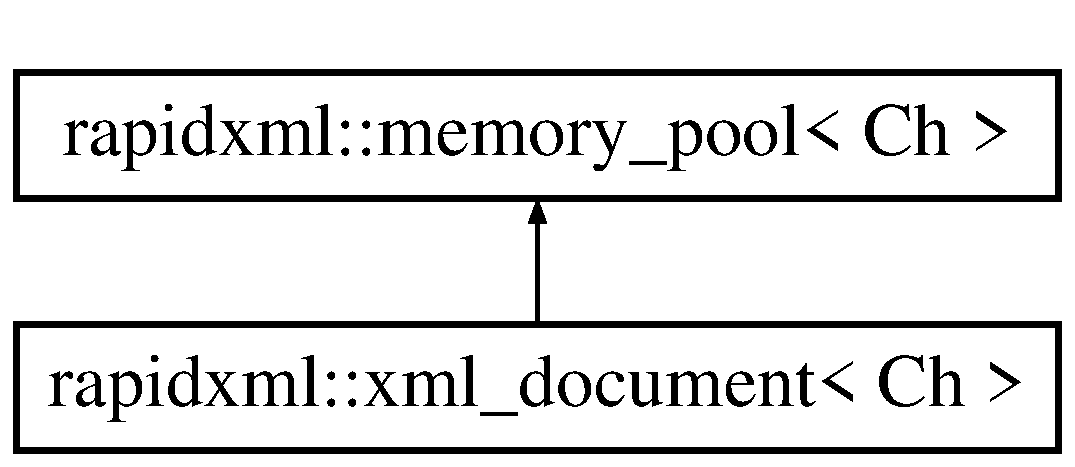
\includegraphics[height=2.000000cm]{classrapidxml_1_1memory__pool}
\end{center}
\end{figure}
\subsection*{Public Member Functions}
\begin{DoxyCompactItemize}
\item 
\mbox{\Hypertarget{classrapidxml_1_1memory__pool_a0b609da81dff28a19ebd704400788429}\label{classrapidxml_1_1memory__pool_a0b609da81dff28a19ebd704400788429}} 
\mbox{\hyperlink{classrapidxml_1_1memory__pool_a0b609da81dff28a19ebd704400788429}{memory\+\_\+pool}} ()
\begin{DoxyCompactList}\small\item\em Constructs empty pool with default allocator functions. \end{DoxyCompactList}\item 
\mbox{\hyperlink{classrapidxml_1_1memory__pool_a0a3e82126e59e4077f41e933130bb5a0}{$\sim$memory\+\_\+pool}} ()
\item 
\mbox{\hyperlink{classrapidxml_1_1xml__node}{xml\+\_\+node}}$<$ Ch $>$ $\ast$ \mbox{\hyperlink{classrapidxml_1_1memory__pool_a4118581c29ee9a2f6b55ebf7dac185f8}{allocate\+\_\+node}} (\mbox{\hyperlink{rapidxml_8hpp_abb456db38f7efb746c4330eed6072a7c}{node\+\_\+type}} type, const Ch $\ast$name=0, const Ch $\ast$value=0, std\+::size\+\_\+t name\+\_\+size=0, std\+::size\+\_\+t value\+\_\+size=0)
\item 
\mbox{\hyperlink{classrapidxml_1_1xml__attribute}{xml\+\_\+attribute}}$<$ Ch $>$ $\ast$ \mbox{\hyperlink{classrapidxml_1_1memory__pool_a3de2a66c983336e006ea3844e244ed30}{allocate\+\_\+attribute}} (const Ch $\ast$name=0, const Ch $\ast$value=0, std\+::size\+\_\+t name\+\_\+size=0, std\+::size\+\_\+t value\+\_\+size=0)
\item 
Ch $\ast$ \mbox{\hyperlink{classrapidxml_1_1memory__pool_a171941b39d55b868358da97462185f58}{allocate\+\_\+string}} (const Ch $\ast$source=0, std\+::size\+\_\+t size=0)
\item 
\mbox{\hyperlink{classrapidxml_1_1xml__node}{xml\+\_\+node}}$<$ Ch $>$ $\ast$ \mbox{\hyperlink{classrapidxml_1_1memory__pool_a0a10679fc17597d339a0dc107f8a94ac}{clone\+\_\+node}} (const \mbox{\hyperlink{classrapidxml_1_1xml__node}{xml\+\_\+node}}$<$ Ch $>$ $\ast$source, \mbox{\hyperlink{classrapidxml_1_1xml__node}{xml\+\_\+node}}$<$ Ch $>$ $\ast$result=0)
\item 
void \mbox{\hyperlink{classrapidxml_1_1memory__pool_aad377c835fdaed1cb2cc9df194cf84e4}{clear}} ()
\item 
void \mbox{\hyperlink{classrapidxml_1_1memory__pool_a84d3d8d2cdfc00501e1dcf26d889ae03}{set\+\_\+allocator}} (alloc\+\_\+func $\ast$af, free\+\_\+func $\ast$ff)
\end{DoxyCompactItemize}


\subsection{Detailed Description}
\subsubsection*{template$<$class Ch = char$>$\newline
class rapidxml\+::memory\+\_\+pool$<$ Ch $>$}

This class is used by the parser to create new nodes and attributes, without overheads of dynamic memory allocation. In most cases, you will not need to use this class directly. However, if you need to create nodes manually or modify names/values of nodes, you are encouraged to use \mbox{\hyperlink{classrapidxml_1_1memory__pool}{memory\+\_\+pool}} of relevant \mbox{\hyperlink{classrapidxml_1_1xml__document}{xml\+\_\+document}} to allocate the memory. Not only is this faster than allocating them by using {\ttfamily new} operator, but also their lifetime will be tied to the lifetime of document, possibly simplyfing memory management. ~\newline
~\newline
 Call \mbox{\hyperlink{classrapidxml_1_1memory__pool_a4118581c29ee9a2f6b55ebf7dac185f8}{allocate\+\_\+node()}} or \mbox{\hyperlink{classrapidxml_1_1memory__pool_a3de2a66c983336e006ea3844e244ed30}{allocate\+\_\+attribute()}} functions to obtain new nodes or attributes from the pool. You can also call \mbox{\hyperlink{classrapidxml_1_1memory__pool_a171941b39d55b868358da97462185f58}{allocate\+\_\+string()}} function to allocate strings. Such strings can then be used as names or values of nodes without worrying about their lifetime. Note that there is no {\ttfamily free()} function -- all allocations are freed at once when \mbox{\hyperlink{classrapidxml_1_1memory__pool_aad377c835fdaed1cb2cc9df194cf84e4}{clear()}} function is called, or when the pool is destroyed. ~\newline
~\newline
 It is also possible to create a standalone \mbox{\hyperlink{classrapidxml_1_1memory__pool}{memory\+\_\+pool}}, and use it to allocate nodes, whose lifetime will not be tied to any document. ~\newline
~\newline
 Pool maintains {\ttfamily R\+A\+P\+I\+D\+X\+M\+L\+\_\+\+S\+T\+A\+T\+I\+C\+\_\+\+P\+O\+O\+L\+\_\+\+S\+I\+ZE} bytes of statically allocated memory. Until static memory is exhausted, no dynamic memory allocations are done. When static memory is exhausted, pool allocates additional blocks of memory of size {\ttfamily R\+A\+P\+I\+D\+X\+M\+L\+\_\+\+D\+Y\+N\+A\+M\+I\+C\+\_\+\+P\+O\+O\+L\+\_\+\+S\+I\+ZE} each, by using global {\ttfamily new\mbox{[}\mbox{]}} and {\ttfamily delete\mbox{[}\mbox{]}} operators. This behaviour can be changed by setting custom allocation routines. Use \mbox{\hyperlink{classrapidxml_1_1memory__pool_a84d3d8d2cdfc00501e1dcf26d889ae03}{set\+\_\+allocator()}} function to set them. ~\newline
~\newline
 Allocations for nodes, attributes and strings are aligned at {\ttfamily R\+A\+P\+I\+D\+X\+M\+L\+\_\+\+A\+L\+I\+G\+N\+M\+E\+NT} bytes. This value defaults to the size of pointer on target architecture. ~\newline
~\newline
 To obtain absolutely top performance from the parser, it is important that all nodes are allocated from a single, contiguous block of memory. Otherwise, cache misses when jumping between two (or more) disjoint blocks of memory can slow down parsing quite considerably. If required, you can tweak {\ttfamily R\+A\+P\+I\+D\+X\+M\+L\+\_\+\+S\+T\+A\+T\+I\+C\+\_\+\+P\+O\+O\+L\+\_\+\+S\+I\+ZE}, {\ttfamily R\+A\+P\+I\+D\+X\+M\+L\+\_\+\+D\+Y\+N\+A\+M\+I\+C\+\_\+\+P\+O\+O\+L\+\_\+\+S\+I\+ZE} and {\ttfamily R\+A\+P\+I\+D\+X\+M\+L\+\_\+\+A\+L\+I\+G\+N\+M\+E\+NT} to obtain best wasted memory to performance compromise. To do it, define their values before \mbox{\hyperlink{rapidxml_8hpp}{rapidxml.\+hpp}} file is included. 
\begin{DoxyParams}{Parameters}
{\em Ch} & Character type of created nodes. \\
\hline
\end{DoxyParams}


\subsection{Constructor \& Destructor Documentation}
\mbox{\Hypertarget{classrapidxml_1_1memory__pool_a0a3e82126e59e4077f41e933130bb5a0}\label{classrapidxml_1_1memory__pool_a0a3e82126e59e4077f41e933130bb5a0}} 
\index{rapidxml\+::memory\+\_\+pool@{rapidxml\+::memory\+\_\+pool}!````~memory\+\_\+pool@{$\sim$memory\+\_\+pool}}
\index{````~memory\+\_\+pool@{$\sim$memory\+\_\+pool}!rapidxml\+::memory\+\_\+pool@{rapidxml\+::memory\+\_\+pool}}
\subsubsection{\texorpdfstring{$\sim$memory\+\_\+pool()}{~memory\_pool()}}
{\footnotesize\ttfamily template$<$class Ch  = char$>$ \\
\mbox{\hyperlink{classrapidxml_1_1memory__pool}{rapidxml\+::memory\+\_\+pool}}$<$ Ch $>$\+::$\sim$\mbox{\hyperlink{classrapidxml_1_1memory__pool}{memory\+\_\+pool}} (\begin{DoxyParamCaption}{ }\end{DoxyParamCaption})\hspace{0.3cm}{\ttfamily [inline]}}

Destroys pool and frees all the memory. This causes memory occupied by nodes allocated by the pool to be freed. Nodes allocated from the pool are no longer valid. 

\subsection{Member Function Documentation}
\mbox{\Hypertarget{classrapidxml_1_1memory__pool_a3de2a66c983336e006ea3844e244ed30}\label{classrapidxml_1_1memory__pool_a3de2a66c983336e006ea3844e244ed30}} 
\index{rapidxml\+::memory\+\_\+pool@{rapidxml\+::memory\+\_\+pool}!allocate\+\_\+attribute@{allocate\+\_\+attribute}}
\index{allocate\+\_\+attribute@{allocate\+\_\+attribute}!rapidxml\+::memory\+\_\+pool@{rapidxml\+::memory\+\_\+pool}}
\subsubsection{\texorpdfstring{allocate\+\_\+attribute()}{allocate\_attribute()}}
{\footnotesize\ttfamily template$<$class Ch  = char$>$ \\
\mbox{\hyperlink{classrapidxml_1_1xml__attribute}{xml\+\_\+attribute}}$<$Ch$>$$\ast$ \mbox{\hyperlink{classrapidxml_1_1memory__pool}{rapidxml\+::memory\+\_\+pool}}$<$ Ch $>$\+::allocate\+\_\+attribute (\begin{DoxyParamCaption}\item[{const Ch $\ast$}]{name = {\ttfamily 0},  }\item[{const Ch $\ast$}]{value = {\ttfamily 0},  }\item[{std\+::size\+\_\+t}]{name\+\_\+size = {\ttfamily 0},  }\item[{std\+::size\+\_\+t}]{value\+\_\+size = {\ttfamily 0} }\end{DoxyParamCaption})\hspace{0.3cm}{\ttfamily [inline]}}

Allocates a new attribute from the pool, and optionally assigns name and value to it. If the allocation request cannot be accomodated, this function will throw {\ttfamily std\+::bad\+\_\+alloc}. If exceptions are disabled by defining R\+A\+P\+I\+D\+X\+M\+L\+\_\+\+N\+O\+\_\+\+E\+X\+C\+E\+P\+T\+I\+O\+NS, this function will call rapidxml\+::parse\+\_\+error\+\_\+handler() function. 
\begin{DoxyParams}{Parameters}
{\em name} & Name to assign to the attribute, or 0 to assign no name. \\
\hline
{\em value} & Value to assign to the attribute, or 0 to assign no value. \\
\hline
{\em name\+\_\+size} & Size of name to assign, or 0 to automatically calculate size from name string. \\
\hline
{\em value\+\_\+size} & Size of value to assign, or 0 to automatically calculate size from value string. \\
\hline
\end{DoxyParams}
\begin{DoxyReturn}{Returns}
Pointer to allocated attribute. This pointer will never be N\+U\+LL. 
\end{DoxyReturn}
\mbox{\Hypertarget{classrapidxml_1_1memory__pool_a4118581c29ee9a2f6b55ebf7dac185f8}\label{classrapidxml_1_1memory__pool_a4118581c29ee9a2f6b55ebf7dac185f8}} 
\index{rapidxml\+::memory\+\_\+pool@{rapidxml\+::memory\+\_\+pool}!allocate\+\_\+node@{allocate\+\_\+node}}
\index{allocate\+\_\+node@{allocate\+\_\+node}!rapidxml\+::memory\+\_\+pool@{rapidxml\+::memory\+\_\+pool}}
\subsubsection{\texorpdfstring{allocate\+\_\+node()}{allocate\_node()}}
{\footnotesize\ttfamily template$<$class Ch  = char$>$ \\
\mbox{\hyperlink{classrapidxml_1_1xml__node}{xml\+\_\+node}}$<$Ch$>$$\ast$ \mbox{\hyperlink{classrapidxml_1_1memory__pool}{rapidxml\+::memory\+\_\+pool}}$<$ Ch $>$\+::allocate\+\_\+node (\begin{DoxyParamCaption}\item[{\mbox{\hyperlink{rapidxml_8hpp_abb456db38f7efb746c4330eed6072a7c}{node\+\_\+type}}}]{type,  }\item[{const Ch $\ast$}]{name = {\ttfamily 0},  }\item[{const Ch $\ast$}]{value = {\ttfamily 0},  }\item[{std\+::size\+\_\+t}]{name\+\_\+size = {\ttfamily 0},  }\item[{std\+::size\+\_\+t}]{value\+\_\+size = {\ttfamily 0} }\end{DoxyParamCaption})\hspace{0.3cm}{\ttfamily [inline]}}

Allocates a new node from the pool, and optionally assigns name and value to it. If the allocation request cannot be accomodated, this function will throw {\ttfamily std\+::bad\+\_\+alloc}. If exceptions are disabled by defining R\+A\+P\+I\+D\+X\+M\+L\+\_\+\+N\+O\+\_\+\+E\+X\+C\+E\+P\+T\+I\+O\+NS, this function will call rapidxml\+::parse\+\_\+error\+\_\+handler() function. 
\begin{DoxyParams}{Parameters}
{\em type} & Type of node to create. \\
\hline
{\em name} & Name to assign to the node, or 0 to assign no name. \\
\hline
{\em value} & Value to assign to the node, or 0 to assign no value. \\
\hline
{\em name\+\_\+size} & Size of name to assign, or 0 to automatically calculate size from name string. \\
\hline
{\em value\+\_\+size} & Size of value to assign, or 0 to automatically calculate size from value string. \\
\hline
\end{DoxyParams}
\begin{DoxyReturn}{Returns}
Pointer to allocated node. This pointer will never be N\+U\+LL. 
\end{DoxyReturn}
\mbox{\Hypertarget{classrapidxml_1_1memory__pool_a171941b39d55b868358da97462185f58}\label{classrapidxml_1_1memory__pool_a171941b39d55b868358da97462185f58}} 
\index{rapidxml\+::memory\+\_\+pool@{rapidxml\+::memory\+\_\+pool}!allocate\+\_\+string@{allocate\+\_\+string}}
\index{allocate\+\_\+string@{allocate\+\_\+string}!rapidxml\+::memory\+\_\+pool@{rapidxml\+::memory\+\_\+pool}}
\subsubsection{\texorpdfstring{allocate\+\_\+string()}{allocate\_string()}}
{\footnotesize\ttfamily template$<$class Ch  = char$>$ \\
Ch$\ast$ \mbox{\hyperlink{classrapidxml_1_1memory__pool}{rapidxml\+::memory\+\_\+pool}}$<$ Ch $>$\+::allocate\+\_\+string (\begin{DoxyParamCaption}\item[{const Ch $\ast$}]{source = {\ttfamily 0},  }\item[{std\+::size\+\_\+t}]{size = {\ttfamily 0} }\end{DoxyParamCaption})\hspace{0.3cm}{\ttfamily [inline]}}

Allocates a char array of given size from the pool, and optionally copies a given string to it. If the allocation request cannot be accomodated, this function will throw {\ttfamily std\+::bad\+\_\+alloc}. If exceptions are disabled by defining R\+A\+P\+I\+D\+X\+M\+L\+\_\+\+N\+O\+\_\+\+E\+X\+C\+E\+P\+T\+I\+O\+NS, this function will call rapidxml\+::parse\+\_\+error\+\_\+handler() function. 
\begin{DoxyParams}{Parameters}
{\em source} & String to initialize the allocated memory with, or 0 to not initialize it. \\
\hline
{\em size} & Number of characters to allocate, or zero to calculate it automatically from source string length; if size is 0, source string must be specified and null terminated. \\
\hline
\end{DoxyParams}
\begin{DoxyReturn}{Returns}
Pointer to allocated char array. This pointer will never be N\+U\+LL. 
\end{DoxyReturn}
\mbox{\Hypertarget{classrapidxml_1_1memory__pool_aad377c835fdaed1cb2cc9df194cf84e4}\label{classrapidxml_1_1memory__pool_aad377c835fdaed1cb2cc9df194cf84e4}} 
\index{rapidxml\+::memory\+\_\+pool@{rapidxml\+::memory\+\_\+pool}!clear@{clear}}
\index{clear@{clear}!rapidxml\+::memory\+\_\+pool@{rapidxml\+::memory\+\_\+pool}}
\subsubsection{\texorpdfstring{clear()}{clear()}}
{\footnotesize\ttfamily template$<$class Ch  = char$>$ \\
void \mbox{\hyperlink{classrapidxml_1_1memory__pool}{rapidxml\+::memory\+\_\+pool}}$<$ Ch $>$\+::clear (\begin{DoxyParamCaption}{ }\end{DoxyParamCaption})\hspace{0.3cm}{\ttfamily [inline]}}

Clears the pool. This causes memory occupied by nodes allocated by the pool to be freed. Any nodes or strings allocated from the pool will no longer be valid. \mbox{\Hypertarget{classrapidxml_1_1memory__pool_a0a10679fc17597d339a0dc107f8a94ac}\label{classrapidxml_1_1memory__pool_a0a10679fc17597d339a0dc107f8a94ac}} 
\index{rapidxml\+::memory\+\_\+pool@{rapidxml\+::memory\+\_\+pool}!clone\+\_\+node@{clone\+\_\+node}}
\index{clone\+\_\+node@{clone\+\_\+node}!rapidxml\+::memory\+\_\+pool@{rapidxml\+::memory\+\_\+pool}}
\subsubsection{\texorpdfstring{clone\+\_\+node()}{clone\_node()}}
{\footnotesize\ttfamily template$<$class Ch  = char$>$ \\
\mbox{\hyperlink{classrapidxml_1_1xml__node}{xml\+\_\+node}}$<$Ch$>$$\ast$ \mbox{\hyperlink{classrapidxml_1_1memory__pool}{rapidxml\+::memory\+\_\+pool}}$<$ Ch $>$\+::clone\+\_\+node (\begin{DoxyParamCaption}\item[{const \mbox{\hyperlink{classrapidxml_1_1xml__node}{xml\+\_\+node}}$<$ Ch $>$ $\ast$}]{source,  }\item[{\mbox{\hyperlink{classrapidxml_1_1xml__node}{xml\+\_\+node}}$<$ Ch $>$ $\ast$}]{result = {\ttfamily 0} }\end{DoxyParamCaption})\hspace{0.3cm}{\ttfamily [inline]}}

Clones an \mbox{\hyperlink{classrapidxml_1_1xml__node}{xml\+\_\+node}} and its hierarchy of child nodes and attributes. Nodes and attributes are allocated from this memory pool. Names and values are not cloned, they are shared between the clone and the source. Result node can be optionally specified as a second parameter, in which case its contents will be replaced with cloned source node. This is useful when you want to clone entire document. 
\begin{DoxyParams}{Parameters}
{\em source} & Node to clone. \\
\hline
{\em result} & Node to put results in, or 0 to automatically allocate result node \\
\hline
\end{DoxyParams}
\begin{DoxyReturn}{Returns}
Pointer to cloned node. This pointer will never be N\+U\+LL. 
\end{DoxyReturn}
\mbox{\Hypertarget{classrapidxml_1_1memory__pool_a84d3d8d2cdfc00501e1dcf26d889ae03}\label{classrapidxml_1_1memory__pool_a84d3d8d2cdfc00501e1dcf26d889ae03}} 
\index{rapidxml\+::memory\+\_\+pool@{rapidxml\+::memory\+\_\+pool}!set\+\_\+allocator@{set\+\_\+allocator}}
\index{set\+\_\+allocator@{set\+\_\+allocator}!rapidxml\+::memory\+\_\+pool@{rapidxml\+::memory\+\_\+pool}}
\subsubsection{\texorpdfstring{set\+\_\+allocator()}{set\_allocator()}}
{\footnotesize\ttfamily template$<$class Ch  = char$>$ \\
void \mbox{\hyperlink{classrapidxml_1_1memory__pool}{rapidxml\+::memory\+\_\+pool}}$<$ Ch $>$\+::set\+\_\+allocator (\begin{DoxyParamCaption}\item[{alloc\+\_\+func $\ast$}]{af,  }\item[{free\+\_\+func $\ast$}]{ff }\end{DoxyParamCaption})\hspace{0.3cm}{\ttfamily [inline]}}

Sets or resets the user-\/defined memory allocation functions for the pool. This can only be called when no memory is allocated from the pool yet, otherwise results are undefined. Allocation function must not return invalid pointer on failure. It should either throw, stop the program, or use {\ttfamily longjmp()} function to pass control to other place of program. If it returns invalid pointer, results are undefined. ~\newline
~\newline
 User defined allocation functions must have the following forms\+: ~\newline
{\ttfamily  ~\newline
void $\ast$allocate(std\+::size\+\_\+t size); ~\newline
void free(void $\ast$pointer); }~\newline
 
\begin{DoxyParams}{Parameters}
{\em af} & Allocation function, or 0 to restore default function \\
\hline
{\em ff} & Free function, or 0 to restore default function \\
\hline
\end{DoxyParams}


The documentation for this class was generated from the following file\+:\begin{DoxyCompactItemize}
\item 
\mbox{\hyperlink{rapidxml_8hpp}{rapidxml.\+hpp}}\end{DoxyCompactItemize}

\hypertarget{classtfp_1_1_mouse}{}\section{tfp\+:\+:Mouse Class Reference}
\label{classtfp_1_1_mouse}\index{tfp\+::\+Mouse@{tfp\+::\+Mouse}}
\subsection*{Public Member Functions}
\begin{DoxyCompactItemize}
\item 
\mbox{\Hypertarget{classtfp_1_1_mouse_a0544d0e8c26cdd2f4d7ce7a73ae10529}\label{classtfp_1_1_mouse_a0544d0e8c26cdd2f4d7ce7a73ae10529}} 
\mbox{\hyperlink{classtfp_1_1_mouse_a0544d0e8c26cdd2f4d7ce7a73ae10529}{Mouse}} ()
\begin{DoxyCompactList}\small\item\em Konstruktor. \end{DoxyCompactList}\item 
\mbox{\Hypertarget{classtfp_1_1_mouse_afb2244bb9f0e2ebfc55a13b30c498c60}\label{classtfp_1_1_mouse_afb2244bb9f0e2ebfc55a13b30c498c60}} 
\mbox{\hyperlink{classtfp_1_1_mouse_afb2244bb9f0e2ebfc55a13b30c498c60}{$\sim$\+Mouse}} ()
\begin{DoxyCompactList}\small\item\em Destruktor. \end{DoxyCompactList}\item 
\mbox{\Hypertarget{classtfp_1_1_mouse_a026645fcd024169978c3e3567a681dfa}\label{classtfp_1_1_mouse_a026645fcd024169978c3e3567a681dfa}} 
const sf\+::\+Vector2f \& \mbox{\hyperlink{classtfp_1_1_mouse_a026645fcd024169978c3e3567a681dfa}{Get\+Mouse\+Position}} ()
\begin{DoxyCompactList}\small\item\em Zwraca pozycje myszy w oknie. \end{DoxyCompactList}\item 
\mbox{\Hypertarget{classtfp_1_1_mouse_ac76c2bb7580ac4c678640d3a0e27a17a}\label{classtfp_1_1_mouse_ac76c2bb7580ac4c678640d3a0e27a17a}} 
const sf\+::\+Vector2f \mbox{\hyperlink{classtfp_1_1_mouse_ac76c2bb7580ac4c678640d3a0e27a17a}{Get\+Mouse\+Position\+Scaled}} ()
\begin{DoxyCompactList}\small\item\em Zwraca przeskalowana pozycje myszy w oknie. \end{DoxyCompactList}\item 
\mbox{\Hypertarget{classtfp_1_1_mouse_a1f055556ba7923eae41e8bb0c309ebc5}\label{classtfp_1_1_mouse_a1f055556ba7923eae41e8bb0c309ebc5}} 
const sf\+::\+Vector2f \mbox{\hyperlink{classtfp_1_1_mouse_a1f055556ba7923eae41e8bb0c309ebc5}{Get\+Mouse\+Position\+On\+Map}} ()
\begin{DoxyCompactList}\small\item\em Zwraca pozycje myszy na mapie. \end{DoxyCompactList}\item 
\mbox{\Hypertarget{classtfp_1_1_mouse_a4e94ce206c7ee9476c58474d870b19ed}\label{classtfp_1_1_mouse_a4e94ce206c7ee9476c58474d870b19ed}} 
sf\+::\+Mouse \& \mbox{\hyperlink{classtfp_1_1_mouse_a4e94ce206c7ee9476c58474d870b19ed}{Get\+Mouse}} ()
\begin{DoxyCompactList}\small\item\em Zwraca bezposredni obiekt sf\+::\+Mouse. \end{DoxyCompactList}\item 
\mbox{\Hypertarget{classtfp_1_1_mouse_af75de19ef50018ac5e1034957e115d05}\label{classtfp_1_1_mouse_af75de19ef50018ac5e1034957e115d05}} 
void \mbox{\hyperlink{classtfp_1_1_mouse_af75de19ef50018ac5e1034957e115d05}{Set\+Game\+Handle}} (\mbox{\hyperlink{classtfp_1_1_game}{tfp\+::\+Game}} $\ast$Handle)
\begin{DoxyCompactList}\small\item\em Ustawia uchwyt gry. \end{DoxyCompactList}\item 
void \mbox{\hyperlink{classtfp_1_1_mouse_a9cad9f88ae445c0bca5eb489216e4160}{Load\+Data}} ()
\begin{DoxyCompactList}\small\item\em Pobiera informacje o myszce. \end{DoxyCompactList}\item 
\mbox{\Hypertarget{classtfp_1_1_mouse_a522779ab55451c915ae4451561062c95}\label{classtfp_1_1_mouse_a522779ab55451c915ae4451561062c95}} 
const sf\+::\+Vector2f \mbox{\hyperlink{classtfp_1_1_mouse_a522779ab55451c915ae4451561062c95}{Get\+Left\+Mouse\+Button\+Delta\+Drag}} () const
\begin{DoxyCompactList}\small\item\em Zwraca przeciagniecie lewym przyciskiem myszy. \end{DoxyCompactList}\item 
\mbox{\Hypertarget{classtfp_1_1_mouse_a48a1f58c7e4786b1be82cecef9fa6a41}\label{classtfp_1_1_mouse_a48a1f58c7e4786b1be82cecef9fa6a41}} 
const sf\+::\+Vector2f \mbox{\hyperlink{classtfp_1_1_mouse_a48a1f58c7e4786b1be82cecef9fa6a41}{Get\+Right\+Mouse\+Button\+Delta\+Drag}} () const
\begin{DoxyCompactList}\small\item\em Zwraca przeciagniecie prawym przyciskiem myszy. \end{DoxyCompactList}\item 
\mbox{\Hypertarget{classtfp_1_1_mouse_af8fabd17deb9f825666262e754e8b9b8}\label{classtfp_1_1_mouse_af8fabd17deb9f825666262e754e8b9b8}} 
const sf\+::\+Vector2f \mbox{\hyperlink{classtfp_1_1_mouse_af8fabd17deb9f825666262e754e8b9b8}{Get\+Left\+Mouse\+Button\+Delta\+Drag\+Scaled}} ()
\begin{DoxyCompactList}\small\item\em Zwraca przeskalowane przeciagniecie lewym przyciskiem myszy. \end{DoxyCompactList}\item 
\mbox{\Hypertarget{classtfp_1_1_mouse_a3039a60ae3314a4bf27ebb77b5a70661}\label{classtfp_1_1_mouse_a3039a60ae3314a4bf27ebb77b5a70661}} 
const sf\+::\+Vector2f \mbox{\hyperlink{classtfp_1_1_mouse_a3039a60ae3314a4bf27ebb77b5a70661}{Get\+Right\+Mouse\+Button\+Delta\+Drag\+Scaled}} ()
\begin{DoxyCompactList}\small\item\em Zwraca przeskalowane przeciagniecie prawym przyciskiem myszy. \end{DoxyCompactList}\end{DoxyCompactItemize}


\subsection{Member Function Documentation}
\mbox{\Hypertarget{classtfp_1_1_mouse_a9cad9f88ae445c0bca5eb489216e4160}\label{classtfp_1_1_mouse_a9cad9f88ae445c0bca5eb489216e4160}} 
\index{tfp\+::\+Mouse@{tfp\+::\+Mouse}!Load\+Data@{Load\+Data}}
\index{Load\+Data@{Load\+Data}!tfp\+::\+Mouse@{tfp\+::\+Mouse}}
\subsubsection{\texorpdfstring{Load\+Data()}{LoadData()}}
{\footnotesize\ttfamily void tfp\+::\+Mouse\+::\+Load\+Data (\begin{DoxyParamCaption}{ }\end{DoxyParamCaption})}



Pobiera informacje o myszce. 

L\+PM

P\+PM 

The documentation for this class was generated from the following files\+:\begin{DoxyCompactItemize}
\item 
mouse.\+hpp\item 
mouse.\+cpp\end{DoxyCompactItemize}

\hypertarget{classtfp_1_1_network_client}{}\section{tfp\+:\+:Network\+Client Class Reference}
\label{classtfp_1_1_network_client}\index{tfp\+::\+Network\+Client@{tfp\+::\+Network\+Client}}
\subsection*{Public Member Functions}
\begin{DoxyCompactItemize}
\item 
\mbox{\Hypertarget{classtfp_1_1_network_client_a1b07ca395f5735504a988455729ae364}\label{classtfp_1_1_network_client_a1b07ca395f5735504a988455729ae364}} 
\mbox{\hyperlink{classtfp_1_1_network_client_a1b07ca395f5735504a988455729ae364}{Network\+Client}} ()
\begin{DoxyCompactList}\small\item\em Constructor. \end{DoxyCompactList}\item 
\mbox{\Hypertarget{classtfp_1_1_network_client_aa1e3a0394998e327f67b7d41a63fcf18}\label{classtfp_1_1_network_client_aa1e3a0394998e327f67b7d41a63fcf18}} 
\mbox{\hyperlink{classtfp_1_1_network_client_aa1e3a0394998e327f67b7d41a63fcf18}{$\sim$\+Network\+Client}} ()
\begin{DoxyCompactList}\small\item\em Destructor. \end{DoxyCompactList}\item 
\mbox{\Hypertarget{classtfp_1_1_network_client_a894a282f89df561709478c68a30bfd41}\label{classtfp_1_1_network_client_a894a282f89df561709478c68a30bfd41}} 
void \mbox{\hyperlink{classtfp_1_1_network_client_a894a282f89df561709478c68a30bfd41}{Set\+Game\+Handle}} (\mbox{\hyperlink{classtfp_1_1_game}{tfp\+::\+Game}} $\ast$Game\+Handle)
\begin{DoxyCompactList}\small\item\em Set game handle. \end{DoxyCompactList}\item 
\mbox{\Hypertarget{classtfp_1_1_network_client_a6baa9740eb622e2fde85a07ea4dd9614}\label{classtfp_1_1_network_client_a6baa9740eb622e2fde85a07ea4dd9614}} 
void \mbox{\hyperlink{classtfp_1_1_network_client_a6baa9740eb622e2fde85a07ea4dd9614}{Run}} (std\+::string Server\+Ip, int Server\+Port)
\begin{DoxyCompactList}\small\item\em Starts client in a new thread. \end{DoxyCompactList}\item 
\mbox{\Hypertarget{classtfp_1_1_network_client_a8753f0074647aa3596aece10ebb90796}\label{classtfp_1_1_network_client_a8753f0074647aa3596aece10ebb90796}} 
void \mbox{\hyperlink{classtfp_1_1_network_client_a8753f0074647aa3596aece10ebb90796}{Stop}} ()
\begin{DoxyCompactList}\small\item\em Stops client thread. \end{DoxyCompactList}\item 
\mbox{\Hypertarget{classtfp_1_1_network_client_ac161ba71ecfdc85a870b5d49e6e5e1a5}\label{classtfp_1_1_network_client_ac161ba71ecfdc85a870b5d49e6e5e1a5}} 
void \mbox{\hyperlink{classtfp_1_1_network_client_ac161ba71ecfdc85a870b5d49e6e5e1a5}{Send\+Command\+To\+Server}} (std\+::string Command)
\begin{DoxyCompactList}\small\item\em Sends command to a server. \end{DoxyCompactList}\item 
\mbox{\Hypertarget{classtfp_1_1_network_client_aff643ad46db23b639bd177832848f1a0}\label{classtfp_1_1_network_client_aff643ad46db23b639bd177832848f1a0}} 
void \mbox{\hyperlink{classtfp_1_1_network_client_aff643ad46db23b639bd177832848f1a0}{Set\+Client\+Id}} (int Client\+Id)
\begin{DoxyCompactList}\small\item\em Sets client ID. \end{DoxyCompactList}\item 
\mbox{\Hypertarget{classtfp_1_1_network_client_a715cef2522038f12b712e5c5ea93d5c0}\label{classtfp_1_1_network_client_a715cef2522038f12b712e5c5ea93d5c0}} 
bool \mbox{\hyperlink{classtfp_1_1_network_client_a715cef2522038f12b712e5c5ea93d5c0}{Is\+Connected}} ()
\begin{DoxyCompactList}\small\item\em Return if client is connected to a server. \end{DoxyCompactList}\end{DoxyCompactItemize}


The documentation for this class was generated from the following files\+:\begin{DoxyCompactItemize}
\item 
client.\+hpp\item 
client.\+cpp\end{DoxyCompactItemize}

\hypertarget{classtfp_1_1_network_server}{}\section{tfp\+:\+:Network\+Server Class Reference}
\label{classtfp_1_1_network_server}\index{tfp\+::\+Network\+Server@{tfp\+::\+Network\+Server}}
\subsection*{Public Member Functions}
\begin{DoxyCompactItemize}
\item 
\mbox{\Hypertarget{classtfp_1_1_network_server_a02057a60aa95fae70c8379faa03c79fc}\label{classtfp_1_1_network_server_a02057a60aa95fae70c8379faa03c79fc}} 
\mbox{\hyperlink{classtfp_1_1_network_server_a02057a60aa95fae70c8379faa03c79fc}{Network\+Server}} ()
\begin{DoxyCompactList}\small\item\em Constructor. \end{DoxyCompactList}\item 
\mbox{\Hypertarget{classtfp_1_1_network_server_ac2fed7f35725052c48ec0c7bd9e1f2d9}\label{classtfp_1_1_network_server_ac2fed7f35725052c48ec0c7bd9e1f2d9}} 
\mbox{\hyperlink{classtfp_1_1_network_server_ac2fed7f35725052c48ec0c7bd9e1f2d9}{$\sim$\+Network\+Server}} ()
\begin{DoxyCompactList}\small\item\em Destructor. \end{DoxyCompactList}\item 
\mbox{\Hypertarget{classtfp_1_1_network_server_affeadcb842da50c78f47b46e3663eff3}\label{classtfp_1_1_network_server_affeadcb842da50c78f47b46e3663eff3}} 
void \mbox{\hyperlink{classtfp_1_1_network_server_affeadcb842da50c78f47b46e3663eff3}{Set\+Game\+Handle}} (\mbox{\hyperlink{classtfp_1_1_game}{tfp\+::\+Game}} $\ast$Game\+Handle)
\begin{DoxyCompactList}\small\item\em Set game handle. \end{DoxyCompactList}\item 
\mbox{\Hypertarget{classtfp_1_1_network_server_a7cb2e252d7443e31f5ddd0bdec29f7e5}\label{classtfp_1_1_network_server_a7cb2e252d7443e31f5ddd0bdec29f7e5}} 
void \mbox{\hyperlink{classtfp_1_1_network_server_a7cb2e252d7443e31f5ddd0bdec29f7e5}{Run}} (sf\+::\+Ip\+Address Server\+Ip, int Server\+Port)
\begin{DoxyCompactList}\small\item\em Starts server in a new thread. \end{DoxyCompactList}\item 
\mbox{\Hypertarget{classtfp_1_1_network_server_ae471e474cb57201defdafa99e4a5a538}\label{classtfp_1_1_network_server_ae471e474cb57201defdafa99e4a5a538}} 
void \mbox{\hyperlink{classtfp_1_1_network_server_ae471e474cb57201defdafa99e4a5a538}{Stop}} ()
\begin{DoxyCompactList}\small\item\em Stops server thread. \end{DoxyCompactList}\item 
\mbox{\Hypertarget{classtfp_1_1_network_server_aa102c86afba78c1b27d3c68af7dd6d16}\label{classtfp_1_1_network_server_aa102c86afba78c1b27d3c68af7dd6d16}} 
void \mbox{\hyperlink{classtfp_1_1_network_server_aa102c86afba78c1b27d3c68af7dd6d16}{Send\+Command\+To\+Clients}} (std\+::string Command, int Id=-\/1)
\begin{DoxyCompactList}\small\item\em Sends command to a server. \end{DoxyCompactList}\end{DoxyCompactItemize}


The documentation for this class was generated from the following files\+:\begin{DoxyCompactItemize}
\item 
server.\+hpp\item 
server.\+cpp\end{DoxyCompactItemize}

\hypertarget{classtfp_1_1specialeffects_1_1_night}{}\section{tfp\+:\+:specialeffects\+:\+:Night Class Reference}
\label{classtfp_1_1specialeffects_1_1_night}\index{tfp\+::specialeffects\+::\+Night@{tfp\+::specialeffects\+::\+Night}}
\subsection*{Public Member Functions}
\begin{DoxyCompactItemize}
\item 
\mbox{\Hypertarget{classtfp_1_1specialeffects_1_1_night_a6e8fece76928d856e589996881bfbb90}\label{classtfp_1_1specialeffects_1_1_night_a6e8fece76928d856e589996881bfbb90}} 
\mbox{\hyperlink{classtfp_1_1specialeffects_1_1_night_a6e8fece76928d856e589996881bfbb90}{Night}} ()
\begin{DoxyCompactList}\small\item\em Constructor. \end{DoxyCompactList}\item 
\mbox{\Hypertarget{classtfp_1_1specialeffects_1_1_night_a24aab4e13a82752b128ec6c0a5402efa}\label{classtfp_1_1specialeffects_1_1_night_a24aab4e13a82752b128ec6c0a5402efa}} 
\mbox{\hyperlink{classtfp_1_1specialeffects_1_1_night_a24aab4e13a82752b128ec6c0a5402efa}{$\sim$\+Night}} ()
\begin{DoxyCompactList}\small\item\em Destructor. \end{DoxyCompactList}\item 
void \mbox{\hyperlink{classtfp_1_1specialeffects_1_1_night_acf90989e3e036bd3c45a8096809a31a5}{Set\+Game\+Handle}} (\mbox{\hyperlink{classtfp_1_1_game}{tfp\+::\+Game}} $\ast$Handle)
\begin{DoxyCompactList}\small\item\em Sets game handle. \end{DoxyCompactList}\item 
\mbox{\Hypertarget{classtfp_1_1specialeffects_1_1_night_a015dba4b8752225e95d3f9d683a12391}\label{classtfp_1_1specialeffects_1_1_night_a015dba4b8752225e95d3f9d683a12391}} 
void \mbox{\hyperlink{classtfp_1_1specialeffects_1_1_night_a015dba4b8752225e95d3f9d683a12391}{Display}} ()
\begin{DoxyCompactList}\small\item\em Render night effect. \end{DoxyCompactList}\item 
\mbox{\Hypertarget{classtfp_1_1specialeffects_1_1_night_ae6bc6a73197bea6bf34ecf80145194f5}\label{classtfp_1_1specialeffects_1_1_night_ae6bc6a73197bea6bf34ecf80145194f5}} 
void \mbox{\hyperlink{classtfp_1_1specialeffects_1_1_night_ae6bc6a73197bea6bf34ecf80145194f5}{Set\+Darkness}} (int Value)
\begin{DoxyCompactList}\small\item\em Sets how dark is night. \end{DoxyCompactList}\item 
\mbox{\Hypertarget{classtfp_1_1specialeffects_1_1_night_a50cfa54522d03b0e2dc2fb111ac2dfd2}\label{classtfp_1_1specialeffects_1_1_night_a50cfa54522d03b0e2dc2fb111ac2dfd2}} 
void \mbox{\hyperlink{classtfp_1_1specialeffects_1_1_night_a50cfa54522d03b0e2dc2fb111ac2dfd2}{Set\+Darkness\+Opacity}} (int Value)
\begin{DoxyCompactList}\small\item\em Sets temporary darkness that is rendered if lightning is enabled. \end{DoxyCompactList}\item 
\mbox{\Hypertarget{classtfp_1_1specialeffects_1_1_night_a7926d8c9965454d69ce1d235a9fca941}\label{classtfp_1_1specialeffects_1_1_night_a7926d8c9965454d69ce1d235a9fca941}} 
void \mbox{\hyperlink{classtfp_1_1specialeffects_1_1_night_a7926d8c9965454d69ce1d235a9fca941}{Set\+Lighter}} (bool State)
\begin{DoxyCompactList}\small\item\em Turns on/off lighter (area on the middle that is not affected by night) \end{DoxyCompactList}\item 
\mbox{\Hypertarget{classtfp_1_1specialeffects_1_1_night_ad26fc86c16eba1803624be2c52dce3d5}\label{classtfp_1_1specialeffects_1_1_night_ad26fc86c16eba1803624be2c52dce3d5}} 
bool \mbox{\hyperlink{classtfp_1_1specialeffects_1_1_night_ad26fc86c16eba1803624be2c52dce3d5}{Is\+Lighter\+On}} ()
\begin{DoxyCompactList}\small\item\em Returns if lighter is on. \end{DoxyCompactList}\end{DoxyCompactItemize}


\subsection{Member Function Documentation}
\mbox{\Hypertarget{classtfp_1_1specialeffects_1_1_night_acf90989e3e036bd3c45a8096809a31a5}\label{classtfp_1_1specialeffects_1_1_night_acf90989e3e036bd3c45a8096809a31a5}} 
\index{tfp\+::specialeffects\+::\+Night@{tfp\+::specialeffects\+::\+Night}!Set\+Game\+Handle@{Set\+Game\+Handle}}
\index{Set\+Game\+Handle@{Set\+Game\+Handle}!tfp\+::specialeffects\+::\+Night@{tfp\+::specialeffects\+::\+Night}}
\subsubsection{\texorpdfstring{Set\+Game\+Handle()}{SetGameHandle()}}
{\footnotesize\ttfamily void tfp\+::specialeffects\+::\+Night\+::\+Set\+Game\+Handle (\begin{DoxyParamCaption}\item[{\mbox{\hyperlink{classtfp_1_1_game}{tfp\+::\+Game}} $\ast$}]{Handle }\end{DoxyParamCaption})}



Sets game handle. 

\mbox{\hyperlink{classtfp_1_1specialeffects_1_1_night}{Night}}. 

The documentation for this class was generated from the following files\+:\begin{DoxyCompactItemize}
\item 
interfaceffects.\+hpp\item 
interfaceffects.\+cpp\end{DoxyCompactItemize}

\hypertarget{structtfp_1_1_key_config_class_1_1_node}{}\section{tfp\+:\+:Key\+Config\+Class\+:\+:Node Struct Reference}
\label{structtfp_1_1_key_config_class_1_1_node}\index{tfp\+::\+Key\+Config\+Class\+::\+Node@{tfp\+::\+Key\+Config\+Class\+::\+Node}}
\subsection*{Public Attributes}
\begin{DoxyCompactItemize}
\item 
\mbox{\Hypertarget{structtfp_1_1_key_config_class_1_1_node_a89020ad9ac07b45e05881f1ad9a3f201}\label{structtfp_1_1_key_config_class_1_1_node_a89020ad9ac07b45e05881f1ad9a3f201}} 
int {\bfseries Key\+Code}
\item 
\mbox{\Hypertarget{structtfp_1_1_key_config_class_1_1_node_a406df5e518bf88d13eedb59649ec0033}\label{structtfp_1_1_key_config_class_1_1_node_a406df5e518bf88d13eedb59649ec0033}} 
bool {\bfseries Key\+System}
\item 
\mbox{\Hypertarget{structtfp_1_1_key_config_class_1_1_node_ab308cf66de9abc55470f3251536d168d}\label{structtfp_1_1_key_config_class_1_1_node_ab308cf66de9abc55470f3251536d168d}} 
bool {\bfseries Key\+Alt}
\item 
\mbox{\Hypertarget{structtfp_1_1_key_config_class_1_1_node_aad0c0984be5056abdb858117f105f2c2}\label{structtfp_1_1_key_config_class_1_1_node_aad0c0984be5056abdb858117f105f2c2}} 
bool {\bfseries Key\+Shift}
\item 
\mbox{\Hypertarget{structtfp_1_1_key_config_class_1_1_node_a67945af4ed76fb1869626dce57aff18e}\label{structtfp_1_1_key_config_class_1_1_node_a67945af4ed76fb1869626dce57aff18e}} 
bool {\bfseries Key\+Control}
\item 
\mbox{\Hypertarget{structtfp_1_1_key_config_class_1_1_node_ae88d85e7a8d86148bd9454131219768a}\label{structtfp_1_1_key_config_class_1_1_node_ae88d85e7a8d86148bd9454131219768a}} 
std\+::string {\bfseries Action\+Name}
\end{DoxyCompactItemize}


The documentation for this struct was generated from the following file\+:\begin{DoxyCompactItemize}
\item 
keyconfiguration.\+hpp\end{DoxyCompactItemize}

\hypertarget{structtfp_1_1_area_list_class_1_1_node}{}\section{tfp\+:\+:Area\+List\+Class\+:\+:Node Struct Reference}
\label{structtfp_1_1_area_list_class_1_1_node}\index{tfp\+::\+Area\+List\+Class\+::\+Node@{tfp\+::\+Area\+List\+Class\+::\+Node}}
\subsection*{Public Types}
\begin{DoxyCompactItemize}
\item 
\mbox{\Hypertarget{structtfp_1_1_area_list_class_1_1_node_aed23600f7feae23c7ad61ecf8247e871}\label{structtfp_1_1_area_list_class_1_1_node_aed23600f7feae23c7ad61ecf8247e871}} 
enum {\bfseries Area\+Type} \{ {\bfseries Focus}, 
{\bfseries Dragable}, 
{\bfseries Clickable}, 
{\bfseries Input}
 \}
\end{DoxyCompactItemize}
\subsection*{Public Member Functions}
\begin{DoxyCompactItemize}
\item 
\mbox{\Hypertarget{structtfp_1_1_area_list_class_1_1_node_a72a51811ed96156e9bfa66fe4c14a2fd}\label{structtfp_1_1_area_list_class_1_1_node_a72a51811ed96156e9bfa66fe4c14a2fd}} 
{\bfseries Node} (\mbox{\hyperlink{classtfp_1_1_focus_area}{tfp\+::\+Focus\+Area}} $\ast$Handle)
\item 
\mbox{\Hypertarget{structtfp_1_1_area_list_class_1_1_node_a41c088c2942d5db89b3be0bc7fefabf5}\label{structtfp_1_1_area_list_class_1_1_node_a41c088c2942d5db89b3be0bc7fefabf5}} 
{\bfseries Node} (\mbox{\hyperlink{classtfp_1_1_dragable_area}{tfp\+::\+Dragable\+Area}} $\ast$Handle)
\item 
\mbox{\Hypertarget{structtfp_1_1_area_list_class_1_1_node_ab60f41b782685daf89db46cddbe7e25c}\label{structtfp_1_1_area_list_class_1_1_node_ab60f41b782685daf89db46cddbe7e25c}} 
{\bfseries Node} (\mbox{\hyperlink{classtfp_1_1_clickable_area}{tfp\+::\+Clickable\+Area}} $\ast$Handle)
\item 
\mbox{\Hypertarget{structtfp_1_1_area_list_class_1_1_node_a2756be2f207b4f37ed8d8cf2f1b4902e}\label{structtfp_1_1_area_list_class_1_1_node_a2756be2f207b4f37ed8d8cf2f1b4902e}} 
{\bfseries Node} (\mbox{\hyperlink{classtfp_1_1_input_area}{tfp\+::\+Input\+Area}} $\ast$Handle)
\end{DoxyCompactItemize}
\subsection*{Public Attributes}
\begin{DoxyCompactItemize}
\item 
\mbox{\Hypertarget{structtfp_1_1_area_list_class_1_1_node_a02061da52a83b6b6670a52828acb4070}\label{structtfp_1_1_area_list_class_1_1_node_a02061da52a83b6b6670a52828acb4070}} 
\mbox{\hyperlink{classtfp_1_1_focus_area}{tfp\+::\+Focus\+Area}} $\ast$ {\bfseries Focus\+Area\+Handle}
\item 
\mbox{\Hypertarget{structtfp_1_1_area_list_class_1_1_node_ab46a54b11ca6e1e4bcdeb678d2de2d25}\label{structtfp_1_1_area_list_class_1_1_node_ab46a54b11ca6e1e4bcdeb678d2de2d25}} 
\mbox{\hyperlink{classtfp_1_1_dragable_area}{tfp\+::\+Dragable\+Area}} $\ast$ {\bfseries Dragable\+Area\+Handle}
\item 
\mbox{\Hypertarget{structtfp_1_1_area_list_class_1_1_node_a8d5ad2e1b4303fa7504574867a0d6484}\label{structtfp_1_1_area_list_class_1_1_node_a8d5ad2e1b4303fa7504574867a0d6484}} 
\mbox{\hyperlink{classtfp_1_1_clickable_area}{tfp\+::\+Clickable\+Area}} $\ast$ {\bfseries Clickable\+Area\+Handle}
\item 
\mbox{\Hypertarget{structtfp_1_1_area_list_class_1_1_node_aabd321fde79cea8d6a331b616a02634b}\label{structtfp_1_1_area_list_class_1_1_node_aabd321fde79cea8d6a331b616a02634b}} 
\mbox{\hyperlink{classtfp_1_1_input_area}{tfp\+::\+Input\+Area}} $\ast$ {\bfseries Input\+Area\+Handle}
\item 
\mbox{\Hypertarget{structtfp_1_1_area_list_class_1_1_node_adc6c2b6feb7797349a9823649ce8dba6}\label{structtfp_1_1_area_list_class_1_1_node_adc6c2b6feb7797349a9823649ce8dba6}} 
Area\+Type {\bfseries Type}
\end{DoxyCompactItemize}


The documentation for this struct was generated from the following files\+:\begin{DoxyCompactItemize}
\item 
area.\+hpp\item 
area.\+cpp\end{DoxyCompactItemize}

\hypertarget{classrapidxml_1_1node__iterator}{}\section{rapidxml\+:\+:node\+\_\+iterator$<$ Ch $>$ Class Template Reference}
\label{classrapidxml_1_1node__iterator}\index{rapidxml\+::node\+\_\+iterator$<$ Ch $>$@{rapidxml\+::node\+\_\+iterator$<$ Ch $>$}}


Iterator of child nodes of \mbox{\hyperlink{classrapidxml_1_1xml__node}{xml\+\_\+node}}.  




{\ttfamily \#include $<$rapidxml\+\_\+iterators.\+hpp$>$}

\subsection*{Public Types}
\begin{DoxyCompactItemize}
\item 
\mbox{\Hypertarget{classrapidxml_1_1node__iterator_ade6310119ed1f72c94830e006fac69b7}\label{classrapidxml_1_1node__iterator_ade6310119ed1f72c94830e006fac69b7}} 
typedef \mbox{\hyperlink{classrapidxml_1_1xml__node}{xml\+\_\+node}}$<$ Ch $>$ {\bfseries value\+\_\+type}
\item 
\mbox{\Hypertarget{classrapidxml_1_1node__iterator_ad7fabbcb7d3d9e4e220299c5475b9e9c}\label{classrapidxml_1_1node__iterator_ad7fabbcb7d3d9e4e220299c5475b9e9c}} 
typedef \mbox{\hyperlink{classrapidxml_1_1xml__node}{xml\+\_\+node}}$<$ Ch $>$ \& {\bfseries reference}
\item 
\mbox{\Hypertarget{classrapidxml_1_1node__iterator_a65dca8bca2b9c29f635b9ad0bdeeecb9}\label{classrapidxml_1_1node__iterator_a65dca8bca2b9c29f635b9ad0bdeeecb9}} 
typedef \mbox{\hyperlink{classrapidxml_1_1xml__node}{xml\+\_\+node}}$<$ Ch $>$ $\ast$ {\bfseries pointer}
\item 
\mbox{\Hypertarget{classrapidxml_1_1node__iterator_a5bdc462b980a52c5fa2d99ac9f4f4bff}\label{classrapidxml_1_1node__iterator_a5bdc462b980a52c5fa2d99ac9f4f4bff}} 
typedef std\+::ptrdiff\+\_\+t {\bfseries difference\+\_\+type}
\item 
\mbox{\Hypertarget{classrapidxml_1_1node__iterator_a8e82d75f768e17bf7349d010ee26c037}\label{classrapidxml_1_1node__iterator_a8e82d75f768e17bf7349d010ee26c037}} 
typedef std\+::bidirectional\+\_\+iterator\+\_\+tag {\bfseries iterator\+\_\+category}
\end{DoxyCompactItemize}
\subsection*{Public Member Functions}
\begin{DoxyCompactItemize}
\item 
\mbox{\Hypertarget{classrapidxml_1_1node__iterator_a94c3da59b54e4bd003e226cc35b3c266}\label{classrapidxml_1_1node__iterator_a94c3da59b54e4bd003e226cc35b3c266}} 
{\bfseries node\+\_\+iterator} (\mbox{\hyperlink{classrapidxml_1_1xml__node}{xml\+\_\+node}}$<$ Ch $>$ $\ast$node)
\item 
\mbox{\Hypertarget{classrapidxml_1_1node__iterator_a47a076383ce706bb88e2b455646d8555}\label{classrapidxml_1_1node__iterator_a47a076383ce706bb88e2b455646d8555}} 
\mbox{\hyperlink{classrapidxml_1_1xml__node}{reference}} {\bfseries operator$\ast$} () const
\item 
\mbox{\Hypertarget{classrapidxml_1_1node__iterator_a203f946893733b2f8526b49c3c9039ef}\label{classrapidxml_1_1node__iterator_a203f946893733b2f8526b49c3c9039ef}} 
\mbox{\hyperlink{classrapidxml_1_1xml__node}{pointer}} {\bfseries operator-\/$>$} () const
\item 
\mbox{\Hypertarget{classrapidxml_1_1node__iterator_a8d6b184a76b2ec8a8b5e90bc013c80ed}\label{classrapidxml_1_1node__iterator_a8d6b184a76b2ec8a8b5e90bc013c80ed}} 
\mbox{\hyperlink{classrapidxml_1_1node__iterator}{node\+\_\+iterator}} \& {\bfseries operator++} ()
\item 
\mbox{\Hypertarget{classrapidxml_1_1node__iterator_ad01b4e43e348a330984833fd4924d0f2}\label{classrapidxml_1_1node__iterator_ad01b4e43e348a330984833fd4924d0f2}} 
\mbox{\hyperlink{classrapidxml_1_1node__iterator}{node\+\_\+iterator}} {\bfseries operator++} (int)
\item 
\mbox{\Hypertarget{classrapidxml_1_1node__iterator_ace52107ecd1bcf02e49619e86206e3a3}\label{classrapidxml_1_1node__iterator_ace52107ecd1bcf02e49619e86206e3a3}} 
\mbox{\hyperlink{classrapidxml_1_1node__iterator}{node\+\_\+iterator}} \& {\bfseries operator-\/-\/} ()
\item 
\mbox{\Hypertarget{classrapidxml_1_1node__iterator_a4ca35716bb7865f199a137b063af6080}\label{classrapidxml_1_1node__iterator_a4ca35716bb7865f199a137b063af6080}} 
\mbox{\hyperlink{classrapidxml_1_1node__iterator}{node\+\_\+iterator}} {\bfseries operator-\/-\/} (int)
\item 
\mbox{\Hypertarget{classrapidxml_1_1node__iterator_a5cb8a3b0d65a1a2517995e986a4debfd}\label{classrapidxml_1_1node__iterator_a5cb8a3b0d65a1a2517995e986a4debfd}} 
bool {\bfseries operator==} (const \mbox{\hyperlink{classrapidxml_1_1node__iterator}{node\+\_\+iterator}}$<$ Ch $>$ \&rhs)
\item 
\mbox{\Hypertarget{classrapidxml_1_1node__iterator_a20f1e25347d7e3856694f18597f7c8e2}\label{classrapidxml_1_1node__iterator_a20f1e25347d7e3856694f18597f7c8e2}} 
bool {\bfseries operator!=} (const \mbox{\hyperlink{classrapidxml_1_1node__iterator}{node\+\_\+iterator}}$<$ Ch $>$ \&rhs)
\end{DoxyCompactItemize}


\subsection{Detailed Description}
\subsubsection*{template$<$class Ch$>$\newline
class rapidxml\+::node\+\_\+iterator$<$ Ch $>$}

Iterator of child nodes of \mbox{\hyperlink{classrapidxml_1_1xml__node}{xml\+\_\+node}}. 

The documentation for this class was generated from the following file\+:\begin{DoxyCompactItemize}
\item 
\mbox{\hyperlink{rapidxml__iterators_8hpp}{rapidxml\+\_\+iterators.\+hpp}}\end{DoxyCompactItemize}

\hypertarget{classrapidxml_1_1parse__error}{}\section{rapidxml\+:\+:parse\+\_\+error Class Reference}
\label{classrapidxml_1_1parse__error}\index{rapidxml\+::parse\+\_\+error@{rapidxml\+::parse\+\_\+error}}


{\ttfamily \#include $<$rapidxml.\+hpp$>$}

Inheritance diagram for rapidxml\+:\+:parse\+\_\+error\+:\begin{figure}[H]
\begin{center}
\leavevmode
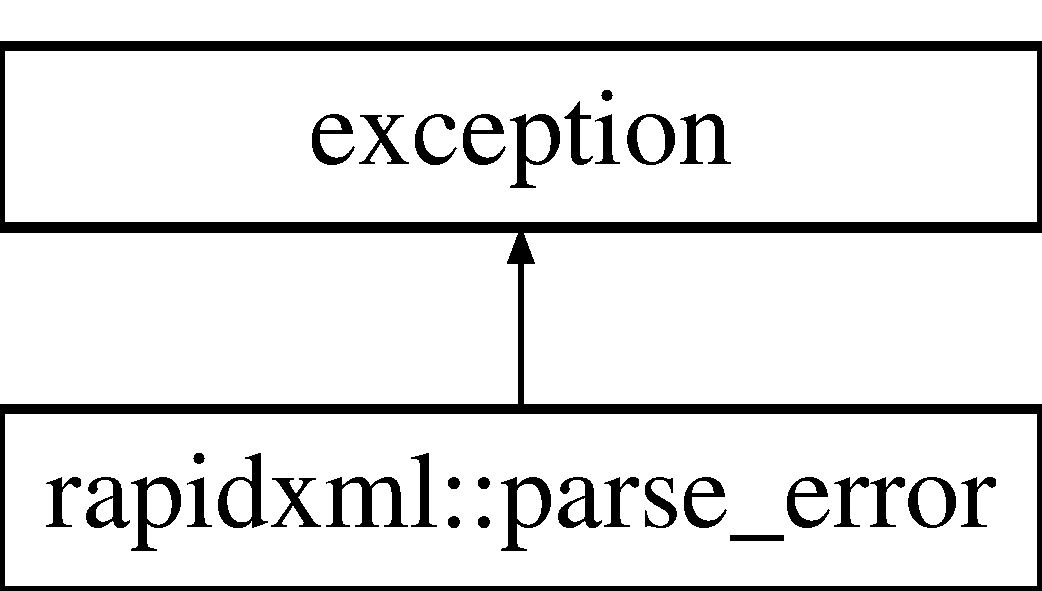
\includegraphics[height=2.000000cm]{classrapidxml_1_1parse__error}
\end{center}
\end{figure}
\subsection*{Public Member Functions}
\begin{DoxyCompactItemize}
\item 
\mbox{\Hypertarget{classrapidxml_1_1parse__error_aea12a301271c393fb627b368fb9f35c1}\label{classrapidxml_1_1parse__error_aea12a301271c393fb627b368fb9f35c1}} 
\mbox{\hyperlink{classrapidxml_1_1parse__error_aea12a301271c393fb627b368fb9f35c1}{parse\+\_\+error}} (const char $\ast$\mbox{\hyperlink{classrapidxml_1_1parse__error_a986003116ebcb49a69a20228da306232}{what}}, void $\ast$\mbox{\hyperlink{classrapidxml_1_1parse__error_ab139528f4d9e960f0ee807d22d6c032d}{where}})
\begin{DoxyCompactList}\small\item\em Constructs parse error. \end{DoxyCompactList}\item 
virtual const char $\ast$ \mbox{\hyperlink{classrapidxml_1_1parse__error_a986003116ebcb49a69a20228da306232}{what}} () const  throw ()
\item 
{\footnotesize template$<$class Ch $>$ }\\Ch $\ast$ \mbox{\hyperlink{classrapidxml_1_1parse__error_ab139528f4d9e960f0ee807d22d6c032d}{where}} () const
\end{DoxyCompactItemize}


\subsection{Detailed Description}
Parse error exception. This exception is thrown by the parser when an error occurs. Use \mbox{\hyperlink{classrapidxml_1_1parse__error_a986003116ebcb49a69a20228da306232}{what()}} function to get human-\/readable error message. Use \mbox{\hyperlink{classrapidxml_1_1parse__error_ab139528f4d9e960f0ee807d22d6c032d}{where()}} function to get a pointer to position within source text where error was detected. ~\newline
~\newline
 If throwing exceptions by the parser is undesirable, it can be disabled by defining R\+A\+P\+I\+D\+X\+M\+L\+\_\+\+N\+O\+\_\+\+E\+X\+C\+E\+P\+T\+I\+O\+NS macro before \mbox{\hyperlink{rapidxml_8hpp}{rapidxml.\+hpp}} is included. This will cause the parser to call rapidxml\+::parse\+\_\+error\+\_\+handler() function instead of throwing an exception. This function must be defined by the user. ~\newline
~\newline
 This class derives from {\ttfamily std\+::exception} class. 

\subsection{Member Function Documentation}
\mbox{\Hypertarget{classrapidxml_1_1parse__error_a986003116ebcb49a69a20228da306232}\label{classrapidxml_1_1parse__error_a986003116ebcb49a69a20228da306232}} 
\index{rapidxml\+::parse\+\_\+error@{rapidxml\+::parse\+\_\+error}!what@{what}}
\index{what@{what}!rapidxml\+::parse\+\_\+error@{rapidxml\+::parse\+\_\+error}}
\subsubsection{\texorpdfstring{what()}{what()}}
{\footnotesize\ttfamily virtual const char$\ast$ rapidxml\+::parse\+\_\+error\+::what (\begin{DoxyParamCaption}{ }\end{DoxyParamCaption}) const throw  ) \hspace{0.3cm}{\ttfamily [inline]}, {\ttfamily [virtual]}}

Gets human readable description of error. \begin{DoxyReturn}{Returns}
Pointer to null terminated description of the error. 
\end{DoxyReturn}
\mbox{\Hypertarget{classrapidxml_1_1parse__error_ab139528f4d9e960f0ee807d22d6c032d}\label{classrapidxml_1_1parse__error_ab139528f4d9e960f0ee807d22d6c032d}} 
\index{rapidxml\+::parse\+\_\+error@{rapidxml\+::parse\+\_\+error}!where@{where}}
\index{where@{where}!rapidxml\+::parse\+\_\+error@{rapidxml\+::parse\+\_\+error}}
\subsubsection{\texorpdfstring{where()}{where()}}
{\footnotesize\ttfamily template$<$class Ch $>$ \\
Ch$\ast$ rapidxml\+::parse\+\_\+error\+::where (\begin{DoxyParamCaption}{ }\end{DoxyParamCaption}) const\hspace{0.3cm}{\ttfamily [inline]}}

Gets pointer to character data where error happened. Ch should be the same as char type of \mbox{\hyperlink{classrapidxml_1_1xml__document}{xml\+\_\+document}} that produced the error. \begin{DoxyReturn}{Returns}
Pointer to location within the parsed string where error occured. 
\end{DoxyReturn}


The documentation for this class was generated from the following file\+:\begin{DoxyCompactItemize}
\item 
\mbox{\hyperlink{rapidxml_8hpp}{rapidxml.\+hpp}}\end{DoxyCompactItemize}

\hypertarget{classtfp_1_1_player}{}\section{tfp\+:\+:Player Class Reference}
\label{classtfp_1_1_player}\index{tfp\+::\+Player@{tfp\+::\+Player}}
Inheritance diagram for tfp\+:\+:Player\+:\begin{figure}[H]
\begin{center}
\leavevmode
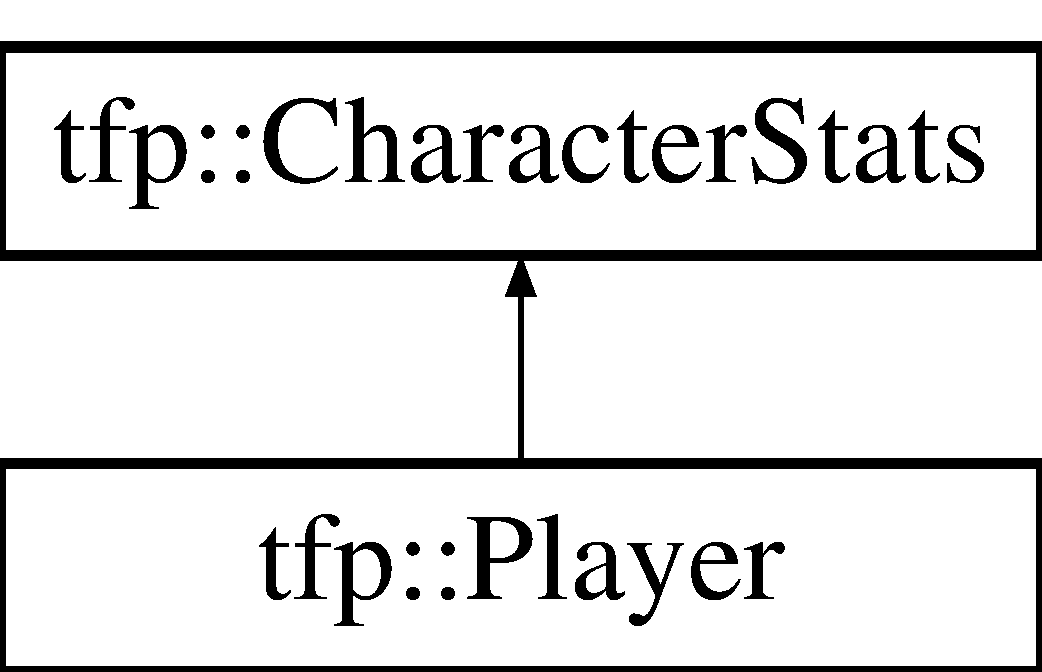
\includegraphics[height=2.000000cm]{classtfp_1_1_player}
\end{center}
\end{figure}
\subsection*{Public Member Functions}
\begin{DoxyCompactItemize}
\item 
\mbox{\Hypertarget{classtfp_1_1_player_aae80e75bc3d8b71256a8176e65e393b3}\label{classtfp_1_1_player_aae80e75bc3d8b71256a8176e65e393b3}} 
\mbox{\hyperlink{classtfp_1_1_player_aae80e75bc3d8b71256a8176e65e393b3}{Player}} ()
\begin{DoxyCompactList}\small\item\em Konstruktor. \end{DoxyCompactList}\item 
\mbox{\Hypertarget{classtfp_1_1_player_a9dd38f70e000bf5596636b55fd326e04}\label{classtfp_1_1_player_a9dd38f70e000bf5596636b55fd326e04}} 
\mbox{\hyperlink{classtfp_1_1_player_a9dd38f70e000bf5596636b55fd326e04}{$\sim$\+Player}} ()
\begin{DoxyCompactList}\small\item\em Destruktor. \end{DoxyCompactList}\item 
\mbox{\Hypertarget{classtfp_1_1_player_a9e18ed6b2335d4f7206260f7d6cb3a87}\label{classtfp_1_1_player_a9e18ed6b2335d4f7206260f7d6cb3a87}} 
void \mbox{\hyperlink{classtfp_1_1_player_a9e18ed6b2335d4f7206260f7d6cb3a87}{Set\+ID}} (int ID)
\begin{DoxyCompactList}\small\item\em Ustawia id gracza. \end{DoxyCompactList}\item 
\mbox{\Hypertarget{classtfp_1_1_player_aa21e13d6c0d6e44c40344aa1e31f2b4e}\label{classtfp_1_1_player_aa21e13d6c0d6e44c40344aa1e31f2b4e}} 
int \mbox{\hyperlink{classtfp_1_1_player_aa21e13d6c0d6e44c40344aa1e31f2b4e}{Get\+ID}} ()
\begin{DoxyCompactList}\small\item\em Zwraca id gracza. \end{DoxyCompactList}\item 
\mbox{\Hypertarget{classtfp_1_1_player_a18013b7cf6924783094eeb7db0d1cc15}\label{classtfp_1_1_player_a18013b7cf6924783094eeb7db0d1cc15}} 
void \mbox{\hyperlink{classtfp_1_1_player_a18013b7cf6924783094eeb7db0d1cc15}{Set\+Name}} (std\+::string Name)
\begin{DoxyCompactList}\small\item\em Ustawia nazwe gracza. \end{DoxyCompactList}\item 
\mbox{\Hypertarget{classtfp_1_1_player_a967236fb7eef441d4cc98df554063bd2}\label{classtfp_1_1_player_a967236fb7eef441d4cc98df554063bd2}} 
std\+::string \mbox{\hyperlink{classtfp_1_1_player_a967236fb7eef441d4cc98df554063bd2}{Get\+Name}} ()
\begin{DoxyCompactList}\small\item\em Zwraca nazwe gracza. \end{DoxyCompactList}\item 
\mbox{\Hypertarget{classtfp_1_1_player_a589d31655ef8300f48f093c893e78f77}\label{classtfp_1_1_player_a589d31655ef8300f48f093c893e78f77}} 
void \mbox{\hyperlink{classtfp_1_1_player_a589d31655ef8300f48f093c893e78f77}{Set\+Skin\+Name}} (std\+::string Skin\+Name)
\begin{DoxyCompactList}\small\item\em Ustawia nazwe skina. \end{DoxyCompactList}\item 
\mbox{\Hypertarget{classtfp_1_1_player_a34290c1644107a6db7946bbfdc11538c}\label{classtfp_1_1_player_a34290c1644107a6db7946bbfdc11538c}} 
std\+::string \mbox{\hyperlink{classtfp_1_1_player_a34290c1644107a6db7946bbfdc11538c}{Get\+Skin\+Name}} ()
\begin{DoxyCompactList}\small\item\em Zwraca nazwe skina. \end{DoxyCompactList}\item 
\mbox{\Hypertarget{classtfp_1_1_player_ab25c921fda17930eaf2bc763ef1040ff}\label{classtfp_1_1_player_ab25c921fda17930eaf2bc763ef1040ff}} 
void \mbox{\hyperlink{classtfp_1_1_player_ab25c921fda17930eaf2bc763ef1040ff}{Set\+Position}} (sf\+::\+Vector2f Position)
\begin{DoxyCompactList}\small\item\em Ustawia pozycje gracza. \end{DoxyCompactList}\item 
\mbox{\Hypertarget{classtfp_1_1_player_ac8aa30878427c31b9da1d9bf114e6a75}\label{classtfp_1_1_player_ac8aa30878427c31b9da1d9bf114e6a75}} 
sf\+::\+Vector2f \mbox{\hyperlink{classtfp_1_1_player_ac8aa30878427c31b9da1d9bf114e6a75}{Get\+Position}} ()
\begin{DoxyCompactList}\small\item\em Zwraca pozycje gracza. \end{DoxyCompactList}\item 
\mbox{\Hypertarget{classtfp_1_1_player_a849b97e1007d2e234ce17d106681a992}\label{classtfp_1_1_player_a849b97e1007d2e234ce17d106681a992}} 
void \mbox{\hyperlink{classtfp_1_1_player_a849b97e1007d2e234ce17d106681a992}{Set\+Destination}} (sf\+::\+Vector2f Destination)
\begin{DoxyCompactList}\small\item\em Ustawia pozycje docelowa gracza. \end{DoxyCompactList}\item 
\mbox{\Hypertarget{classtfp_1_1_player_a9a6550ba33abab92ad6cbf35ee3c9174}\label{classtfp_1_1_player_a9a6550ba33abab92ad6cbf35ee3c9174}} 
sf\+::\+Vector2f \mbox{\hyperlink{classtfp_1_1_player_a9a6550ba33abab92ad6cbf35ee3c9174}{Get\+Destination}} ()
\begin{DoxyCompactList}\small\item\em Zwraca pozycje docelowa gracza. \end{DoxyCompactList}\item 
\mbox{\Hypertarget{classtfp_1_1_player_a1cf97652344d339f9d920f71caf3761c}\label{classtfp_1_1_player_a1cf97652344d339f9d920f71caf3761c}} 
void \mbox{\hyperlink{classtfp_1_1_player_a1cf97652344d339f9d920f71caf3761c}{Set\+Boost\+Speed}} (float Speed)
\begin{DoxyCompactList}\small\item\em Ustawia boost do szbkosci poruszania. \end{DoxyCompactList}\item 
\mbox{\Hypertarget{classtfp_1_1_player_ad344b1e188d18cdf03e63a90e5224da0}\label{classtfp_1_1_player_ad344b1e188d18cdf03e63a90e5224da0}} 
float \mbox{\hyperlink{classtfp_1_1_player_ad344b1e188d18cdf03e63a90e5224da0}{Get\+Boost\+Speed}} ()
\begin{DoxyCompactList}\small\item\em Zwraca boost do szybkosci poruszania. \end{DoxyCompactList}\item 
\mbox{\Hypertarget{classtfp_1_1_player_a414ca8c7b9693aba5e2d510e3b46173d}\label{classtfp_1_1_player_a414ca8c7b9693aba5e2d510e3b46173d}} 
void \mbox{\hyperlink{classtfp_1_1_player_a414ca8c7b9693aba5e2d510e3b46173d}{Set\+Looking\+Direction}} (tfp\+::\+Direction Looking\+Direction)
\begin{DoxyCompactList}\small\item\em Ustawia kierunek parzenia gracza. \end{DoxyCompactList}\item 
\mbox{\Hypertarget{classtfp_1_1_player_a4ebb4b5f4f47e13a3bae50ab99ddfdc7}\label{classtfp_1_1_player_a4ebb4b5f4f47e13a3bae50ab99ddfdc7}} 
tfp\+::\+Direction \mbox{\hyperlink{classtfp_1_1_player_a4ebb4b5f4f47e13a3bae50ab99ddfdc7}{Get\+Looking\+Direction}} ()
\begin{DoxyCompactList}\small\item\em Zwraca kierunek patrzenia gracza. \end{DoxyCompactList}\item 
\mbox{\Hypertarget{classtfp_1_1_player_a2e1f8245e3248349e75d065ccac3b747}\label{classtfp_1_1_player_a2e1f8245e3248349e75d065ccac3b747}} 
void \mbox{\hyperlink{classtfp_1_1_player_a2e1f8245e3248349e75d065ccac3b747}{Set\+Level}} (int Level)
\begin{DoxyCompactList}\small\item\em Ustawia posiom. \end{DoxyCompactList}\item 
\mbox{\Hypertarget{classtfp_1_1_player_aadfd30b570e52a5482759a5f8a13dac1}\label{classtfp_1_1_player_aadfd30b570e52a5482759a5f8a13dac1}} 
int \mbox{\hyperlink{classtfp_1_1_player_aadfd30b570e52a5482759a5f8a13dac1}{Get\+Level}} ()
\begin{DoxyCompactList}\small\item\em Zwraca poziom. \end{DoxyCompactList}\item 
\mbox{\Hypertarget{classtfp_1_1_player_aec49ecba2508ef77b0a3f436024e1933}\label{classtfp_1_1_player_aec49ecba2508ef77b0a3f436024e1933}} 
void \mbox{\hyperlink{classtfp_1_1_player_aec49ecba2508ef77b0a3f436024e1933}{Set\+Experience}} (int Experience)
\begin{DoxyCompactList}\small\item\em Ustawia doswiadczenie. \end{DoxyCompactList}\item 
\mbox{\Hypertarget{classtfp_1_1_player_ad42d94d800dfd5e4443e46e65eae3b8f}\label{classtfp_1_1_player_ad42d94d800dfd5e4443e46e65eae3b8f}} 
int \mbox{\hyperlink{classtfp_1_1_player_ad42d94d800dfd5e4443e46e65eae3b8f}{Get\+Experience}} ()
\begin{DoxyCompactList}\small\item\em Zwraca doswiadczenie. \end{DoxyCompactList}\item 
\mbox{\Hypertarget{classtfp_1_1_player_acabdb43e354fc56e0ae31237a27cb391}\label{classtfp_1_1_player_acabdb43e354fc56e0ae31237a27cb391}} 
void \mbox{\hyperlink{classtfp_1_1_player_acabdb43e354fc56e0ae31237a27cb391}{Set\+Inventory\+Size}} (int Width, int Height)
\begin{DoxyCompactList}\small\item\em Ustawia rozmiar ekwipunku. \end{DoxyCompactList}\item 
\mbox{\Hypertarget{classtfp_1_1_player_adac483d955774193b8c786e88c3a069a}\label{classtfp_1_1_player_adac483d955774193b8c786e88c3a069a}} 
void \mbox{\hyperlink{classtfp_1_1_player_adac483d955774193b8c786e88c3a069a}{Set\+Inventory\+Size}} (sf\+::\+Vector2i Size)
\begin{DoxyCompactList}\small\item\em Ustawia rozmiar ekwipunku. \end{DoxyCompactList}\item 
\mbox{\Hypertarget{classtfp_1_1_player_a348f5b369f74c2268982709e3162cd5f}\label{classtfp_1_1_player_a348f5b369f74c2268982709e3162cd5f}} 
sf\+::\+Vector2i \mbox{\hyperlink{classtfp_1_1_player_a348f5b369f74c2268982709e3162cd5f}{Get\+Inventory\+Size}} ()
\begin{DoxyCompactList}\small\item\em Zwraca rozmiar ekwipunku. \end{DoxyCompactList}\item 
\mbox{\Hypertarget{classtfp_1_1_player_ababfde32d562d636214faa86a5006c8b}\label{classtfp_1_1_player_ababfde32d562d636214faa86a5006c8b}} 
void \mbox{\hyperlink{classtfp_1_1_player_ababfde32d562d636214faa86a5006c8b}{Set\+Inventory\+Item}} (std\+::string Name, int Quantity, int List\+Position)
\begin{DoxyCompactList}\small\item\em Ustawia przedmiot w ekwipunku w wybranym miejscu. \end{DoxyCompactList}\end{DoxyCompactItemize}
\subsection*{Public Attributes}
\begin{DoxyCompactItemize}
\item 
\mbox{\Hypertarget{classtfp_1_1_player_a3c6707ea108f52cbbff9d396c93d6fdb}\label{classtfp_1_1_player_a3c6707ea108f52cbbff9d396c93d6fdb}} 
std\+::vector$<$ \mbox{\hyperlink{structtfp_1_1_item}{tfp\+::\+Item}} $>$ {\bfseries Inventory\+Item\+List}
\end{DoxyCompactItemize}


The documentation for this class was generated from the following files\+:\begin{DoxyCompactItemize}
\item 
character.\+hpp\item 
character.\+cpp\end{DoxyCompactItemize}

\hypertarget{classtfp_1_1specialeffects_1_1_rain}{}\section{tfp\+:\+:specialeffects\+:\+:Rain Class Reference}
\label{classtfp_1_1specialeffects_1_1_rain}\index{tfp\+::specialeffects\+::\+Rain@{tfp\+::specialeffects\+::\+Rain}}
\subsection*{Public Member Functions}
\begin{DoxyCompactItemize}
\item 
\mbox{\Hypertarget{classtfp_1_1specialeffects_1_1_rain_ab9fbf8d201b9f71d40d6a0c2a3effe22}\label{classtfp_1_1specialeffects_1_1_rain_ab9fbf8d201b9f71d40d6a0c2a3effe22}} 
\mbox{\hyperlink{classtfp_1_1specialeffects_1_1_rain_ab9fbf8d201b9f71d40d6a0c2a3effe22}{Rain}} ()
\begin{DoxyCompactList}\small\item\em Constructor. \end{DoxyCompactList}\item 
\mbox{\Hypertarget{classtfp_1_1specialeffects_1_1_rain_acdac171c8522ef034f94413ba181771f}\label{classtfp_1_1specialeffects_1_1_rain_acdac171c8522ef034f94413ba181771f}} 
\mbox{\hyperlink{classtfp_1_1specialeffects_1_1_rain_acdac171c8522ef034f94413ba181771f}{$\sim$\+Rain}} ()
\begin{DoxyCompactList}\small\item\em Destructor. \end{DoxyCompactList}\item 
\mbox{\Hypertarget{classtfp_1_1specialeffects_1_1_rain_ac317a6cfc99d95a3dc53e85f0b0e4d69}\label{classtfp_1_1specialeffects_1_1_rain_ac317a6cfc99d95a3dc53e85f0b0e4d69}} 
void \mbox{\hyperlink{classtfp_1_1specialeffects_1_1_rain_ac317a6cfc99d95a3dc53e85f0b0e4d69}{Set\+Game\+Handle}} (\mbox{\hyperlink{classtfp_1_1_game}{tfp\+::\+Game}} $\ast$Handle)
\begin{DoxyCompactList}\small\item\em Sets game handle. \end{DoxyCompactList}\item 
void \mbox{\hyperlink{classtfp_1_1specialeffects_1_1_rain_a5a0baf62d50003eda4af4da3ebb0f0ee}{Display}} ()
\begin{DoxyCompactList}\small\item\em Render rain. \end{DoxyCompactList}\item 
\mbox{\Hypertarget{classtfp_1_1specialeffects_1_1_rain_a8dc0d21ff7b21eab4c741699c5216dd0}\label{classtfp_1_1specialeffects_1_1_rain_a8dc0d21ff7b21eab4c741699c5216dd0}} 
void \mbox{\hyperlink{classtfp_1_1specialeffects_1_1_rain_a8dc0d21ff7b21eab4c741699c5216dd0}{Set\+Density}} (int Value)
\begin{DoxyCompactList}\small\item\em Sets rain density (how much rain drops spawns in a given time) \end{DoxyCompactList}\item 
\mbox{\Hypertarget{classtfp_1_1specialeffects_1_1_rain_a9f28f426b054f8a7028addb8b74159d8}\label{classtfp_1_1specialeffects_1_1_rain_a9f28f426b054f8a7028addb8b74159d8}} 
void \mbox{\hyperlink{classtfp_1_1specialeffects_1_1_rain_a9f28f426b054f8a7028addb8b74159d8}{Set\+Creation\+Speed}} (float Time\+Between\+Creation)
\begin{DoxyCompactList}\small\item\em Sets time betwen creating new rain drops. \end{DoxyCompactList}\item 
\mbox{\Hypertarget{classtfp_1_1specialeffects_1_1_rain_ad74727aa55ddfcc25adb7b222068b935}\label{classtfp_1_1specialeffects_1_1_rain_ad74727aa55ddfcc25adb7b222068b935}} 
void \mbox{\hyperlink{classtfp_1_1specialeffects_1_1_rain_ad74727aa55ddfcc25adb7b222068b935}{Set\+Fall\+Speed}} (float Speed)
\begin{DoxyCompactList}\small\item\em Sets speed of falling rain. \end{DoxyCompactList}\end{DoxyCompactItemize}


\subsection{Member Function Documentation}
\mbox{\Hypertarget{classtfp_1_1specialeffects_1_1_rain_a5a0baf62d50003eda4af4da3ebb0f0ee}\label{classtfp_1_1specialeffects_1_1_rain_a5a0baf62d50003eda4af4da3ebb0f0ee}} 
\index{tfp\+::specialeffects\+::\+Rain@{tfp\+::specialeffects\+::\+Rain}!Display@{Display}}
\index{Display@{Display}!tfp\+::specialeffects\+::\+Rain@{tfp\+::specialeffects\+::\+Rain}}
\subsubsection{\texorpdfstring{Display()}{Display()}}
{\footnotesize\ttfamily void tfp\+::specialeffects\+::\+Rain\+::\+Display (\begin{DoxyParamCaption}{ }\end{DoxyParamCaption})}



Render rain. 

Tworzenie

Przesuwanie i zabijanie

Drop\+List\mbox{[}i\mbox{]}.Life\+Span $\ast$ 0.\+002f ~\newline
 Renderowanie 

The documentation for this class was generated from the following files\+:\begin{DoxyCompactItemize}
\item 
interfaceffects.\+hpp\item 
interfaceffects.\+cpp\end{DoxyCompactItemize}

\hypertarget{classtfp_1_1_screen}{}\section{tfp\+:\+:Screen Class Reference}
\label{classtfp_1_1_screen}\index{tfp\+::\+Screen@{tfp\+::\+Screen}}
\subsection*{Public Member Functions}
\begin{DoxyCompactItemize}
\item 
\mbox{\hyperlink{classtfp_1_1_screen_a8a5d28db3e41c9e816dc1ea6a6aa9a81}{Screen}} ()
\begin{DoxyCompactList}\small\item\em Konstruktor. \end{DoxyCompactList}\item 
\mbox{\Hypertarget{classtfp_1_1_screen_ace30a792f8887193324d999b5686cae3}\label{classtfp_1_1_screen_ace30a792f8887193324d999b5686cae3}} 
\mbox{\hyperlink{classtfp_1_1_screen_ace30a792f8887193324d999b5686cae3}{$\sim$\+Screen}} ()
\begin{DoxyCompactList}\small\item\em Destruktor. \end{DoxyCompactList}\item 
\mbox{\Hypertarget{classtfp_1_1_screen_a67d43bfb9e822042feb60457e915c9ff}\label{classtfp_1_1_screen_a67d43bfb9e822042feb60457e915c9ff}} 
void \mbox{\hyperlink{classtfp_1_1_screen_a67d43bfb9e822042feb60457e915c9ff}{Display\+Window}} ()
\begin{DoxyCompactList}\small\item\em Wyswietla okno i obsluguje wszystkie zdarzenia. \end{DoxyCompactList}\item 
\mbox{\Hypertarget{classtfp_1_1_screen_a63867d99a2023ca238375281c8b810f0}\label{classtfp_1_1_screen_a63867d99a2023ca238375281c8b810f0}} 
const bool \mbox{\hyperlink{classtfp_1_1_screen_a63867d99a2023ca238375281c8b810f0}{Is\+Window\+Open}} ()
\begin{DoxyCompactList}\small\item\em Czy okno jest otwarte. \end{DoxyCompactList}\item 
\mbox{\Hypertarget{classtfp_1_1_screen_abf2439c27caf3e12742a5d1f6f4e6c55}\label{classtfp_1_1_screen_abf2439c27caf3e12742a5d1f6f4e6c55}} 
void \mbox{\hyperlink{classtfp_1_1_screen_abf2439c27caf3e12742a5d1f6f4e6c55}{Draw}} (const sf\+::\+Drawable \&Drawable)
\begin{DoxyCompactList}\small\item\em Rysowanie w oknie. \end{DoxyCompactList}\item 
\mbox{\Hypertarget{classtfp_1_1_screen_a137bcd621d06eae9a53d743f8c6ad135}\label{classtfp_1_1_screen_a137bcd621d06eae9a53d743f8c6ad135}} 
void \mbox{\hyperlink{classtfp_1_1_screen_a137bcd621d06eae9a53d743f8c6ad135}{Draw\+Vertex}} (const sf\+::\+Vertex $\ast$vertices, std\+::size\+\_\+t vertex\+Count, sf\+::\+Primitive\+Type type, const sf\+::\+Render\+States \&states=sf\+::\+Render\+States\+::\+Default)
\begin{DoxyCompactList}\small\item\em Rysowanie w oknie. \end{DoxyCompactList}\item 
\mbox{\Hypertarget{classtfp_1_1_screen_a9c1b0e49638812235f547e5c6c8b4789}\label{classtfp_1_1_screen_a9c1b0e49638812235f547e5c6c8b4789}} 
void \mbox{\hyperlink{classtfp_1_1_screen_a9c1b0e49638812235f547e5c6c8b4789}{Clear}} ()
\begin{DoxyCompactList}\small\item\em Wyczysc. \end{DoxyCompactList}\item 
\mbox{\Hypertarget{classtfp_1_1_screen_a6ca9681484ed2c404beb13c437138676}\label{classtfp_1_1_screen_a6ca9681484ed2c404beb13c437138676}} 
sf\+::\+Event \mbox{\hyperlink{classtfp_1_1_screen_a6ca9681484ed2c404beb13c437138676}{Get\+Screen\+Event}} ()
\begin{DoxyCompactList}\small\item\em Pobieranie eventow ze screen. \end{DoxyCompactList}\item 
\mbox{\Hypertarget{classtfp_1_1_screen_a9f224862fc68528caa4cc1f5fb73f013}\label{classtfp_1_1_screen_a9f224862fc68528caa4cc1f5fb73f013}} 
const bool {\bfseries Is\+Event\+In\+Queue} ()
\item 
\mbox{\Hypertarget{classtfp_1_1_screen_a11e80d123390d4713b4b7ba49a5af393}\label{classtfp_1_1_screen_a11e80d123390d4713b4b7ba49a5af393}} 
void \mbox{\hyperlink{classtfp_1_1_screen_a11e80d123390d4713b4b7ba49a5af393}{Close}} ()
\begin{DoxyCompactList}\small\item\em Zamykanie okna. \end{DoxyCompactList}\item 
\mbox{\Hypertarget{classtfp_1_1_screen_aa27dec08639e5aadcdce2af3674db316}\label{classtfp_1_1_screen_aa27dec08639e5aadcdce2af3674db316}} 
const bool \& \mbox{\hyperlink{classtfp_1_1_screen_aa27dec08639e5aadcdce2af3674db316}{Is\+Focused}} () const
\begin{DoxyCompactList}\small\item\em Czy jest aktywne okno. \end{DoxyCompactList}\item 
\mbox{\Hypertarget{classtfp_1_1_screen_af2f7112d8498bb2ee538929e6c96921d}\label{classtfp_1_1_screen_af2f7112d8498bb2ee538929e6c96921d}} 
void \mbox{\hyperlink{classtfp_1_1_screen_af2f7112d8498bb2ee538929e6c96921d}{Set\+Focus}} (bool State)
\begin{DoxyCompactList}\small\item\em Ustawia focus okna. \end{DoxyCompactList}\item 
\mbox{\Hypertarget{classtfp_1_1_screen_a4b985b553b9592d774226fc4edc5488c}\label{classtfp_1_1_screen_a4b985b553b9592d774226fc4edc5488c}} 
const int \mbox{\hyperlink{classtfp_1_1_screen_a4b985b553b9592d774226fc4edc5488c}{Get\+Framerate\+Limit}} () const
\begin{DoxyCompactList}\small\item\em Pobiera limit klatek;. \end{DoxyCompactList}\item 
\mbox{\Hypertarget{classtfp_1_1_screen_a1cdd94f37e5f93003e2e1026fb204aec}\label{classtfp_1_1_screen_a1cdd94f37e5f93003e2e1026fb204aec}} 
sf\+::\+Render\+Window \& \mbox{\hyperlink{classtfp_1_1_screen_a1cdd94f37e5f93003e2e1026fb204aec}{Get\+Render\+Window\+Handle}} ()
\begin{DoxyCompactList}\small\item\em Uzywac tylko w funkcjach sfml. \end{DoxyCompactList}\item 
\mbox{\Hypertarget{classtfp_1_1_screen_a840bee6a6f3f201da6daa388ff15e850}\label{classtfp_1_1_screen_a840bee6a6f3f201da6daa388ff15e850}} 
const sf\+::\+Vector2i \mbox{\hyperlink{classtfp_1_1_screen_a840bee6a6f3f201da6daa388ff15e850}{Get\+Window\+Size}} ()
\begin{DoxyCompactList}\small\item\em Wymiary okna. \end{DoxyCompactList}\item 
\mbox{\Hypertarget{classtfp_1_1_screen_a88b2486f29909286c7388328722414d2}\label{classtfp_1_1_screen_a88b2486f29909286c7388328722414d2}} 
const sf\+::\+Vector2i \mbox{\hyperlink{classtfp_1_1_screen_a88b2486f29909286c7388328722414d2}{Get\+View\+Size}} ()
\begin{DoxyCompactList}\small\item\em Wymiary widoku. \end{DoxyCompactList}\item 
\mbox{\Hypertarget{classtfp_1_1_screen_ab6ba51ac1063ed7b9cab2195065887f2}\label{classtfp_1_1_screen_ab6ba51ac1063ed7b9cab2195065887f2}} 
const sf\+::\+Vector2i \mbox{\hyperlink{classtfp_1_1_screen_ab6ba51ac1063ed7b9cab2195065887f2}{Get\+Original\+View\+Size}} ()
\begin{DoxyCompactList}\small\item\em Wymiary oryginalne widoku. \end{DoxyCompactList}\item 
\mbox{\Hypertarget{classtfp_1_1_screen_a19f350b2ef7e30842d2d582976034215}\label{classtfp_1_1_screen_a19f350b2ef7e30842d2d582976034215}} 
void \mbox{\hyperlink{classtfp_1_1_screen_a19f350b2ef7e30842d2d582976034215}{Set\+View\+Scale}} (float Scale)
\begin{DoxyCompactList}\small\item\em Zmiana skali widoku. \end{DoxyCompactList}\item 
\mbox{\Hypertarget{classtfp_1_1_screen_a064c5c3f3d83d229a9d66df1c9bd1054}\label{classtfp_1_1_screen_a064c5c3f3d83d229a9d66df1c9bd1054}} 
void \mbox{\hyperlink{classtfp_1_1_screen_a064c5c3f3d83d229a9d66df1c9bd1054}{Resize}} (int Width, int Height, bool Full\+Screen)
\begin{DoxyCompactList}\small\item\em Zmiana rozmiaru okna. \end{DoxyCompactList}\item 
\mbox{\Hypertarget{classtfp_1_1_screen_ab432ae70eebd86b018d9d1d21cf3abb2}\label{classtfp_1_1_screen_ab432ae70eebd86b018d9d1d21cf3abb2}} 
void \mbox{\hyperlink{classtfp_1_1_screen_ab432ae70eebd86b018d9d1d21cf3abb2}{Resize}} ()
\begin{DoxyCompactList}\small\item\em Reset rozmiaru okna. \end{DoxyCompactList}\item 
\mbox{\Hypertarget{classtfp_1_1_screen_ad9257fe04dff4799034d400139d551fb}\label{classtfp_1_1_screen_ad9257fe04dff4799034d400139d551fb}} 
void \mbox{\hyperlink{classtfp_1_1_screen_ad9257fe04dff4799034d400139d551fb}{Set\+View\+Size}} (int Width, int Height)
\begin{DoxyCompactList}\small\item\em Zmiana rozmiaru widoku. \end{DoxyCompactList}\item 
\mbox{\Hypertarget{classtfp_1_1_screen_a291e2adea82570ac89dd57fba8674fdf}\label{classtfp_1_1_screen_a291e2adea82570ac89dd57fba8674fdf}} 
const float \mbox{\hyperlink{classtfp_1_1_screen_a291e2adea82570ac89dd57fba8674fdf}{Get\+View\+Scale}} ()
\begin{DoxyCompactList}\small\item\em Zwraca skale zmienionej przez komendy do oryginalnej rozdzielczosci. \end{DoxyCompactList}\item 
\mbox{\Hypertarget{classtfp_1_1_screen_a134be9e36c0ff4761fe81d25045f4806}\label{classtfp_1_1_screen_a134be9e36c0ff4761fe81d25045f4806}} 
void \mbox{\hyperlink{classtfp_1_1_screen_a134be9e36c0ff4761fe81d25045f4806}{Set\+Window\+Title}} (std\+::wstring Title)
\begin{DoxyCompactList}\small\item\em Zmienia nazwe okna. \end{DoxyCompactList}\item 
\mbox{\Hypertarget{classtfp_1_1_screen_a7e3775842c52977385ab5d98ba0bf31d}\label{classtfp_1_1_screen_a7e3775842c52977385ab5d98ba0bf31d}} 
void \mbox{\hyperlink{classtfp_1_1_screen_a7e3775842c52977385ab5d98ba0bf31d}{Set\+Game\+Handle}} (\mbox{\hyperlink{classtfp_1_1_game}{tfp\+::\+Game}} $\ast$Handle)
\begin{DoxyCompactList}\small\item\em Ustawia wskacnik gry. \end{DoxyCompactList}\item 
\mbox{\Hypertarget{classtfp_1_1_screen_a81bf8070d65936fb5dd3a0b186137ea0}\label{classtfp_1_1_screen_a81bf8070d65936fb5dd3a0b186137ea0}} 
bool \mbox{\hyperlink{classtfp_1_1_screen_a81bf8070d65936fb5dd3a0b186137ea0}{Get\+Full\+Screen}} (std\+::string Game\+Type)
\begin{DoxyCompactList}\small\item\em Zwraca czy pelny ekran jest wlaczony w wybranym oknie gry. \end{DoxyCompactList}\item 
\mbox{\Hypertarget{classtfp_1_1_screen_a35c1f8551d84675694a0b3fc06161dee}\label{classtfp_1_1_screen_a35c1f8551d84675694a0b3fc06161dee}} 
void \mbox{\hyperlink{classtfp_1_1_screen_a35c1f8551d84675694a0b3fc06161dee}{Set\+Full\+Screen}} (std\+::string Game\+Type, bool State)
\begin{DoxyCompactList}\small\item\em Ustawia pelny ekran w wybranym oknie gry. \end{DoxyCompactList}\item 
\mbox{\Hypertarget{classtfp_1_1_screen_a7fef3437450fa6e50642793beed28081}\label{classtfp_1_1_screen_a7fef3437450fa6e50642793beed28081}} 
void \mbox{\hyperlink{classtfp_1_1_screen_a7fef3437450fa6e50642793beed28081}{Set\+Window\+Size}} (std\+::string Game\+Type, int New\+Width, int New\+Height)
\begin{DoxyCompactList}\small\item\em Ustawia rozmiar wybranego okna. \end{DoxyCompactList}\item 
\mbox{\Hypertarget{classtfp_1_1_screen_a772f3f5d508d716152c7193873100acd}\label{classtfp_1_1_screen_a772f3f5d508d716152c7193873100acd}} 
void \mbox{\hyperlink{classtfp_1_1_screen_a772f3f5d508d716152c7193873100acd}{Save\+Settings}} ()
\begin{DoxyCompactList}\small\item\em Zapisuje konfiguracje ustawien. \end{DoxyCompactList}\item 
\mbox{\Hypertarget{classtfp_1_1_screen_a1343043f5e05a5f623a231855ede76ae}\label{classtfp_1_1_screen_a1343043f5e05a5f623a231855ede76ae}} 
bool \mbox{\hyperlink{classtfp_1_1_screen_a1343043f5e05a5f623a231855ede76ae}{Get\+Vertical\+Sync}} ()
\begin{DoxyCompactList}\small\item\em Zwraca czy synchronizacja pionowa jest aktywna. \end{DoxyCompactList}\item 
\mbox{\Hypertarget{classtfp_1_1_screen_a6574eead04fbb2a4fa596fc8e6a19a81}\label{classtfp_1_1_screen_a6574eead04fbb2a4fa596fc8e6a19a81}} 
void \mbox{\hyperlink{classtfp_1_1_screen_a6574eead04fbb2a4fa596fc8e6a19a81}{Set\+Vertical\+Sync}} (bool State)
\begin{DoxyCompactList}\small\item\em Ustawia synchronizacje pionowa. \end{DoxyCompactList}\item 
\mbox{\Hypertarget{classtfp_1_1_screen_ad143e88307318b185382dc563c956cb2}\label{classtfp_1_1_screen_ad143e88307318b185382dc563c956cb2}} 
void \mbox{\hyperlink{classtfp_1_1_screen_ad143e88307318b185382dc563c956cb2}{Reset\+Settings}} ()
\begin{DoxyCompactList}\small\item\em Resetuje ustawienia. \end{DoxyCompactList}\end{DoxyCompactItemize}
\subsection*{Protected Attributes}
\begin{DoxyCompactItemize}
\item 
\mbox{\Hypertarget{classtfp_1_1_screen_a68859ed29c3e240fac1fca0920faeb5d}\label{classtfp_1_1_screen_a68859ed29c3e240fac1fca0920faeb5d}} 
int \mbox{\hyperlink{classtfp_1_1_screen_a68859ed29c3e240fac1fca0920faeb5d}{Menu\+Width}}
\begin{DoxyCompactList}\small\item\em Rozmiar okna. \end{DoxyCompactList}\item 
\mbox{\Hypertarget{classtfp_1_1_screen_a82692b112df068cf9ef727ca4cadc200}\label{classtfp_1_1_screen_a82692b112df068cf9ef727ca4cadc200}} 
int {\bfseries Game\+Width}
\item 
\mbox{\Hypertarget{classtfp_1_1_screen_a6599cdf153a9ccfd09d995dd26b421ec}\label{classtfp_1_1_screen_a6599cdf153a9ccfd09d995dd26b421ec}} 
int {\bfseries Map\+Editor\+Width}
\item 
\mbox{\Hypertarget{classtfp_1_1_screen_aa51f63d08fbded7e11c418012692fb0e}\label{classtfp_1_1_screen_aa51f63d08fbded7e11c418012692fb0e}} 
int {\bfseries Server\+Width}
\item 
\mbox{\Hypertarget{classtfp_1_1_screen_a468f094b9a0cd31767321773ff4ba312}\label{classtfp_1_1_screen_a468f094b9a0cd31767321773ff4ba312}} 
int {\bfseries Menu\+Height}
\item 
\mbox{\Hypertarget{classtfp_1_1_screen_a858c0dcb6d1da77e3f70743c18629c73}\label{classtfp_1_1_screen_a858c0dcb6d1da77e3f70743c18629c73}} 
int {\bfseries Game\+Height}
\item 
\mbox{\Hypertarget{classtfp_1_1_screen_a40a8c425ef0dc280bdd0c5eac03971d5}\label{classtfp_1_1_screen_a40a8c425ef0dc280bdd0c5eac03971d5}} 
int {\bfseries Map\+Editor\+Height}
\item 
\mbox{\Hypertarget{classtfp_1_1_screen_a9849da02386c868319f57a779caa6d11}\label{classtfp_1_1_screen_a9849da02386c868319f57a779caa6d11}} 
int {\bfseries Server\+Height}
\item 
\mbox{\Hypertarget{classtfp_1_1_screen_a67b21d9e724e9ba8b6e58fc50a88d168}\label{classtfp_1_1_screen_a67b21d9e724e9ba8b6e58fc50a88d168}} 
int \mbox{\hyperlink{classtfp_1_1_screen_a67b21d9e724e9ba8b6e58fc50a88d168}{View\+Width}}
\begin{DoxyCompactList}\small\item\em Rozmiar widoku. \end{DoxyCompactList}\item 
\mbox{\Hypertarget{classtfp_1_1_screen_ac94d98692dbfab35e2bbd6fd7047b8b1}\label{classtfp_1_1_screen_ac94d98692dbfab35e2bbd6fd7047b8b1}} 
int {\bfseries View\+Height}
\item 
\mbox{\Hypertarget{classtfp_1_1_screen_a49ee27e83c988eb0143eebf2b86f3345}\label{classtfp_1_1_screen_a49ee27e83c988eb0143eebf2b86f3345}} 
int {\bfseries View\+Original\+Width}
\item 
\mbox{\Hypertarget{classtfp_1_1_screen_aca50d096adc023b63c7675cb7be65beb}\label{classtfp_1_1_screen_aca50d096adc023b63c7675cb7be65beb}} 
int {\bfseries View\+Original\+Height}
\item 
\mbox{\Hypertarget{classtfp_1_1_screen_ab34d656b976b145fdeebf7a5b2635036}\label{classtfp_1_1_screen_ab34d656b976b145fdeebf7a5b2635036}} 
int \mbox{\hyperlink{classtfp_1_1_screen_ab34d656b976b145fdeebf7a5b2635036}{View\+Horizontal\+Center}}
\begin{DoxyCompactList}\small\item\em Srodek widoku. \end{DoxyCompactList}\item 
\mbox{\Hypertarget{classtfp_1_1_screen_a3ee23f2c207b80b458afa208b85eadaf}\label{classtfp_1_1_screen_a3ee23f2c207b80b458afa208b85eadaf}} 
int {\bfseries View\+Vertical\+Center}
\item 
\mbox{\Hypertarget{classtfp_1_1_screen_a68c6e488610cc93d75b30e9c761085f6}\label{classtfp_1_1_screen_a68c6e488610cc93d75b30e9c761085f6}} 
int \mbox{\hyperlink{classtfp_1_1_screen_a68c6e488610cc93d75b30e9c761085f6}{Framerate\+Limit}}
\begin{DoxyCompactList}\small\item\em Limit klatek. \end{DoxyCompactList}\item 
\mbox{\Hypertarget{classtfp_1_1_screen_a81300c53477ca436d9571c6f930d3911}\label{classtfp_1_1_screen_a81300c53477ca436d9571c6f930d3911}} 
bool {\bfseries Vertical\+Sync}
\item 
\mbox{\Hypertarget{classtfp_1_1_screen_ac606f733891685f9fe9b95f4a6347396}\label{classtfp_1_1_screen_ac606f733891685f9fe9b95f4a6347396}} 
std\+::wstring \mbox{\hyperlink{classtfp_1_1_screen_ac606f733891685f9fe9b95f4a6347396}{Window\+Title}}
\begin{DoxyCompactList}\small\item\em Nazwa kona. \end{DoxyCompactList}\item 
\mbox{\Hypertarget{classtfp_1_1_screen_af3ceb9db1a09942ef0e05817ec488a0c}\label{classtfp_1_1_screen_af3ceb9db1a09942ef0e05817ec488a0c}} 
bool \mbox{\hyperlink{classtfp_1_1_screen_af3ceb9db1a09942ef0e05817ec488a0c}{Menu\+Full\+Screen}}
\begin{DoxyCompactList}\small\item\em Peny ekran. \end{DoxyCompactList}\item 
\mbox{\Hypertarget{classtfp_1_1_screen_a956bcb4c85e3296ce5a2946f18a50c14}\label{classtfp_1_1_screen_a956bcb4c85e3296ce5a2946f18a50c14}} 
bool {\bfseries Game\+Full\+Screen}
\item 
\mbox{\Hypertarget{classtfp_1_1_screen_a0207594653fdf2fdbf61cbfc7b8824fd}\label{classtfp_1_1_screen_a0207594653fdf2fdbf61cbfc7b8824fd}} 
bool {\bfseries Map\+Editor\+Full\+Screen}
\item 
\mbox{\Hypertarget{classtfp_1_1_screen_ad7acd08a074f4ff2e8f920efd417c534}\label{classtfp_1_1_screen_ad7acd08a074f4ff2e8f920efd417c534}} 
bool {\bfseries Server\+Full\+Screen}
\item 
\mbox{\Hypertarget{classtfp_1_1_screen_af31c6bbfdc16f6edfb70f6fdf27dd49b}\label{classtfp_1_1_screen_af31c6bbfdc16f6edfb70f6fdf27dd49b}} 
bool {\bfseries Focus}
\item 
\mbox{\Hypertarget{classtfp_1_1_screen_a4abf6964cedb2d2ad0fdcbbc40335f2d}\label{classtfp_1_1_screen_a4abf6964cedb2d2ad0fdcbbc40335f2d}} 
std\+::queue$<$ sf\+::\+Event $>$ \mbox{\hyperlink{classtfp_1_1_screen_a4abf6964cedb2d2ad0fdcbbc40335f2d}{Screen\+Events}}
\begin{DoxyCompactList}\small\item\em Eventy ekranu. \end{DoxyCompactList}\item 
\mbox{\Hypertarget{classtfp_1_1_screen_ac6fd9e943c0c10ec0ad6de58874bac04}\label{classtfp_1_1_screen_ac6fd9e943c0c10ec0ad6de58874bac04}} 
\mbox{\hyperlink{classtfp_1_1_game}{tfp\+::\+Game}} $\ast$ {\bfseries Game\+Handle}
\end{DoxyCompactItemize}


\subsection{Constructor \& Destructor Documentation}
\mbox{\Hypertarget{classtfp_1_1_screen_a8a5d28db3e41c9e816dc1ea6a6aa9a81}\label{classtfp_1_1_screen_a8a5d28db3e41c9e816dc1ea6a6aa9a81}} 
\index{tfp\+::\+Screen@{tfp\+::\+Screen}!Screen@{Screen}}
\index{Screen@{Screen}!tfp\+::\+Screen@{tfp\+::\+Screen}}
\subsubsection{\texorpdfstring{Screen()}{Screen()}}
{\footnotesize\ttfamily tfp\+::\+Screen\+::\+Screen (\begin{DoxyParamCaption}{ }\end{DoxyParamCaption})}



Konstruktor. 

Wczytywanie configu 

The documentation for this class was generated from the following files\+:\begin{DoxyCompactItemize}
\item 
screen.\+hpp\item 
screen.\+cpp\end{DoxyCompactItemize}

\hypertarget{classtfp_1_1specialeffects_1_1_snow}{}\section{tfp\+:\+:specialeffects\+:\+:Snow Class Reference}
\label{classtfp_1_1specialeffects_1_1_snow}\index{tfp\+::specialeffects\+::\+Snow@{tfp\+::specialeffects\+::\+Snow}}
\subsection*{Public Member Functions}
\begin{DoxyCompactItemize}
\item 
\mbox{\Hypertarget{classtfp_1_1specialeffects_1_1_snow_a9e40f76b33762dfad85be023e8b460b1}\label{classtfp_1_1specialeffects_1_1_snow_a9e40f76b33762dfad85be023e8b460b1}} 
\mbox{\hyperlink{classtfp_1_1specialeffects_1_1_snow_a9e40f76b33762dfad85be023e8b460b1}{Snow}} ()
\begin{DoxyCompactList}\small\item\em Constructor. \end{DoxyCompactList}\item 
\mbox{\Hypertarget{classtfp_1_1specialeffects_1_1_snow_ae69e8a5d7a7ff20dae5f4062cc695205}\label{classtfp_1_1specialeffects_1_1_snow_ae69e8a5d7a7ff20dae5f4062cc695205}} 
\mbox{\hyperlink{classtfp_1_1specialeffects_1_1_snow_ae69e8a5d7a7ff20dae5f4062cc695205}{$\sim$\+Snow}} ()
\begin{DoxyCompactList}\small\item\em Destructor. \end{DoxyCompactList}\item 
void \mbox{\hyperlink{classtfp_1_1specialeffects_1_1_snow_a5063a8aeb0d896d8755ae1f9c803252d}{Set\+Game\+Handle}} (\mbox{\hyperlink{classtfp_1_1_game}{tfp\+::\+Game}} $\ast$Handle)
\begin{DoxyCompactList}\small\item\em Sets game handle. \end{DoxyCompactList}\item 
void \mbox{\hyperlink{classtfp_1_1specialeffects_1_1_snow_a02d2fd7f0d7420c0f333fe7fe234ab3d}{Display}} ()
\begin{DoxyCompactList}\small\item\em Render rain. \end{DoxyCompactList}\item 
\mbox{\Hypertarget{classtfp_1_1specialeffects_1_1_snow_aef492683dc08b2f0e28d21d1281919e4}\label{classtfp_1_1specialeffects_1_1_snow_aef492683dc08b2f0e28d21d1281919e4}} 
void \mbox{\hyperlink{classtfp_1_1specialeffects_1_1_snow_aef492683dc08b2f0e28d21d1281919e4}{Set\+Density}} (int Value)
\begin{DoxyCompactList}\small\item\em Sets rain density (how much rain drops spawns in a given time) \end{DoxyCompactList}\item 
\mbox{\Hypertarget{classtfp_1_1specialeffects_1_1_snow_aa8210d0ea3b0e9448272d78509daff8a}\label{classtfp_1_1specialeffects_1_1_snow_aa8210d0ea3b0e9448272d78509daff8a}} 
void \mbox{\hyperlink{classtfp_1_1specialeffects_1_1_snow_aa8210d0ea3b0e9448272d78509daff8a}{Set\+Creation\+Speed}} (float Time\+Between\+Creation)
\begin{DoxyCompactList}\small\item\em Sets time betwen creating new rain drops. \end{DoxyCompactList}\item 
\mbox{\Hypertarget{classtfp_1_1specialeffects_1_1_snow_a6342799828e09e66ae3b8e3230cc0f1f}\label{classtfp_1_1specialeffects_1_1_snow_a6342799828e09e66ae3b8e3230cc0f1f}} 
void \mbox{\hyperlink{classtfp_1_1specialeffects_1_1_snow_a6342799828e09e66ae3b8e3230cc0f1f}{Set\+Fall\+Speed}} (float Speed)
\begin{DoxyCompactList}\small\item\em Sets speed of falling rain. \end{DoxyCompactList}\end{DoxyCompactItemize}


\subsection{Member Function Documentation}
\mbox{\Hypertarget{classtfp_1_1specialeffects_1_1_snow_a02d2fd7f0d7420c0f333fe7fe234ab3d}\label{classtfp_1_1specialeffects_1_1_snow_a02d2fd7f0d7420c0f333fe7fe234ab3d}} 
\index{tfp\+::specialeffects\+::\+Snow@{tfp\+::specialeffects\+::\+Snow}!Display@{Display}}
\index{Display@{Display}!tfp\+::specialeffects\+::\+Snow@{tfp\+::specialeffects\+::\+Snow}}
\subsubsection{\texorpdfstring{Display()}{Display()}}
{\footnotesize\ttfamily void tfp\+::specialeffects\+::\+Snow\+::\+Display (\begin{DoxyParamCaption}{ }\end{DoxyParamCaption})}



Render rain. 

Tworzenie

Przesuwanie i zabijanie

Drop\+List\mbox{[}i\mbox{]}.Life\+Span $\ast$ 0.\+002f ~\newline
 Renderowanie \mbox{\Hypertarget{classtfp_1_1specialeffects_1_1_snow_a5063a8aeb0d896d8755ae1f9c803252d}\label{classtfp_1_1specialeffects_1_1_snow_a5063a8aeb0d896d8755ae1f9c803252d}} 
\index{tfp\+::specialeffects\+::\+Snow@{tfp\+::specialeffects\+::\+Snow}!Set\+Game\+Handle@{Set\+Game\+Handle}}
\index{Set\+Game\+Handle@{Set\+Game\+Handle}!tfp\+::specialeffects\+::\+Snow@{tfp\+::specialeffects\+::\+Snow}}
\subsubsection{\texorpdfstring{Set\+Game\+Handle()}{SetGameHandle()}}
{\footnotesize\ttfamily void tfp\+::specialeffects\+::\+Snow\+::\+Set\+Game\+Handle (\begin{DoxyParamCaption}\item[{\mbox{\hyperlink{classtfp_1_1_game}{tfp\+::\+Game}} $\ast$}]{Handle }\end{DoxyParamCaption})}



Sets game handle. 

\mbox{\hyperlink{classtfp_1_1specialeffects_1_1_snow}{Snow}}. 

The documentation for this class was generated from the following files\+:\begin{DoxyCompactItemize}
\item 
interfaceffects.\+hpp\item 
interfaceffects.\+cpp\end{DoxyCompactItemize}

\hypertarget{classtfp_1_1_sprite_creator}{}\section{tfp\+:\+:Sprite\+Creator Class Reference}
\label{classtfp_1_1_sprite_creator}\index{tfp\+::\+Sprite\+Creator@{tfp\+::\+Sprite\+Creator}}
\subsection*{Public Member Functions}
\begin{DoxyCompactItemize}
\item 
\mbox{\Hypertarget{classtfp_1_1_sprite_creator_ae312f0b82cdb45dd22a9114e45c6b56a}\label{classtfp_1_1_sprite_creator_ae312f0b82cdb45dd22a9114e45c6b56a}} 
sf\+::\+Sprite \& \mbox{\hyperlink{classtfp_1_1_sprite_creator_ae312f0b82cdb45dd22a9114e45c6b56a}{Create}} (const sf\+::\+Texture \&Texture, int PositionX, int PositionY, float Scale=1.\+0f, float Scale2=-\/1.\+0f, float Width\+Scale=1.\+0f, float Height\+Scale=1.\+0f)
\begin{DoxyCompactList}\small\item\em Tworzy sprite i zwraca go do wyrenderowania. \end{DoxyCompactList}\item 
\mbox{\Hypertarget{classtfp_1_1_sprite_creator_ac755937551beaca03007abd3655c3b64}\label{classtfp_1_1_sprite_creator_ac755937551beaca03007abd3655c3b64}} 
sf\+::\+Sprite \& \mbox{\hyperlink{classtfp_1_1_sprite_creator_ac755937551beaca03007abd3655c3b64}{Create}} (const sf\+::\+Texture \&Texture, sf\+::\+Rect$<$ int $>$ Texture\+Rectangle, int PositionX, int PositionY, float Scale=1.\+0f, float Scale2=-\/1.\+0f, float Width\+Scale=1.\+0f, float Height\+Scale=1.\+0f)
\begin{DoxyCompactList}\small\item\em Tworzy sprite i zwraca go do wyrenderowania. \end{DoxyCompactList}\end{DoxyCompactItemize}


The documentation for this class was generated from the following files\+:\begin{DoxyCompactItemize}
\item 
sprite.\+hpp\item 
sprite.\+cpp\end{DoxyCompactItemize}

\hypertarget{classtfp_1_1specialeffects_1_1_storm}{}\section{tfp\+:\+:specialeffects\+:\+:Storm Class Reference}
\label{classtfp_1_1specialeffects_1_1_storm}\index{tfp\+::specialeffects\+::\+Storm@{tfp\+::specialeffects\+::\+Storm}}
\subsection*{Public Member Functions}
\begin{DoxyCompactItemize}
\item 
\mbox{\Hypertarget{classtfp_1_1specialeffects_1_1_storm_a041b15b5d011821fd6c8b1a9648d1f82}\label{classtfp_1_1specialeffects_1_1_storm_a041b15b5d011821fd6c8b1a9648d1f82}} 
\mbox{\hyperlink{classtfp_1_1specialeffects_1_1_storm_a041b15b5d011821fd6c8b1a9648d1f82}{Storm}} ()
\begin{DoxyCompactList}\small\item\em Constructor. \end{DoxyCompactList}\item 
\mbox{\Hypertarget{classtfp_1_1specialeffects_1_1_storm_a310e82d9be8e8d4e7ac60c35d480eec3}\label{classtfp_1_1specialeffects_1_1_storm_a310e82d9be8e8d4e7ac60c35d480eec3}} 
\mbox{\hyperlink{classtfp_1_1specialeffects_1_1_storm_a310e82d9be8e8d4e7ac60c35d480eec3}{$\sim$\+Storm}} ()
\begin{DoxyCompactList}\small\item\em Destructor. \end{DoxyCompactList}\item 
\mbox{\Hypertarget{classtfp_1_1specialeffects_1_1_storm_ad6a08b303d1129c2227800fc3ba9fb4a}\label{classtfp_1_1specialeffects_1_1_storm_ad6a08b303d1129c2227800fc3ba9fb4a}} 
void \mbox{\hyperlink{classtfp_1_1specialeffects_1_1_storm_ad6a08b303d1129c2227800fc3ba9fb4a}{Set\+Game\+Handle}} (\mbox{\hyperlink{classtfp_1_1_game}{tfp\+::\+Game}} $\ast$Handle)
\begin{DoxyCompactList}\small\item\em Sets game handle. \end{DoxyCompactList}\item 
void \mbox{\hyperlink{classtfp_1_1specialeffects_1_1_storm_a7738c13805a19b1146b1f77c5e5f4886}{Display}} ()
\begin{DoxyCompactList}\small\item\em Render night effect. \end{DoxyCompactList}\item 
\mbox{\Hypertarget{classtfp_1_1specialeffects_1_1_storm_ac08dfba45a45bcc6d18a234a202f3b30}\label{classtfp_1_1specialeffects_1_1_storm_ac08dfba45a45bcc6d18a234a202f3b30}} 
void \mbox{\hyperlink{classtfp_1_1specialeffects_1_1_storm_ac08dfba45a45bcc6d18a234a202f3b30}{Set\+Lightning\+Time\+Span}} (int Min, int Max)
\begin{DoxyCompactList}\small\item\em Sets time required to wait for next lightning. \end{DoxyCompactList}\end{DoxyCompactItemize}


\subsection{Member Function Documentation}
\mbox{\Hypertarget{classtfp_1_1specialeffects_1_1_storm_a7738c13805a19b1146b1f77c5e5f4886}\label{classtfp_1_1specialeffects_1_1_storm_a7738c13805a19b1146b1f77c5e5f4886}} 
\index{tfp\+::specialeffects\+::\+Storm@{tfp\+::specialeffects\+::\+Storm}!Display@{Display}}
\index{Display@{Display}!tfp\+::specialeffects\+::\+Storm@{tfp\+::specialeffects\+::\+Storm}}
\subsubsection{\texorpdfstring{Display()}{Display()}}
{\footnotesize\ttfamily void tfp\+::specialeffects\+::\+Storm\+::\+Display (\begin{DoxyParamCaption}{ }\end{DoxyParamCaption})}



Render night effect. 

Przed blyskiem

Losowanie nowego blysku

W czasie blysku

Rozblysk 

The documentation for this class was generated from the following files\+:\begin{DoxyCompactItemize}
\item 
interfaceffects.\+hpp\item 
interfaceffects.\+cpp\end{DoxyCompactItemize}

\hypertarget{structtfp_1_1_terrain}{}\section{tfp\+:\+:Terrain Struct Reference}
\label{structtfp_1_1_terrain}\index{tfp\+::\+Terrain@{tfp\+::\+Terrain}}
\subsection*{Public Attributes}
\begin{DoxyCompactItemize}
\item 
\mbox{\Hypertarget{structtfp_1_1_terrain_ad28afeddf105e4d2d51323e187361fcc}\label{structtfp_1_1_terrain_ad28afeddf105e4d2d51323e187361fcc}} 
std\+::string {\bfseries Name}
\item 
\mbox{\Hypertarget{structtfp_1_1_terrain_a39e4849f37bc2464ef8648ee49874da4}\label{structtfp_1_1_terrain_a39e4849f37bc2464ef8648ee49874da4}} 
std\+::string {\bfseries Texture\+Path}
\item 
\mbox{\Hypertarget{structtfp_1_1_terrain_a2883c582cb4aa42226e73fcc95bdf474}\label{structtfp_1_1_terrain_a2883c582cb4aa42226e73fcc95bdf474}} 
sf\+::\+Vector2i {\bfseries Texture\+Position}
\item 
\mbox{\Hypertarget{structtfp_1_1_terrain_a36945b6d747b48979ec54c26183a8e6b}\label{structtfp_1_1_terrain_a36945b6d747b48979ec54c26183a8e6b}} 
float {\bfseries Moving\+Speed}
\item 
\mbox{\Hypertarget{structtfp_1_1_terrain_a151b4a8f62960139d30f4a2e15af36ac}\label{structtfp_1_1_terrain_a151b4a8f62960139d30f4a2e15af36ac}} 
bool {\bfseries Colider}
\item 
\mbox{\Hypertarget{structtfp_1_1_terrain_aaac5a42533486760741f3b7fed5d05b9}\label{structtfp_1_1_terrain_aaac5a42533486760741f3b7fed5d05b9}} 
sf\+::\+Texture {\bfseries Texture}
\item 
\mbox{\Hypertarget{structtfp_1_1_terrain_a4dd6835f4a62aab21c73fb0b7e014eea}\label{structtfp_1_1_terrain_a4dd6835f4a62aab21c73fb0b7e014eea}} 
sf\+::\+Image {\bfseries Image}
\item 
\mbox{\Hypertarget{structtfp_1_1_terrain_a0968ba806944686d029e44b8613541ce}\label{structtfp_1_1_terrain_a0968ba806944686d029e44b8613541ce}} 
sf\+::\+Vector2f {\bfseries Texture\+Buffer\+Position}
\end{DoxyCompactItemize}


The documentation for this struct was generated from the following files\+:\begin{DoxyCompactItemize}
\item 
terrain.\+hpp\item 
terrain.\+cpp\end{DoxyCompactItemize}

\hypertarget{classtfp_1_1_terrain_list_class}{}\section{tfp\+:\+:Terrain\+List\+Class Class Reference}
\label{classtfp_1_1_terrain_list_class}\index{tfp\+::\+Terrain\+List\+Class@{tfp\+::\+Terrain\+List\+Class}}
\subsection*{Public Member Functions}
\begin{DoxyCompactItemize}
\item 
\mbox{\Hypertarget{classtfp_1_1_terrain_list_class_a258fdbb5c8d24af01b352806499e4b5e}\label{classtfp_1_1_terrain_list_class_a258fdbb5c8d24af01b352806499e4b5e}} 
\mbox{\hyperlink{classtfp_1_1_terrain_list_class_a258fdbb5c8d24af01b352806499e4b5e}{Terrain\+List\+Class}} ()
\begin{DoxyCompactList}\small\item\em Konstruktor. \end{DoxyCompactList}\item 
\mbox{\Hypertarget{classtfp_1_1_terrain_list_class_a0ff8c574c92db6c610ea46a1735eccec}\label{classtfp_1_1_terrain_list_class_a0ff8c574c92db6c610ea46a1735eccec}} 
\mbox{\hyperlink{classtfp_1_1_terrain_list_class_a0ff8c574c92db6c610ea46a1735eccec}{$\sim$\+Terrain\+List\+Class}} ()
\begin{DoxyCompactList}\small\item\em Destruktor. \end{DoxyCompactList}\item 
\mbox{\Hypertarget{classtfp_1_1_terrain_list_class_ad00f516e35d4b4d11dd834d76b024969}\label{classtfp_1_1_terrain_list_class_ad00f516e35d4b4d11dd834d76b024969}} 
const \mbox{\hyperlink{structtfp_1_1_terrain}{tfp\+::\+Terrain}} \& \mbox{\hyperlink{classtfp_1_1_terrain_list_class_ad00f516e35d4b4d11dd834d76b024969}{Find\+Terrain\+With\+Name}} (std\+::string Terrain\+Name)
\begin{DoxyCompactList}\small\item\em Pobieranie predkosci na terenie. \end{DoxyCompactList}\item 
\mbox{\Hypertarget{classtfp_1_1_terrain_list_class_a02585b3294f9541289fd3703458dbbfc}\label{classtfp_1_1_terrain_list_class_a02585b3294f9541289fd3703458dbbfc}} 
void \mbox{\hyperlink{classtfp_1_1_terrain_list_class_a02585b3294f9541289fd3703458dbbfc}{Unload\+All}} ()
\begin{DoxyCompactList}\small\item\em Zwalnianie pamieci podreczniej. \end{DoxyCompactList}\item 
void \mbox{\hyperlink{classtfp_1_1_terrain_list_class_ae1fb1543a71f4e9fb7aa54ad25adcda4}{Load\+All\+Terrains}} (\mbox{\hyperlink{classtfp_1_1_game}{tfp\+::\+Game}} $\ast$Game\+Handle)
\begin{DoxyCompactList}\small\item\em Wczytuje wszystkie nazwy terenow. \end{DoxyCompactList}\item 
\mbox{\Hypertarget{classtfp_1_1_terrain_list_class_a94ed3d8d4395ab0fdc44244a136d05eb}\label{classtfp_1_1_terrain_list_class_a94ed3d8d4395ab0fdc44244a136d05eb}} 
std\+::vector$<$ \mbox{\hyperlink{structtfp_1_1_terrain}{Terrain}} $>$ \& \mbox{\hyperlink{classtfp_1_1_terrain_list_class_a94ed3d8d4395ab0fdc44244a136d05eb}{Get\+Terrain\+Array}} ()
\begin{DoxyCompactList}\small\item\em Zwraca liste wszystkich nazw terenow. \end{DoxyCompactList}\item 
\mbox{\Hypertarget{classtfp_1_1_terrain_list_class_a41a638fb2e355abe6a3c885de21eb49f}\label{classtfp_1_1_terrain_list_class_a41a638fb2e355abe6a3c885de21eb49f}} 
bool \mbox{\hyperlink{classtfp_1_1_terrain_list_class_a41a638fb2e355abe6a3c885de21eb49f}{Is\+All\+Terrain\+Loaded}} ()
\begin{DoxyCompactList}\small\item\em Zwraca czy lista wszystkich nazw terenow jest zaladowana. \end{DoxyCompactList}\item 
\mbox{\Hypertarget{classtfp_1_1_terrain_list_class_acff36a6ea4038f58771550167a7c1731}\label{classtfp_1_1_terrain_list_class_acff36a6ea4038f58771550167a7c1731}} 
sf\+::\+Texture \& \mbox{\hyperlink{classtfp_1_1_terrain_list_class_acff36a6ea4038f58771550167a7c1731}{Get\+Selected\+Terrain\+Texture}} ()
\begin{DoxyCompactList}\small\item\em Zwraca teksture wybranego terenu. \end{DoxyCompactList}\item 
\mbox{\Hypertarget{classtfp_1_1_terrain_list_class_a29fb89a8375cfe20e4c0bfac9b9b3cdd}\label{classtfp_1_1_terrain_list_class_a29fb89a8375cfe20e4c0bfac9b9b3cdd}} 
sf\+::\+Texture \& \mbox{\hyperlink{classtfp_1_1_terrain_list_class_a29fb89a8375cfe20e4c0bfac9b9b3cdd}{Get\+Texture\+Buffer}} ()
\begin{DoxyCompactList}\small\item\em Zwraca buffer ze wszystkimi teksturami. \end{DoxyCompactList}\item 
\mbox{\Hypertarget{classtfp_1_1_terrain_list_class_aa46f064673cb916be9be084ca534b93d}\label{classtfp_1_1_terrain_list_class_aa46f064673cb916be9be084ca534b93d}} 
bool \mbox{\hyperlink{classtfp_1_1_terrain_list_class_aa46f064673cb916be9be084ca534b93d}{Is\+Graphic\+Driver\+Terrain\+Loading\+Boost\+Enabled}} ()
\begin{DoxyCompactList}\small\item\em Is graphic boost enabled. \end{DoxyCompactList}\end{DoxyCompactItemize}


\subsection{Member Function Documentation}
\mbox{\Hypertarget{classtfp_1_1_terrain_list_class_ae1fb1543a71f4e9fb7aa54ad25adcda4}\label{classtfp_1_1_terrain_list_class_ae1fb1543a71f4e9fb7aa54ad25adcda4}} 
\index{tfp\+::\+Terrain\+List\+Class@{tfp\+::\+Terrain\+List\+Class}!Load\+All\+Terrains@{Load\+All\+Terrains}}
\index{Load\+All\+Terrains@{Load\+All\+Terrains}!tfp\+::\+Terrain\+List\+Class@{tfp\+::\+Terrain\+List\+Class}}
\subsubsection{\texorpdfstring{Load\+All\+Terrains()}{LoadAllTerrains()}}
{\footnotesize\ttfamily void tfp\+::\+Terrain\+List\+Class\+::\+Load\+All\+Terrains (\begin{DoxyParamCaption}\item[{\mbox{\hyperlink{classtfp_1_1_game}{tfp\+::\+Game}} $\ast$}]{Game\+Handle }\end{DoxyParamCaption})}



Wczytuje wszystkie nazwy terenow. 

Ladowanie terenu

Ladowanie buffera do szybkiego wyswietlania mapy 

The documentation for this class was generated from the following files\+:\begin{DoxyCompactItemize}
\item 
terrain.\+hpp\item 
terrain.\+cpp\end{DoxyCompactItemize}

\hypertarget{structtfp_1_1_terrain_position_swap_save}{}\section{tfp\+:\+:Terrain\+Position\+Swap\+Save Struct Reference}
\label{structtfp_1_1_terrain_position_swap_save}\index{tfp\+::\+Terrain\+Position\+Swap\+Save@{tfp\+::\+Terrain\+Position\+Swap\+Save}}
\subsection*{Public Member Functions}
\begin{DoxyCompactItemize}
\item 
\mbox{\Hypertarget{structtfp_1_1_terrain_position_swap_save_a7146e314d744f18b3ede1587bacbeacb}\label{structtfp_1_1_terrain_position_swap_save_a7146e314d744f18b3ede1587bacbeacb}} 
\mbox{\hyperlink{structtfp_1_1_terrain_position_swap_save_a7146e314d744f18b3ede1587bacbeacb}{Terrain\+Position\+Swap\+Save}} (sf\+::\+Vector2i Position, std\+::string Before, std\+::string After)
\begin{DoxyCompactList}\small\item\em Konstruktor zapisu terenu. \end{DoxyCompactList}\item 
\mbox{\Hypertarget{structtfp_1_1_terrain_position_swap_save_a438935c6645689603bbdf8e561180932}\label{structtfp_1_1_terrain_position_swap_save_a438935c6645689603bbdf8e561180932}} 
\mbox{\hyperlink{structtfp_1_1_terrain_position_swap_save_a438935c6645689603bbdf8e561180932}{Terrain\+Position\+Swap\+Save}} ()
\begin{DoxyCompactList}\small\item\em Konstruktor pauzy zapisu. \end{DoxyCompactList}\end{DoxyCompactItemize}
\subsection*{Public Attributes}
\begin{DoxyCompactItemize}
\item 
\mbox{\Hypertarget{structtfp_1_1_terrain_position_swap_save_ac54bf76d463666be0cf8cc190c222ff4}\label{structtfp_1_1_terrain_position_swap_save_ac54bf76d463666be0cf8cc190c222ff4}} 
sf\+::\+Vector2i {\bfseries Position}
\item 
\mbox{\Hypertarget{structtfp_1_1_terrain_position_swap_save_aa019713beaa39be6d09bb89eb24aaf02}\label{structtfp_1_1_terrain_position_swap_save_aa019713beaa39be6d09bb89eb24aaf02}} 
std\+::string {\bfseries Before}
\item 
\mbox{\Hypertarget{structtfp_1_1_terrain_position_swap_save_aee283da9413282012bc29850cfb16b6d}\label{structtfp_1_1_terrain_position_swap_save_aee283da9413282012bc29850cfb16b6d}} 
std\+::string {\bfseries After}
\item 
\mbox{\Hypertarget{structtfp_1_1_terrain_position_swap_save_adff7651fdba2ae3af673b8274f7ed4f6}\label{structtfp_1_1_terrain_position_swap_save_adff7651fdba2ae3af673b8274f7ed4f6}} 
bool {\bfseries Pause}
\end{DoxyCompactItemize}


The documentation for this struct was generated from the following files\+:\begin{DoxyCompactItemize}
\item 
datatypes.\+hpp\item 
datatypes.\+cpp\end{DoxyCompactItemize}

\hypertarget{classtfp_1_1_text_creator}{}\section{tfp\+:\+:Text\+Creator Class Reference}
\label{classtfp_1_1_text_creator}\index{tfp\+::\+Text\+Creator@{tfp\+::\+Text\+Creator}}
\subsection*{Public Member Functions}
\begin{DoxyCompactItemize}
\item 
\mbox{\Hypertarget{classtfp_1_1_text_creator_ab868bc1c81c5b35067e85b823b2bb874}\label{classtfp_1_1_text_creator_ab868bc1c81c5b35067e85b823b2bb874}} 
const sf\+::\+Text \& \mbox{\hyperlink{classtfp_1_1_text_creator_ab868bc1c81c5b35067e85b823b2bb874}{Create}} (std\+::string Text\+String, const \mbox{\hyperlink{structtfp_1_1_font}{tfp\+::\+Font}} \&Text\+Font, sf\+::\+Vector2f Position, float Scale=1.\+0f, tfp\+::\+Alignment Align=tfp\+::\+Align\+Left, int Character\+Size\+\_\+=-\/1)
\begin{DoxyCompactList}\small\item\em Tworzy tekst i zwraca do wyrenderowania. \end{DoxyCompactList}\item 
const sf\+::\+Text \& \mbox{\hyperlink{classtfp_1_1_text_creator_a6abfed56b0c8f0866f78b4e9db443dd8}{Create\+Translated}} (std\+::string Text\+String, const \mbox{\hyperlink{structtfp_1_1_font}{tfp\+::\+Font}} \&Text\+Font, sf\+::\+Vector2f Position, float Scale=1.\+0f, tfp\+::\+Alignment Align=tfp\+::\+Align\+Left, int Character\+Size\+\_\+=-\/1)
\begin{DoxyCompactList}\small\item\em Juz inaczej jest to zrobione. \end{DoxyCompactList}\end{DoxyCompactItemize}


\subsection{Member Function Documentation}
\mbox{\Hypertarget{classtfp_1_1_text_creator_a6abfed56b0c8f0866f78b4e9db443dd8}\label{classtfp_1_1_text_creator_a6abfed56b0c8f0866f78b4e9db443dd8}} 
\index{tfp\+::\+Text\+Creator@{tfp\+::\+Text\+Creator}!Create\+Translated@{Create\+Translated}}
\index{Create\+Translated@{Create\+Translated}!tfp\+::\+Text\+Creator@{tfp\+::\+Text\+Creator}}
\subsubsection{\texorpdfstring{Create\+Translated()}{CreateTranslated()}}
{\footnotesize\ttfamily const sf\+::\+Text \& tfp\+::\+Text\+Creator\+::\+Create\+Translated (\begin{DoxyParamCaption}\item[{std\+::string}]{Text\+String,  }\item[{const \mbox{\hyperlink{structtfp_1_1_font}{tfp\+::\+Font}} \&}]{Text\+Font,  }\item[{sf\+::\+Vector2f}]{Position,  }\item[{float}]{Scale = {\ttfamily 1.0f},  }\item[{tfp\+::\+Alignment}]{Align = {\ttfamily tfp\+:\+:AlignLeft},  }\item[{int}]{Character\+Size\+\_\+ = {\ttfamily -\/1} }\end{DoxyParamCaption})}



Juz inaczej jest to zrobione. 

Tworzy tekst z lista autorow i zwraca do wyrenderowania\+Tworzy i zwraca przetlumaczony tekst do wyrenderowania 

The documentation for this class was generated from the following files\+:\begin{DoxyCompactItemize}
\item 
text.\+hpp\item 
text.\+cpp\end{DoxyCompactItemize}

\hypertarget{classtfp_1_1_window}{}\section{tfp\+:\+:Window Class Reference}
\label{classtfp_1_1_window}\index{tfp\+::\+Window@{tfp\+::\+Window}}
\subsection*{Public Member Functions}
\begin{DoxyCompactItemize}
\item 
\mbox{\Hypertarget{classtfp_1_1_window_ae124e0ff725122209463e2164decb53c}\label{classtfp_1_1_window_ae124e0ff725122209463e2164decb53c}} 
\mbox{\hyperlink{classtfp_1_1_window_ae124e0ff725122209463e2164decb53c}{Window}} ()
\begin{DoxyCompactList}\small\item\em Kosntruktor. \end{DoxyCompactList}\item 
\mbox{\Hypertarget{classtfp_1_1_window_ab21e4282b8e018e1968cc06aa0a69570}\label{classtfp_1_1_window_ab21e4282b8e018e1968cc06aa0a69570}} 
\mbox{\hyperlink{classtfp_1_1_window_ab21e4282b8e018e1968cc06aa0a69570}{$\sim$\+Window}} ()
\begin{DoxyCompactList}\small\item\em Destruktor. \end{DoxyCompactList}\item 
\mbox{\Hypertarget{classtfp_1_1_window_ad0ce3fc555423e0be51ee40273fa2547}\label{classtfp_1_1_window_ad0ce3fc555423e0be51ee40273fa2547}} 
\mbox{\hyperlink{classtfp_1_1_window_ad0ce3fc555423e0be51ee40273fa2547}{Window}} (\mbox{\hyperlink{classtfp_1_1_game}{tfp\+::\+Game}} $\ast$Game\+Handle, sf\+::\+Rect$<$ int $>$ Box\+Inside, std\+::string Window\+Name)
\begin{DoxyCompactList}\small\item\em Konstruktor z ustawieniem opcji okna. \end{DoxyCompactList}\item 
\mbox{\Hypertarget{classtfp_1_1_window_a24f9e39a2acf82ca2432e10edbc38067}\label{classtfp_1_1_window_a24f9e39a2acf82ca2432e10edbc38067}} 
void \mbox{\hyperlink{classtfp_1_1_window_a24f9e39a2acf82ca2432e10edbc38067}{Reset}} (\mbox{\hyperlink{classtfp_1_1_game}{tfp\+::\+Game}} $\ast$Game\+Handle, sf\+::\+Rect$<$ int $>$ Box\+Inside, std\+::string Window\+Name)
\begin{DoxyCompactList}\small\item\em Ustawienie opcji okna. \end{DoxyCompactList}\item 
\mbox{\Hypertarget{classtfp_1_1_window_afcf60c90df69b054bd829d1b24b92895}\label{classtfp_1_1_window_afcf60c90df69b054bd829d1b24b92895}} 
void \mbox{\hyperlink{classtfp_1_1_window_afcf60c90df69b054bd829d1b24b92895}{Resize}} (int Width, int Height)
\begin{DoxyCompactList}\small\item\em Zmiana rozmiaru okna. \end{DoxyCompactList}\item 
\mbox{\Hypertarget{classtfp_1_1_window_aa3b48d04fac877ed222d251fdff68e4b}\label{classtfp_1_1_window_aa3b48d04fac877ed222d251fdff68e4b}} 
void \mbox{\hyperlink{classtfp_1_1_window_aa3b48d04fac877ed222d251fdff68e4b}{Draw}} (sf\+::\+Sprite \&Object)
\begin{DoxyCompactList}\small\item\em Rysowanie w srodku okna sprajtow. \end{DoxyCompactList}\item 
\mbox{\Hypertarget{classtfp_1_1_window_af374bcdddc309edcb303a2bcdadccde4}\label{classtfp_1_1_window_af374bcdddc309edcb303a2bcdadccde4}} 
void \mbox{\hyperlink{classtfp_1_1_window_af374bcdddc309edcb303a2bcdadccde4}{Draw}} (sf\+::\+Text \&Object)
\begin{DoxyCompactList}\small\item\em Rysowanie w srodku okna tekstu. \end{DoxyCompactList}\item 
\mbox{\Hypertarget{classtfp_1_1_window_a6c1cf46141aad708fab8a1254fa98236}\label{classtfp_1_1_window_a6c1cf46141aad708fab8a1254fa98236}} 
void \mbox{\hyperlink{classtfp_1_1_window_a6c1cf46141aad708fab8a1254fa98236}{Display}} ()
\begin{DoxyCompactList}\small\item\em Wyswietlanie okna. \end{DoxyCompactList}\item 
\mbox{\Hypertarget{classtfp_1_1_window_a49ab6ea6f997e498f0cafd4d6b3ae458}\label{classtfp_1_1_window_a49ab6ea6f997e498f0cafd4d6b3ae458}} 
void \mbox{\hyperlink{classtfp_1_1_window_a49ab6ea6f997e498f0cafd4d6b3ae458}{Show}} (bool State)
\begin{DoxyCompactList}\small\item\em Ustawia czy okno ma byc wyswietlane. \end{DoxyCompactList}\item 
\mbox{\Hypertarget{classtfp_1_1_window_a5fbb2bf6b122a35ff783db394864d907}\label{classtfp_1_1_window_a5fbb2bf6b122a35ff783db394864d907}} 
bool \mbox{\hyperlink{classtfp_1_1_window_a5fbb2bf6b122a35ff783db394864d907}{Is\+Visible}} ()
\begin{DoxyCompactList}\small\item\em Zwraca czy okno jest widoczne. \end{DoxyCompactList}\item 
\mbox{\Hypertarget{classtfp_1_1_window_a0906752d955b606443a1c5cc4a1118d3}\label{classtfp_1_1_window_a0906752d955b606443a1c5cc4a1118d3}} 
sf\+::\+Vector2f \mbox{\hyperlink{classtfp_1_1_window_a0906752d955b606443a1c5cc4a1118d3}{Get\+Title\+Position}} ()
\begin{DoxyCompactList}\small\item\em Zwraca pozycje tytulu okna. \end{DoxyCompactList}\item 
\mbox{\Hypertarget{classtfp_1_1_window_a9ff075886e6e148ab2417072823a0adb}\label{classtfp_1_1_window_a9ff075886e6e148ab2417072823a0adb}} 
sf\+::\+Vector2f \mbox{\hyperlink{classtfp_1_1_window_a9ff075886e6e148ab2417072823a0adb}{Get\+Mouse\+Position}} ()
\begin{DoxyCompactList}\small\item\em Zwraca pozycje myszy w oknie. \end{DoxyCompactList}\item 
\mbox{\Hypertarget{classtfp_1_1_window_a765685145b440d7b147eb41ac18e71af}\label{classtfp_1_1_window_a765685145b440d7b147eb41ac18e71af}} 
bool \mbox{\hyperlink{classtfp_1_1_window_a765685145b440d7b147eb41ac18e71af}{Is\+Mouse\+Inside\+Window}} ()
\begin{DoxyCompactList}\small\item\em Zwraca czy mysz znajduje sie w oknie (razem z paskiem tytulu) \end{DoxyCompactList}\item 
\mbox{\Hypertarget{classtfp_1_1_window_a8a682d78e2440fcd41b2f35195218582}\label{classtfp_1_1_window_a8a682d78e2440fcd41b2f35195218582}} 
bool \mbox{\hyperlink{classtfp_1_1_window_a8a682d78e2440fcd41b2f35195218582}{Is\+Mouse\+Inside\+Borders}} ()
\begin{DoxyCompactList}\small\item\em Zwraca czy mysz znajduje sie w srodku okna (miejscu do renderowania) \end{DoxyCompactList}\item 
\mbox{\Hypertarget{classtfp_1_1_window_ae914bd6e2b89f7577e1d67a36b515029}\label{classtfp_1_1_window_ae914bd6e2b89f7577e1d67a36b515029}} 
bool \mbox{\hyperlink{classtfp_1_1_window_ae914bd6e2b89f7577e1d67a36b515029}{Is\+Mouse\+Inside\+Window\+System}} ()
\begin{DoxyCompactList}\small\item\em Tylko do Window\+Global\+Data. Zwraca czy mysz znajduje sie w oknie (razem z paskiem tytulu) \end{DoxyCompactList}\item 
\mbox{\Hypertarget{classtfp_1_1_window_a26ac294480036e53100dfea1f95a5877}\label{classtfp_1_1_window_a26ac294480036e53100dfea1f95a5877}} 
bool \mbox{\hyperlink{classtfp_1_1_window_a26ac294480036e53100dfea1f95a5877}{Is\+Mouse\+Inside\+Borders\+System}} ()
\begin{DoxyCompactList}\small\item\em Tylko do Window\+Global\+Data. Zwraca czy mysz znajduje sie w srodku okna (miejscu do renderowania) \end{DoxyCompactList}\item 
\mbox{\Hypertarget{classtfp_1_1_window_abbcb9b4d65d8c2d37cfd208906421692}\label{classtfp_1_1_window_abbcb9b4d65d8c2d37cfd208906421692}} 
\mbox{\hyperlink{classtfp_1_1_game}{tfp\+::\+Game}} $\ast$ \mbox{\hyperlink{classtfp_1_1_window_abbcb9b4d65d8c2d37cfd208906421692}{Get\+Game\+Handle}} ()
\begin{DoxyCompactList}\small\item\em Zwraca uchwyt gry. \end{DoxyCompactList}\item 
\mbox{\Hypertarget{classtfp_1_1_window_a25340712f1e1b9f03416ef01fb9093ba}\label{classtfp_1_1_window_a25340712f1e1b9f03416ef01fb9093ba}} 
std\+::string \mbox{\hyperlink{classtfp_1_1_window_a25340712f1e1b9f03416ef01fb9093ba}{Get\+Window\+Name}} ()
\begin{DoxyCompactList}\small\item\em Zwraca nazwe okna. \end{DoxyCompactList}\item 
\mbox{\Hypertarget{classtfp_1_1_window_a88aae0b26ba1569fbaa69829c0cb53c2}\label{classtfp_1_1_window_a88aae0b26ba1569fbaa69829c0cb53c2}} 
\mbox{\hyperlink{classtfp_1_1_dragable_area}{tfp\+::\+Dragable\+Area}} \& \mbox{\hyperlink{classtfp_1_1_window_a88aae0b26ba1569fbaa69829c0cb53c2}{Get\+Window\+Dragable\+Area}} ()
\begin{DoxyCompactList}\small\item\em Zwraca dragable area. \end{DoxyCompactList}\item 
\mbox{\Hypertarget{classtfp_1_1_window_a4504bd36c4813013e6b6a3fa3905f057}\label{classtfp_1_1_window_a4504bd36c4813013e6b6a3fa3905f057}} 
sf\+::\+Vector2f \& \mbox{\hyperlink{classtfp_1_1_window_a4504bd36c4813013e6b6a3fa3905f057}{Get\+Position}} ()
\begin{DoxyCompactList}\small\item\em Zwraca pozycje okna. \end{DoxyCompactList}\item 
\mbox{\Hypertarget{classtfp_1_1_window_acc5251f2a2d0b282ca85d4910222ca12}\label{classtfp_1_1_window_acc5251f2a2d0b282ca85d4910222ca12}} 
sf\+::\+Vector2i \& \mbox{\hyperlink{classtfp_1_1_window_acc5251f2a2d0b282ca85d4910222ca12}{Get\+Inside\+Size}} ()
\begin{DoxyCompactList}\small\item\em Zwraca rozmiar srodka okna. \end{DoxyCompactList}\item 
\mbox{\Hypertarget{classtfp_1_1_window_ae859692c6e2d03dfce986dd352fc6625}\label{classtfp_1_1_window_ae859692c6e2d03dfce986dd352fc6625}} 
bool \mbox{\hyperlink{classtfp_1_1_window_ae859692c6e2d03dfce986dd352fc6625}{Has\+Moved}} ()
\begin{DoxyCompactList}\small\item\em Czy okno zostalo wyrenderowane przesuniete wzgledem poprzedniego wyrenderowania (na window display -\/$>$ window events sie wylicza) \end{DoxyCompactList}\end{DoxyCompactItemize}


The documentation for this class was generated from the following files\+:\begin{DoxyCompactItemize}
\item 
window.\+hpp\item 
window.\+cpp\end{DoxyCompactItemize}

\hypertarget{classtfp_1_1_window_global_data_class}{}\section{tfp\+:\+:Window\+Global\+Data\+Class Class Reference}
\label{classtfp_1_1_window_global_data_class}\index{tfp\+::\+Window\+Global\+Data\+Class@{tfp\+::\+Window\+Global\+Data\+Class}}
\subsection*{Public Member Functions}
\begin{DoxyCompactItemize}
\item 
\mbox{\Hypertarget{classtfp_1_1_window_global_data_class_ac6908b43cf566c1cd56a9db4f24048ff}\label{classtfp_1_1_window_global_data_class_ac6908b43cf566c1cd56a9db4f24048ff}} 
\mbox{\hyperlink{classtfp_1_1_window_global_data_class_ac6908b43cf566c1cd56a9db4f24048ff}{Window\+Global\+Data\+Class}} ()
\begin{DoxyCompactList}\small\item\em Konstruktor. \end{DoxyCompactList}\item 
\mbox{\Hypertarget{classtfp_1_1_window_global_data_class_a4ed03ce44841b82204a87ea1985155fc}\label{classtfp_1_1_window_global_data_class_a4ed03ce44841b82204a87ea1985155fc}} 
\mbox{\hyperlink{classtfp_1_1_window_global_data_class_a4ed03ce44841b82204a87ea1985155fc}{$\sim$\+Window\+Global\+Data\+Class}} ()
\begin{DoxyCompactList}\small\item\em Destruktor. \end{DoxyCompactList}\item 
\mbox{\Hypertarget{classtfp_1_1_window_global_data_class_a8bd4afee9109c004d6ec8ead010bc62c}\label{classtfp_1_1_window_global_data_class_a8bd4afee9109c004d6ec8ead010bc62c}} 
const sf\+::\+Texture \& \mbox{\hyperlink{classtfp_1_1_window_global_data_class_a8bd4afee9109c004d6ec8ead010bc62c}{Get\+Texture}} (int Numer) const
\begin{DoxyCompactList}\small\item\em Zwraca teksture czesci okna. \end{DoxyCompactList}\item 
\mbox{\Hypertarget{classtfp_1_1_window_global_data_class_a6300aff979c6e078272ac2a416c52d3f}\label{classtfp_1_1_window_global_data_class_a6300aff979c6e078272ac2a416c52d3f}} 
const int \& \mbox{\hyperlink{classtfp_1_1_window_global_data_class_a6300aff979c6e078272ac2a416c52d3f}{Get\+Border\+Width}} () const
\begin{DoxyCompactList}\small\item\em Zwraca szerokosc ramki. \end{DoxyCompactList}\item 
\mbox{\Hypertarget{classtfp_1_1_window_global_data_class_a65bca1a118d8835ab5679c01ad33a2f9}\label{classtfp_1_1_window_global_data_class_a65bca1a118d8835ab5679c01ad33a2f9}} 
const int \& \mbox{\hyperlink{classtfp_1_1_window_global_data_class_a65bca1a118d8835ab5679c01ad33a2f9}{Get\+Border\+Height}} () const
\begin{DoxyCompactList}\small\item\em Zwraca wysokosc ramki. \end{DoxyCompactList}\item 
\mbox{\Hypertarget{classtfp_1_1_window_global_data_class_abd4aeaa7c3b01c6f15131b0390959f31}\label{classtfp_1_1_window_global_data_class_abd4aeaa7c3b01c6f15131b0390959f31}} 
bool \mbox{\hyperlink{classtfp_1_1_window_global_data_class_abd4aeaa7c3b01c6f15131b0390959f31}{Is\+Mouse\+Inside\+Window}} (\mbox{\hyperlink{classtfp_1_1_window}{tfp\+::\+Window}} $\ast$Handle)
\begin{DoxyCompactList}\small\item\em Zwraca prawde jesli mysz jest w oknie. \end{DoxyCompactList}\item 
\mbox{\Hypertarget{classtfp_1_1_window_global_data_class_a676dfb5dae2676edb1f5b23c3532ad25}\label{classtfp_1_1_window_global_data_class_a676dfb5dae2676edb1f5b23c3532ad25}} 
bool \mbox{\hyperlink{classtfp_1_1_window_global_data_class_a676dfb5dae2676edb1f5b23c3532ad25}{Is\+Mouse\+Inside\+Any\+Window}} (\mbox{\hyperlink{classtfp_1_1_game}{tfp\+::\+Game}} $\ast$Handle)
\begin{DoxyCompactList}\small\item\em Zwraca prawde jesli mysz jest w jakimkolwiek oknie. \end{DoxyCompactList}\item 
bool \mbox{\hyperlink{classtfp_1_1_window_global_data_class_ad365639c8a2cbaf542e251dfdcca8ab8}{Is\+Mouse\+Inside\+Borders}} (\mbox{\hyperlink{classtfp_1_1_window}{tfp\+::\+Window}} $\ast$Handle)
\begin{DoxyCompactList}\small\item\em Zwraca prawde jesli mysz jest w srodku okna. \end{DoxyCompactList}\item 
\mbox{\Hypertarget{classtfp_1_1_window_global_data_class_a7251a03b6e6f762a18e79f14c162da2c}\label{classtfp_1_1_window_global_data_class_a7251a03b6e6f762a18e79f14c162da2c}} 
void \mbox{\hyperlink{classtfp_1_1_window_global_data_class_a7251a03b6e6f762a18e79f14c162da2c}{Register\+Window}} (\mbox{\hyperlink{classtfp_1_1_window}{tfp\+::\+Window}} $\ast$Handle)
\begin{DoxyCompactList}\small\item\em Dodaje okno do listy okien. \end{DoxyCompactList}\item 
\mbox{\Hypertarget{classtfp_1_1_window_global_data_class_a7be95ee9f8ad5e457a11329fcd37ab73}\label{classtfp_1_1_window_global_data_class_a7be95ee9f8ad5e457a11329fcd37ab73}} 
void \mbox{\hyperlink{classtfp_1_1_window_global_data_class_a7be95ee9f8ad5e457a11329fcd37ab73}{Unregister\+Windows}} (\mbox{\hyperlink{classtfp_1_1_game}{tfp\+::\+Game}} $\ast$Handle)
\begin{DoxyCompactList}\small\item\em Usuwa okna z listy o podanym wskzniku gry. \end{DoxyCompactList}\item 
\mbox{\Hypertarget{classtfp_1_1_window_global_data_class_ab1c2cbe3d08b46eb6b780a5ac56ddd86}\label{classtfp_1_1_window_global_data_class_ab1c2cbe3d08b46eb6b780a5ac56ddd86}} 
std\+::vector$<$ \mbox{\hyperlink{classtfp_1_1_window}{tfp\+::\+Window}} $\ast$ $>$ \& \mbox{\hyperlink{classtfp_1_1_window_global_data_class_ab1c2cbe3d08b46eb6b780a5ac56ddd86}{Get\+Window\+List}} ()
\begin{DoxyCompactList}\small\item\em Zwraca liste zarejestrowanych okien. \end{DoxyCompactList}\end{DoxyCompactItemize}


\subsection{Member Function Documentation}
\mbox{\Hypertarget{classtfp_1_1_window_global_data_class_ad365639c8a2cbaf542e251dfdcca8ab8}\label{classtfp_1_1_window_global_data_class_ad365639c8a2cbaf542e251dfdcca8ab8}} 
\index{tfp\+::\+Window\+Global\+Data\+Class@{tfp\+::\+Window\+Global\+Data\+Class}!Is\+Mouse\+Inside\+Borders@{Is\+Mouse\+Inside\+Borders}}
\index{Is\+Mouse\+Inside\+Borders@{Is\+Mouse\+Inside\+Borders}!tfp\+::\+Window\+Global\+Data\+Class@{tfp\+::\+Window\+Global\+Data\+Class}}
\subsubsection{\texorpdfstring{Is\+Mouse\+Inside\+Borders()}{IsMouseInsideBorders()}}
{\footnotesize\ttfamily bool tfp\+::\+Window\+Global\+Data\+Class\+::\+Is\+Mouse\+Inside\+Borders (\begin{DoxyParamCaption}\item[{\mbox{\hyperlink{classtfp_1_1_window}{tfp\+::\+Window}} $\ast$}]{Handle }\end{DoxyParamCaption})}



Zwraca prawde jesli mysz jest w srodku okna. 

Okno gry nie ma focusu 

The documentation for this class was generated from the following files\+:\begin{DoxyCompactItemize}
\item 
window.\+hpp\item 
window.\+cpp\end{DoxyCompactItemize}

\hypertarget{classrapidxml_1_1xml__attribute}{}\section{rapidxml\+:\+:xml\+\_\+attribute$<$ Ch $>$ Class Template Reference}
\label{classrapidxml_1_1xml__attribute}\index{rapidxml\+::xml\+\_\+attribute$<$ Ch $>$@{rapidxml\+::xml\+\_\+attribute$<$ Ch $>$}}


{\ttfamily \#include $<$rapidxml.\+hpp$>$}

Inheritance diagram for rapidxml\+:\+:xml\+\_\+attribute$<$ Ch $>$\+:\begin{figure}[H]
\begin{center}
\leavevmode
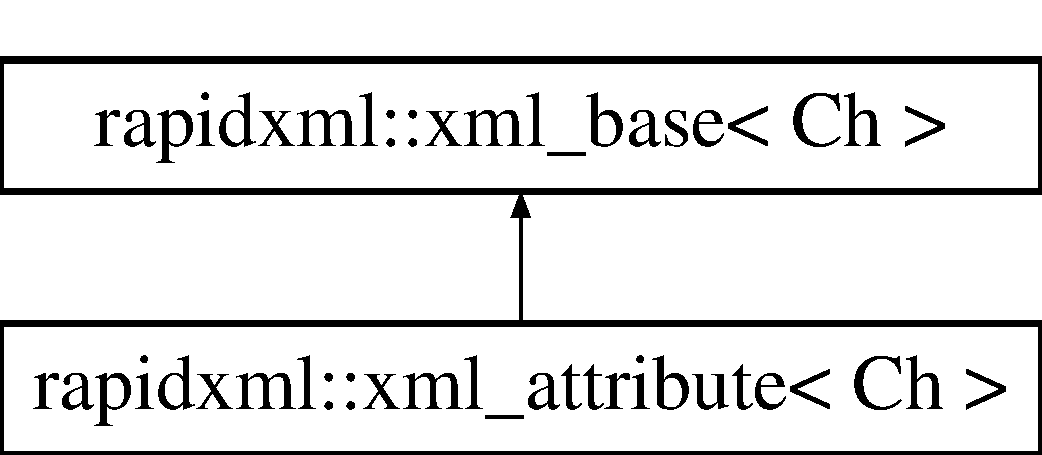
\includegraphics[height=2.000000cm]{classrapidxml_1_1xml__attribute}
\end{center}
\end{figure}
\subsection*{Public Member Functions}
\begin{DoxyCompactItemize}
\item 
\mbox{\hyperlink{classrapidxml_1_1xml__attribute_a26be291103917d3e8de110d46dd83816}{xml\+\_\+attribute}} ()
\item 
\mbox{\hyperlink{classrapidxml_1_1xml__document}{xml\+\_\+document}}$<$ Ch $>$ $\ast$ \mbox{\hyperlink{classrapidxml_1_1xml__attribute_ab0ff3bc7880a6969ddcf0bb1e0444077}{document}} () const
\item 
\mbox{\hyperlink{classrapidxml_1_1xml__attribute}{xml\+\_\+attribute}}$<$ Ch $>$ $\ast$ \mbox{\hyperlink{classrapidxml_1_1xml__attribute_abb0fb881f7247aefaec4b65b5eabc7ee}{previous\+\_\+attribute}} (const Ch $\ast$\mbox{\hyperlink{classrapidxml_1_1xml__base_aef8ae147fbee59209f714274afc80dc4}{name}}=0, std\+::size\+\_\+t \mbox{\hyperlink{classrapidxml_1_1xml__base_a20c8ffbe0c7a0b4231681ab8b99330a4}{name\+\_\+size}}=0, bool case\+\_\+sensitive=true) const
\item 
\mbox{\hyperlink{classrapidxml_1_1xml__attribute}{xml\+\_\+attribute}}$<$ Ch $>$ $\ast$ \mbox{\hyperlink{classrapidxml_1_1xml__attribute_affd0c8d0a9020df0998c507cae5474e5}{next\+\_\+attribute}} (const Ch $\ast$\mbox{\hyperlink{classrapidxml_1_1xml__base_aef8ae147fbee59209f714274afc80dc4}{name}}=0, std\+::size\+\_\+t \mbox{\hyperlink{classrapidxml_1_1xml__base_a20c8ffbe0c7a0b4231681ab8b99330a4}{name\+\_\+size}}=0, bool case\+\_\+sensitive=true) const
\end{DoxyCompactItemize}
\subsection*{Friends}
\begin{DoxyCompactItemize}
\item 
\mbox{\Hypertarget{classrapidxml_1_1xml__attribute_aa7e464ce3fe512598ff8dda47291941f}\label{classrapidxml_1_1xml__attribute_aa7e464ce3fe512598ff8dda47291941f}} 
class {\bfseries xml\+\_\+node$<$ Ch $>$}
\end{DoxyCompactItemize}
\subsection*{Additional Inherited Members}


\subsection{Detailed Description}
\subsubsection*{template$<$class Ch = char$>$\newline
class rapidxml\+::xml\+\_\+attribute$<$ Ch $>$}

Class representing attribute node of X\+ML document. Each attribute has name and value strings, which are available through \mbox{\hyperlink{classrapidxml_1_1xml__base_aef8ae147fbee59209f714274afc80dc4}{name()}} and \mbox{\hyperlink{classrapidxml_1_1xml__base_a6af65de5e59ac497cd69838f8a89d602}{value()}} functions (inherited from \mbox{\hyperlink{classrapidxml_1_1xml__base}{xml\+\_\+base}}). Note that after parse, both name and value of attribute will point to interior of source text used for parsing. Thus, this text must persist in memory for the lifetime of attribute. 
\begin{DoxyParams}{Parameters}
{\em Ch} & Character type to use. \\
\hline
\end{DoxyParams}


\subsection{Constructor \& Destructor Documentation}
\mbox{\Hypertarget{classrapidxml_1_1xml__attribute_a26be291103917d3e8de110d46dd83816}\label{classrapidxml_1_1xml__attribute_a26be291103917d3e8de110d46dd83816}} 
\index{rapidxml\+::xml\+\_\+attribute@{rapidxml\+::xml\+\_\+attribute}!xml\+\_\+attribute@{xml\+\_\+attribute}}
\index{xml\+\_\+attribute@{xml\+\_\+attribute}!rapidxml\+::xml\+\_\+attribute@{rapidxml\+::xml\+\_\+attribute}}
\subsubsection{\texorpdfstring{xml\+\_\+attribute()}{xml\_attribute()}}
{\footnotesize\ttfamily template$<$class Ch = char$>$ \\
\mbox{\hyperlink{classrapidxml_1_1xml__attribute}{rapidxml\+::xml\+\_\+attribute}}$<$ Ch $>$\+::\mbox{\hyperlink{classrapidxml_1_1xml__attribute}{xml\+\_\+attribute}} (\begin{DoxyParamCaption}{ }\end{DoxyParamCaption})\hspace{0.3cm}{\ttfamily [inline]}}

Constructs an empty attribute with the specified type. Consider using \mbox{\hyperlink{classrapidxml_1_1memory__pool}{memory\+\_\+pool}} of appropriate \mbox{\hyperlink{classrapidxml_1_1xml__document}{xml\+\_\+document}} if allocating attributes manually. 

\subsection{Member Function Documentation}
\mbox{\Hypertarget{classrapidxml_1_1xml__attribute_ab0ff3bc7880a6969ddcf0bb1e0444077}\label{classrapidxml_1_1xml__attribute_ab0ff3bc7880a6969ddcf0bb1e0444077}} 
\index{rapidxml\+::xml\+\_\+attribute@{rapidxml\+::xml\+\_\+attribute}!document@{document}}
\index{document@{document}!rapidxml\+::xml\+\_\+attribute@{rapidxml\+::xml\+\_\+attribute}}
\subsubsection{\texorpdfstring{document()}{document()}}
{\footnotesize\ttfamily template$<$class Ch = char$>$ \\
\mbox{\hyperlink{classrapidxml_1_1xml__document}{xml\+\_\+document}}$<$Ch$>$$\ast$ \mbox{\hyperlink{classrapidxml_1_1xml__attribute}{rapidxml\+::xml\+\_\+attribute}}$<$ Ch $>$\+::document (\begin{DoxyParamCaption}{ }\end{DoxyParamCaption}) const\hspace{0.3cm}{\ttfamily [inline]}}

Gets document of which attribute is a child. \begin{DoxyReturn}{Returns}
Pointer to document that contains this attribute, or 0 if there is no parent document. 
\end{DoxyReturn}
\mbox{\Hypertarget{classrapidxml_1_1xml__attribute_affd0c8d0a9020df0998c507cae5474e5}\label{classrapidxml_1_1xml__attribute_affd0c8d0a9020df0998c507cae5474e5}} 
\index{rapidxml\+::xml\+\_\+attribute@{rapidxml\+::xml\+\_\+attribute}!next\+\_\+attribute@{next\+\_\+attribute}}
\index{next\+\_\+attribute@{next\+\_\+attribute}!rapidxml\+::xml\+\_\+attribute@{rapidxml\+::xml\+\_\+attribute}}
\subsubsection{\texorpdfstring{next\+\_\+attribute()}{next\_attribute()}}
{\footnotesize\ttfamily template$<$class Ch = char$>$ \\
\mbox{\hyperlink{classrapidxml_1_1xml__attribute}{xml\+\_\+attribute}}$<$Ch$>$$\ast$ \mbox{\hyperlink{classrapidxml_1_1xml__attribute}{rapidxml\+::xml\+\_\+attribute}}$<$ Ch $>$\+::next\+\_\+attribute (\begin{DoxyParamCaption}\item[{const Ch $\ast$}]{name = {\ttfamily 0},  }\item[{std\+::size\+\_\+t}]{name\+\_\+size = {\ttfamily 0},  }\item[{bool}]{case\+\_\+sensitive = {\ttfamily true} }\end{DoxyParamCaption}) const\hspace{0.3cm}{\ttfamily [inline]}}

Gets next attribute, optionally matching attribute name. 
\begin{DoxyParams}{Parameters}
{\em name} & Name of attribute to find, or 0 to return next attribute regardless of its name; this string doesn\textquotesingle{}t have to be zero-\/terminated if name\+\_\+size is non-\/zero \\
\hline
{\em name\+\_\+size} & Size of name, in characters, or 0 to have size calculated automatically from string \\
\hline
{\em case\+\_\+sensitive} & Should name comparison be case-\/sensitive; non case-\/sensitive comparison works properly only for A\+S\+C\+II characters \\
\hline
\end{DoxyParams}
\begin{DoxyReturn}{Returns}
Pointer to found attribute, or 0 if not found. 
\end{DoxyReturn}
\mbox{\Hypertarget{classrapidxml_1_1xml__attribute_abb0fb881f7247aefaec4b65b5eabc7ee}\label{classrapidxml_1_1xml__attribute_abb0fb881f7247aefaec4b65b5eabc7ee}} 
\index{rapidxml\+::xml\+\_\+attribute@{rapidxml\+::xml\+\_\+attribute}!previous\+\_\+attribute@{previous\+\_\+attribute}}
\index{previous\+\_\+attribute@{previous\+\_\+attribute}!rapidxml\+::xml\+\_\+attribute@{rapidxml\+::xml\+\_\+attribute}}
\subsubsection{\texorpdfstring{previous\+\_\+attribute()}{previous\_attribute()}}
{\footnotesize\ttfamily template$<$class Ch = char$>$ \\
\mbox{\hyperlink{classrapidxml_1_1xml__attribute}{xml\+\_\+attribute}}$<$Ch$>$$\ast$ \mbox{\hyperlink{classrapidxml_1_1xml__attribute}{rapidxml\+::xml\+\_\+attribute}}$<$ Ch $>$\+::previous\+\_\+attribute (\begin{DoxyParamCaption}\item[{const Ch $\ast$}]{name = {\ttfamily 0},  }\item[{std\+::size\+\_\+t}]{name\+\_\+size = {\ttfamily 0},  }\item[{bool}]{case\+\_\+sensitive = {\ttfamily true} }\end{DoxyParamCaption}) const\hspace{0.3cm}{\ttfamily [inline]}}

Gets previous attribute, optionally matching attribute name. 
\begin{DoxyParams}{Parameters}
{\em name} & Name of attribute to find, or 0 to return previous attribute regardless of its name; this string doesn\textquotesingle{}t have to be zero-\/terminated if name\+\_\+size is non-\/zero \\
\hline
{\em name\+\_\+size} & Size of name, in characters, or 0 to have size calculated automatically from string \\
\hline
{\em case\+\_\+sensitive} & Should name comparison be case-\/sensitive; non case-\/sensitive comparison works properly only for A\+S\+C\+II characters \\
\hline
\end{DoxyParams}
\begin{DoxyReturn}{Returns}
Pointer to found attribute, or 0 if not found. 
\end{DoxyReturn}


The documentation for this class was generated from the following file\+:\begin{DoxyCompactItemize}
\item 
\mbox{\hyperlink{rapidxml_8hpp}{rapidxml.\+hpp}}\end{DoxyCompactItemize}

\hypertarget{classrapidxml_1_1xml__base}{}\section{rapidxml\+:\+:xml\+\_\+base$<$ Ch $>$ Class Template Reference}
\label{classrapidxml_1_1xml__base}\index{rapidxml\+::xml\+\_\+base$<$ Ch $>$@{rapidxml\+::xml\+\_\+base$<$ Ch $>$}}


{\ttfamily \#include $<$rapidxml.\+hpp$>$}

Inheritance diagram for rapidxml\+:\+:xml\+\_\+base$<$ Ch $>$\+:\begin{figure}[H]
\begin{center}
\leavevmode
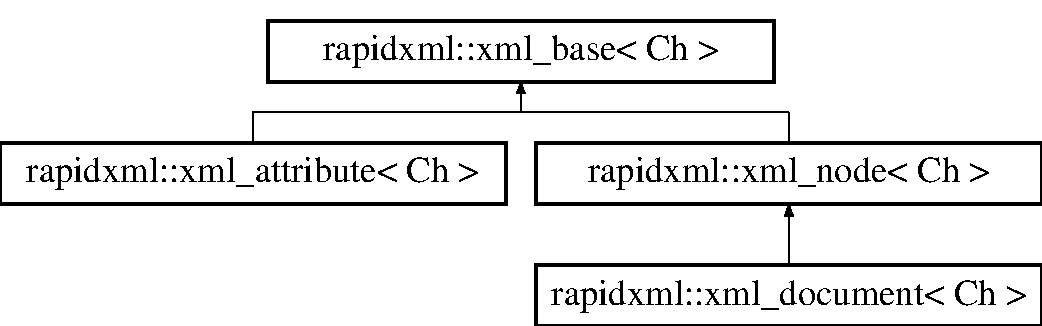
\includegraphics[height=3.000000cm]{classrapidxml_1_1xml__base}
\end{center}
\end{figure}
\subsection*{Public Member Functions}
\begin{DoxyCompactItemize}
\item 
Ch $\ast$ \mbox{\hyperlink{classrapidxml_1_1xml__base_aef8ae147fbee59209f714274afc80dc4}{name}} () const
\item 
std\+::size\+\_\+t \mbox{\hyperlink{classrapidxml_1_1xml__base_a20c8ffbe0c7a0b4231681ab8b99330a4}{name\+\_\+size}} () const
\item 
Ch $\ast$ \mbox{\hyperlink{classrapidxml_1_1xml__base_a6af65de5e59ac497cd69838f8a89d602}{value}} () const
\item 
std\+::size\+\_\+t \mbox{\hyperlink{classrapidxml_1_1xml__base_a2eb123d471b1567fa4832b6ee2b75493}{value\+\_\+size}} () const
\item 
void \mbox{\hyperlink{classrapidxml_1_1xml__base_ae55060ae958c6e6465d6c8db852ec6ce}{name}} (const Ch $\ast$name, std\+::size\+\_\+t size)
\item 
void \mbox{\hyperlink{classrapidxml_1_1xml__base_a4611ddc82ac83a527c65606600eb2a0d}{name}} (const Ch $\ast$name)
\item 
void \mbox{\hyperlink{classrapidxml_1_1xml__base_a3b183c2db7022a6d30494dd2f0ac11e9}{value}} (const Ch $\ast$value, std\+::size\+\_\+t size)
\item 
void \mbox{\hyperlink{classrapidxml_1_1xml__base_a81e63ec4bfd2d7ef0a6c2ed49be6e623}{value}} (const Ch $\ast$value)
\item 
\mbox{\hyperlink{classrapidxml_1_1xml__node}{xml\+\_\+node}}$<$ Ch $>$ $\ast$ \mbox{\hyperlink{classrapidxml_1_1xml__base_aa807062868d671a8c798d9d1bf016988}{parent}} () const
\end{DoxyCompactItemize}
\subsection*{Static Protected Member Functions}
\begin{DoxyCompactItemize}
\item 
\mbox{\Hypertarget{classrapidxml_1_1xml__base_ad96ff6b1e41dab3ff60b9bc4df769a75}\label{classrapidxml_1_1xml__base_ad96ff6b1e41dab3ff60b9bc4df769a75}} 
static Ch $\ast$ {\bfseries nullstr} ()
\end{DoxyCompactItemize}
\subsection*{Protected Attributes}
\begin{DoxyCompactItemize}
\item 
\mbox{\Hypertarget{classrapidxml_1_1xml__base_afd9851ed43e14619db0d7075ef8e9e8a}\label{classrapidxml_1_1xml__base_afd9851ed43e14619db0d7075ef8e9e8a}} 
Ch $\ast$ {\bfseries m\+\_\+name}
\item 
\mbox{\Hypertarget{classrapidxml_1_1xml__base_a278a1ea63b0b70219b946cec47fa00ea}\label{classrapidxml_1_1xml__base_a278a1ea63b0b70219b946cec47fa00ea}} 
Ch $\ast$ {\bfseries m\+\_\+value}
\item 
\mbox{\Hypertarget{classrapidxml_1_1xml__base_a5a8c76a7274b4180213796422c4df76f}\label{classrapidxml_1_1xml__base_a5a8c76a7274b4180213796422c4df76f}} 
std\+::size\+\_\+t {\bfseries m\+\_\+name\+\_\+size}
\item 
\mbox{\Hypertarget{classrapidxml_1_1xml__base_aa3a49d8ceddb8a8d7edb773a2226b89c}\label{classrapidxml_1_1xml__base_aa3a49d8ceddb8a8d7edb773a2226b89c}} 
std\+::size\+\_\+t {\bfseries m\+\_\+value\+\_\+size}
\item 
\mbox{\Hypertarget{classrapidxml_1_1xml__base_a90d5f660f078f66563fd7b2d8387ccb0}\label{classrapidxml_1_1xml__base_a90d5f660f078f66563fd7b2d8387ccb0}} 
\mbox{\hyperlink{classrapidxml_1_1xml__node}{xml\+\_\+node}}$<$ Ch $>$ $\ast$ {\bfseries m\+\_\+parent}
\end{DoxyCompactItemize}


\subsection{Detailed Description}
\subsubsection*{template$<$class Ch = char$>$\newline
class rapidxml\+::xml\+\_\+base$<$ Ch $>$}

Base class for \mbox{\hyperlink{classrapidxml_1_1xml__node}{xml\+\_\+node}} and \mbox{\hyperlink{classrapidxml_1_1xml__attribute}{xml\+\_\+attribute}} implementing common functions\+: \mbox{\hyperlink{classrapidxml_1_1xml__base_aef8ae147fbee59209f714274afc80dc4}{name()}}, \mbox{\hyperlink{classrapidxml_1_1xml__base_a20c8ffbe0c7a0b4231681ab8b99330a4}{name\+\_\+size()}}, \mbox{\hyperlink{classrapidxml_1_1xml__base_a6af65de5e59ac497cd69838f8a89d602}{value()}}, \mbox{\hyperlink{classrapidxml_1_1xml__base_a2eb123d471b1567fa4832b6ee2b75493}{value\+\_\+size()}} and \mbox{\hyperlink{classrapidxml_1_1xml__base_aa807062868d671a8c798d9d1bf016988}{parent()}}. 
\begin{DoxyParams}{Parameters}
{\em Ch} & Character type to use \\
\hline
\end{DoxyParams}


\subsection{Member Function Documentation}
\mbox{\Hypertarget{classrapidxml_1_1xml__base_aef8ae147fbee59209f714274afc80dc4}\label{classrapidxml_1_1xml__base_aef8ae147fbee59209f714274afc80dc4}} 
\index{rapidxml\+::xml\+\_\+base@{rapidxml\+::xml\+\_\+base}!name@{name}}
\index{name@{name}!rapidxml\+::xml\+\_\+base@{rapidxml\+::xml\+\_\+base}}
\subsubsection{\texorpdfstring{name()}{name()}\hspace{0.1cm}{\footnotesize\ttfamily [1/3]}}
{\footnotesize\ttfamily template$<$class Ch  = char$>$ \\
Ch$\ast$ \mbox{\hyperlink{classrapidxml_1_1xml__base}{rapidxml\+::xml\+\_\+base}}$<$ Ch $>$\+::name (\begin{DoxyParamCaption}{ }\end{DoxyParamCaption}) const\hspace{0.3cm}{\ttfamily [inline]}}

Gets name of the node. Interpretation of name depends on type of node. Note that name will not be zero-\/terminated if rapidxml\+::parse\+\_\+no\+\_\+string\+\_\+terminators option was selected during parse. ~\newline
~\newline
 Use \mbox{\hyperlink{classrapidxml_1_1xml__base_a20c8ffbe0c7a0b4231681ab8b99330a4}{name\+\_\+size()}} function to determine length of the name. \begin{DoxyReturn}{Returns}
Name of node, or empty string if node has no name. 
\end{DoxyReturn}
\mbox{\Hypertarget{classrapidxml_1_1xml__base_ae55060ae958c6e6465d6c8db852ec6ce}\label{classrapidxml_1_1xml__base_ae55060ae958c6e6465d6c8db852ec6ce}} 
\index{rapidxml\+::xml\+\_\+base@{rapidxml\+::xml\+\_\+base}!name@{name}}
\index{name@{name}!rapidxml\+::xml\+\_\+base@{rapidxml\+::xml\+\_\+base}}
\subsubsection{\texorpdfstring{name()}{name()}\hspace{0.1cm}{\footnotesize\ttfamily [2/3]}}
{\footnotesize\ttfamily template$<$class Ch  = char$>$ \\
void \mbox{\hyperlink{classrapidxml_1_1xml__base}{rapidxml\+::xml\+\_\+base}}$<$ Ch $>$\+::name (\begin{DoxyParamCaption}\item[{const Ch $\ast$}]{name,  }\item[{std\+::size\+\_\+t}]{size }\end{DoxyParamCaption})\hspace{0.3cm}{\ttfamily [inline]}}

Sets name of node to a non zero-\/terminated string. See ownership\+\_\+of\+\_\+strings. ~\newline
~\newline
 Note that node does not own its name or value, it only stores a pointer to it. It will not delete or otherwise free the pointer on destruction. It is reponsibility of the user to properly manage lifetime of the string. The easiest way to achieve it is to use \mbox{\hyperlink{classrapidxml_1_1memory__pool}{memory\+\_\+pool}} of the document to allocate the string -\/ on destruction of the document the string will be automatically freed. ~\newline
~\newline
 Size of name must be specified separately, because name does not have to be zero terminated. Use \mbox{\hyperlink{classrapidxml_1_1xml__base_a4611ddc82ac83a527c65606600eb2a0d}{name(const Ch $\ast$)}} function to have the length automatically calculated (string must be zero terminated). 
\begin{DoxyParams}{Parameters}
{\em name} & Name of node to set. Does not have to be zero terminated. \\
\hline
{\em size} & Size of name, in characters. This does not include zero terminator, if one is present. \\
\hline
\end{DoxyParams}
\mbox{\Hypertarget{classrapidxml_1_1xml__base_a4611ddc82ac83a527c65606600eb2a0d}\label{classrapidxml_1_1xml__base_a4611ddc82ac83a527c65606600eb2a0d}} 
\index{rapidxml\+::xml\+\_\+base@{rapidxml\+::xml\+\_\+base}!name@{name}}
\index{name@{name}!rapidxml\+::xml\+\_\+base@{rapidxml\+::xml\+\_\+base}}
\subsubsection{\texorpdfstring{name()}{name()}\hspace{0.1cm}{\footnotesize\ttfamily [3/3]}}
{\footnotesize\ttfamily template$<$class Ch  = char$>$ \\
void \mbox{\hyperlink{classrapidxml_1_1xml__base}{rapidxml\+::xml\+\_\+base}}$<$ Ch $>$\+::name (\begin{DoxyParamCaption}\item[{const Ch $\ast$}]{name }\end{DoxyParamCaption})\hspace{0.3cm}{\ttfamily [inline]}}

Sets name of node to a zero-\/terminated string. See also ownership\+\_\+of\+\_\+strings and \mbox{\hyperlink{classrapidxml_1_1xml__base_ae55060ae958c6e6465d6c8db852ec6ce}{xml\+\_\+node\+::name(const Ch $\ast$, std\+::size\+\_\+t)}}. 
\begin{DoxyParams}{Parameters}
{\em name} & Name of node to set. Must be zero terminated. \\
\hline
\end{DoxyParams}
\mbox{\Hypertarget{classrapidxml_1_1xml__base_a20c8ffbe0c7a0b4231681ab8b99330a4}\label{classrapidxml_1_1xml__base_a20c8ffbe0c7a0b4231681ab8b99330a4}} 
\index{rapidxml\+::xml\+\_\+base@{rapidxml\+::xml\+\_\+base}!name\+\_\+size@{name\+\_\+size}}
\index{name\+\_\+size@{name\+\_\+size}!rapidxml\+::xml\+\_\+base@{rapidxml\+::xml\+\_\+base}}
\subsubsection{\texorpdfstring{name\+\_\+size()}{name\_size()}}
{\footnotesize\ttfamily template$<$class Ch  = char$>$ \\
std\+::size\+\_\+t \mbox{\hyperlink{classrapidxml_1_1xml__base}{rapidxml\+::xml\+\_\+base}}$<$ Ch $>$\+::name\+\_\+size (\begin{DoxyParamCaption}{ }\end{DoxyParamCaption}) const\hspace{0.3cm}{\ttfamily [inline]}}

Gets size of node name, not including terminator character. This function works correctly irrespective of whether name is or is not zero terminated. \begin{DoxyReturn}{Returns}
Size of node name, in characters. 
\end{DoxyReturn}
\mbox{\Hypertarget{classrapidxml_1_1xml__base_aa807062868d671a8c798d9d1bf016988}\label{classrapidxml_1_1xml__base_aa807062868d671a8c798d9d1bf016988}} 
\index{rapidxml\+::xml\+\_\+base@{rapidxml\+::xml\+\_\+base}!parent@{parent}}
\index{parent@{parent}!rapidxml\+::xml\+\_\+base@{rapidxml\+::xml\+\_\+base}}
\subsubsection{\texorpdfstring{parent()}{parent()}}
{\footnotesize\ttfamily template$<$class Ch  = char$>$ \\
\mbox{\hyperlink{classrapidxml_1_1xml__node}{xml\+\_\+node}}$<$Ch$>$$\ast$ \mbox{\hyperlink{classrapidxml_1_1xml__base}{rapidxml\+::xml\+\_\+base}}$<$ Ch $>$\+::parent (\begin{DoxyParamCaption}{ }\end{DoxyParamCaption}) const\hspace{0.3cm}{\ttfamily [inline]}}

Gets node parent. \begin{DoxyReturn}{Returns}
Pointer to parent node, or 0 if there is no parent. 
\end{DoxyReturn}
\mbox{\Hypertarget{classrapidxml_1_1xml__base_a6af65de5e59ac497cd69838f8a89d602}\label{classrapidxml_1_1xml__base_a6af65de5e59ac497cd69838f8a89d602}} 
\index{rapidxml\+::xml\+\_\+base@{rapidxml\+::xml\+\_\+base}!value@{value}}
\index{value@{value}!rapidxml\+::xml\+\_\+base@{rapidxml\+::xml\+\_\+base}}
\subsubsection{\texorpdfstring{value()}{value()}\hspace{0.1cm}{\footnotesize\ttfamily [1/3]}}
{\footnotesize\ttfamily template$<$class Ch  = char$>$ \\
Ch$\ast$ \mbox{\hyperlink{classrapidxml_1_1xml__base}{rapidxml\+::xml\+\_\+base}}$<$ Ch $>$\+::value (\begin{DoxyParamCaption}{ }\end{DoxyParamCaption}) const\hspace{0.3cm}{\ttfamily [inline]}}

Gets value of node. Interpretation of value depends on type of node. Note that value will not be zero-\/terminated if rapidxml\+::parse\+\_\+no\+\_\+string\+\_\+terminators option was selected during parse. ~\newline
~\newline
 Use \mbox{\hyperlink{classrapidxml_1_1xml__base_a2eb123d471b1567fa4832b6ee2b75493}{value\+\_\+size()}} function to determine length of the value. \begin{DoxyReturn}{Returns}
Value of node, or empty string if node has no value. 
\end{DoxyReturn}
\mbox{\Hypertarget{classrapidxml_1_1xml__base_a3b183c2db7022a6d30494dd2f0ac11e9}\label{classrapidxml_1_1xml__base_a3b183c2db7022a6d30494dd2f0ac11e9}} 
\index{rapidxml\+::xml\+\_\+base@{rapidxml\+::xml\+\_\+base}!value@{value}}
\index{value@{value}!rapidxml\+::xml\+\_\+base@{rapidxml\+::xml\+\_\+base}}
\subsubsection{\texorpdfstring{value()}{value()}\hspace{0.1cm}{\footnotesize\ttfamily [2/3]}}
{\footnotesize\ttfamily template$<$class Ch  = char$>$ \\
void \mbox{\hyperlink{classrapidxml_1_1xml__base}{rapidxml\+::xml\+\_\+base}}$<$ Ch $>$\+::value (\begin{DoxyParamCaption}\item[{const Ch $\ast$}]{value,  }\item[{std\+::size\+\_\+t}]{size }\end{DoxyParamCaption})\hspace{0.3cm}{\ttfamily [inline]}}

Sets value of node to a non zero-\/terminated string. See ownership\+\_\+of\+\_\+strings. ~\newline
~\newline
 Note that node does not own its name or value, it only stores a pointer to it. It will not delete or otherwise free the pointer on destruction. It is reponsibility of the user to properly manage lifetime of the string. The easiest way to achieve it is to use \mbox{\hyperlink{classrapidxml_1_1memory__pool}{memory\+\_\+pool}} of the document to allocate the string -\/ on destruction of the document the string will be automatically freed. ~\newline
~\newline
 Size of value must be specified separately, because it does not have to be zero terminated. Use \mbox{\hyperlink{classrapidxml_1_1xml__base_a81e63ec4bfd2d7ef0a6c2ed49be6e623}{value(const Ch $\ast$)}} function to have the length automatically calculated (string must be zero terminated). ~\newline
~\newline
 If an element has a child node of type node\+\_\+data, it will take precedence over element value when printing. If you want to manipulate data of elements using values, use parser flag rapidxml\+::parse\+\_\+no\+\_\+data\+\_\+nodes to prevent creation of data nodes by the parser. 
\begin{DoxyParams}{Parameters}
{\em value} & value of node to set. Does not have to be zero terminated. \\
\hline
{\em size} & Size of value, in characters. This does not include zero terminator, if one is present. \\
\hline
\end{DoxyParams}
\mbox{\Hypertarget{classrapidxml_1_1xml__base_a81e63ec4bfd2d7ef0a6c2ed49be6e623}\label{classrapidxml_1_1xml__base_a81e63ec4bfd2d7ef0a6c2ed49be6e623}} 
\index{rapidxml\+::xml\+\_\+base@{rapidxml\+::xml\+\_\+base}!value@{value}}
\index{value@{value}!rapidxml\+::xml\+\_\+base@{rapidxml\+::xml\+\_\+base}}
\subsubsection{\texorpdfstring{value()}{value()}\hspace{0.1cm}{\footnotesize\ttfamily [3/3]}}
{\footnotesize\ttfamily template$<$class Ch  = char$>$ \\
void \mbox{\hyperlink{classrapidxml_1_1xml__base}{rapidxml\+::xml\+\_\+base}}$<$ Ch $>$\+::value (\begin{DoxyParamCaption}\item[{const Ch $\ast$}]{value }\end{DoxyParamCaption})\hspace{0.3cm}{\ttfamily [inline]}}

Sets value of node to a zero-\/terminated string. See also ownership\+\_\+of\+\_\+strings and \mbox{\hyperlink{classrapidxml_1_1xml__base_a3b183c2db7022a6d30494dd2f0ac11e9}{xml\+\_\+node\+::value(const Ch $\ast$, std\+::size\+\_\+t)}}. 
\begin{DoxyParams}{Parameters}
{\em value} & Vame of node to set. Must be zero terminated. \\
\hline
\end{DoxyParams}
\mbox{\Hypertarget{classrapidxml_1_1xml__base_a2eb123d471b1567fa4832b6ee2b75493}\label{classrapidxml_1_1xml__base_a2eb123d471b1567fa4832b6ee2b75493}} 
\index{rapidxml\+::xml\+\_\+base@{rapidxml\+::xml\+\_\+base}!value\+\_\+size@{value\+\_\+size}}
\index{value\+\_\+size@{value\+\_\+size}!rapidxml\+::xml\+\_\+base@{rapidxml\+::xml\+\_\+base}}
\subsubsection{\texorpdfstring{value\+\_\+size()}{value\_size()}}
{\footnotesize\ttfamily template$<$class Ch  = char$>$ \\
std\+::size\+\_\+t \mbox{\hyperlink{classrapidxml_1_1xml__base}{rapidxml\+::xml\+\_\+base}}$<$ Ch $>$\+::value\+\_\+size (\begin{DoxyParamCaption}{ }\end{DoxyParamCaption}) const\hspace{0.3cm}{\ttfamily [inline]}}

Gets size of node value, not including terminator character. This function works correctly irrespective of whether value is or is not zero terminated. \begin{DoxyReturn}{Returns}
Size of node value, in characters. 
\end{DoxyReturn}


The documentation for this class was generated from the following file\+:\begin{DoxyCompactItemize}
\item 
\mbox{\hyperlink{rapidxml_8hpp}{rapidxml.\+hpp}}\end{DoxyCompactItemize}

\hypertarget{classrapidxml_1_1xml__document}{}\section{rapidxml\+:\+:xml\+\_\+document$<$ Ch $>$ Class Template Reference}
\label{classrapidxml_1_1xml__document}\index{rapidxml\+::xml\+\_\+document$<$ Ch $>$@{rapidxml\+::xml\+\_\+document$<$ Ch $>$}}


{\ttfamily \#include $<$rapidxml.\+hpp$>$}

Inheritance diagram for rapidxml\+:\+:xml\+\_\+document$<$ Ch $>$\+:\begin{figure}[H]
\begin{center}
\leavevmode
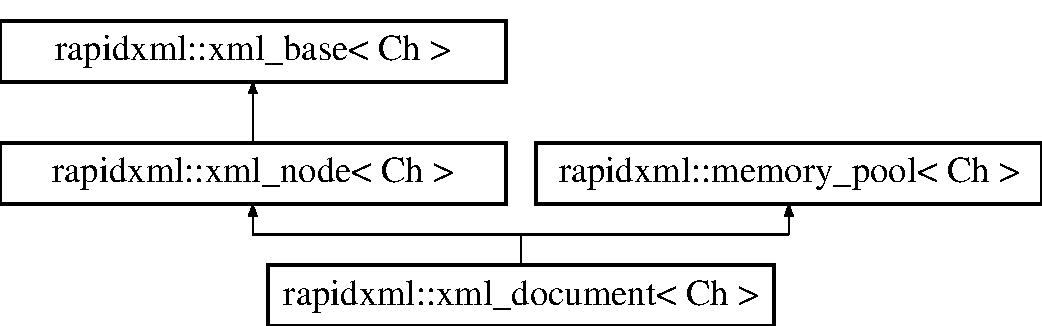
\includegraphics[height=3.000000cm]{classrapidxml_1_1xml__document}
\end{center}
\end{figure}
\subsection*{Public Member Functions}
\begin{DoxyCompactItemize}
\item 
\mbox{\Hypertarget{classrapidxml_1_1xml__document_aae8841b15085ba8f32ff46587ace28f5}\label{classrapidxml_1_1xml__document_aae8841b15085ba8f32ff46587ace28f5}} 
\mbox{\hyperlink{classrapidxml_1_1xml__document_aae8841b15085ba8f32ff46587ace28f5}{xml\+\_\+document}} ()
\begin{DoxyCompactList}\small\item\em Constructs empty X\+ML document. \end{DoxyCompactList}\item 
{\footnotesize template$<$int Flags$>$ }\\void \mbox{\hyperlink{classrapidxml_1_1xml__document_ac6e73ff9ac323bf5a370c38feb03a6b1}{parse}} (Ch $\ast$text)
\item 
void \mbox{\hyperlink{classrapidxml_1_1xml__document_a826929ff54242532198701f19ff5f83f}{clear}} ()
\end{DoxyCompactItemize}
\subsection*{Additional Inherited Members}


\subsection{Detailed Description}
\subsubsection*{template$<$class Ch = char$>$\newline
class rapidxml\+::xml\+\_\+document$<$ Ch $>$}

This class represents root of the D\+OM hierarchy. It is also an \mbox{\hyperlink{classrapidxml_1_1xml__node}{xml\+\_\+node}} and a \mbox{\hyperlink{classrapidxml_1_1memory__pool}{memory\+\_\+pool}} through public inheritance. Use \mbox{\hyperlink{classrapidxml_1_1xml__document_ac6e73ff9ac323bf5a370c38feb03a6b1}{parse()}} function to build a D\+OM tree from a zero-\/terminated X\+ML text string. \mbox{\hyperlink{classrapidxml_1_1xml__document_ac6e73ff9ac323bf5a370c38feb03a6b1}{parse()}} function allocates memory for nodes and attributes by using functions of \mbox{\hyperlink{classrapidxml_1_1xml__document}{xml\+\_\+document}}, which are inherited from \mbox{\hyperlink{classrapidxml_1_1memory__pool}{memory\+\_\+pool}}. To access root node of the document, use the document itself, as if it was an \mbox{\hyperlink{classrapidxml_1_1xml__node}{xml\+\_\+node}}. 
\begin{DoxyParams}{Parameters}
{\em Ch} & Character type to use. \\
\hline
\end{DoxyParams}


\subsection{Member Function Documentation}
\mbox{\Hypertarget{classrapidxml_1_1xml__document_a826929ff54242532198701f19ff5f83f}\label{classrapidxml_1_1xml__document_a826929ff54242532198701f19ff5f83f}} 
\index{rapidxml\+::xml\+\_\+document@{rapidxml\+::xml\+\_\+document}!clear@{clear}}
\index{clear@{clear}!rapidxml\+::xml\+\_\+document@{rapidxml\+::xml\+\_\+document}}
\subsubsection{\texorpdfstring{clear()}{clear()}}
{\footnotesize\ttfamily template$<$class Ch  = char$>$ \\
void \mbox{\hyperlink{classrapidxml_1_1xml__document}{rapidxml\+::xml\+\_\+document}}$<$ Ch $>$\+::clear (\begin{DoxyParamCaption}{ }\end{DoxyParamCaption})\hspace{0.3cm}{\ttfamily [inline]}}

Clears the document by deleting all nodes and clearing the memory pool. All nodes owned by document pool are destroyed. \mbox{\Hypertarget{classrapidxml_1_1xml__document_ac6e73ff9ac323bf5a370c38feb03a6b1}\label{classrapidxml_1_1xml__document_ac6e73ff9ac323bf5a370c38feb03a6b1}} 
\index{rapidxml\+::xml\+\_\+document@{rapidxml\+::xml\+\_\+document}!parse@{parse}}
\index{parse@{parse}!rapidxml\+::xml\+\_\+document@{rapidxml\+::xml\+\_\+document}}
\subsubsection{\texorpdfstring{parse()}{parse()}}
{\footnotesize\ttfamily template$<$class Ch  = char$>$ \\
template$<$int Flags$>$ \\
void \mbox{\hyperlink{classrapidxml_1_1xml__document}{rapidxml\+::xml\+\_\+document}}$<$ Ch $>$\+::parse (\begin{DoxyParamCaption}\item[{Ch $\ast$}]{text }\end{DoxyParamCaption})\hspace{0.3cm}{\ttfamily [inline]}}

Parses zero-\/terminated X\+ML string according to given flags. Passed string will be modified by the parser, unless rapidxml\+::parse\+\_\+non\+\_\+destructive flag is used. The string must persist for the lifetime of the document. In case of error, \mbox{\hyperlink{classrapidxml_1_1parse__error}{rapidxml\+::parse\+\_\+error}} exception will be thrown. ~\newline
~\newline
 If you want to parse contents of a file, you must first load the file into the memory, and pass pointer to its beginning. Make sure that data is zero-\/terminated. ~\newline
~\newline
 Document can be parsed into multiple times. Each new call to parse removes previous nodes and attributes (if any), but does not clear memory pool. 
\begin{DoxyParams}{Parameters}
{\em text} & X\+ML data to parse; pointer is non-\/const to denote fact that this data may be modified by the parser. \\
\hline
\end{DoxyParams}


The documentation for this class was generated from the following file\+:\begin{DoxyCompactItemize}
\item 
\mbox{\hyperlink{rapidxml_8hpp}{rapidxml.\+hpp}}\end{DoxyCompactItemize}

\hypertarget{classrapidxml_1_1xml__node}{}\section{rapidxml\+:\+:xml\+\_\+node$<$ Ch $>$ Class Template Reference}
\label{classrapidxml_1_1xml__node}\index{rapidxml\+::xml\+\_\+node$<$ Ch $>$@{rapidxml\+::xml\+\_\+node$<$ Ch $>$}}


{\ttfamily \#include $<$rapidxml.\+hpp$>$}

Inheritance diagram for rapidxml\+:\+:xml\+\_\+node$<$ Ch $>$\+:\begin{figure}[H]
\begin{center}
\leavevmode
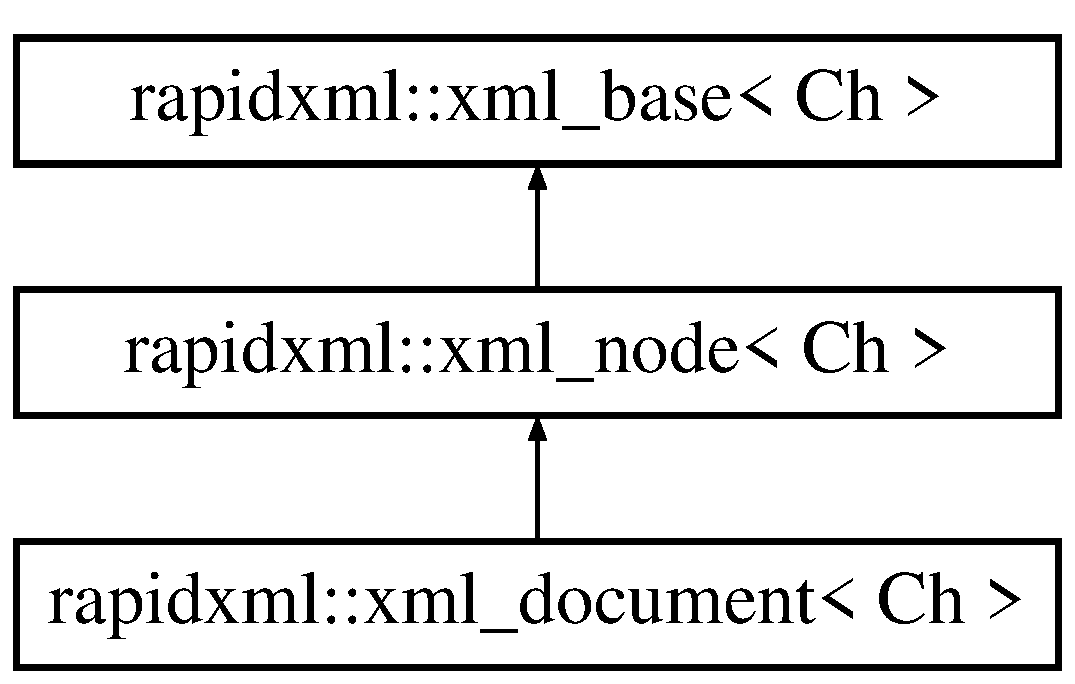
\includegraphics[height=3.000000cm]{classrapidxml_1_1xml__node}
\end{center}
\end{figure}
\subsection*{Public Member Functions}
\begin{DoxyCompactItemize}
\item 
\mbox{\hyperlink{classrapidxml_1_1xml__node_a8bd9019960b90605a45998b661fb1b0e}{xml\+\_\+node}} (\mbox{\hyperlink{rapidxml_8hpp_abb456db38f7efb746c4330eed6072a7c}{node\+\_\+type}} \mbox{\hyperlink{classrapidxml_1_1xml__node_a5f91729128856b0aaab598d4364ace60}{type}})
\item 
\mbox{\hyperlink{rapidxml_8hpp_abb456db38f7efb746c4330eed6072a7c}{node\+\_\+type}} \mbox{\hyperlink{classrapidxml_1_1xml__node_a5f91729128856b0aaab598d4364ace60}{type}} () const
\item 
\mbox{\hyperlink{classrapidxml_1_1xml__document}{xml\+\_\+document}}$<$ Ch $>$ $\ast$ \mbox{\hyperlink{classrapidxml_1_1xml__node_af23d2d56182411e9261ca6974bfd767f}{document}} () const
\item 
\mbox{\hyperlink{classrapidxml_1_1xml__node}{xml\+\_\+node}}$<$ Ch $>$ $\ast$ \mbox{\hyperlink{classrapidxml_1_1xml__node_acdf3691224d683f50692616a92a75d3f}{first\+\_\+node}} (const Ch $\ast$\mbox{\hyperlink{classrapidxml_1_1xml__base_aef8ae147fbee59209f714274afc80dc4}{name}}=0, std\+::size\+\_\+t \mbox{\hyperlink{classrapidxml_1_1xml__base_a20c8ffbe0c7a0b4231681ab8b99330a4}{name\+\_\+size}}=0, bool case\+\_\+sensitive=true) const
\item 
\mbox{\hyperlink{classrapidxml_1_1xml__node}{xml\+\_\+node}}$<$ Ch $>$ $\ast$ \mbox{\hyperlink{classrapidxml_1_1xml__node_a524d427e32c72fba9de1857e02e82fa7}{last\+\_\+node}} (const Ch $\ast$\mbox{\hyperlink{classrapidxml_1_1xml__base_aef8ae147fbee59209f714274afc80dc4}{name}}=0, std\+::size\+\_\+t \mbox{\hyperlink{classrapidxml_1_1xml__base_a20c8ffbe0c7a0b4231681ab8b99330a4}{name\+\_\+size}}=0, bool case\+\_\+sensitive=true) const
\item 
\mbox{\hyperlink{classrapidxml_1_1xml__node}{xml\+\_\+node}}$<$ Ch $>$ $\ast$ \mbox{\hyperlink{classrapidxml_1_1xml__node_aebcc42042ded78fb7020e2783f7d5426}{previous\+\_\+sibling}} (const Ch $\ast$\mbox{\hyperlink{classrapidxml_1_1xml__base_aef8ae147fbee59209f714274afc80dc4}{name}}=0, std\+::size\+\_\+t \mbox{\hyperlink{classrapidxml_1_1xml__base_a20c8ffbe0c7a0b4231681ab8b99330a4}{name\+\_\+size}}=0, bool case\+\_\+sensitive=true) const
\item 
\mbox{\hyperlink{classrapidxml_1_1xml__node}{xml\+\_\+node}}$<$ Ch $>$ $\ast$ \mbox{\hyperlink{classrapidxml_1_1xml__node_ad36aa4445ced578f93c3e06770cb3ef9}{next\+\_\+sibling}} (const Ch $\ast$\mbox{\hyperlink{classrapidxml_1_1xml__base_aef8ae147fbee59209f714274afc80dc4}{name}}=0, std\+::size\+\_\+t \mbox{\hyperlink{classrapidxml_1_1xml__base_a20c8ffbe0c7a0b4231681ab8b99330a4}{name\+\_\+size}}=0, bool case\+\_\+sensitive=true) const
\item 
\mbox{\hyperlink{classrapidxml_1_1xml__attribute}{xml\+\_\+attribute}}$<$ Ch $>$ $\ast$ \mbox{\hyperlink{classrapidxml_1_1xml__node_ab816ab6f13ee4b0588d5b76b0697511c}{first\+\_\+attribute}} (const Ch $\ast$\mbox{\hyperlink{classrapidxml_1_1xml__base_aef8ae147fbee59209f714274afc80dc4}{name}}=0, std\+::size\+\_\+t \mbox{\hyperlink{classrapidxml_1_1xml__base_a20c8ffbe0c7a0b4231681ab8b99330a4}{name\+\_\+size}}=0, bool case\+\_\+sensitive=true) const
\item 
\mbox{\hyperlink{classrapidxml_1_1xml__attribute}{xml\+\_\+attribute}}$<$ Ch $>$ $\ast$ \mbox{\hyperlink{classrapidxml_1_1xml__node_a67db03d1568dc6891573210ddba61520}{last\+\_\+attribute}} (const Ch $\ast$\mbox{\hyperlink{classrapidxml_1_1xml__base_aef8ae147fbee59209f714274afc80dc4}{name}}=0, std\+::size\+\_\+t \mbox{\hyperlink{classrapidxml_1_1xml__base_a20c8ffbe0c7a0b4231681ab8b99330a4}{name\+\_\+size}}=0, bool case\+\_\+sensitive=true) const
\item 
void \mbox{\hyperlink{classrapidxml_1_1xml__node_a499bbc9300c1b06821d5c08b24164c68}{type}} (\mbox{\hyperlink{rapidxml_8hpp_abb456db38f7efb746c4330eed6072a7c}{node\+\_\+type}} type)
\item 
void \mbox{\hyperlink{classrapidxml_1_1xml__node_ae86e92908c3eab40bbed8216e4f3f3cb}{prepend\+\_\+node}} (\mbox{\hyperlink{classrapidxml_1_1xml__node}{xml\+\_\+node}}$<$ Ch $>$ $\ast$child)
\item 
void \mbox{\hyperlink{classrapidxml_1_1xml__node_a8696d098ecc9c4d2a646b43e91d58e31}{append\+\_\+node}} (\mbox{\hyperlink{classrapidxml_1_1xml__node}{xml\+\_\+node}}$<$ Ch $>$ $\ast$child)
\item 
void \mbox{\hyperlink{classrapidxml_1_1xml__node_a666880f42a7e486d78cc45ed51c7c46d}{insert\+\_\+node}} (\mbox{\hyperlink{classrapidxml_1_1xml__node}{xml\+\_\+node}}$<$ Ch $>$ $\ast$where, \mbox{\hyperlink{classrapidxml_1_1xml__node}{xml\+\_\+node}}$<$ Ch $>$ $\ast$child)
\item 
void \mbox{\hyperlink{classrapidxml_1_1xml__node_a62bf7b276cf7a651a3337f5e0a0ef6ac}{remove\+\_\+first\+\_\+node}} ()
\item 
void \mbox{\hyperlink{classrapidxml_1_1xml__node_a9182512e948ec451a83f116cce7c7674}{remove\+\_\+last\+\_\+node}} ()
\item 
\mbox{\Hypertarget{classrapidxml_1_1xml__node_a98289923eb9e8889418a9eb0207ea35c}\label{classrapidxml_1_1xml__node_a98289923eb9e8889418a9eb0207ea35c}} 
void \mbox{\hyperlink{classrapidxml_1_1xml__node_a98289923eb9e8889418a9eb0207ea35c}{remove\+\_\+node}} (\mbox{\hyperlink{classrapidxml_1_1xml__node}{xml\+\_\+node}}$<$ Ch $>$ $\ast$where)
\begin{DoxyCompactList}\small\item\em Removes specified child from the node. \end{DoxyCompactList}\item 
\mbox{\Hypertarget{classrapidxml_1_1xml__node_a95735358b079ae0adcfbbac69aa1fbc3}\label{classrapidxml_1_1xml__node_a95735358b079ae0adcfbbac69aa1fbc3}} 
void \mbox{\hyperlink{classrapidxml_1_1xml__node_a95735358b079ae0adcfbbac69aa1fbc3}{remove\+\_\+all\+\_\+nodes}} ()
\begin{DoxyCompactList}\small\item\em Removes all child nodes (but not attributes). \end{DoxyCompactList}\item 
void \mbox{\hyperlink{classrapidxml_1_1xml__node_a8b62ee76489faf8e2d1210869d547684}{prepend\+\_\+attribute}} (\mbox{\hyperlink{classrapidxml_1_1xml__attribute}{xml\+\_\+attribute}}$<$ Ch $>$ $\ast$attribute)
\item 
void \mbox{\hyperlink{classrapidxml_1_1xml__node_a33ce3386f8c42dd4db658b75cbb6e6c4}{append\+\_\+attribute}} (\mbox{\hyperlink{classrapidxml_1_1xml__attribute}{xml\+\_\+attribute}}$<$ Ch $>$ $\ast$attribute)
\item 
void \mbox{\hyperlink{classrapidxml_1_1xml__node_a9fe659cdf4a5b3bbf5e8ffc98db5a84f}{insert\+\_\+attribute}} (\mbox{\hyperlink{classrapidxml_1_1xml__attribute}{xml\+\_\+attribute}}$<$ Ch $>$ $\ast$where, \mbox{\hyperlink{classrapidxml_1_1xml__attribute}{xml\+\_\+attribute}}$<$ Ch $>$ $\ast$attribute)
\item 
void \mbox{\hyperlink{classrapidxml_1_1xml__node_aa95192d2a165cca16c551ed2a2a06aec}{remove\+\_\+first\+\_\+attribute}} ()
\item 
void \mbox{\hyperlink{classrapidxml_1_1xml__node_a1781a2cbedc9a51d609ad5b528125635}{remove\+\_\+last\+\_\+attribute}} ()
\item 
void \mbox{\hyperlink{classrapidxml_1_1xml__node_a6f97b1b4f46a94a4587915df3c0c6b57}{remove\+\_\+attribute}} (\mbox{\hyperlink{classrapidxml_1_1xml__attribute}{xml\+\_\+attribute}}$<$ Ch $>$ $\ast$where)
\item 
\mbox{\Hypertarget{classrapidxml_1_1xml__node_aa8d5d9484aa1eb5ff1841a073c84c1aa}\label{classrapidxml_1_1xml__node_aa8d5d9484aa1eb5ff1841a073c84c1aa}} 
void \mbox{\hyperlink{classrapidxml_1_1xml__node_aa8d5d9484aa1eb5ff1841a073c84c1aa}{remove\+\_\+all\+\_\+attributes}} ()
\begin{DoxyCompactList}\small\item\em Removes all attributes of node. \end{DoxyCompactList}\end{DoxyCompactItemize}
\subsection*{Additional Inherited Members}


\subsection{Detailed Description}
\subsubsection*{template$<$class Ch = char$>$\newline
class rapidxml\+::xml\+\_\+node$<$ Ch $>$}

Class representing a node of X\+ML document. Each node may have associated name and value strings, which are available through \mbox{\hyperlink{classrapidxml_1_1xml__base_aef8ae147fbee59209f714274afc80dc4}{name()}} and \mbox{\hyperlink{classrapidxml_1_1xml__base_a6af65de5e59ac497cd69838f8a89d602}{value()}} functions. Interpretation of name and value depends on type of the node. Type of node can be determined by using \mbox{\hyperlink{classrapidxml_1_1xml__node_a5f91729128856b0aaab598d4364ace60}{type()}} function. ~\newline
~\newline
 Note that after parse, both name and value of node, if any, will point interior of source text used for parsing. Thus, this text must persist in the memory for the lifetime of node. 
\begin{DoxyParams}{Parameters}
{\em Ch} & Character type to use. \\
\hline
\end{DoxyParams}


\subsection{Constructor \& Destructor Documentation}
\mbox{\Hypertarget{classrapidxml_1_1xml__node_a8bd9019960b90605a45998b661fb1b0e}\label{classrapidxml_1_1xml__node_a8bd9019960b90605a45998b661fb1b0e}} 
\index{rapidxml\+::xml\+\_\+node@{rapidxml\+::xml\+\_\+node}!xml\+\_\+node@{xml\+\_\+node}}
\index{xml\+\_\+node@{xml\+\_\+node}!rapidxml\+::xml\+\_\+node@{rapidxml\+::xml\+\_\+node}}
\subsubsection{\texorpdfstring{xml\+\_\+node()}{xml\_node()}}
{\footnotesize\ttfamily template$<$class Ch = char$>$ \\
\mbox{\hyperlink{classrapidxml_1_1xml__node}{rapidxml\+::xml\+\_\+node}}$<$ Ch $>$\+::\mbox{\hyperlink{classrapidxml_1_1xml__node}{xml\+\_\+node}} (\begin{DoxyParamCaption}\item[{\mbox{\hyperlink{rapidxml_8hpp_abb456db38f7efb746c4330eed6072a7c}{node\+\_\+type}}}]{type }\end{DoxyParamCaption})\hspace{0.3cm}{\ttfamily [inline]}}

Constructs an empty node with the specified type. Consider using \mbox{\hyperlink{classrapidxml_1_1memory__pool}{memory\+\_\+pool}} of appropriate document to allocate nodes manually. 
\begin{DoxyParams}{Parameters}
{\em type} & Type of node to construct. \\
\hline
\end{DoxyParams}


\subsection{Member Function Documentation}
\mbox{\Hypertarget{classrapidxml_1_1xml__node_a33ce3386f8c42dd4db658b75cbb6e6c4}\label{classrapidxml_1_1xml__node_a33ce3386f8c42dd4db658b75cbb6e6c4}} 
\index{rapidxml\+::xml\+\_\+node@{rapidxml\+::xml\+\_\+node}!append\+\_\+attribute@{append\+\_\+attribute}}
\index{append\+\_\+attribute@{append\+\_\+attribute}!rapidxml\+::xml\+\_\+node@{rapidxml\+::xml\+\_\+node}}
\subsubsection{\texorpdfstring{append\+\_\+attribute()}{append\_attribute()}}
{\footnotesize\ttfamily template$<$class Ch = char$>$ \\
void \mbox{\hyperlink{classrapidxml_1_1xml__node}{rapidxml\+::xml\+\_\+node}}$<$ Ch $>$\+::append\+\_\+attribute (\begin{DoxyParamCaption}\item[{\mbox{\hyperlink{classrapidxml_1_1xml__attribute}{xml\+\_\+attribute}}$<$ Ch $>$ $\ast$}]{attribute }\end{DoxyParamCaption})\hspace{0.3cm}{\ttfamily [inline]}}

Appends a new attribute to the node. 
\begin{DoxyParams}{Parameters}
{\em attribute} & Attribute to append. \\
\hline
\end{DoxyParams}
\mbox{\Hypertarget{classrapidxml_1_1xml__node_a8696d098ecc9c4d2a646b43e91d58e31}\label{classrapidxml_1_1xml__node_a8696d098ecc9c4d2a646b43e91d58e31}} 
\index{rapidxml\+::xml\+\_\+node@{rapidxml\+::xml\+\_\+node}!append\+\_\+node@{append\+\_\+node}}
\index{append\+\_\+node@{append\+\_\+node}!rapidxml\+::xml\+\_\+node@{rapidxml\+::xml\+\_\+node}}
\subsubsection{\texorpdfstring{append\+\_\+node()}{append\_node()}}
{\footnotesize\ttfamily template$<$class Ch = char$>$ \\
void \mbox{\hyperlink{classrapidxml_1_1xml__node}{rapidxml\+::xml\+\_\+node}}$<$ Ch $>$\+::append\+\_\+node (\begin{DoxyParamCaption}\item[{\mbox{\hyperlink{classrapidxml_1_1xml__node}{xml\+\_\+node}}$<$ Ch $>$ $\ast$}]{child }\end{DoxyParamCaption})\hspace{0.3cm}{\ttfamily [inline]}}

Appends a new child node. The appended child becomes the last child. 
\begin{DoxyParams}{Parameters}
{\em child} & Node to append. \\
\hline
\end{DoxyParams}
\mbox{\Hypertarget{classrapidxml_1_1xml__node_af23d2d56182411e9261ca6974bfd767f}\label{classrapidxml_1_1xml__node_af23d2d56182411e9261ca6974bfd767f}} 
\index{rapidxml\+::xml\+\_\+node@{rapidxml\+::xml\+\_\+node}!document@{document}}
\index{document@{document}!rapidxml\+::xml\+\_\+node@{rapidxml\+::xml\+\_\+node}}
\subsubsection{\texorpdfstring{document()}{document()}}
{\footnotesize\ttfamily template$<$class Ch = char$>$ \\
\mbox{\hyperlink{classrapidxml_1_1xml__document}{xml\+\_\+document}}$<$Ch$>$$\ast$ \mbox{\hyperlink{classrapidxml_1_1xml__node}{rapidxml\+::xml\+\_\+node}}$<$ Ch $>$\+::document (\begin{DoxyParamCaption}{ }\end{DoxyParamCaption}) const\hspace{0.3cm}{\ttfamily [inline]}}

Gets document of which node is a child. \begin{DoxyReturn}{Returns}
Pointer to document that contains this node, or 0 if there is no parent document. 
\end{DoxyReturn}
\mbox{\Hypertarget{classrapidxml_1_1xml__node_ab816ab6f13ee4b0588d5b76b0697511c}\label{classrapidxml_1_1xml__node_ab816ab6f13ee4b0588d5b76b0697511c}} 
\index{rapidxml\+::xml\+\_\+node@{rapidxml\+::xml\+\_\+node}!first\+\_\+attribute@{first\+\_\+attribute}}
\index{first\+\_\+attribute@{first\+\_\+attribute}!rapidxml\+::xml\+\_\+node@{rapidxml\+::xml\+\_\+node}}
\subsubsection{\texorpdfstring{first\+\_\+attribute()}{first\_attribute()}}
{\footnotesize\ttfamily template$<$class Ch = char$>$ \\
\mbox{\hyperlink{classrapidxml_1_1xml__attribute}{xml\+\_\+attribute}}$<$Ch$>$$\ast$ \mbox{\hyperlink{classrapidxml_1_1xml__node}{rapidxml\+::xml\+\_\+node}}$<$ Ch $>$\+::first\+\_\+attribute (\begin{DoxyParamCaption}\item[{const Ch $\ast$}]{name = {\ttfamily 0},  }\item[{std\+::size\+\_\+t}]{name\+\_\+size = {\ttfamily 0},  }\item[{bool}]{case\+\_\+sensitive = {\ttfamily true} }\end{DoxyParamCaption}) const\hspace{0.3cm}{\ttfamily [inline]}}

Gets first attribute of node, optionally matching attribute name. 
\begin{DoxyParams}{Parameters}
{\em name} & Name of attribute to find, or 0 to return first attribute regardless of its name; this string doesn\textquotesingle{}t have to be zero-\/terminated if name\+\_\+size is non-\/zero \\
\hline
{\em name\+\_\+size} & Size of name, in characters, or 0 to have size calculated automatically from string \\
\hline
{\em case\+\_\+sensitive} & Should name comparison be case-\/sensitive; non case-\/sensitive comparison works properly only for A\+S\+C\+II characters \\
\hline
\end{DoxyParams}
\begin{DoxyReturn}{Returns}
Pointer to found attribute, or 0 if not found. 
\end{DoxyReturn}
\mbox{\Hypertarget{classrapidxml_1_1xml__node_acdf3691224d683f50692616a92a75d3f}\label{classrapidxml_1_1xml__node_acdf3691224d683f50692616a92a75d3f}} 
\index{rapidxml\+::xml\+\_\+node@{rapidxml\+::xml\+\_\+node}!first\+\_\+node@{first\+\_\+node}}
\index{first\+\_\+node@{first\+\_\+node}!rapidxml\+::xml\+\_\+node@{rapidxml\+::xml\+\_\+node}}
\subsubsection{\texorpdfstring{first\+\_\+node()}{first\_node()}}
{\footnotesize\ttfamily template$<$class Ch = char$>$ \\
\mbox{\hyperlink{classrapidxml_1_1xml__node}{xml\+\_\+node}}$<$Ch$>$$\ast$ \mbox{\hyperlink{classrapidxml_1_1xml__node}{rapidxml\+::xml\+\_\+node}}$<$ Ch $>$\+::first\+\_\+node (\begin{DoxyParamCaption}\item[{const Ch $\ast$}]{name = {\ttfamily 0},  }\item[{std\+::size\+\_\+t}]{name\+\_\+size = {\ttfamily 0},  }\item[{bool}]{case\+\_\+sensitive = {\ttfamily true} }\end{DoxyParamCaption}) const\hspace{0.3cm}{\ttfamily [inline]}}

Gets first child node, optionally matching node name. 
\begin{DoxyParams}{Parameters}
{\em name} & Name of child to find, or 0 to return first child regardless of its name; this string doesn\textquotesingle{}t have to be zero-\/terminated if name\+\_\+size is non-\/zero \\
\hline
{\em name\+\_\+size} & Size of name, in characters, or 0 to have size calculated automatically from string \\
\hline
{\em case\+\_\+sensitive} & Should name comparison be case-\/sensitive; non case-\/sensitive comparison works properly only for A\+S\+C\+II characters \\
\hline
\end{DoxyParams}
\begin{DoxyReturn}{Returns}
Pointer to found child, or 0 if not found. 
\end{DoxyReturn}
\mbox{\Hypertarget{classrapidxml_1_1xml__node_a9fe659cdf4a5b3bbf5e8ffc98db5a84f}\label{classrapidxml_1_1xml__node_a9fe659cdf4a5b3bbf5e8ffc98db5a84f}} 
\index{rapidxml\+::xml\+\_\+node@{rapidxml\+::xml\+\_\+node}!insert\+\_\+attribute@{insert\+\_\+attribute}}
\index{insert\+\_\+attribute@{insert\+\_\+attribute}!rapidxml\+::xml\+\_\+node@{rapidxml\+::xml\+\_\+node}}
\subsubsection{\texorpdfstring{insert\+\_\+attribute()}{insert\_attribute()}}
{\footnotesize\ttfamily template$<$class Ch = char$>$ \\
void \mbox{\hyperlink{classrapidxml_1_1xml__node}{rapidxml\+::xml\+\_\+node}}$<$ Ch $>$\+::insert\+\_\+attribute (\begin{DoxyParamCaption}\item[{\mbox{\hyperlink{classrapidxml_1_1xml__attribute}{xml\+\_\+attribute}}$<$ Ch $>$ $\ast$}]{where,  }\item[{\mbox{\hyperlink{classrapidxml_1_1xml__attribute}{xml\+\_\+attribute}}$<$ Ch $>$ $\ast$}]{attribute }\end{DoxyParamCaption})\hspace{0.3cm}{\ttfamily [inline]}}

Inserts a new attribute at specified place inside the node. All attributes after and including the specified attribute are moved one position back. 
\begin{DoxyParams}{Parameters}
{\em where} & Place where to insert the attribute, or 0 to insert at the back. \\
\hline
{\em attribute} & Attribute to insert. \\
\hline
\end{DoxyParams}
\mbox{\Hypertarget{classrapidxml_1_1xml__node_a666880f42a7e486d78cc45ed51c7c46d}\label{classrapidxml_1_1xml__node_a666880f42a7e486d78cc45ed51c7c46d}} 
\index{rapidxml\+::xml\+\_\+node@{rapidxml\+::xml\+\_\+node}!insert\+\_\+node@{insert\+\_\+node}}
\index{insert\+\_\+node@{insert\+\_\+node}!rapidxml\+::xml\+\_\+node@{rapidxml\+::xml\+\_\+node}}
\subsubsection{\texorpdfstring{insert\+\_\+node()}{insert\_node()}}
{\footnotesize\ttfamily template$<$class Ch = char$>$ \\
void \mbox{\hyperlink{classrapidxml_1_1xml__node}{rapidxml\+::xml\+\_\+node}}$<$ Ch $>$\+::insert\+\_\+node (\begin{DoxyParamCaption}\item[{\mbox{\hyperlink{classrapidxml_1_1xml__node}{xml\+\_\+node}}$<$ Ch $>$ $\ast$}]{where,  }\item[{\mbox{\hyperlink{classrapidxml_1_1xml__node}{xml\+\_\+node}}$<$ Ch $>$ $\ast$}]{child }\end{DoxyParamCaption})\hspace{0.3cm}{\ttfamily [inline]}}

Inserts a new child node at specified place inside the node. All children after and including the specified node are moved one position back. 
\begin{DoxyParams}{Parameters}
{\em where} & Place where to insert the child, or 0 to insert at the back. \\
\hline
{\em child} & Node to insert. \\
\hline
\end{DoxyParams}
\mbox{\Hypertarget{classrapidxml_1_1xml__node_a67db03d1568dc6891573210ddba61520}\label{classrapidxml_1_1xml__node_a67db03d1568dc6891573210ddba61520}} 
\index{rapidxml\+::xml\+\_\+node@{rapidxml\+::xml\+\_\+node}!last\+\_\+attribute@{last\+\_\+attribute}}
\index{last\+\_\+attribute@{last\+\_\+attribute}!rapidxml\+::xml\+\_\+node@{rapidxml\+::xml\+\_\+node}}
\subsubsection{\texorpdfstring{last\+\_\+attribute()}{last\_attribute()}}
{\footnotesize\ttfamily template$<$class Ch = char$>$ \\
\mbox{\hyperlink{classrapidxml_1_1xml__attribute}{xml\+\_\+attribute}}$<$Ch$>$$\ast$ \mbox{\hyperlink{classrapidxml_1_1xml__node}{rapidxml\+::xml\+\_\+node}}$<$ Ch $>$\+::last\+\_\+attribute (\begin{DoxyParamCaption}\item[{const Ch $\ast$}]{name = {\ttfamily 0},  }\item[{std\+::size\+\_\+t}]{name\+\_\+size = {\ttfamily 0},  }\item[{bool}]{case\+\_\+sensitive = {\ttfamily true} }\end{DoxyParamCaption}) const\hspace{0.3cm}{\ttfamily [inline]}}

Gets last attribute of node, optionally matching attribute name. 
\begin{DoxyParams}{Parameters}
{\em name} & Name of attribute to find, or 0 to return last attribute regardless of its name; this string doesn\textquotesingle{}t have to be zero-\/terminated if name\+\_\+size is non-\/zero \\
\hline
{\em name\+\_\+size} & Size of name, in characters, or 0 to have size calculated automatically from string \\
\hline
{\em case\+\_\+sensitive} & Should name comparison be case-\/sensitive; non case-\/sensitive comparison works properly only for A\+S\+C\+II characters \\
\hline
\end{DoxyParams}
\begin{DoxyReturn}{Returns}
Pointer to found attribute, or 0 if not found. 
\end{DoxyReturn}
\mbox{\Hypertarget{classrapidxml_1_1xml__node_a524d427e32c72fba9de1857e02e82fa7}\label{classrapidxml_1_1xml__node_a524d427e32c72fba9de1857e02e82fa7}} 
\index{rapidxml\+::xml\+\_\+node@{rapidxml\+::xml\+\_\+node}!last\+\_\+node@{last\+\_\+node}}
\index{last\+\_\+node@{last\+\_\+node}!rapidxml\+::xml\+\_\+node@{rapidxml\+::xml\+\_\+node}}
\subsubsection{\texorpdfstring{last\+\_\+node()}{last\_node()}}
{\footnotesize\ttfamily template$<$class Ch = char$>$ \\
\mbox{\hyperlink{classrapidxml_1_1xml__node}{xml\+\_\+node}}$<$Ch$>$$\ast$ \mbox{\hyperlink{classrapidxml_1_1xml__node}{rapidxml\+::xml\+\_\+node}}$<$ Ch $>$\+::last\+\_\+node (\begin{DoxyParamCaption}\item[{const Ch $\ast$}]{name = {\ttfamily 0},  }\item[{std\+::size\+\_\+t}]{name\+\_\+size = {\ttfamily 0},  }\item[{bool}]{case\+\_\+sensitive = {\ttfamily true} }\end{DoxyParamCaption}) const\hspace{0.3cm}{\ttfamily [inline]}}

Gets last child node, optionally matching node name. Behaviour is undefined if node has no children. Use \mbox{\hyperlink{classrapidxml_1_1xml__node_acdf3691224d683f50692616a92a75d3f}{first\+\_\+node()}} to test if node has children. 
\begin{DoxyParams}{Parameters}
{\em name} & Name of child to find, or 0 to return last child regardless of its name; this string doesn\textquotesingle{}t have to be zero-\/terminated if name\+\_\+size is non-\/zero \\
\hline
{\em name\+\_\+size} & Size of name, in characters, or 0 to have size calculated automatically from string \\
\hline
{\em case\+\_\+sensitive} & Should name comparison be case-\/sensitive; non case-\/sensitive comparison works properly only for A\+S\+C\+II characters \\
\hline
\end{DoxyParams}
\begin{DoxyReturn}{Returns}
Pointer to found child, or 0 if not found. 
\end{DoxyReturn}
\mbox{\Hypertarget{classrapidxml_1_1xml__node_ad36aa4445ced578f93c3e06770cb3ef9}\label{classrapidxml_1_1xml__node_ad36aa4445ced578f93c3e06770cb3ef9}} 
\index{rapidxml\+::xml\+\_\+node@{rapidxml\+::xml\+\_\+node}!next\+\_\+sibling@{next\+\_\+sibling}}
\index{next\+\_\+sibling@{next\+\_\+sibling}!rapidxml\+::xml\+\_\+node@{rapidxml\+::xml\+\_\+node}}
\subsubsection{\texorpdfstring{next\+\_\+sibling()}{next\_sibling()}}
{\footnotesize\ttfamily template$<$class Ch = char$>$ \\
\mbox{\hyperlink{classrapidxml_1_1xml__node}{xml\+\_\+node}}$<$Ch$>$$\ast$ \mbox{\hyperlink{classrapidxml_1_1xml__node}{rapidxml\+::xml\+\_\+node}}$<$ Ch $>$\+::next\+\_\+sibling (\begin{DoxyParamCaption}\item[{const Ch $\ast$}]{name = {\ttfamily 0},  }\item[{std\+::size\+\_\+t}]{name\+\_\+size = {\ttfamily 0},  }\item[{bool}]{case\+\_\+sensitive = {\ttfamily true} }\end{DoxyParamCaption}) const\hspace{0.3cm}{\ttfamily [inline]}}

Gets next sibling node, optionally matching node name. Behaviour is undefined if node has no parent. Use \mbox{\hyperlink{classrapidxml_1_1xml__base_aa807062868d671a8c798d9d1bf016988}{parent()}} to test if node has a parent. 
\begin{DoxyParams}{Parameters}
{\em name} & Name of sibling to find, or 0 to return next sibling regardless of its name; this string doesn\textquotesingle{}t have to be zero-\/terminated if name\+\_\+size is non-\/zero \\
\hline
{\em name\+\_\+size} & Size of name, in characters, or 0 to have size calculated automatically from string \\
\hline
{\em case\+\_\+sensitive} & Should name comparison be case-\/sensitive; non case-\/sensitive comparison works properly only for A\+S\+C\+II characters \\
\hline
\end{DoxyParams}
\begin{DoxyReturn}{Returns}
Pointer to found sibling, or 0 if not found. 
\end{DoxyReturn}
\mbox{\Hypertarget{classrapidxml_1_1xml__node_a8b62ee76489faf8e2d1210869d547684}\label{classrapidxml_1_1xml__node_a8b62ee76489faf8e2d1210869d547684}} 
\index{rapidxml\+::xml\+\_\+node@{rapidxml\+::xml\+\_\+node}!prepend\+\_\+attribute@{prepend\+\_\+attribute}}
\index{prepend\+\_\+attribute@{prepend\+\_\+attribute}!rapidxml\+::xml\+\_\+node@{rapidxml\+::xml\+\_\+node}}
\subsubsection{\texorpdfstring{prepend\+\_\+attribute()}{prepend\_attribute()}}
{\footnotesize\ttfamily template$<$class Ch = char$>$ \\
void \mbox{\hyperlink{classrapidxml_1_1xml__node}{rapidxml\+::xml\+\_\+node}}$<$ Ch $>$\+::prepend\+\_\+attribute (\begin{DoxyParamCaption}\item[{\mbox{\hyperlink{classrapidxml_1_1xml__attribute}{xml\+\_\+attribute}}$<$ Ch $>$ $\ast$}]{attribute }\end{DoxyParamCaption})\hspace{0.3cm}{\ttfamily [inline]}}

Prepends a new attribute to the node. 
\begin{DoxyParams}{Parameters}
{\em attribute} & Attribute to prepend. \\
\hline
\end{DoxyParams}
\mbox{\Hypertarget{classrapidxml_1_1xml__node_ae86e92908c3eab40bbed8216e4f3f3cb}\label{classrapidxml_1_1xml__node_ae86e92908c3eab40bbed8216e4f3f3cb}} 
\index{rapidxml\+::xml\+\_\+node@{rapidxml\+::xml\+\_\+node}!prepend\+\_\+node@{prepend\+\_\+node}}
\index{prepend\+\_\+node@{prepend\+\_\+node}!rapidxml\+::xml\+\_\+node@{rapidxml\+::xml\+\_\+node}}
\subsubsection{\texorpdfstring{prepend\+\_\+node()}{prepend\_node()}}
{\footnotesize\ttfamily template$<$class Ch = char$>$ \\
void \mbox{\hyperlink{classrapidxml_1_1xml__node}{rapidxml\+::xml\+\_\+node}}$<$ Ch $>$\+::prepend\+\_\+node (\begin{DoxyParamCaption}\item[{\mbox{\hyperlink{classrapidxml_1_1xml__node}{xml\+\_\+node}}$<$ Ch $>$ $\ast$}]{child }\end{DoxyParamCaption})\hspace{0.3cm}{\ttfamily [inline]}}

Prepends a new child node. The prepended child becomes the first child, and all existing children are moved one position back. 
\begin{DoxyParams}{Parameters}
{\em child} & Node to prepend. \\
\hline
\end{DoxyParams}
\mbox{\Hypertarget{classrapidxml_1_1xml__node_aebcc42042ded78fb7020e2783f7d5426}\label{classrapidxml_1_1xml__node_aebcc42042ded78fb7020e2783f7d5426}} 
\index{rapidxml\+::xml\+\_\+node@{rapidxml\+::xml\+\_\+node}!previous\+\_\+sibling@{previous\+\_\+sibling}}
\index{previous\+\_\+sibling@{previous\+\_\+sibling}!rapidxml\+::xml\+\_\+node@{rapidxml\+::xml\+\_\+node}}
\subsubsection{\texorpdfstring{previous\+\_\+sibling()}{previous\_sibling()}}
{\footnotesize\ttfamily template$<$class Ch = char$>$ \\
\mbox{\hyperlink{classrapidxml_1_1xml__node}{xml\+\_\+node}}$<$Ch$>$$\ast$ \mbox{\hyperlink{classrapidxml_1_1xml__node}{rapidxml\+::xml\+\_\+node}}$<$ Ch $>$\+::previous\+\_\+sibling (\begin{DoxyParamCaption}\item[{const Ch $\ast$}]{name = {\ttfamily 0},  }\item[{std\+::size\+\_\+t}]{name\+\_\+size = {\ttfamily 0},  }\item[{bool}]{case\+\_\+sensitive = {\ttfamily true} }\end{DoxyParamCaption}) const\hspace{0.3cm}{\ttfamily [inline]}}

Gets previous sibling node, optionally matching node name. Behaviour is undefined if node has no parent. Use \mbox{\hyperlink{classrapidxml_1_1xml__base_aa807062868d671a8c798d9d1bf016988}{parent()}} to test if node has a parent. 
\begin{DoxyParams}{Parameters}
{\em name} & Name of sibling to find, or 0 to return previous sibling regardless of its name; this string doesn\textquotesingle{}t have to be zero-\/terminated if name\+\_\+size is non-\/zero \\
\hline
{\em name\+\_\+size} & Size of name, in characters, or 0 to have size calculated automatically from string \\
\hline
{\em case\+\_\+sensitive} & Should name comparison be case-\/sensitive; non case-\/sensitive comparison works properly only for A\+S\+C\+II characters \\
\hline
\end{DoxyParams}
\begin{DoxyReturn}{Returns}
Pointer to found sibling, or 0 if not found. 
\end{DoxyReturn}
\mbox{\Hypertarget{classrapidxml_1_1xml__node_a6f97b1b4f46a94a4587915df3c0c6b57}\label{classrapidxml_1_1xml__node_a6f97b1b4f46a94a4587915df3c0c6b57}} 
\index{rapidxml\+::xml\+\_\+node@{rapidxml\+::xml\+\_\+node}!remove\+\_\+attribute@{remove\+\_\+attribute}}
\index{remove\+\_\+attribute@{remove\+\_\+attribute}!rapidxml\+::xml\+\_\+node@{rapidxml\+::xml\+\_\+node}}
\subsubsection{\texorpdfstring{remove\+\_\+attribute()}{remove\_attribute()}}
{\footnotesize\ttfamily template$<$class Ch = char$>$ \\
void \mbox{\hyperlink{classrapidxml_1_1xml__node}{rapidxml\+::xml\+\_\+node}}$<$ Ch $>$\+::remove\+\_\+attribute (\begin{DoxyParamCaption}\item[{\mbox{\hyperlink{classrapidxml_1_1xml__attribute}{xml\+\_\+attribute}}$<$ Ch $>$ $\ast$}]{where }\end{DoxyParamCaption})\hspace{0.3cm}{\ttfamily [inline]}}

Removes specified attribute from node. 
\begin{DoxyParams}{Parameters}
{\em where} & Pointer to attribute to be removed. \\
\hline
\end{DoxyParams}
\mbox{\Hypertarget{classrapidxml_1_1xml__node_aa95192d2a165cca16c551ed2a2a06aec}\label{classrapidxml_1_1xml__node_aa95192d2a165cca16c551ed2a2a06aec}} 
\index{rapidxml\+::xml\+\_\+node@{rapidxml\+::xml\+\_\+node}!remove\+\_\+first\+\_\+attribute@{remove\+\_\+first\+\_\+attribute}}
\index{remove\+\_\+first\+\_\+attribute@{remove\+\_\+first\+\_\+attribute}!rapidxml\+::xml\+\_\+node@{rapidxml\+::xml\+\_\+node}}
\subsubsection{\texorpdfstring{remove\+\_\+first\+\_\+attribute()}{remove\_first\_attribute()}}
{\footnotesize\ttfamily template$<$class Ch = char$>$ \\
void \mbox{\hyperlink{classrapidxml_1_1xml__node}{rapidxml\+::xml\+\_\+node}}$<$ Ch $>$\+::remove\+\_\+first\+\_\+attribute (\begin{DoxyParamCaption}{ }\end{DoxyParamCaption})\hspace{0.3cm}{\ttfamily [inline]}}

Removes first attribute of the node. If node has no attributes, behaviour is undefined. Use \mbox{\hyperlink{classrapidxml_1_1xml__node_ab816ab6f13ee4b0588d5b76b0697511c}{first\+\_\+attribute()}} to test if node has attributes. \mbox{\Hypertarget{classrapidxml_1_1xml__node_a62bf7b276cf7a651a3337f5e0a0ef6ac}\label{classrapidxml_1_1xml__node_a62bf7b276cf7a651a3337f5e0a0ef6ac}} 
\index{rapidxml\+::xml\+\_\+node@{rapidxml\+::xml\+\_\+node}!remove\+\_\+first\+\_\+node@{remove\+\_\+first\+\_\+node}}
\index{remove\+\_\+first\+\_\+node@{remove\+\_\+first\+\_\+node}!rapidxml\+::xml\+\_\+node@{rapidxml\+::xml\+\_\+node}}
\subsubsection{\texorpdfstring{remove\+\_\+first\+\_\+node()}{remove\_first\_node()}}
{\footnotesize\ttfamily template$<$class Ch = char$>$ \\
void \mbox{\hyperlink{classrapidxml_1_1xml__node}{rapidxml\+::xml\+\_\+node}}$<$ Ch $>$\+::remove\+\_\+first\+\_\+node (\begin{DoxyParamCaption}{ }\end{DoxyParamCaption})\hspace{0.3cm}{\ttfamily [inline]}}

Removes first child node. If node has no children, behaviour is undefined. Use \mbox{\hyperlink{classrapidxml_1_1xml__node_acdf3691224d683f50692616a92a75d3f}{first\+\_\+node()}} to test if node has children. \mbox{\Hypertarget{classrapidxml_1_1xml__node_a1781a2cbedc9a51d609ad5b528125635}\label{classrapidxml_1_1xml__node_a1781a2cbedc9a51d609ad5b528125635}} 
\index{rapidxml\+::xml\+\_\+node@{rapidxml\+::xml\+\_\+node}!remove\+\_\+last\+\_\+attribute@{remove\+\_\+last\+\_\+attribute}}
\index{remove\+\_\+last\+\_\+attribute@{remove\+\_\+last\+\_\+attribute}!rapidxml\+::xml\+\_\+node@{rapidxml\+::xml\+\_\+node}}
\subsubsection{\texorpdfstring{remove\+\_\+last\+\_\+attribute()}{remove\_last\_attribute()}}
{\footnotesize\ttfamily template$<$class Ch = char$>$ \\
void \mbox{\hyperlink{classrapidxml_1_1xml__node}{rapidxml\+::xml\+\_\+node}}$<$ Ch $>$\+::remove\+\_\+last\+\_\+attribute (\begin{DoxyParamCaption}{ }\end{DoxyParamCaption})\hspace{0.3cm}{\ttfamily [inline]}}

Removes last attribute of the node. If node has no attributes, behaviour is undefined. Use \mbox{\hyperlink{classrapidxml_1_1xml__node_ab816ab6f13ee4b0588d5b76b0697511c}{first\+\_\+attribute()}} to test if node has attributes. \mbox{\Hypertarget{classrapidxml_1_1xml__node_a9182512e948ec451a83f116cce7c7674}\label{classrapidxml_1_1xml__node_a9182512e948ec451a83f116cce7c7674}} 
\index{rapidxml\+::xml\+\_\+node@{rapidxml\+::xml\+\_\+node}!remove\+\_\+last\+\_\+node@{remove\+\_\+last\+\_\+node}}
\index{remove\+\_\+last\+\_\+node@{remove\+\_\+last\+\_\+node}!rapidxml\+::xml\+\_\+node@{rapidxml\+::xml\+\_\+node}}
\subsubsection{\texorpdfstring{remove\+\_\+last\+\_\+node()}{remove\_last\_node()}}
{\footnotesize\ttfamily template$<$class Ch = char$>$ \\
void \mbox{\hyperlink{classrapidxml_1_1xml__node}{rapidxml\+::xml\+\_\+node}}$<$ Ch $>$\+::remove\+\_\+last\+\_\+node (\begin{DoxyParamCaption}{ }\end{DoxyParamCaption})\hspace{0.3cm}{\ttfamily [inline]}}

Removes last child of the node. If node has no children, behaviour is undefined. Use \mbox{\hyperlink{classrapidxml_1_1xml__node_acdf3691224d683f50692616a92a75d3f}{first\+\_\+node()}} to test if node has children. \mbox{\Hypertarget{classrapidxml_1_1xml__node_a5f91729128856b0aaab598d4364ace60}\label{classrapidxml_1_1xml__node_a5f91729128856b0aaab598d4364ace60}} 
\index{rapidxml\+::xml\+\_\+node@{rapidxml\+::xml\+\_\+node}!type@{type}}
\index{type@{type}!rapidxml\+::xml\+\_\+node@{rapidxml\+::xml\+\_\+node}}
\subsubsection{\texorpdfstring{type()}{type()}\hspace{0.1cm}{\footnotesize\ttfamily [1/2]}}
{\footnotesize\ttfamily template$<$class Ch = char$>$ \\
\mbox{\hyperlink{rapidxml_8hpp_abb456db38f7efb746c4330eed6072a7c}{node\+\_\+type}} \mbox{\hyperlink{classrapidxml_1_1xml__node}{rapidxml\+::xml\+\_\+node}}$<$ Ch $>$\+::type (\begin{DoxyParamCaption}{ }\end{DoxyParamCaption}) const\hspace{0.3cm}{\ttfamily [inline]}}

Gets type of node. \begin{DoxyReturn}{Returns}
Type of node. 
\end{DoxyReturn}
\mbox{\Hypertarget{classrapidxml_1_1xml__node_a499bbc9300c1b06821d5c08b24164c68}\label{classrapidxml_1_1xml__node_a499bbc9300c1b06821d5c08b24164c68}} 
\index{rapidxml\+::xml\+\_\+node@{rapidxml\+::xml\+\_\+node}!type@{type}}
\index{type@{type}!rapidxml\+::xml\+\_\+node@{rapidxml\+::xml\+\_\+node}}
\subsubsection{\texorpdfstring{type()}{type()}\hspace{0.1cm}{\footnotesize\ttfamily [2/2]}}
{\footnotesize\ttfamily template$<$class Ch = char$>$ \\
void \mbox{\hyperlink{classrapidxml_1_1xml__node}{rapidxml\+::xml\+\_\+node}}$<$ Ch $>$\+::type (\begin{DoxyParamCaption}\item[{\mbox{\hyperlink{rapidxml_8hpp_abb456db38f7efb746c4330eed6072a7c}{node\+\_\+type}}}]{type }\end{DoxyParamCaption})\hspace{0.3cm}{\ttfamily [inline]}}

Sets type of node. 
\begin{DoxyParams}{Parameters}
{\em type} & Type of node to set. \\
\hline
\end{DoxyParams}


The documentation for this class was generated from the following file\+:\begin{DoxyCompactItemize}
\item 
\mbox{\hyperlink{rapidxml_8hpp}{rapidxml.\+hpp}}\end{DoxyCompactItemize}

\chapter{File Documentation}
\hypertarget{rapidxml_8hpp}{}\section{rapidxml.\+hpp File Reference}
\label{rapidxml_8hpp}\index{rapidxml.\+hpp@{rapidxml.\+hpp}}


This file contains rapidxml parser and D\+OM implementation.  


{\ttfamily \#include $<$cstdlib$>$}\newline
{\ttfamily \#include $<$cassert$>$}\newline
{\ttfamily \#include $<$new$>$}\newline
{\ttfamily \#include $<$exception$>$}\newline
\subsection*{Classes}
\begin{DoxyCompactItemize}
\item 
class \mbox{\hyperlink{classrapidxml_1_1parse__error}{rapidxml\+::parse\+\_\+error}}
\item 
class \mbox{\hyperlink{classrapidxml_1_1xml__node}{rapidxml\+::xml\+\_\+node$<$ Ch $>$}}
\item 
class \mbox{\hyperlink{classrapidxml_1_1xml__attribute}{rapidxml\+::xml\+\_\+attribute$<$ Ch $>$}}
\item 
class \mbox{\hyperlink{classrapidxml_1_1xml__document}{rapidxml\+::xml\+\_\+document$<$ Ch $>$}}
\item 
class \mbox{\hyperlink{classrapidxml_1_1memory__pool}{rapidxml\+::memory\+\_\+pool$<$ Ch $>$}}
\item 
class \mbox{\hyperlink{classrapidxml_1_1xml__base}{rapidxml\+::xml\+\_\+base$<$ Ch $>$}}
\item 
class \mbox{\hyperlink{classrapidxml_1_1xml__attribute}{rapidxml\+::xml\+\_\+attribute$<$ Ch $>$}}
\item 
class \mbox{\hyperlink{classrapidxml_1_1xml__node}{rapidxml\+::xml\+\_\+node$<$ Ch $>$}}
\item 
class \mbox{\hyperlink{classrapidxml_1_1xml__document}{rapidxml\+::xml\+\_\+document$<$ Ch $>$}}
\end{DoxyCompactItemize}
\subsection*{Macros}
\begin{DoxyCompactItemize}
\item 
\mbox{\Hypertarget{rapidxml_8hpp_a65f2be309896ffb841997d467c2f4fff}\label{rapidxml_8hpp_a65f2be309896ffb841997d467c2f4fff}} 
\#define {\bfseries R\+A\+P\+I\+D\+X\+M\+L\+\_\+\+P\+A\+R\+S\+E\+\_\+\+E\+R\+R\+OR}(what,  where)~throw parse\+\_\+error(what, where)
\item 
\mbox{\Hypertarget{rapidxml_8hpp_a001304844ab478e3b213749fc8d72ca2}\label{rapidxml_8hpp_a001304844ab478e3b213749fc8d72ca2}} 
\#define {\bfseries R\+A\+P\+I\+D\+X\+M\+L\+\_\+\+S\+T\+A\+T\+I\+C\+\_\+\+P\+O\+O\+L\+\_\+\+S\+I\+ZE}~(64 $\ast$ 1024)
\item 
\mbox{\Hypertarget{rapidxml_8hpp_a68d5603b71691d9dd745e45159259aa3}\label{rapidxml_8hpp_a68d5603b71691d9dd745e45159259aa3}} 
\#define {\bfseries R\+A\+P\+I\+D\+X\+M\+L\+\_\+\+D\+Y\+N\+A\+M\+I\+C\+\_\+\+P\+O\+O\+L\+\_\+\+S\+I\+ZE}~(64 $\ast$ 1024)
\item 
\mbox{\Hypertarget{rapidxml_8hpp_ad3344fdba5167e17f48a8b2318731198}\label{rapidxml_8hpp_ad3344fdba5167e17f48a8b2318731198}} 
\#define {\bfseries R\+A\+P\+I\+D\+X\+M\+L\+\_\+\+A\+L\+I\+G\+N\+M\+E\+NT}~sizeof(void $\ast$)
\end{DoxyCompactItemize}
\subsection*{Enumerations}
\begin{DoxyCompactItemize}
\item 
enum \mbox{\hyperlink{rapidxml_8hpp_abb456db38f7efb746c4330eed6072a7c}{rapidxml\+::node\+\_\+type}} \{ \newline
\mbox{\hyperlink{rapidxml_8hpp_abb456db38f7efb746c4330eed6072a7ca4023b6a1c7059fd8fbec2112d5c35424}{rapidxml\+::node\+\_\+document}}, 
\mbox{\hyperlink{rapidxml_8hpp_abb456db38f7efb746c4330eed6072a7ca89cbeb4d28046326e4ee953d3c4047ff}{rapidxml\+::node\+\_\+element}}, 
\mbox{\hyperlink{rapidxml_8hpp_abb456db38f7efb746c4330eed6072a7ca9d669d8e1f4ba9c7eeada4c14a11ad1d}{rapidxml\+::node\+\_\+data}}, 
\mbox{\hyperlink{rapidxml_8hpp_abb456db38f7efb746c4330eed6072a7caccf0b363d3876a3f83ff9b1bcdaaa536}{rapidxml\+::node\+\_\+cdata}}, 
\newline
\mbox{\hyperlink{rapidxml_8hpp_abb456db38f7efb746c4330eed6072a7ca1a695e1384ec3bd4df3eff65ec609a96}{rapidxml\+::node\+\_\+comment}}, 
\mbox{\hyperlink{rapidxml_8hpp_abb456db38f7efb746c4330eed6072a7cafe4ca44261e5fbedf0eab43131751212}{rapidxml\+::node\+\_\+declaration}}, 
\mbox{\hyperlink{rapidxml_8hpp_abb456db38f7efb746c4330eed6072a7cadf5002f2efabe231bed01d16f08f832c}{rapidxml\+::node\+\_\+doctype}}, 
\mbox{\hyperlink{rapidxml_8hpp_abb456db38f7efb746c4330eed6072a7caeb73b472e77347b9aa89525f16493b87}{rapidxml\+::node\+\_\+pi}}
 \}
\end{DoxyCompactItemize}
\subsection*{Variables}
\begin{DoxyCompactItemize}
\item 
const int \mbox{\hyperlink{rapidxml_8hpp_ac2d21ef14a4e8936b94aca5d38b1a74d}{rapidxml\+::parse\+\_\+no\+\_\+data\+\_\+nodes}} = 0x1
\item 
const int \mbox{\hyperlink{rapidxml_8hpp_a00e6fea134b786ea6efeed1c8bc4a668}{rapidxml\+::parse\+\_\+no\+\_\+element\+\_\+values}} = 0x2
\item 
const int \mbox{\hyperlink{rapidxml_8hpp_af3fc88ba6bee33482a2db81b1da36ea1}{rapidxml\+::parse\+\_\+no\+\_\+string\+\_\+terminators}} = 0x4
\item 
const int \mbox{\hyperlink{rapidxml_8hpp_a89113c103ffaf77615d1aa330c8dcca8}{rapidxml\+::parse\+\_\+no\+\_\+entity\+\_\+translation}} = 0x8
\item 
const int \mbox{\hyperlink{rapidxml_8hpp_a22d4aefaceb00d7afabfef7107b108da}{rapidxml\+::parse\+\_\+no\+\_\+utf8}} = 0x10
\item 
const int \mbox{\hyperlink{rapidxml_8hpp_a999d782659513f8015ea4236e3204c42}{rapidxml\+::parse\+\_\+declaration\+\_\+node}} = 0x20
\item 
const int \mbox{\hyperlink{rapidxml_8hpp_ae093dd49e2f59fa39eee95f1a6568e32}{rapidxml\+::parse\+\_\+comment\+\_\+nodes}} = 0x40
\item 
const int \mbox{\hyperlink{rapidxml_8hpp_a41002b49780a90a0bbcc28ce8b895fe4}{rapidxml\+::parse\+\_\+doctype\+\_\+node}} = 0x80
\item 
const int \mbox{\hyperlink{rapidxml_8hpp_a03fe68fcf5d28f38476e0fd31adecc4c}{rapidxml\+::parse\+\_\+pi\+\_\+nodes}} = 0x100
\item 
const int \mbox{\hyperlink{rapidxml_8hpp_a7ce8f40fda68338e20b56f41e48e49f3}{rapidxml\+::parse\+\_\+validate\+\_\+closing\+\_\+tags}} = 0x200
\item 
const int \mbox{\hyperlink{rapidxml_8hpp_a61912424b47db5038e726d4e1c22417f}{rapidxml\+::parse\+\_\+trim\+\_\+whitespace}} = 0x400
\item 
const int \mbox{\hyperlink{rapidxml_8hpp_a31f33885defb5176a7d99e524c35d386}{rapidxml\+::parse\+\_\+normalize\+\_\+whitespace}} = 0x800
\item 
const int \mbox{\hyperlink{rapidxml_8hpp_acf4edf952f59eb1b6124ea37ad7da3ab}{rapidxml\+::parse\+\_\+default}} = 0
\item 
const int \mbox{\hyperlink{rapidxml_8hpp_a45d4d8fef551beaaba23a83b847fd6a3}{rapidxml\+::parse\+\_\+non\+\_\+destructive}} = parse\+\_\+no\+\_\+string\+\_\+terminators $\vert$ parse\+\_\+no\+\_\+entity\+\_\+translation
\item 
const int \mbox{\hyperlink{rapidxml_8hpp_a64da06dfdab7c86ca954bda4fecb978f}{rapidxml\+::parse\+\_\+fastest}} = parse\+\_\+non\+\_\+destructive $\vert$ parse\+\_\+no\+\_\+data\+\_\+nodes
\item 
const int \mbox{\hyperlink{rapidxml_8hpp_abb48dc65db75d9e49734bc5bd2fabbfc}{rapidxml\+::parse\+\_\+full}} = parse\+\_\+declaration\+\_\+node $\vert$ parse\+\_\+comment\+\_\+nodes $\vert$ parse\+\_\+doctype\+\_\+node $\vert$ parse\+\_\+pi\+\_\+nodes $\vert$ parse\+\_\+validate\+\_\+closing\+\_\+tags
\end{DoxyCompactItemize}


\subsection{Detailed Description}
This file contains rapidxml parser and D\+OM implementation. 



\subsection{Enumeration Type Documentation}
\mbox{\Hypertarget{rapidxml_8hpp_file_abb456db38f7efb746c4330eed6072a7c}\label{rapidxml_8hpp_file_abb456db38f7efb746c4330eed6072a7c}} 
\index{rapidxml.\+hpp@{rapidxml.\+hpp}!node\+\_\+type@{node\+\_\+type}}
\index{node\+\_\+type@{node\+\_\+type}!rapidxml.\+hpp@{rapidxml.\+hpp}}
\subsubsection{\texorpdfstring{node\+\_\+type}{node\_type}}
{\footnotesize\ttfamily enum \mbox{\hyperlink{rapidxml_8hpp_abb456db38f7efb746c4330eed6072a7c}{rapidxml\+::node\+\_\+type}}}

Enumeration listing all node types produced by the parser. Use xml\+\_\+node\+::type() function to query node type. \begin{DoxyEnumFields}{Enumerator}
\raisebox{\heightof{T}}[0pt][0pt]{\index{node\+\_\+document@{node\+\_\+document}!rapidxml.\+hpp@{rapidxml.\+hpp}}\index{rapidxml.\+hpp@{rapidxml.\+hpp}!node\+\_\+document@{node\+\_\+document}}}\mbox{\Hypertarget{rapidxml_8hpp_abb456db38f7efb746c4330eed6072a7ca4023b6a1c7059fd8fbec2112d5c35424}\label{rapidxml_8hpp_abb456db38f7efb746c4330eed6072a7ca4023b6a1c7059fd8fbec2112d5c35424}} 
node\+\_\+document&A document node. Name and value are empty. \\
\hline

\raisebox{\heightof{T}}[0pt][0pt]{\index{node\+\_\+element@{node\+\_\+element}!rapidxml.\+hpp@{rapidxml.\+hpp}}\index{rapidxml.\+hpp@{rapidxml.\+hpp}!node\+\_\+element@{node\+\_\+element}}}\mbox{\Hypertarget{rapidxml_8hpp_abb456db38f7efb746c4330eed6072a7ca89cbeb4d28046326e4ee953d3c4047ff}\label{rapidxml_8hpp_abb456db38f7efb746c4330eed6072a7ca89cbeb4d28046326e4ee953d3c4047ff}} 
node\+\_\+element&An element node. Name contains element name. Value contains text of first data node. \\
\hline

\raisebox{\heightof{T}}[0pt][0pt]{\index{node\+\_\+data@{node\+\_\+data}!rapidxml.\+hpp@{rapidxml.\+hpp}}\index{rapidxml.\+hpp@{rapidxml.\+hpp}!node\+\_\+data@{node\+\_\+data}}}\mbox{\Hypertarget{rapidxml_8hpp_abb456db38f7efb746c4330eed6072a7ca9d669d8e1f4ba9c7eeada4c14a11ad1d}\label{rapidxml_8hpp_abb456db38f7efb746c4330eed6072a7ca9d669d8e1f4ba9c7eeada4c14a11ad1d}} 
node\+\_\+data&A data node. Name is empty. Value contains data text. \\
\hline

\raisebox{\heightof{T}}[0pt][0pt]{\index{node\+\_\+cdata@{node\+\_\+cdata}!rapidxml.\+hpp@{rapidxml.\+hpp}}\index{rapidxml.\+hpp@{rapidxml.\+hpp}!node\+\_\+cdata@{node\+\_\+cdata}}}\mbox{\Hypertarget{rapidxml_8hpp_abb456db38f7efb746c4330eed6072a7caccf0b363d3876a3f83ff9b1bcdaaa536}\label{rapidxml_8hpp_abb456db38f7efb746c4330eed6072a7caccf0b363d3876a3f83ff9b1bcdaaa536}} 
node\+\_\+cdata&A C\+D\+A\+TA node. Name is empty. Value contains data text. \\
\hline

\raisebox{\heightof{T}}[0pt][0pt]{\index{node\+\_\+comment@{node\+\_\+comment}!rapidxml.\+hpp@{rapidxml.\+hpp}}\index{rapidxml.\+hpp@{rapidxml.\+hpp}!node\+\_\+comment@{node\+\_\+comment}}}\mbox{\Hypertarget{rapidxml_8hpp_abb456db38f7efb746c4330eed6072a7ca1a695e1384ec3bd4df3eff65ec609a96}\label{rapidxml_8hpp_abb456db38f7efb746c4330eed6072a7ca1a695e1384ec3bd4df3eff65ec609a96}} 
node\+\_\+comment&A comment node. Name is empty. Value contains comment text. \\
\hline

\raisebox{\heightof{T}}[0pt][0pt]{\index{node\+\_\+declaration@{node\+\_\+declaration}!rapidxml.\+hpp@{rapidxml.\+hpp}}\index{rapidxml.\+hpp@{rapidxml.\+hpp}!node\+\_\+declaration@{node\+\_\+declaration}}}\mbox{\Hypertarget{rapidxml_8hpp_abb456db38f7efb746c4330eed6072a7cafe4ca44261e5fbedf0eab43131751212}\label{rapidxml_8hpp_abb456db38f7efb746c4330eed6072a7cafe4ca44261e5fbedf0eab43131751212}} 
node\+\_\+declaration&A declaration node. Name and value are empty. Declaration parameters (version, encoding and standalone) are in node attributes. \\
\hline

\raisebox{\heightof{T}}[0pt][0pt]{\index{node\+\_\+doctype@{node\+\_\+doctype}!rapidxml.\+hpp@{rapidxml.\+hpp}}\index{rapidxml.\+hpp@{rapidxml.\+hpp}!node\+\_\+doctype@{node\+\_\+doctype}}}\mbox{\Hypertarget{rapidxml_8hpp_abb456db38f7efb746c4330eed6072a7cadf5002f2efabe231bed01d16f08f832c}\label{rapidxml_8hpp_abb456db38f7efb746c4330eed6072a7cadf5002f2efabe231bed01d16f08f832c}} 
node\+\_\+doctype&A D\+O\+C\+T\+Y\+PE node. Name is empty. Value contains D\+O\+C\+T\+Y\+PE text. \\
\hline

\raisebox{\heightof{T}}[0pt][0pt]{\index{node\+\_\+pi@{node\+\_\+pi}!rapidxml.\+hpp@{rapidxml.\+hpp}}\index{rapidxml.\+hpp@{rapidxml.\+hpp}!node\+\_\+pi@{node\+\_\+pi}}}\mbox{\Hypertarget{rapidxml_8hpp_abb456db38f7efb746c4330eed6072a7caeb73b472e77347b9aa89525f16493b87}\label{rapidxml_8hpp_abb456db38f7efb746c4330eed6072a7caeb73b472e77347b9aa89525f16493b87}} 
node\+\_\+pi&A PI node. Name contains target. Value contains instructions. \\
\hline

\end{DoxyEnumFields}


\subsection{Variable Documentation}
\mbox{\Hypertarget{rapidxml_8hpp_file_ae093dd49e2f59fa39eee95f1a6568e32}\label{rapidxml_8hpp_file_ae093dd49e2f59fa39eee95f1a6568e32}} 
\index{rapidxml.\+hpp@{rapidxml.\+hpp}!parse\+\_\+comment\+\_\+nodes@{parse\+\_\+comment\+\_\+nodes}}
\index{parse\+\_\+comment\+\_\+nodes@{parse\+\_\+comment\+\_\+nodes}!rapidxml.\+hpp@{rapidxml.\+hpp}}
\subsubsection{\texorpdfstring{parse\+\_\+comment\+\_\+nodes}{parse\_comment\_nodes}}
{\footnotesize\ttfamily const int rapidxml\+::parse\+\_\+comment\+\_\+nodes = 0x40}

Parse flag instructing the parser to create comments nodes. By default, comment nodes are not created. Can be combined with other flags by use of $\vert$ operator. ~\newline
~\newline
 See xml\+\_\+document\+::parse() function. \mbox{\Hypertarget{rapidxml_8hpp_file_a999d782659513f8015ea4236e3204c42}\label{rapidxml_8hpp_file_a999d782659513f8015ea4236e3204c42}} 
\index{rapidxml.\+hpp@{rapidxml.\+hpp}!parse\+\_\+declaration\+\_\+node@{parse\+\_\+declaration\+\_\+node}}
\index{parse\+\_\+declaration\+\_\+node@{parse\+\_\+declaration\+\_\+node}!rapidxml.\+hpp@{rapidxml.\+hpp}}
\subsubsection{\texorpdfstring{parse\+\_\+declaration\+\_\+node}{parse\_declaration\_node}}
{\footnotesize\ttfamily const int rapidxml\+::parse\+\_\+declaration\+\_\+node = 0x20}

Parse flag instructing the parser to create X\+ML declaration node. By default, declaration node is not created. Can be combined with other flags by use of $\vert$ operator. ~\newline
~\newline
 See xml\+\_\+document\+::parse() function. \mbox{\Hypertarget{rapidxml_8hpp_file_acf4edf952f59eb1b6124ea37ad7da3ab}\label{rapidxml_8hpp_file_acf4edf952f59eb1b6124ea37ad7da3ab}} 
\index{rapidxml.\+hpp@{rapidxml.\+hpp}!parse\+\_\+default@{parse\+\_\+default}}
\index{parse\+\_\+default@{parse\+\_\+default}!rapidxml.\+hpp@{rapidxml.\+hpp}}
\subsubsection{\texorpdfstring{parse\+\_\+default}{parse\_default}}
{\footnotesize\ttfamily const int rapidxml\+::parse\+\_\+default = 0}

Parse flags which represent default behaviour of the parser. This is always equal to 0, so that all other flags can be simply ored together. Normally there is no need to inconveniently disable flags by anding with their negated ($\sim$) values. This also means that meaning of each flag is a {\itshape negation} of the default setting. For example, if flag name is rapidxml\+::parse\+\_\+no\+\_\+utf8, it means that utf-\/8 is {\itshape enabled} by default, and using the flag will disable it. ~\newline
~\newline
 See xml\+\_\+document\+::parse() function. \mbox{\Hypertarget{rapidxml_8hpp_file_a41002b49780a90a0bbcc28ce8b895fe4}\label{rapidxml_8hpp_file_a41002b49780a90a0bbcc28ce8b895fe4}} 
\index{rapidxml.\+hpp@{rapidxml.\+hpp}!parse\+\_\+doctype\+\_\+node@{parse\+\_\+doctype\+\_\+node}}
\index{parse\+\_\+doctype\+\_\+node@{parse\+\_\+doctype\+\_\+node}!rapidxml.\+hpp@{rapidxml.\+hpp}}
\subsubsection{\texorpdfstring{parse\+\_\+doctype\+\_\+node}{parse\_doctype\_node}}
{\footnotesize\ttfamily const int rapidxml\+::parse\+\_\+doctype\+\_\+node = 0x80}

Parse flag instructing the parser to create D\+O\+C\+T\+Y\+PE node. By default, doctype node is not created. Although W3C specification allows at most one D\+O\+C\+T\+Y\+PE node, Rapid\+Xml will silently accept documents with more than one. Can be combined with other flags by use of $\vert$ operator. ~\newline
~\newline
 See xml\+\_\+document\+::parse() function. \mbox{\Hypertarget{rapidxml_8hpp_file_a64da06dfdab7c86ca954bda4fecb978f}\label{rapidxml_8hpp_file_a64da06dfdab7c86ca954bda4fecb978f}} 
\index{rapidxml.\+hpp@{rapidxml.\+hpp}!parse\+\_\+fastest@{parse\+\_\+fastest}}
\index{parse\+\_\+fastest@{parse\+\_\+fastest}!rapidxml.\+hpp@{rapidxml.\+hpp}}
\subsubsection{\texorpdfstring{parse\+\_\+fastest}{parse\_fastest}}
{\footnotesize\ttfamily const int rapidxml\+::parse\+\_\+fastest = parse\+\_\+non\+\_\+destructive $\vert$ parse\+\_\+no\+\_\+data\+\_\+nodes}

A combination of parse flags resulting in fastest possible parsing, without sacrificing important data. ~\newline
~\newline
 See xml\+\_\+document\+::parse() function. \mbox{\Hypertarget{rapidxml_8hpp_file_abb48dc65db75d9e49734bc5bd2fabbfc}\label{rapidxml_8hpp_file_abb48dc65db75d9e49734bc5bd2fabbfc}} 
\index{rapidxml.\+hpp@{rapidxml.\+hpp}!parse\+\_\+full@{parse\+\_\+full}}
\index{parse\+\_\+full@{parse\+\_\+full}!rapidxml.\+hpp@{rapidxml.\+hpp}}
\subsubsection{\texorpdfstring{parse\+\_\+full}{parse\_full}}
{\footnotesize\ttfamily const int rapidxml\+::parse\+\_\+full = parse\+\_\+declaration\+\_\+node $\vert$ parse\+\_\+comment\+\_\+nodes $\vert$ parse\+\_\+doctype\+\_\+node $\vert$ parse\+\_\+pi\+\_\+nodes $\vert$ parse\+\_\+validate\+\_\+closing\+\_\+tags}

A combination of parse flags resulting in largest amount of data being extracted. This usually results in slowest parsing. ~\newline
~\newline
 See xml\+\_\+document\+::parse() function. \mbox{\Hypertarget{rapidxml_8hpp_file_ac2d21ef14a4e8936b94aca5d38b1a74d}\label{rapidxml_8hpp_file_ac2d21ef14a4e8936b94aca5d38b1a74d}} 
\index{rapidxml.\+hpp@{rapidxml.\+hpp}!parse\+\_\+no\+\_\+data\+\_\+nodes@{parse\+\_\+no\+\_\+data\+\_\+nodes}}
\index{parse\+\_\+no\+\_\+data\+\_\+nodes@{parse\+\_\+no\+\_\+data\+\_\+nodes}!rapidxml.\+hpp@{rapidxml.\+hpp}}
\subsubsection{\texorpdfstring{parse\+\_\+no\+\_\+data\+\_\+nodes}{parse\_no\_data\_nodes}}
{\footnotesize\ttfamily const int rapidxml\+::parse\+\_\+no\+\_\+data\+\_\+nodes = 0x1}

Parse flag instructing the parser to not create data nodes. Text of first data node will still be placed in value of parent element, unless rapidxml\+::parse\+\_\+no\+\_\+element\+\_\+values flag is also specified. Can be combined with other flags by use of $\vert$ operator. ~\newline
~\newline
 See xml\+\_\+document\+::parse() function. \mbox{\Hypertarget{rapidxml_8hpp_file_a00e6fea134b786ea6efeed1c8bc4a668}\label{rapidxml_8hpp_file_a00e6fea134b786ea6efeed1c8bc4a668}} 
\index{rapidxml.\+hpp@{rapidxml.\+hpp}!parse\+\_\+no\+\_\+element\+\_\+values@{parse\+\_\+no\+\_\+element\+\_\+values}}
\index{parse\+\_\+no\+\_\+element\+\_\+values@{parse\+\_\+no\+\_\+element\+\_\+values}!rapidxml.\+hpp@{rapidxml.\+hpp}}
\subsubsection{\texorpdfstring{parse\+\_\+no\+\_\+element\+\_\+values}{parse\_no\_element\_values}}
{\footnotesize\ttfamily const int rapidxml\+::parse\+\_\+no\+\_\+element\+\_\+values = 0x2}

Parse flag instructing the parser to not use text of first data node as a value of parent element. Can be combined with other flags by use of $\vert$ operator. Note that child data nodes of element node take precendence over its value when printing. That is, if element has one or more child data nodes {\itshape and} a value, the value will be ignored. Use rapidxml\+::parse\+\_\+no\+\_\+data\+\_\+nodes flag to prevent creation of data nodes if you want to manipulate data using values of elements. ~\newline
~\newline
 See xml\+\_\+document\+::parse() function. \mbox{\Hypertarget{rapidxml_8hpp_file_a89113c103ffaf77615d1aa330c8dcca8}\label{rapidxml_8hpp_file_a89113c103ffaf77615d1aa330c8dcca8}} 
\index{rapidxml.\+hpp@{rapidxml.\+hpp}!parse\+\_\+no\+\_\+entity\+\_\+translation@{parse\+\_\+no\+\_\+entity\+\_\+translation}}
\index{parse\+\_\+no\+\_\+entity\+\_\+translation@{parse\+\_\+no\+\_\+entity\+\_\+translation}!rapidxml.\+hpp@{rapidxml.\+hpp}}
\subsubsection{\texorpdfstring{parse\+\_\+no\+\_\+entity\+\_\+translation}{parse\_no\_entity\_translation}}
{\footnotesize\ttfamily const int rapidxml\+::parse\+\_\+no\+\_\+entity\+\_\+translation = 0x8}

Parse flag instructing the parser to not translate entities in the source text. By default entities are translated, modifying source text. Can be combined with other flags by use of $\vert$ operator. ~\newline
~\newline
 See xml\+\_\+document\+::parse() function. \mbox{\Hypertarget{rapidxml_8hpp_file_af3fc88ba6bee33482a2db81b1da36ea1}\label{rapidxml_8hpp_file_af3fc88ba6bee33482a2db81b1da36ea1}} 
\index{rapidxml.\+hpp@{rapidxml.\+hpp}!parse\+\_\+no\+\_\+string\+\_\+terminators@{parse\+\_\+no\+\_\+string\+\_\+terminators}}
\index{parse\+\_\+no\+\_\+string\+\_\+terminators@{parse\+\_\+no\+\_\+string\+\_\+terminators}!rapidxml.\+hpp@{rapidxml.\+hpp}}
\subsubsection{\texorpdfstring{parse\+\_\+no\+\_\+string\+\_\+terminators}{parse\_no\_string\_terminators}}
{\footnotesize\ttfamily const int rapidxml\+::parse\+\_\+no\+\_\+string\+\_\+terminators = 0x4}

Parse flag instructing the parser to not place zero terminators after strings in the source text. By default zero terminators are placed, modifying source text. Can be combined with other flags by use of $\vert$ operator. ~\newline
~\newline
 See xml\+\_\+document\+::parse() function. \mbox{\Hypertarget{rapidxml_8hpp_file_a22d4aefaceb00d7afabfef7107b108da}\label{rapidxml_8hpp_file_a22d4aefaceb00d7afabfef7107b108da}} 
\index{rapidxml.\+hpp@{rapidxml.\+hpp}!parse\+\_\+no\+\_\+utf8@{parse\+\_\+no\+\_\+utf8}}
\index{parse\+\_\+no\+\_\+utf8@{parse\+\_\+no\+\_\+utf8}!rapidxml.\+hpp@{rapidxml.\+hpp}}
\subsubsection{\texorpdfstring{parse\+\_\+no\+\_\+utf8}{parse\_no\_utf8}}
{\footnotesize\ttfamily const int rapidxml\+::parse\+\_\+no\+\_\+utf8 = 0x10}

Parse flag instructing the parser to disable U\+T\+F-\/8 handling and assume plain 8 bit characters. By default, U\+T\+F-\/8 handling is enabled. Can be combined with other flags by use of $\vert$ operator. ~\newline
~\newline
 See xml\+\_\+document\+::parse() function. \mbox{\Hypertarget{rapidxml_8hpp_file_a45d4d8fef551beaaba23a83b847fd6a3}\label{rapidxml_8hpp_file_a45d4d8fef551beaaba23a83b847fd6a3}} 
\index{rapidxml.\+hpp@{rapidxml.\+hpp}!parse\+\_\+non\+\_\+destructive@{parse\+\_\+non\+\_\+destructive}}
\index{parse\+\_\+non\+\_\+destructive@{parse\+\_\+non\+\_\+destructive}!rapidxml.\+hpp@{rapidxml.\+hpp}}
\subsubsection{\texorpdfstring{parse\+\_\+non\+\_\+destructive}{parse\_non\_destructive}}
{\footnotesize\ttfamily const int rapidxml\+::parse\+\_\+non\+\_\+destructive = parse\+\_\+no\+\_\+string\+\_\+terminators $\vert$ parse\+\_\+no\+\_\+entity\+\_\+translation}

A combination of parse flags that forbids any modifications of the source text. This also results in faster parsing. However, note that the following will occur\+: 
\begin{DoxyItemize}
\item names and values of nodes will not be zero terminated, you have to use xml\+\_\+base\+::name\+\_\+size() and xml\+\_\+base\+::value\+\_\+size() functions to determine where name and value ends 
\item entities will not be translated 
\item whitespace will not be normalized 
\end{DoxyItemize}See xml\+\_\+document\+::parse() function. \mbox{\Hypertarget{rapidxml_8hpp_file_a31f33885defb5176a7d99e524c35d386}\label{rapidxml_8hpp_file_a31f33885defb5176a7d99e524c35d386}} 
\index{rapidxml.\+hpp@{rapidxml.\+hpp}!parse\+\_\+normalize\+\_\+whitespace@{parse\+\_\+normalize\+\_\+whitespace}}
\index{parse\+\_\+normalize\+\_\+whitespace@{parse\+\_\+normalize\+\_\+whitespace}!rapidxml.\+hpp@{rapidxml.\+hpp}}
\subsubsection{\texorpdfstring{parse\+\_\+normalize\+\_\+whitespace}{parse\_normalize\_whitespace}}
{\footnotesize\ttfamily const int rapidxml\+::parse\+\_\+normalize\+\_\+whitespace = 0x800}

Parse flag instructing the parser to condense all whitespace runs of data nodes to a single space character. Trimming of leading and trailing whitespace of data is controlled by rapidxml\+::parse\+\_\+trim\+\_\+whitespace flag. By default, whitespace is not normalized. If this flag is specified, source text will be modified. Can be combined with other flags by use of $\vert$ operator. ~\newline
~\newline
 See xml\+\_\+document\+::parse() function. \mbox{\Hypertarget{rapidxml_8hpp_file_a03fe68fcf5d28f38476e0fd31adecc4c}\label{rapidxml_8hpp_file_a03fe68fcf5d28f38476e0fd31adecc4c}} 
\index{rapidxml.\+hpp@{rapidxml.\+hpp}!parse\+\_\+pi\+\_\+nodes@{parse\+\_\+pi\+\_\+nodes}}
\index{parse\+\_\+pi\+\_\+nodes@{parse\+\_\+pi\+\_\+nodes}!rapidxml.\+hpp@{rapidxml.\+hpp}}
\subsubsection{\texorpdfstring{parse\+\_\+pi\+\_\+nodes}{parse\_pi\_nodes}}
{\footnotesize\ttfamily const int rapidxml\+::parse\+\_\+pi\+\_\+nodes = 0x100}

Parse flag instructing the parser to create PI nodes. By default, PI nodes are not created. Can be combined with other flags by use of $\vert$ operator. ~\newline
~\newline
 See xml\+\_\+document\+::parse() function. \mbox{\Hypertarget{rapidxml_8hpp_file_a61912424b47db5038e726d4e1c22417f}\label{rapidxml_8hpp_file_a61912424b47db5038e726d4e1c22417f}} 
\index{rapidxml.\+hpp@{rapidxml.\+hpp}!parse\+\_\+trim\+\_\+whitespace@{parse\+\_\+trim\+\_\+whitespace}}
\index{parse\+\_\+trim\+\_\+whitespace@{parse\+\_\+trim\+\_\+whitespace}!rapidxml.\+hpp@{rapidxml.\+hpp}}
\subsubsection{\texorpdfstring{parse\+\_\+trim\+\_\+whitespace}{parse\_trim\_whitespace}}
{\footnotesize\ttfamily const int rapidxml\+::parse\+\_\+trim\+\_\+whitespace = 0x400}

Parse flag instructing the parser to trim all leading and trailing whitespace of data nodes. By default, whitespace is not trimmed. This flag does not cause the parser to modify source text. Can be combined with other flags by use of $\vert$ operator. ~\newline
~\newline
 See xml\+\_\+document\+::parse() function. \mbox{\Hypertarget{rapidxml_8hpp_file_a7ce8f40fda68338e20b56f41e48e49f3}\label{rapidxml_8hpp_file_a7ce8f40fda68338e20b56f41e48e49f3}} 
\index{rapidxml.\+hpp@{rapidxml.\+hpp}!parse\+\_\+validate\+\_\+closing\+\_\+tags@{parse\+\_\+validate\+\_\+closing\+\_\+tags}}
\index{parse\+\_\+validate\+\_\+closing\+\_\+tags@{parse\+\_\+validate\+\_\+closing\+\_\+tags}!rapidxml.\+hpp@{rapidxml.\+hpp}}
\subsubsection{\texorpdfstring{parse\+\_\+validate\+\_\+closing\+\_\+tags}{parse\_validate\_closing\_tags}}
{\footnotesize\ttfamily const int rapidxml\+::parse\+\_\+validate\+\_\+closing\+\_\+tags = 0x200}

Parse flag instructing the parser to validate closing tag names. If not set, name inside closing tag is irrelevant to the parser. By default, closing tags are not validated. Can be combined with other flags by use of $\vert$ operator. ~\newline
~\newline
 See xml\+\_\+document\+::parse() function. 
\hypertarget{rapidxml__iterators_8hpp}{}\section{rapidxml\+\_\+iterators.\+hpp File Reference}
\label{rapidxml__iterators_8hpp}\index{rapidxml\+\_\+iterators.\+hpp@{rapidxml\+\_\+iterators.\+hpp}}


This file contains rapidxml iterators.  


{\ttfamily \#include \char`\"{}rapidxml.\+hpp\char`\"{}}\newline
\subsection*{Classes}
\begin{DoxyCompactItemize}
\item 
class \mbox{\hyperlink{classrapidxml_1_1node__iterator}{rapidxml\+::node\+\_\+iterator$<$ Ch $>$}}
\begin{DoxyCompactList}\small\item\em Iterator of child nodes of \mbox{\hyperlink{classrapidxml_1_1xml__node}{xml\+\_\+node}}. \end{DoxyCompactList}\item 
class \mbox{\hyperlink{classrapidxml_1_1attribute__iterator}{rapidxml\+::attribute\+\_\+iterator$<$ Ch $>$}}
\begin{DoxyCompactList}\small\item\em Iterator of child attributes of \mbox{\hyperlink{classrapidxml_1_1xml__node}{xml\+\_\+node}}. \end{DoxyCompactList}\end{DoxyCompactItemize}


\subsection{Detailed Description}
This file contains rapidxml iterators. 


\hypertarget{rapidxml__print_8hpp}{}\section{rapidxml\+\_\+print.\+hpp File Reference}
\label{rapidxml__print_8hpp}\index{rapidxml\+\_\+print.\+hpp@{rapidxml\+\_\+print.\+hpp}}


This file contains rapidxml printer implementation.  


{\ttfamily \#include \char`\"{}rapidxml.\+hpp\char`\"{}}\newline
{\ttfamily \#include $<$ostream$>$}\newline
{\ttfamily \#include $<$iterator$>$}\newline
\subsection*{Functions}
\begin{DoxyCompactItemize}
\item 
{\footnotesize template$<$class Out\+It , class Ch $>$ }\\Out\+It \mbox{\hyperlink{rapidxml__print_8hpp_a0fb0be6eba49fb2e2646d5a72a0dc355}{rapidxml\+::print}} (Out\+It out, const xml\+\_\+node$<$ Ch $>$ \&node, int flags=0)
\item 
{\footnotesize template$<$class Ch $>$ }\\std\+::basic\+\_\+ostream$<$ Ch $>$ \& \mbox{\hyperlink{rapidxml__print_8hpp_a0d2e114d5dd85e13c23b8dab600720fe}{rapidxml\+::print}} (std\+::basic\+\_\+ostream$<$ Ch $>$ \&out, const xml\+\_\+node$<$ Ch $>$ \&node, int flags=0)
\item 
{\footnotesize template$<$class Ch $>$ }\\std\+::basic\+\_\+ostream$<$ Ch $>$ \& \mbox{\hyperlink{rapidxml__print_8hpp_a9ed8e626dd81348caede1f92a6c8418a}{rapidxml\+::operator$<$$<$}} (std\+::basic\+\_\+ostream$<$ Ch $>$ \&out, const xml\+\_\+node$<$ Ch $>$ \&node)
\end{DoxyCompactItemize}
\subsection*{Variables}
\begin{DoxyCompactItemize}
\item 
\mbox{\Hypertarget{rapidxml__print_8hpp_a65477b812a80f5bda693ec57e57de064}\label{rapidxml__print_8hpp_a65477b812a80f5bda693ec57e57de064}} 
const int \mbox{\hyperlink{rapidxml__print_8hpp_a65477b812a80f5bda693ec57e57de064}{rapidxml\+::print\+\_\+no\+\_\+indenting}} = 0x1
\begin{DoxyCompactList}\small\item\em Printer flag instructing the printer to suppress indenting of X\+ML. See \mbox{\hyperlink{rapidxml__print_8hpp_a0d2e114d5dd85e13c23b8dab600720fe}{print()}} function. \end{DoxyCompactList}\end{DoxyCompactItemize}


\subsection{Detailed Description}
This file contains rapidxml printer implementation. 



\subsection{Function Documentation}
\mbox{\Hypertarget{rapidxml__print_8hpp_file_a9ed8e626dd81348caede1f92a6c8418a}\label{rapidxml__print_8hpp_file_a9ed8e626dd81348caede1f92a6c8418a}} 
\index{rapidxml\+\_\+print.\+hpp@{rapidxml\+\_\+print.\+hpp}!operator$<$$<$@{operator$<$$<$}}
\index{operator$<$$<$@{operator$<$$<$}!rapidxml\+\_\+print.\+hpp@{rapidxml\+\_\+print.\+hpp}}
\subsubsection{\texorpdfstring{operator$<$$<$()}{operator<<()}}
{\footnotesize\ttfamily template$<$class Ch $>$ \\
std\+::basic\+\_\+ostream$<$Ch$>$\& rapidxml\+::operator$<$$<$ (\begin{DoxyParamCaption}\item[{std\+::basic\+\_\+ostream$<$ Ch $>$ \&}]{out,  }\item[{const \mbox{\hyperlink{classrapidxml_1_1xml__node}{xml\+\_\+node}}$<$ Ch $>$ \&}]{node }\end{DoxyParamCaption})\hspace{0.3cm}{\ttfamily [inline]}}

Prints formatted X\+ML to given output stream. Uses default printing flags. Use \mbox{\hyperlink{rapidxml__print_8hpp_a0d2e114d5dd85e13c23b8dab600720fe}{print()}} function to customize printing process. 
\begin{DoxyParams}{Parameters}
{\em out} & Output stream to print to. \\
\hline
{\em node} & Node to be printed. \\
\hline
\end{DoxyParams}
\begin{DoxyReturn}{Returns}
Output stream. 
\end{DoxyReturn}
\mbox{\Hypertarget{rapidxml__print_8hpp_file_a0fb0be6eba49fb2e2646d5a72a0dc355}\label{rapidxml__print_8hpp_file_a0fb0be6eba49fb2e2646d5a72a0dc355}} 
\index{rapidxml\+\_\+print.\+hpp@{rapidxml\+\_\+print.\+hpp}!print@{print}}
\index{print@{print}!rapidxml\+\_\+print.\+hpp@{rapidxml\+\_\+print.\+hpp}}
\subsubsection{\texorpdfstring{print()}{print()}\hspace{0.1cm}{\footnotesize\ttfamily [1/2]}}
{\footnotesize\ttfamily template$<$class Out\+It , class Ch $>$ \\
Out\+It rapidxml\+::print (\begin{DoxyParamCaption}\item[{Out\+It}]{out,  }\item[{const \mbox{\hyperlink{classrapidxml_1_1xml__node}{xml\+\_\+node}}$<$ Ch $>$ \&}]{node,  }\item[{int}]{flags = {\ttfamily 0} }\end{DoxyParamCaption})\hspace{0.3cm}{\ttfamily [inline]}}

Prints X\+ML to given output iterator. 
\begin{DoxyParams}{Parameters}
{\em out} & Output iterator to print to. \\
\hline
{\em node} & Node to be printed. Pass xml\+\_\+document to print entire document. \\
\hline
{\em flags} & Flags controlling how X\+ML is printed. \\
\hline
\end{DoxyParams}
\begin{DoxyReturn}{Returns}
Output iterator pointing to position immediately after last character of printed text. 
\end{DoxyReturn}
\mbox{\Hypertarget{rapidxml__print_8hpp_file_a0d2e114d5dd85e13c23b8dab600720fe}\label{rapidxml__print_8hpp_file_a0d2e114d5dd85e13c23b8dab600720fe}} 
\index{rapidxml\+\_\+print.\+hpp@{rapidxml\+\_\+print.\+hpp}!print@{print}}
\index{print@{print}!rapidxml\+\_\+print.\+hpp@{rapidxml\+\_\+print.\+hpp}}
\subsubsection{\texorpdfstring{print()}{print()}\hspace{0.1cm}{\footnotesize\ttfamily [2/2]}}
{\footnotesize\ttfamily template$<$class Ch $>$ \\
std\+::basic\+\_\+ostream$<$Ch$>$\& rapidxml\+::print (\begin{DoxyParamCaption}\item[{std\+::basic\+\_\+ostream$<$ Ch $>$ \&}]{out,  }\item[{const \mbox{\hyperlink{classrapidxml_1_1xml__node}{xml\+\_\+node}}$<$ Ch $>$ \&}]{node,  }\item[{int}]{flags = {\ttfamily 0} }\end{DoxyParamCaption})\hspace{0.3cm}{\ttfamily [inline]}}

Prints X\+ML to given output stream. 
\begin{DoxyParams}{Parameters}
{\em out} & Output stream to print to. \\
\hline
{\em node} & Node to be printed. Pass xml\+\_\+document to print entire document. \\
\hline
{\em flags} & Flags controlling how X\+ML is printed. \\
\hline
\end{DoxyParams}
\begin{DoxyReturn}{Returns}
Output stream. 
\end{DoxyReturn}

\hypertarget{rapidxml__utils_8hpp}{}\section{rapidxml\+\_\+utils.\+hpp File Reference}
\label{rapidxml__utils_8hpp}\index{rapidxml\+\_\+utils.\+hpp@{rapidxml\+\_\+utils.\+hpp}}
{\ttfamily \#include \char`\"{}rapidxml.\+hpp\char`\"{}}\newline
{\ttfamily \#include $<$vector$>$}\newline
{\ttfamily \#include $<$string$>$}\newline
{\ttfamily \#include $<$fstream$>$}\newline
{\ttfamily \#include $<$stdexcept$>$}\newline
\subsection*{Classes}
\begin{DoxyCompactItemize}
\item 
class \mbox{\hyperlink{classrapidxml_1_1file}{rapidxml\+::file$<$ Ch $>$}}
\begin{DoxyCompactList}\small\item\em Represents data loaded from a file. \end{DoxyCompactList}\end{DoxyCompactItemize}
\subsection*{Functions}
\begin{DoxyCompactItemize}
\item 
{\footnotesize template$<$class Ch $>$ }\\std\+::size\+\_\+t \mbox{\hyperlink{rapidxml__utils_8hpp_a21c1cf2814019385e6b8d09e75af1d34}{rapidxml\+::count\+\_\+children}} (xml\+\_\+node$<$ Ch $>$ $\ast$node)
\item 
{\footnotesize template$<$class Ch $>$ }\\std\+::size\+\_\+t \mbox{\hyperlink{rapidxml__utils_8hpp_a6255d15e5d8ad12ebcd7c60da51c97e2}{rapidxml\+::count\+\_\+attributes}} (xml\+\_\+node$<$ Ch $>$ $\ast$node)
\end{DoxyCompactItemize}


\subsection{Detailed Description}
This file contains high-\/level rapidxml utilities that can be useful in certain simple scenarios. They should probably not be used if maximizing performance is the main objective. 

\subsection{Function Documentation}
\mbox{\Hypertarget{rapidxml__utils_8hpp_file_a6255d15e5d8ad12ebcd7c60da51c97e2}\label{rapidxml__utils_8hpp_file_a6255d15e5d8ad12ebcd7c60da51c97e2}} 
\index{rapidxml\+\_\+utils.\+hpp@{rapidxml\+\_\+utils.\+hpp}!count\+\_\+attributes@{count\+\_\+attributes}}
\index{count\+\_\+attributes@{count\+\_\+attributes}!rapidxml\+\_\+utils.\+hpp@{rapidxml\+\_\+utils.\+hpp}}
\subsubsection{\texorpdfstring{count\+\_\+attributes()}{count\_attributes()}}
{\footnotesize\ttfamily template$<$class Ch $>$ \\
std\+::size\+\_\+t rapidxml\+::count\+\_\+attributes (\begin{DoxyParamCaption}\item[{\mbox{\hyperlink{classrapidxml_1_1xml__node}{xml\+\_\+node}}$<$ Ch $>$ $\ast$}]{node }\end{DoxyParamCaption})\hspace{0.3cm}{\ttfamily [inline]}}

Counts attributes of node. Time complexity is O(n). \begin{DoxyReturn}{Returns}
Number of attributes of node 
\end{DoxyReturn}
\mbox{\Hypertarget{rapidxml__utils_8hpp_file_a21c1cf2814019385e6b8d09e75af1d34}\label{rapidxml__utils_8hpp_file_a21c1cf2814019385e6b8d09e75af1d34}} 
\index{rapidxml\+\_\+utils.\+hpp@{rapidxml\+\_\+utils.\+hpp}!count\+\_\+children@{count\+\_\+children}}
\index{count\+\_\+children@{count\+\_\+children}!rapidxml\+\_\+utils.\+hpp@{rapidxml\+\_\+utils.\+hpp}}
\subsubsection{\texorpdfstring{count\+\_\+children()}{count\_children()}}
{\footnotesize\ttfamily template$<$class Ch $>$ \\
std\+::size\+\_\+t rapidxml\+::count\+\_\+children (\begin{DoxyParamCaption}\item[{\mbox{\hyperlink{classrapidxml_1_1xml__node}{xml\+\_\+node}}$<$ Ch $>$ $\ast$}]{node }\end{DoxyParamCaption})\hspace{0.3cm}{\ttfamily [inline]}}

Counts children of node. Time complexity is O(n). \begin{DoxyReturn}{Returns}
Number of children of node 
\end{DoxyReturn}

%--- End generated contents ---

% Index
\backmatter
\newpage
\phantomsection
\clearemptydoublepage
\addcontentsline{toc}{chapter}{Index}
\printindex

\end{document}
